%%%%%%%%%%%%%%%%%%%%%%%%%%%%%%%%%%%%%%
% yale_thesis.tex
% Alexander Cerjan
% 2014/04/07
%
% A bare, sample template for a Yale PhD thesis using yalephd.cls
%%%%%%%%%%%%%%%%%%%%%%%%%%%%%%%%%%%%%%

\documentclass[letterpaper,11pt]{yalephd}
% remove draft option for final printing.
% font size must be between 10pt-12pt.

\usepackage{geometry} % you need this for yalephd.cls to work.
\usepackage{graphicx} % you probably want the rest of these.
\usepackage{dcolumn}
\usepackage{bm}
\usepackage{amsmath}
\usepackage{amsfonts}
\usepackage{amssymb}
\usepackage{appendix}
\usepackage{comment}
\usepackage{cite}
\usepackage{notoccite}
\usepackage{afterpage}
\usepackage{bibentry}
\usepackage{longtable}
\usepackage{supertabular}
\usepackage{lipsum}
\usepackage{cleveref}
\usepackage{indentfirst}
\usepackage{notoccite}
\usepackage{listings}
\usepackage{color}


\usepackage{chngcntr}
\counterwithin{figure}{section}
\counterwithin{table}{section}

%MPRA Packages
\usepackage{float}
\usepackage{placeins}
\usepackage[english]{babel}
\usepackage[colorinlistoftodos]{todonotes}
\usepackage{textcomp}
\usepackage{hyperref}
\usepackage[utf8x]{inputenc} 

\newcommand\textbox[1]{%
  \parbox{.5\textwidth}{#1}%
}

%Python Formatting codes
% Default fixed font does not support bold face
\DeclareFixedFont{\ttb}{T1}{txtt}{bx}{n}{12} % for bold
\DeclareFixedFont{\ttm}{T1}{txtt}{m}{n}{12}  % for normal

% Custom colors
\usepackage{color}
\definecolor{blue}{rgb}{0,0,1}
\definecolor{deepred}{rgb}{0.6,0,0}
\definecolor{deepgreen}{rgb}{0,0.5,0}
\definecolor{codegreen}{rgb}{0,0.6,0}
\definecolor{codegray}{rgb}{0.5,0.5,0.5}
\definecolor{deeppink}{rgb}{1,0.24,0.58}
\definecolor{backcolour}{rgb}{0.95,0.95,0.92}

% Python style for highlighting
\newcommand\pythonstyle{\lstset{
language=Python,
basicstyle=\ttm,
commentstyle=\color{codegray},
stringstyle=\color{deeppink},
otherkeywords={self},             % Add keywords here
keywordstyle=\ttb\color{blue},
emph={MyClass,__init__},          % Custom highlighting
emphstyle=\ttb\color{deepred},    % Custom highlighting style
frame=tb,                         % Any extra options here
showstringspaces=false,            % 
breaklines=true,  
numbers=left,
showtabs=false,                  
tabsize=2,
numbersep=.5pt
}}


% Python environment
\lstnewenvironment{python}[1][]
{
\pythonstyle
\lstset{#1}
}
{}

% Python for external files
\newcommand\pythonexternal[2][]{{
\pythonstyle
\lstinputlisting[#1]{#2}}}

% Python for inline
\newcommand\pythoninline[1]{{\pythonstyle\lstinline!#1!}}

%R Code Color Scheme
\newcommand{\textcolordummy}[2]{#2}
\definecolor{dkgreen}{rgb}{0.18,0.54,0.34}
\definecolor{mauve}{rgb}{0.64,0.16,0.16}
\definecolor{maroon}{rgb}{0.878,0.69,1}

\definecolor{red}{rgb}{1,0,0}

\lstset{ %
  language=R,                     % the language of the code
  basicstyle=\footnotesize,       % the size of the fonts that are used for the code
  numbers=left,                   % where to put the line-numbers
  numberstyle=\tiny\color{codegray},  % the style that is used for the line-numbers
  stepnumber=1,                   % the step between two line-numbers. If it's 1, each line
                                  % will be numbered
  numbersep=5pt,                  % how far the line-numbers are from the code
  backgroundcolor=\color{white},  % choose the background color. You must add \usepackage{color}
  showspaces=false,               % show spaces adding particular underscores
  showstringspaces=false,         % underline spaces within strings
  showtabs=false,                 % show tabs within strings adding particular underscores
  frame=single,                   % adds a frame around the code
  rulecolor={\color{backcolour}\let\textcolor\textcolordummy},        % if not set, the frame-color may be changed on line-breaks within not-black text (e.g. commens (green here))
  tabsize=2,                      % sets default tabsize to 2 spaces
  captionpos=b,                   % sets the caption-position to bottom
  breaklines=true,                % sets automatic line breaking
  breakatwhitespace=false,        % sets if automatic breaks should only happen at whitespace
  %title=\lstname,                 % show the filename of files included with \lstinputlisting;
                                  % also try caption instead of title
  keywordstyle={\color{blue}\let\textcolor\textcolordummy},      % keyword style
  commentstyle={\color{codegreen}\let\textcolor\textcolordummy},   % comment style
  stringstyle={\color{mauve}\let\textcolor\textcolordummy},      % string literal style
  escapeinside={\%*}{*)},         % if you want to add a comment within your code  
  % keyword highlighting
  classoffset=1, % starting new class
  otherkeywords={1,2,3,4,5,6,7,8,9,0},
  morekeywords={1,2,3,4,5,6,7,8,9,0},
  keywordstyle=\color{red},
  classoffset=0,
} 
%Super useful formatting snippet to prevent list of figures and tables numbering
%from running onto text
\makeatletter
     \renewcommand*\l@figure{\@dottedtocline{1}{1em}{3.2em}}
     \renewcommand*\l@table{\@dottedtocline{1}{1em}{3.2em}}
\makeatother


\nobibliography*

\bibliographystyle{abbrvunsrt}

\begin{document}

% Need to define title before the abstract.
\title{Title goes here}
\author{John Gockley}
\advisor{James Noonan}
\date{May, 2017} % usually not \today.

% All the stuff at the front of your thesis.
\frontmatter

\begin{abstract}
\textbf{Part One:}\\
A 4:1 male to female sex bias has consistently been observed in autism spectrum disorder (ASD). Epidemiological and genetic studies suggest a female protective effect (FPE) may account for part of this bias; however, the mechanism of such protection is unknown. Quantitative assessment of ASD symptoms using the Social Responsiveness Scale (SRS) shows a bimodal distribution unique to females in multiplex families. This leads to the hypothesis that a single, common genetic locus on chromosome X might mediate the FPE and produce the ASD sex bias. Such a locus would represent a major therapeutic target and is likely to have been missed by conventional GWAS analysis. To explore this possibility an association study in affected versus unaffected females was preformed, considering three tiers of SNPs: 1) regions of chromosome X that escape X-inactivation; 2) all of chromosome X; and 3) genome-wide. No evidence of a SNP meeting the criteria for a single FPE locus was observed, despite the analysis being well powered to detect this effect. The results do not support the hypothesis that the FPE is mediated by a single genetic locus, however this does not exclude the possibility of multiple genetic loci playing a role in the FPE.\\ 
\textbf{Part Two:}\\
Noonan Abstract here 546 word limit

\end{abstract}

\maketitle
\makecopyright{2017} % change as needed.

\tableofcontents

\listoffigures % remove this if you have no figures.

\listoftables % remove this if you have no tables.

\chapter{Acknowledgements} % this needs to be before \mainmatter.
	\setlength{\parindent}{5ex}\par
    \begin{singlespace}
    There are far too many people who have supported me through the course of this work to name in this section; instead this represents a simple broad-strokes attempt to highlight these contributions. First and foremost, my family has always been an integral part of my endeavors and provided immeasurable support. Every single word and idea in this work is built on a foundation set by my mentors and supervisors, Dr.’s James Noonan, Mathew State, Justin Cotney, and Stephan Sander, who put up with countless stupid questions and were willing to take a chance on me. Also to my lab members throughout the years who put up with all my quirks and weird hours, your patience and kindness knows no bounds.\par \bigskip
	I’ve had the pleasure of having the most delightfully distracting and supportive friends during my time here. From the institution that is the Nash Bash to the tactical Safety Meeting, and over countless journeys out west, up north, and abroad we’ve been through a lot and these last six years wouldn’t have been possible without you. Additionally I’ve the opportunity to be apart of some amazing groups on campus. Six years of working, running, and all but living at GPSCY with an amazing and eclectic crew of rock stars. I’ve laughed, cried, scream and been left in utter speechlessness while simultaneously destroying and rebuilding an institution that will outlast all of our time here. If this institution provides an ounce of the same support it provided me, then everyone to follow is in good hands. Finally last but not least six years of Club Hockey, which has left me battered, broken, exhausted, but completely content. I’ve seen it grow and change and I’m thankful to play with some of the best people I’ve met across this campus; we’ve won rings and done things.\par \bigskip
	The diverse set of experiences, amazing institutions, and invaluable friendships that I’ve been a part of here, serve as a seemingly unattainable bar to reach in my life moving forward. These six years haven’t always been enjoyable or fun, and when things were difficult these institutions, and the people associated them, selflessly dragged me through and brought me back up to good spirits, with laughter and beverages. This wouldn’t have been possible without you.  
	\end{singlespace}

\chapter{Forward}
	\setlength{\parindent}{5ex}\par
    \begin{singlespace}
	The work herein is divided into two desperate sections and seemingly un-related research paths. The first focuses on Autism Spectrum Dis-orders and  the disparity of clinical diagnosis between sexes. The second part is comprised of two novel high-throughput enhancer functionalization technology development projects geared towards discovering and defining human specific enhancers driving cortical development. Although the Venn Diagram between these two projects produces a vanishing small overlap of congruency, there is a distinct possibility this could grow at some point in the near future. \par
    The reason for this dissimilar subject matter is a changing of labs in my third year of study. I gained immeasurable experiences from an amazingly high-quality and patient team in Matthew State’s lab working on truly transformative ASD research. Although as with all things, this came to an end, and the lab moved to UCSF. The next step was an interesting decision, and everyone in this position had a unique set of circumstances to consider. While this situation may be perceived as a burden, and indeed it was difficult to see good friends and colleagues go, it also represented an opportunity to re-define the next three and a half years of my graduate school experience. I chose to join James Noonan’s lab and define the second chapter of my work on human specific enhancer functionalization. These circumstances have created a somewhat disparate set of projects, but life shouldn’t be homogeneous, or neat, or even remotely tidy. While the purpose of this work is to tell you that I’ve learned a fair bit in my time here, I sincerely hope it also screams that I’m far from finished learning. 
\end{singlespace}
 \begin{figure}[h]
	\begin{center}
		\includegraphics[width=1\linewidth]{Extraneous_Files/calvinandhobbesschool.jpg}
        \begin{center}Credit: Bill Watterson. \end{center}
	\end{center}
\end{figure}
\clearpage

\chapter{Communications from this PhD Candidacy}

\bibentry{Willsey:2013aa}\medskip
 
\bibentry{Dong:2014aa}\medskip

\bibentry{Gockley:2015aa}\medskip

\bibentry{Emera:2016aa}

% Starts proper arabic numbering of pages and chapters.
\mainmatter

\chapter{Autism Spectrum Disorders}
	\section{Background}
    	\setlength{\parindent}{10ex}\par
        Autism Spectrum Disorders ASDs is characterized by deficits in language development, impairment of social reciprocity, and repetitive behaviors or restricted interests. ASDs are prevalent in society affecting one of every 68 children in the United States \cite{Developmental-Disabilities-Monitoring-Network-Surveillance-Year-2010-Principal-Investigators:2014aa}. While global ASD prevalence has risen sharply since the 1960’s and 70’s, studies indicate this increase is most likely due to greater testing sensitivity, closer monitoring of child mental development, and increased cultural awareness of mental health as an entirety; not as a result of increased incidence \cite{Fombonne:2009aa}. Interestingly ASDs are not only highly heritable \cite{Ozonoff:2011aa} but also exhibit a surprisingly strong sex bias, presenting a 4.2:1 to 4.5:1 male to female sex bias \cite{Developmental-Disabilities-Monitoring-Network-Surveillance-Year-2010-Principal-Investigators:2014aa,Fombonne:2009aa}.\par

\subsection{ASD Heritability Estimates}

        Through studying ASD prevalence between dizygotic twins, ASD has been estimated to be up to 90\% heritable \cite{Bailey:1995aa,Muhle:2004aa,Rosenberg:2009aa}. Occurrence rates amongst siblings, with an affected older sibling, are 18.9\% higher than the general population. ASD sex bias is highly divergent in contributing to overall re-occurrence with a rate of 26.2\% male siblings and only 9.1\% observed in female siblings. When multiplex families (families with more than 1 affected child) are considered re-occurrence rate in a third sibling are even higher, 32.2\% for males and 20.1\% for females, signaling an probable enrichment of heritable risk factors is present in the parents of multiplex families. \cite{Ozonoff:2011aa}. Despite instances of syndromic X-linked disorders which preferentially affect females; Turner Syndrome \cite{Marco:2006aa}, Rett Syndrome \cite{Hagberg:1983aa}, and males: Klinefelter Syndrome \cite{Tartaglia:2008aa},  Fragile X Syndrome \cite{Aziz:2003aa,Reddy:2005aa}, these syndromic cases are excluded in the ~4:1 sex bias estimate. Such a dramatic sex bias represents an advantageous research target to elucidate the underlying genetic risk factors contributing towards autism. \par  

	\subsection{ Theory of a Female Protective Effect in ASD}

		The theory of a Female Protective Effect in ASD, where females have a higher phenotypic threshold towards ASD risk factors than males has gained support with recent data. The previously mentioned re-occurrence rates within families that contain an affected child, lead the initial insight into a potential FPE. The Carter Effect, first defined in Pyloric Stenosis \cite{CARTER:1961aa}, is the phenomena of a disorder having greater recurrence in proceeding offspring based on the sex of the index case. If females are protected from ASD one might expect that if the index case in a family is female, then the second child would have a greater probability of having autism compared to families where the index case was male. The basis for this is that in order to overcome an FPE the parents of an affected female would have greater ASD risk than those of a male proband.\par

	Observing the Carter Effect in ASDs is difficult in part due to the low prevalence of autism in females, and also as a result of an increased probability of families with an affected child tend to halt reproduction (stoppage). The more severe a given phenotype is in the child, the greater the rate of stoppage is \cite{Jones:1988aa}. This further complicates the study of the Carter Effect in ASDs as females with a clinically diagnosed ASD tend to have a greater burden of risk and more severe phenotype \cite{Jacquemont:2014aa}. With a spectrum disorder, such as autism this would potentially affect families with a greater amount of risk factors. Therefore families where the first child is an affected female would be pre-disposed towards halting reproduction reducing the power of a study to detect the Carter Effect. Currently, two studies have observed the presence of the Carter Effect \cite{Sumi:2006aa,Ritvo:1989ab} while another two studies failed to see a significant correlation \cite{Goin-Kochel:2007aa,Ozonoff:2011aa}.\par

	\subsection{Identification of ASD Risk Factors}

	To identify risk loci in ASD, the Simons Simplex Collection (SSC), a cohort of over 2,500 families with at least 2 children and only one proband, was utilized as this familial structure enriches for \textit{de novo} mutations which are expected to contribute greater risk towards an ASD phenotype relative to inherited risk factors. While enrichment of \textit{de novo} risk over heritable risk in simplex families is moderate, with an estimated heritability of 40\% instead of 60\% in simplex families illustrating the significant heritable risk in these cohorts \cite{Klei:2012aa}, the male to female sex bias raises as high as 7:1 \cite{Iossifov:2014aa}. While the change in ratio reduces the power to detect the Carter effect utilizing probands, there is a statistically significant enrichment of females in the unaffected sibling population relative to males. This could result from the SSC having removed multiplex families (families with more than one affected child), in which a subset of families could harbor large amounts of heritable risk capable of overcoming an FPE.\par

	While simplex cohorts have not been able to thoroughly investigate the Carter Effect in ASD, they provide a cohort enriched it higher effect \textit{de novo} mutations conferring ASD risk. A study finding that a recurrent \textit{de novo} duplication of 7q13.23 Williams syndrome was statistically associated with autism \cite{Sanders:2011aa} sparked interest in whether recurrent \textit{de novo} CNVs in probands of simplex quartets could be leveraged to find regions which harbor autism risk. Characterization of \textit{de novo} CNVs in the SSC found \textit{de novo} copy number variation to have a 4-fold increase in probands versus unaffected siblings, moreover these events were 1.6 times more frequent in female than male probands \cite{Sanders:2011aa}. One SSC study found that larger CNVs, which are more likely to be deleterious, were more likely to be maternally transmitted inferring that an FPE may allow mothers may carry more risk than fathers \cite{Jacquemont:2014aa}. However, exonic SNV transmission did not yield a significant differential paternal contribution\cite{ORoak:2012ab}. \par

	In addition to the increase in the number of events, CNVs in probands contained significantly more genes, increasing the likelihood of being disruptive and contributing towards an ASD phenotype. Gene enrichment within CNVs was further enriched in female probands, which averaged 15.5 genes per CNV, than male probands, which averaged 2 \cite{Levy:2011aa}. Exome sequencing of the SSC supported CNV studies, reveling both an enrichment of likely gene disrupting mutations (LGD) such as; nonsense, frame shift and splice site as well as a slight enrichment in missense mutations \cite{Iossifov:2012aa,Sanders:2012ab,Neale:2012aa}. These events were also enriched in female probands compared to male probands. Additionally, affected females were shown to harbor an enrichment of \textit{de novo} indels \cite{Dong:2014aa}. This indicates that females are protected from ASD risk and require a greater burden of risk factors to exhibit an ASD phenotype than males.\par  

	SSC exome and indel studies were of particularly insightful due to the fact that recurrent LGD mutations in a single gene in probands versus siblings identified specific genes involved in autism. Of the 27 recurrent LGD, 353 single LGD, and 145 recurrent missense targets in probands versus siblings there is a 90\%, 40\%, and 35\% chance, respectively, of being implicated in ASD \cite{Iossifov:2014aa}. Supporting the concept that females are protected from risk factors is the observation that when stratified by IQ males with a LGD \textit{de novo} mutation have a 5 point drop in non-verbal IQ, and males with a recurrent LGD \textit{de novo} have a 20 point drop in non-verbal IQ \cite{Iossifov:2014aa}. Both statistically significant observations, point to these \textit{de novo} events carrying greater risk towards ASD diagnosis as intellectual disability (ID) tracks with increasing ASD severity and vise-versa\cite{OBrien:2004aa}. This supports claims that these \textit{de novo} events carry significant ASD risk, and that there enrichment in female probands is indicative of an FPE. 

	Although these \textit{de novo} studies have identified the first clear genes harboring ASD risk the vast majority of risk lies in common variation. Current estimations put common inherited variation as contributing 49-55\% of all ASD liability while \textit{de novo} and rare inherited are only 3 and 4 percent respectively \cite{Gaugler:2014aa,Klei:2012aa}. The current challenge is how to identify the vast amount of common risk when sequencing studies are largely under-powered due to a relatively low effect size of any given common variant. While the amount of sequencing to gain the necessary power to examine common risk across the entire genome is staggering there are several approaches in which currently known risk can be used to mine existing data or to create new data sets which, in turn, can be leveraged to find novel risk factors or increase confidence in suspected risk factors.

	\subsection{Identifying Pathways \& Processes Impacted by ASD Risk Factors}

	Specific enrichment in three broad processes of high confidence and the combined high confidence and probable set of genes harboring ASD risk identified in SSC simplex families has identified specific cellular pathways more likely to harbor as yet undiscovered ASD risk. Broadly, these enriched processes are Chromatin Regulation, Cell Proliferation/Motility \& Axonogensis, and Cell Communication/Synaptic Signaling \cite{De-Rubeis:2014aa,Pinto:2014aa}. Orthogonal methodology has utilized protein-protein interactions to identify genes with missense mutations more likely to contain ASD risk as a result of interacting with known high confident ASD risk genes. Taking these data sets a step forward, human brain spatio-temporal gene expression from fetal development through adolescence was used to find the genes most likely to be interacting with known ASD rick factors by seeding co-expression networks nine high confidence ASD risk genes. These networks were not only enriched in probable ASD genes, but this enrichment was specific to individual periods during fetal development. In addition genes within these networks at this midfetal time point were specifically expressed in layer 5/6 cortical glutamatergic neurons \cite{Willsey:2013aa}. 

	The enrichment of ASD risk in chromatin remodeling processes \cite{De-Rubeis:2014aa,Pinto:2014aa}  allows high confidence networks to be constructed empirically through chromatin immunoprecipitation (ChIP-Seq) and corresponding RNA-Seq data sets. One such study by Cotney et. al, focused on the highest confidence ASD risk factor to date, CHD8 a chromatin helicase. Gene promoters targets by CHD8 in hNSCs and human mid-fetal brain were highly enriched in probable ASD risk genes \cite{Cotney:2015aa}. Moreover CHD8 targets were highly enriched in co-expression networks seeded from CHD8 and 8 other high-risk ASD genes discussed above from Willsey, et al. Incorporation of this data set with other ChIP-Seq data sets such as H3K27Ac and RNA-Seq and co-expression networks allows for a more complete picture of how ASDs develop. A problem that arises is how to aggregate this data to enhance the confidence of predicting that gene harbors ASD risk based on nominal evidence as a result of incorporation into one or more than one of these lists. For instance if two genes have a single LOF \textit{de novo} mutation, but one has 2 missense mutations, and the other is co-expressed with a high confidence risk factor in developing brain, has its promoter bound by CHD8 in addition to being actively expressed; how differently should they be weighted?  Two studies from the Roeder group have created successive algorithms to estimate risk based on \textit{de novo} and additional rare variant transmissions \cite{He:2013aa} and to additionally account for gene co-expression in the relevant mid-fetal cortex tissue \cite{Liu:2014aa}. Together these methods have been able to expand our power to discovered ASD risk within the exome beyond the limitations of the sequenced simplex cohorts size.

\section{Introduction}
\par While recent approaches have yielded new risk factors as well as increased evidence for an FPE, the actual underpinnings of the FPE remain unexplained. In fact just being male remains a large risk factors towards ASD \cite{Frazier:2014aa}. Hence, this investigate sought to explore the molecular nature of the FPE. While the FPE is clearly discordant between sexes, other general sexual dimorphisms could confound discovery of FPE-specific mechanisms. One approach is to try to identify a subset of females in whom the FPE is absent, for example females with ASD.
	
    Epidemiological evidence suggests that a substantial portion of ASD risk is mediated by genetic risk factors acting in an additive manner \cite{Klei:2012aa}. Families with multiple children affected with ASD (multiplex) would be expected to have a higher burden of these genetic risk factors \cite{Klei:2012aa}, so that the majority of their children would be exposed to high ASD risk. Under this model, one would expect ASD risk to be normally distributed in these children, but with a mean risk closer to the ASD diagnostic threshold than in the general population. In females, the FPE results in a higher diagnostic threshold relative to the population mean than in males, leading to a lower female ASD incidence. 
    
    The Social Responsiveness Scale (SRS) is a quantitative measure of ASD behaviors in affected and unaffected individuals \cite{Constantino:2010aa}. Treating the SRS as a proxy for the underlying ASD risk, one would expect the SRS to be normally distributed in the children of multiplex families, with a higher diagnostic threshold relative to the population mean in females than in males. The observed distribution in males from multiplex families (Figure \ref{Figure1}A) approximates this expectation (Figure \ref{Figure1}C), however females in multiplex families show a bimodal distribution (Figure \ref{Figure1}B) that differs from expectation (Figure \ref{Figure1}D). This bimodal distribution has been reported in ASD cohorts from the Autism Genetic Resource Exchange (AGRE) and the Interactive Autism Network (IAN) \cite{Constantino:2010aa,Virkud:2009aa}. There is a substantial difference of about 90 SRS points (4.5 standard deviations) between the two peaks of the bimodal distribution in Figure \ref{Figure1}B, suggesting distinct subsets within the female cohort. In contrast, female SRS scores follow a unimodal distribution in the general population with a mean score 3 points (0.17 standard deviations) lower than for general population males \cite{Constantino:2003aa,Kamio:2013aa,Constantino:2012aa}. 
    
	Also considered, was whether this bimodal distribution could reflect the categorical presence (low score) or absence (high score) of a protective effect in females. If the FPE was, itself, mediated by multiple protective factors, one would still expect a normal distribution of SRS scores (Figure \ref{Figure1}E) with the mean shifted towards lower SRS scores compared with males (Figure \ref{Figure1}C and \ref{Figure1}D). As the number of protective factors decreases distinct distributions would be expected based on the presence or absence of the factors (Figure \ref{Figure1}F) with a single protective factor mediating FPE leading to a bimodal distribution (Figure \ref{Figure1}G), as observed (Figure \ref{Figure1}B). This leads to the hypothesis that a single common genetic variant is responsible for the FPE (Figure \ref{Figure2}).
    
    To estimate whether a genome-wide association study (GWAS) would detect such a protective factor a comprehensive power analysis was performed. It is expected that the protective factor will be enriched in female controls compared with female cases, but to have no effect in male subjects, therefore the presence of males adds ‘noise’ to a GWAS analysis (Figure \ref{Figure3}A). Under ‘ideal’ conditions, i.e. that the 4:1 sex bias was solely the consequence of the FPE and that the FPE was sufficient to prevent an ASD diagnosis, the largest GWAS to date (2,678 cases and 2,678 pseudocontrols \cite{Anney:2012aa}) would have 100\% power to detect such a protective allele. However, an assumption of ideal conditions is unlikely to be accurate. Therefore, power was estimated if the FPE was only responsible for 50\% of the observed 4:1 sex bias as a means to model deviation from ideal conditions (Figure \ref{Figure3}B). The power was reduced to 30\% (Figures \ref{Figure3}B and \ref{Figure4}). This power estimate was then repeated for a GWAS performed only on the females, who represented 16\% (5.25:1) of the cases \cite{Anney:2012aa}, and found that the power would increase from 30\% to 100\% (Figure \ref{Figure3}B). In fact, by varying the cohort size, a female subject GWAS was dramatically increased the power across a wide range of conditions (Figure \ref{Figure4}). Therefore the following was concluded: 1) That the GWAS conducted so far would probably have missed a single locus FPE; and 2) That a female only GWAS would be very well powered to find such an effect across a wide range of assumptions. 
    
    Based on these results a GWAS was preformed on the AGRE dataset, comparing 208 affected females with 151 unrelated unaffected females. To maximize statistical power SNPs were considered in three tiers: 1) SNPs unique to chromosome X that escape X-inactivation (Figure 3 and Table \ref{Table1A}), since the increased dosage in females provides a simple mechanism for female-specific protection; 2) All SNPs on chromosome X; and 3) All SNPs across the whole genome. 207 affected females and 676 unrelated unaffected females were used from the Simons Simplex Collection (SSC) as a replication set. The SSC was not used for discovery since affected status is less likely to be determined by FPE absence, due to the lower contribution of inherited risk \cite{Anney:2012aa} and higher contribution of \textit{de novo} risk \cite{Sanders:2012ab,Iossifov:2012aa,ORoak:2012aa,Sanders:2011aa,Levy:2011aa} in simplex families.\par
	
    While the presence of a single locus mediating the FPE may seem unlikely, the potential therapeutic implications of such a finding are so great that it was important to fully explore this possibility. No previous molecular genetic study of autism has reported the results of such an analysis.\par   
    
    
    
\afterpage{
    \begin{figure}[p]
		\begin{center}
		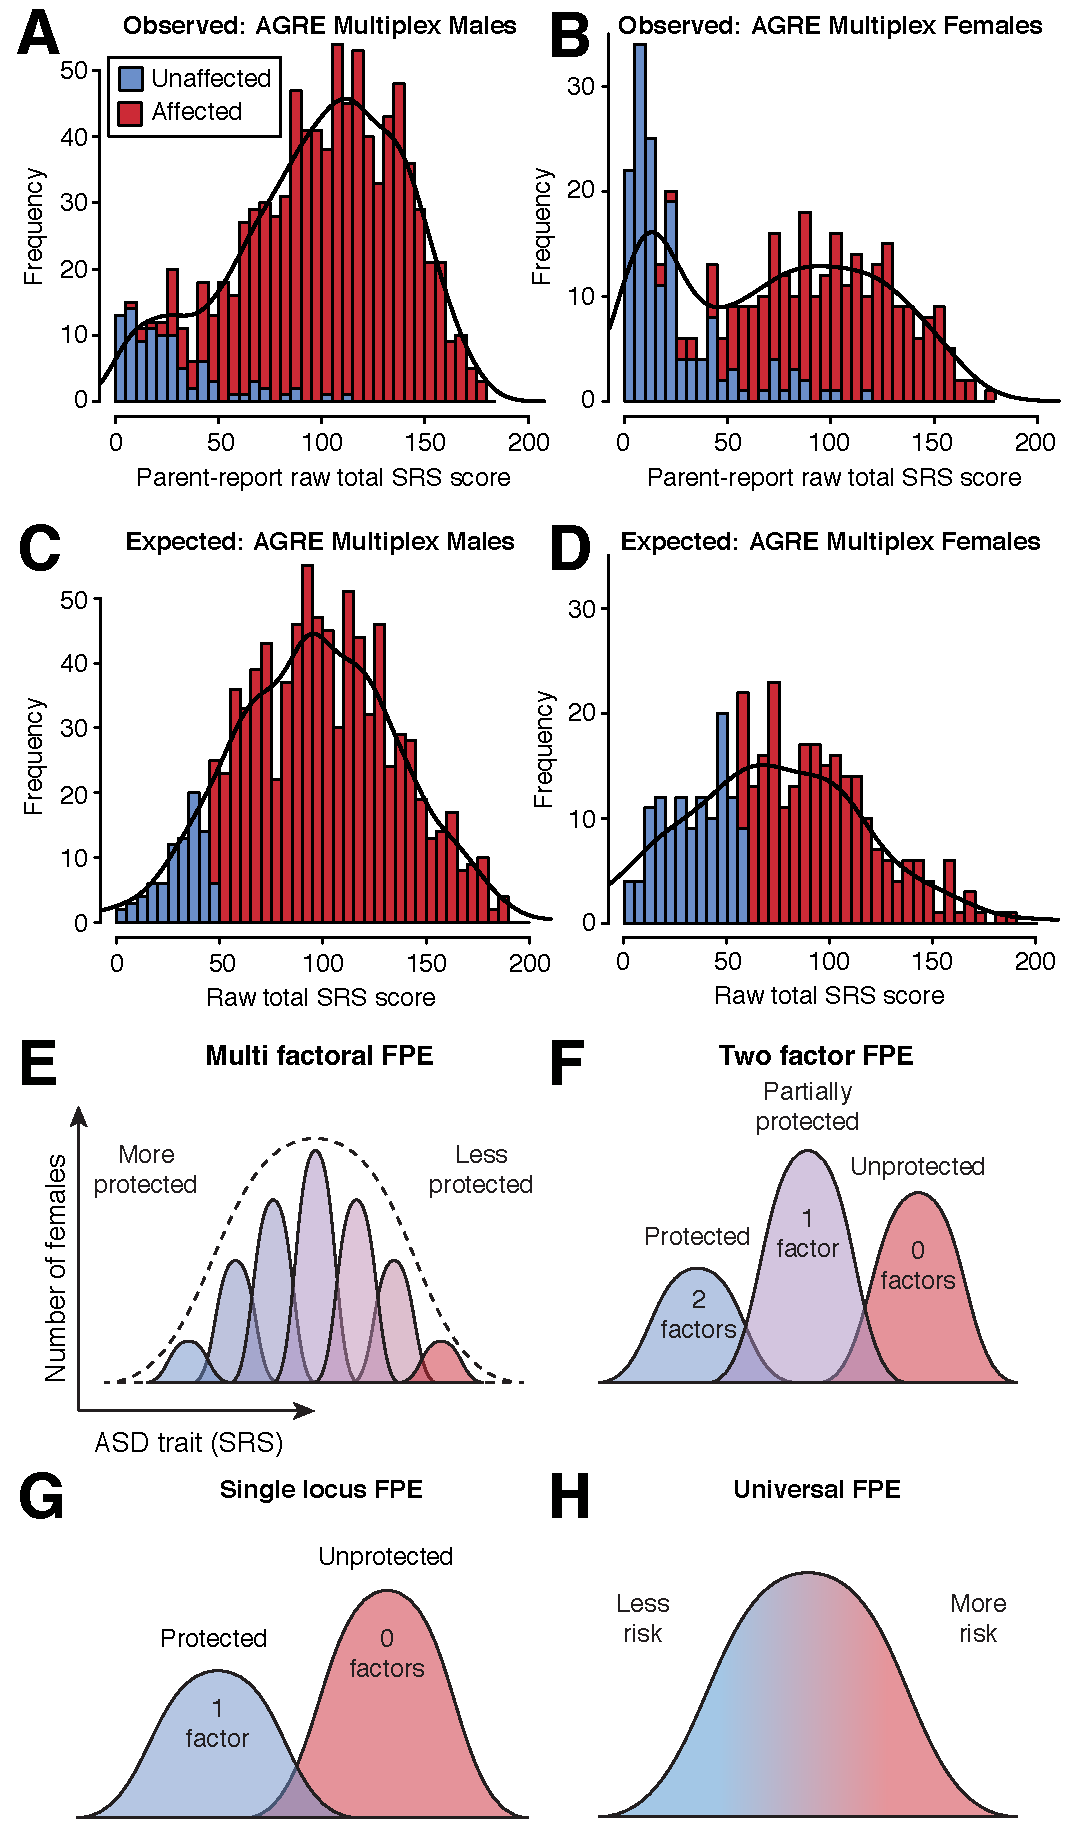
\includegraphics[width=.6\textwidth]{Figures/Figure_1_SRS_Gockley_Dec2014.pdf}
        \caption{\textbf{Expected and Observed Social Responsiveness Scale (SRS) Scores in Multiplex AGRE Families.}
        \label{Figure1}}     	
       		\scriptsize\begin{flushleft}Children in multiplex families are assumed to have inherited a high degree of ASD risk. Under a threshold model, a quantitative measure of ASD severity, such as the SRS, would be expected to follow a normal distribution with unaffected individuals at the lower end. \textbf{A)} The observed SRS scores for 927 male children (95 unaffected in blue, 832 affected in red) with each bar showing the sum of the number of unaffected and affected males. The black line shows the kernel density of the data, which approximates a normal distribution. \textbf{B)} The corresponding plot is shown for 394 female children (151 unaffected, 243 affected). The SRS scores produce a bimodal distribution, as noted previously \cite{Constantino:2010aa,Virkud:2009aa}. \textbf{C)} To assess the expected distribution under quantitative trait model the mean and standard deviation of the male observed data was estimated (A) and used these characteristics to simulate a normal distribution for the same number of individuals. The scores were sorted and a threshold for affected status was chosen to give the same number of affected and unaffected males as in ‘A’. Each bar shows the sum of the number of unaffected and affected simulated males, while the black line shows the kernel density. \textbf{D)} The expected distribution under quantitative trait model is shown using the same method as in ‘C’ but for 394 females based on the female data in ‘B’. The expected distribution differs markedly from the observed in females, but not in males. \textbf{E)} If multiple factors contribute to the presence of the FPE then their combined effect is likely to produce a unimodal distribution. \textbf{F)} As the number of factors contributing to the presence of the FPE decreases, the unimodal distribution in ‘E’ develops distinct distributions based on the number of factors present. \textbf{G)} If only one factor contributes, then a bimodal distribution should be observed. \textbf{H)} Finally, if there are no factors and the FPE is universally present in females a unimodal distribution will arise based on the distribution of risk rather than protection. 
       		\end{flushleft}
	\end{center}
    \end{figure}
	\clearpage
}\normalsize
    
    \afterpage{
        \begin{figure}[p]
			\begin{center}
			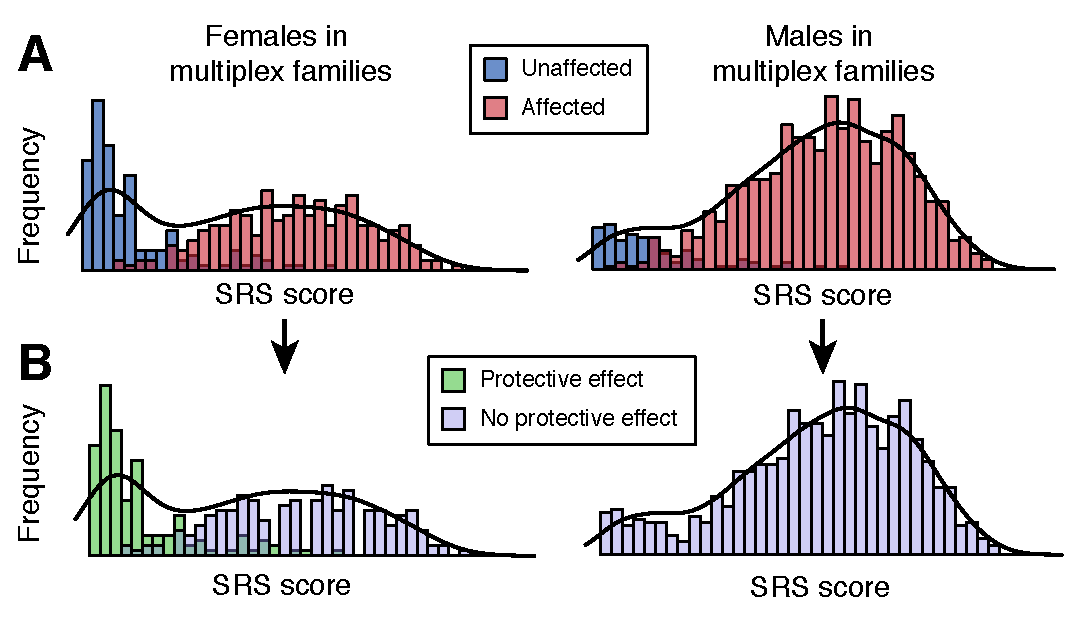
\includegraphics[width=1\linewidth]{Figures/Sup_Hypothesis_v3.pdf}
			\caption{\textbf{A Single Locus Hypothesis for the Female Protective Effect.}}
            \label{Figure2}
       		\begin{flushleft}\textbf{A)} A bimodal distribution of ASD risk, measured with the SRS, is observed for females from multiplex families but is less distinct in males. \textbf{B)} This bimodal distribution may reflect females with a protective effect (in green) vs. females without such a protective effect (in purple). 
       		\end{flushleft}
		\end{center}
    	\end{figure}
    \clearpage
	}\normalsize
	
\afterpage{
	\begin{figure}[p]
		\begin{center} 
			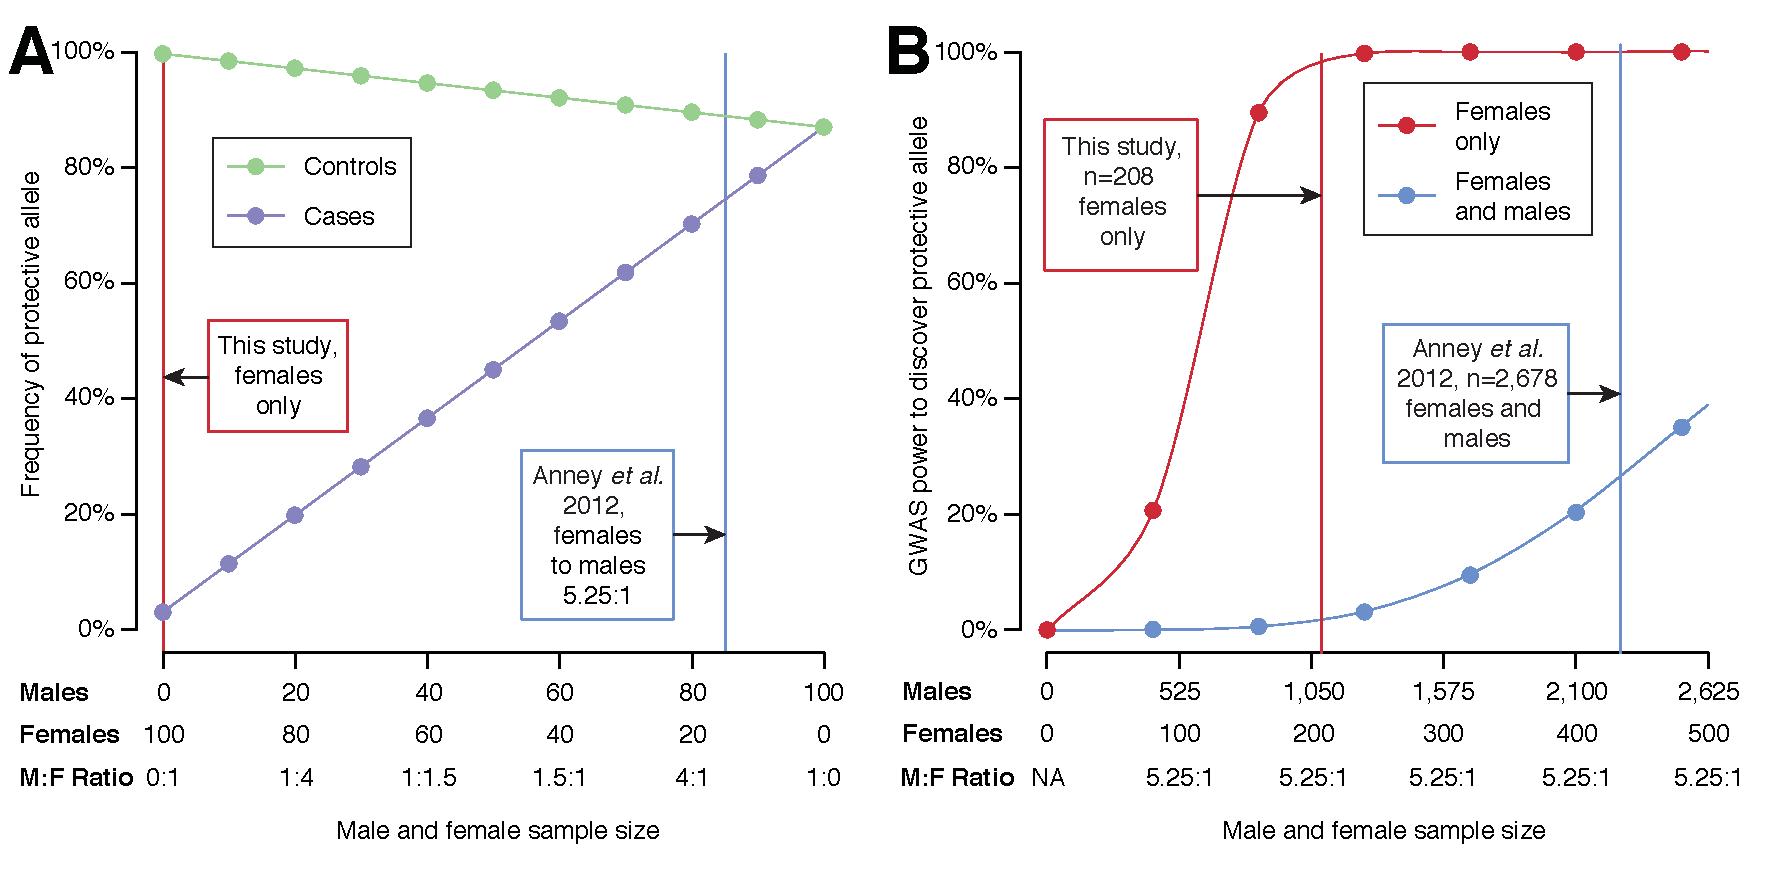
\includegraphics[width=1\linewidth]{Figures/Figure_2_Power_Gockley_Dec2014.pdf}
		\caption{\textbf{GWAS Power Estimate for a Single Factor Mediating the FPE. }\label{Figure3}}
		
       		\begin{flushleft}\textbf{A)} In females exposed to high ASD risk the protective factor will be enriched in unaffected individuals (green) and largely absent in cases (purple). A distinct difference in the frequency of the protective allele in these two cohorts can be estimated for an analysis based only on females (red line). Conversely, the protective allele has no effect in males and will be observed at an equal frequency in male cases and controls. Including males in a GWAS analysis will therefore add noise (blue line, representing the observed 5.25:1 ratio of males to females in Anney et al. 2012) resulting in a reduction in power. \textbf{B)} An estimate of GWAS power to detect a single FPE allele in females only (red) and females and males (blue) under a model where protection contributes 50\% of the observed 5.25:1 sex bias. The vertical lines represent the sample size in this study (red) and the \cite{Anney:2012aa} GWAS study (blue).
       		\end{flushleft}
	\end{center}
    \end{figure}
    \clearpage
}\normalsize

\afterpage{
        \begin{figure}[p]
			\begin{center}
			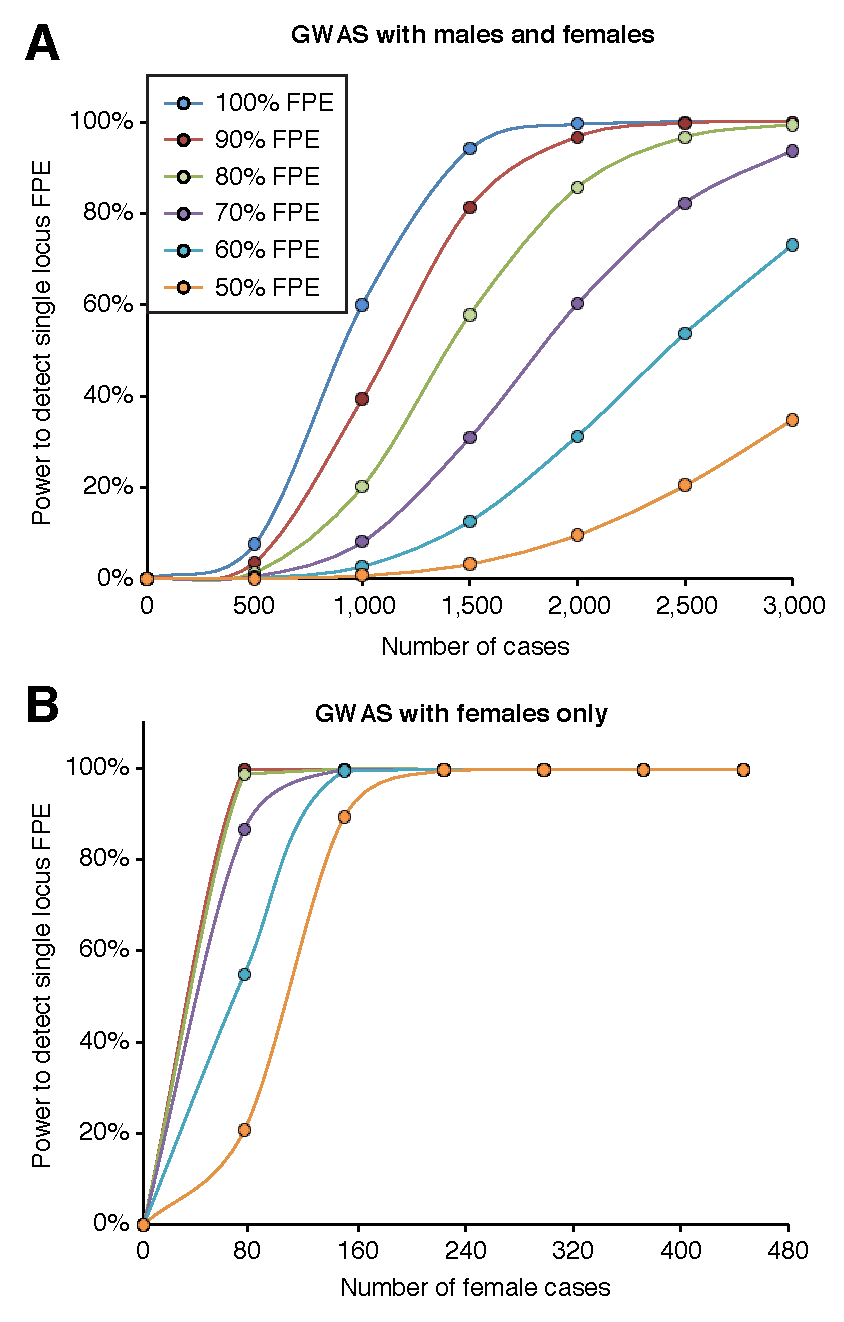
\includegraphics[width=.79\linewidth]{Figures/Power_Supp.pdf}
			\caption{\textbf{Power to Detect a Single Locus FPE.}\label{Figure4}}
			
       		\begin{flushleft}\textbf{A)} Power was estimated based of the predicated allele frequencies (Table \ref{Table1}) in affected females vs. population females. To model deviation from ideal conditions, the contribution of the FPE to ASD sex bias was decreased from 100\% to 50\%. For a given number of cases, and an equivalent number of controls, the estimated power is shown. For comparison, the largest GWAS in ASD used 2,678 cases and pseudo-controls \cite{Anney:2012aa}. \textbf{B)} The analysis is repeated for females only, based on the observed rate of 16\% \cite{Anney:2012aa}. The power is consistently greater in this female only analysis than in a conventional GWAS.
       		\end{flushleft}
	\end{center}
    \end{figure}
    \clearpage
}\normalsize
    
\afterpage{    
  	\begin{table}[p]
		\renewcommand{\arraystretch}{1}
		\begin{center}
			\begin{tabular}{|l|c|c|c|c|c|}

			\hline 
			\textbf{Category} & \textbf{PP} & \textbf{Pp} & \textbf{pP} & \textbf{pp} \\ \hline 
			Frequency in females & 75.69\% & 11.31\% & 11.31\% & 1.69\% \\ \hline 
			Frequency in affected females & 3.02\% & 45.12\% & 45.12\% & 6.74\% \\ \hline 
			Frequency in unaffected females & 99.68\% & 0.15\% & 0.15\% & 0.02\% \\ \hline 
			\end{tabular}
			
		\caption{\textbf{Predicted Frequency of p Risk Allele Under a Dominant Model in Cases and Controls}\label{Table1}}

The ``Frequency in females'' of each genotype is estimated from a \textit{P} allele frequency of 87\% and a \textit{p} allele frequency of 13\%. Under a model where the FPE reduces the incidence of ASD by 100-fold, the \textit{PP} genotype is markedly reduced in affected females. Conversely, if all females have been exposed to risk, as expected in a multiplex family, the unaffected females should be depleted for non-protective genotypes. For power calculations (Figure \ref{Figure4}) the more conservative estimate of ``Frequency in females'' was used to estimate allele frequency in unaffected females, rather than the ``Frequency in unaffected females''.
	\end{center}
    \end{table}  
	\clearpage
}\normalsize
        
\afterpage{
      \begin{figure}[p]
			\begin{center} 
			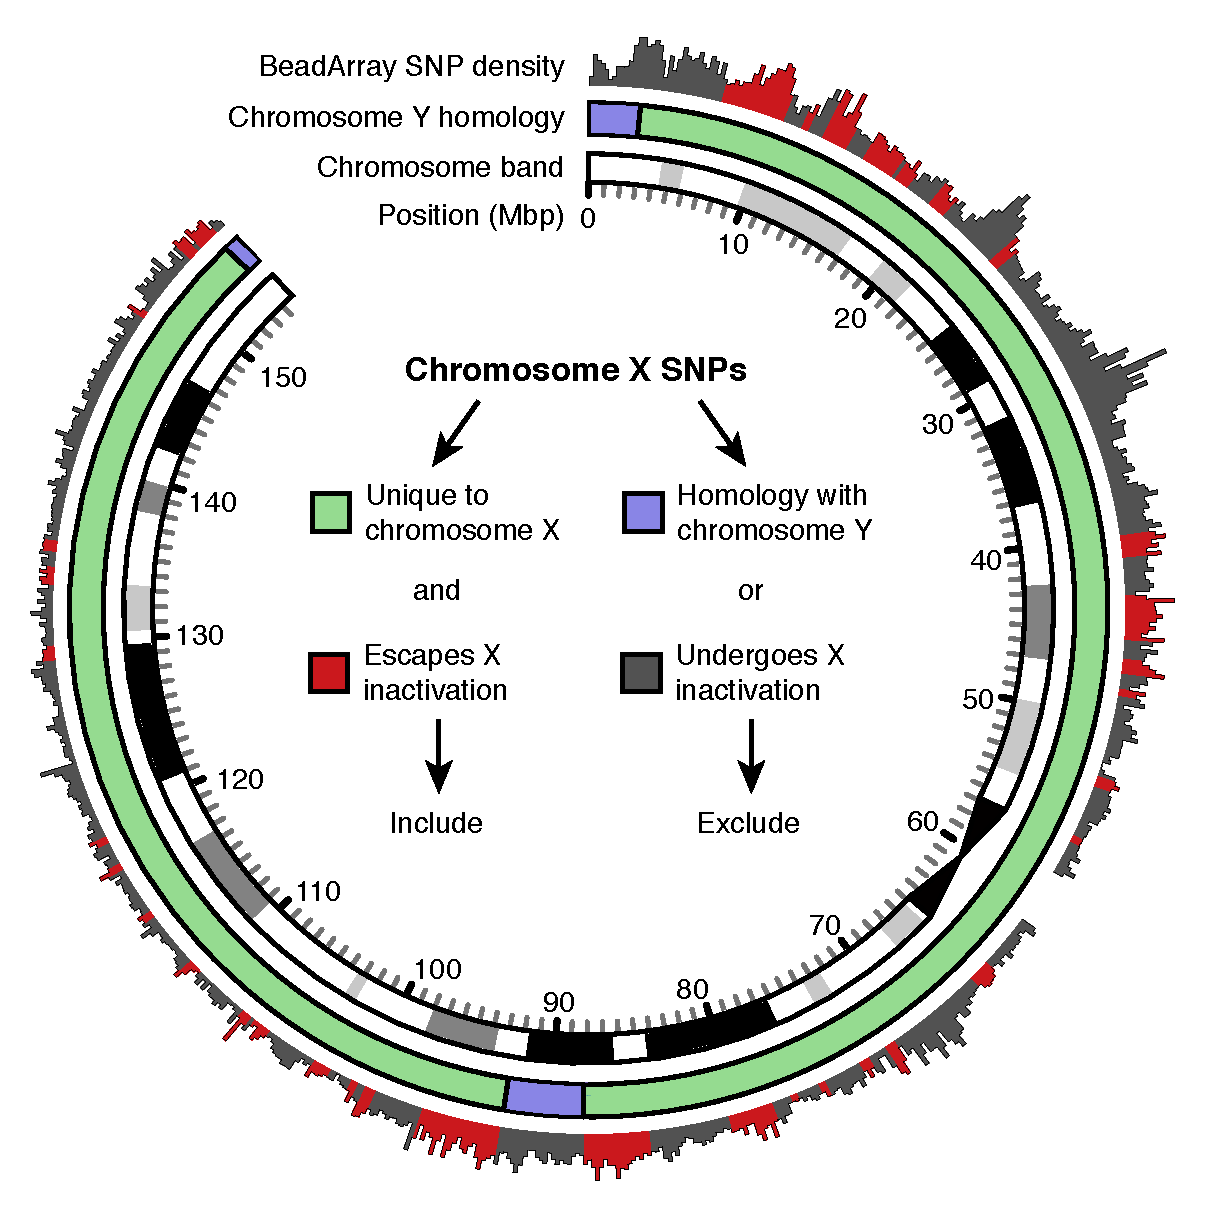
\includegraphics[width=.9\linewidth]{Figures/Figure_3_Circos_Gockley_Dec2014.pdf}
			\caption{\textbf{Identification of Chromosome X SNPs that Escape X-Inactivation for Tier 1 Analysis.}\label{Figure5}}
			
       		\begin{flushleft}This Circos plot shows the length of chromosome X proceeding clockwise with position 0 on the short arm at twelve o’clock. Adjacent to the chromosome position, the innermost ring indicates chromosome banding by the depth of shading; two opposing black arrows indicate the centromere. Regions of chromosome Y homology are shown in purple in the middle ring; SNPs in these regions were excluded from the tier 1 analysis leaving the SNPs unique to chromosome X indicated in green. The outermost ring shows SNP density based on the genotyping array (See Methods) by the height of the bars. Regions that are inactivated on one copy of chromosome X are shown in grey \cite{Carrel:2005aa} and SNPs in these regions were excluded from the tier 1 analysis, leaving only SNPs that escape X-inactivation, shown in red (Table \ref{Table1A}). Of the 6,955 SNPs on chromosome X, 451 (6.5\%) were included in the tier 1 analysis.
       		\end{flushleft}
            \end{center}
	\end{figure}
    \clearpage
}\normalsize    
   	
    \section{Methods}
    	
        \subsection{Subjects and Genotyping}
		Genotyping data were collated from two independent large cohorts of ASD families: 1,976 families from the Autism Genome Resource Exchange (AGRE) \cite{Geschwind:2001aa} and 2,733 families from the Simons Simplex Collection (SSC) \cite{Fischbach:2010aa}. The AGRE data were generated on one of three Illumina Bead Arrays: 550v1 (421 families), 550v3 (1,277 families), and Omni 1M (278 families). Analysis was restricted to the 329,483 SNPs shared between all three arrays. The SSC data were generated on one of three Illumina Bead Arrays: 1Mv1 (421 families), 1Mv3 Duo (1,277 Families), and Omni 2.5M (1,035 Families). Analysis was restricted to the 493,924 SNPs shared between all three arrays.

	\subsection{Ancestry and data cleaning}
    	Ancestry was examined as described in \cite{Anderson:2010aa}. Briefly, founders from the HapMap CEU, CHB, JPT, and YRI ancestral populations were used to train the model \cite{Duan:2008aa}. Common SNPs between all four populations and the AGRE or SSC cohort were identified in plink. Alleles were forced to the same strand, A$\to$T and G$\to$C SNPs were excluded because of alignment concerns. The final dataset was analyzed utilizing EIGENSTRAT \cite{Price:2006aa}. Samples of European ancestry in the AGRE and SSC cohort were determined by deviation in PCA components 1 and 2 between the AGRE or SSC samples and the HapMap CEU individuals. In order to be classified as European, a cohort individual was required to have a PCA component 1 and PCA component 2 value within 1.5 standard deviations of the HapMap CEU PCA component 1 and 2 means (Figure \ref{Figure6}). 
       
       Data were restricted to families of European ancestry and standard GWAS data cleaning were performed. European ancestry was determined using Eigenstrat \cite{Li:2008aa} and the four core HapMap populations Figure \ref{Figure6} [30]. The resulting genomic inflation for European samples was 1.03 Figure \ref{Figure6}. SNP data were cleaned using PLINK \cite{Purcell:2007aa}, specifically: minor allele frequency ≥0.03 (Supplementary Methods); genotype rate of ≥0.95 per sample (minimum observed genotyping rate was 0.991); genotype missingness per SNP $\leq$ 0.1; Hardy-Weinberg Equilibrium $<$ 0.0001. After data cleaning there were 943 families and 317,574 SNPs for AGRE and 2,166 families and 440,778 SNPs for SSC.\par

\subsection{Identifying Unrelated Females Through Identity by Descent}
        Of the 943 remaining AGRE families, only 510 contained at least one female with genotyping data. Where a family had multiple females only one was selected, with a preference for unaffected females, since these are less frequent in the AGRE sample. From these, 151 unaffected females and 208 affected females (defined as “Autism” or “Broad Spectrum”) were identified and used for the analysis. Identity by descent demonstrated that these samples were all unrelated, Figure \ref{Figure7}.
\par A similar approach was applied to the 2,166 remaining SSC families, of which 883 had at least one female. In families with multiple females only one was selected, with a preference for affected females, since these are less frequent in the SSC sample. The analysis was therefore performed on 207 affected females and 676 unaffected females.

	\subsection{Defining Regions Which Escape X-inactivation \& SNPs of interest}
    	For the first tier of analysis, SNPs on chromosome X were selected if they lacked homology to chromosome Y and escaped X-inactivation (Figure \ref{Figure5}, \ref{Table1A})\cite{Carrel:2005aa}. These regions represent 14\% of chromosome X (21.8Mbp). This left 451 SNPs for analysis in the AGRE data and 720 SNPs in the SSC data. For the second tier analysis all of chromosome X was considered with 6,955 SNPs in AGRE and 10,269 SNPs in SSC. Finally, for the third tier of analysis all SNPs that remained after cleaning were included with 317,574 SNPs in AGRE and 440,778 SNPs in SSC.
        Regions that escape X inactivation were determined according to the results of a gene-based rodent/human somatic cell hybrid study \cite{Carrel:2005aa}. Nine hybridomas were assessed. If gene expression was observed from an inactivated human X chromosome in at least three hybridomas, that gene was considered to escape X-inactivation. To identify regions, rather than genes, regions between consecutive escaping genes were also defined as escaping X inactivation. The co-ordinates used were defined by the first gene start position and last gene stop position plus 1kbp at either end to include regulatory regions in close proximity. UCSC gene definitions and hg18 genomic co-ordinates were used throughout (Figure \ref{Figure5}, Table \ref{Table1A}).
        
    \subsection{Hypothesized Allele Testing}
    	All analyses presented in this section are based on the hypothesis that a single common allele is responsible for a female protective effect (FPE) that produces a 4:1 sex bias in autism. There are three variables that constrain the allele frequency for such an allele: 1) The incidence of autism in the population, this assumes an estimate of 1\% \cite{Fombonne:2009aa}; 2) The observed sex bias, will use an estimate of 4:1 male to female \cite{Fombonne:2009aa}; and 3) the effect of the FPE on the incidence of ASD. The hypothesis states that the FPE is unevenly distributed between females, being present in some, but absent in others, however there is no known empirical evidence regarding how effective such protection might be under this hypothesis. Therefore, for the purposes of modeling, it is assumed that the FPE was highly effective in protecting against ASD, using an arbitrary estimate of a 100-fold reduction in risk. 

	For consistency across the different tiers of the analysis, a protective major allele (\textit{P}) and a non-protective minor allele (\textit{p}) was considered with \textit{p} acting in a dominant fashion to disrupt protection. Of note, the power calculations are unchanged if the non-protective allele acted in a recessive fashion, as the predicted difference in allele frequency between cases and controls is identical. 

	Under a dominant model, \textit{PP} confers protection, while \textit{Pp}, \textit{pP}, and \textit{pp} do not. To produce a 4:1 sex bias and 1\% ASD incidence, the \textit{P} allele must occur at a population frequency of 87\% (see Table \ref{Table2}). Under this hypothesis 76\% (87\% x 87\%) of females are protected, while the remaining 24\% lack protection.
    
	Under a model where the FPE reduces ASD incidence by 100-fold, affected females would be expected to be greatly depleted for the protective \textit{PP} genotype. Table \ref{Table3} shows the estimated percentage of females with two copies of the \textit{P} allele in the affected group and in the unaffected group, assuming all unaffected females were exposed to risk. Since only females are considered in all three tiers of the association analysis, these estimated frequencies will not change regardless of whether chromosome X or autosomes are considered. 
    
    Association tests were performed using PLINK\cite{Purcell:2007aa} under a dominant model. All p-values were corrected for multiple comparisons, using Bonferroni correction based on the number of SNPs analyzed in each tier. The cluster plots of all SNPs highlighted by the analysis are shown in Appendix \ref{AppendixC}.
    
    \subsection{Power Calculation}
 		Having estimated the frequency of the \textit{PP} genotype in affected females, the ability to detect these alleles in an association study was considered. The estimate of allele frequencies in unaffected females (Table \ref{Table3}) assumes that these subjects were exposed to risk, however this probably not the case for a subset of females due to \textit{de novo} mutations and rare inherited variants acting in a dominant manner. Therefore, the \textit{PP} genotype frequency in the population (Table \ref{Table3}, ``Frequency in females'') represents a worst case (no enrichment of unprotected females) while the \textit{PP} genotype frequency in unaffected females (Table \ref{Table3}, ``Frequency in unaffected females'') is a best case scenario. For the purposes of the power estimation, we used the population \textit{PP} genotype frequency as the more conservative approach.

		Power was estimated using G*Power3.1 \cite{Faul:2007aa} using the ``exact'' test family, ``Proportions: Inequality, two independent groups (Fisher's exact test)'', ``Post hoc: Compute achieved power - given $\alpha$, sample size, and effect size''. For power of a GWAS, two tailed analysis was selected, the frequency of the \textit{PP} genotype in affected females was entered as ``Proportion p1'' and the proportion of the \textit{PP} genotype in unaffected females was entered as ``Proportion p2''. The value used for ``$\alpha$ err prob'' was 1e-07. For sample size of each group, the number of cases and controls used was equal (in line with the pseudo-controls used)\cite{Anney:2012aa}. The results are shown in Figure \ref{Figure4}.

		This model assumes that: 1) The FPE is solely responsible for the 4:1 sex bias; 2) The hypothesized locus is solely responsible for the FPE; 3) ASD diagnosis is 100\% accurate in assessing cumulative ASD risk; and 4) The FPE reduces incidence by 100-fold. There is a high likelihood that the population effects differ from one or more of these assumptions; therefore how statistical power is affected by deviation from this model was assessed. To achieve this, the extent to which the FPE contributed to ASD sex bias was reduced. To consider a model where the FPE only contributed 50\% of sex bias, the difference between the frequency of the \textit{p} risk allele in affected and unaffected females (97\% - 24\% = 73\%) was halved (73\% / 2 = 36.5\%) and the new \textit{p} risk allele frequency in affected females was calculated by adding this difference to the \textit{p} risk allele frequency in unaffected females (24\% + 36.5\% = 60.5\%). The power calculation was repeated with this lower estimate of the \textit{p} risk allele in affected females. The results of reducing the FPE contribution are shown in Figure \ref{Figure4}.

		Reducing the contribution of the FPE to ASD sex bias is a method of testing the relative power of a conventional GWAS versus a sex-specific GWAS for this hypothesis. The decreasing contribution of the FPE can be considered as a proxy for adding noise or general deviation from the optimal predicted conditions. Of note, the sex-specific GWAS achieves considerably greater power for an equivalent sample size than a conventional GWAS (Figure \ref{Figure4}). 
 
	\subsection{SRS Based Subject Groupings of Females in Multiplex Autism Families}
 		
        It was considered that the possibility of females with and without protection may be best defined by considering SRS scores instead, or in combination, with ASD affected and unaffected diagnosis. The first exploratory analysis was based purely on parent SRS score and identified a high SRS `case' group and a low SRS `control' group (Figure \ref{Figure2}); sample sizes are based on females with high quality data and European ancestry who were used in the analysis (Table \ref{Appendix2FPEsamp}); \textbf{High SRS}: SRS $>$45, N=103 in AGRE; N=198 in SSC, \textbf{Low SRS} SRS: $\le$45, N=74 in AGRE; N=621 in SSC. No SNPs reached significance after correcting for multiple comparisons in this analysis (Figure \ref{Figure8}, \ref{Figure9}, \ref{Figure10}, \ref{Figure11}, \ref{Figure12}, \ref{Figure13} and Table \ref{Table4}).
 
 	Since AGRE is a multiplex collection, the majority of individuals are likely to carry a high burden of ASD genetic risk compared with the general population. To identify a subset of females likely to be enriched for the protective allele; first, females were classified as being affected or unaffected. Then females were further stratified within each diagnostic group by their SRS score to identify four cohorts (Figure \ref{Figure14}); sample sizes are based on samples with high quality data and European ancestry who were used in the analysis: \textbf{Affected, high SRS} (upper 50\% of all affected females; N=58 in AGRE), \textbf{Affected, low SRS} (lower 50\% of all affected females; N=51 in AGRE) \textbf{Unaffected, high SRS} (SRS $>$45; N=54 in AGRE) \textbf{Unaffected, low SRS} (SRS $\le$45; N=64 in AGRE). 
    
   Exploratory association analyses were performed with alternative definitions of the protected and unprotected groupings of females: Affected, high SRS (unprotected) vs Affected, low SRS (protected), Affected, high SRS (unprotected) vs Unaffected, high SRS (protected), Affected, high SRS (unprotected) vs Unaffected, low SRS (protected), Affected, low SRS (unprotected) vs Unaffected, high SRS (protected), Affected, low SRS (unprotected) vs Unaffected, low SRS (protected), Unaffected, high SRS (unprotected) vs Unaffected, low SRS (protected). 
 
	 None of these analyses produced SNPs with p-values exceeding the significance threshold after correction for multiple SNP comparisons (Table \ref{Table4}). Given the exploratory nature of this analysis data was not corrected for the multiple association tests.
     
     \subsection{Assessing the Impact of Ascertainment Bias on Liability}
     
     The multiplex families used in AGRE for the initial observation of a bimodal SRS distribution in females were selected on the basis of having two children affected with ASD. To assess the impact of this ascertainment bias on the distribution of ASD liability a simulation was developed.

	A male and female parent were assigned a random value for ASD liability based on a standard normal distribution (mean=0, SD=1). To model the female protective effect the mean liability in males was increased by 0.33 standard deviations and decreased by the same factor in females. These values produced a 4:1 sex bias. A diagnostic z-score threshold of 2.93 was set to produce an incidence of 1\%. 

	The mean liability of the two parents was estimated and this mean was used to estimate a random value for the ASD liability of two male children and two female children. As with the parents, the male mean was increased by 0.33, while the female mean was decreased by the same factor. If two children in the family exceeded the diagnostic threshold the family was included and the liability estimates returned.

	1 million families were simulated and the liability distribution of the male and female children were plotted (Figure \ref{Figure15}A and \ref{Figure15}B). The resulting distribution was made up of two overlapping distributions: 1) the tail end of the normal distribution cut-off at the diagnostic threshold representing the children that contributed to the ascertainment; and 2) a normal distribution with a mean above the population mean, but below the diagnostic threshold representing the children in ascertained families that did not contribute to ascertainment.

	With the addition of noise, as would be expected using a proxy measure such as the SRS, the female distribution is likely to appear bimodal while the male would be unimodal. However, this does not reproduce the initial observation of a bimodal SRS in multiplex females in two important respects: 

	\begin{enumerate}
	\item For the lower distribution in females the mean is at least one standard deviation above the population (\ref{Figure15}B), however for the SRS distribution in females the SRS scores were comparable to the normal population.

	\item The difference in male and female SRS distributions in the general population is 3 points, equivalent to 0.17 standard deviations. This is four-fold less than the difference in male and female mean used in the simulation shown in Figures \ref{Figure15}A and 	\ref{Figure15}B. Using the 0.17 standard deviation value results in the distributions shown in Figure \ref{Figure15}C and \ref{Figure15}D in which the distributions are similar between the sexes.
\end{enumerate}

	Therefore, while ascertainment bias may partially explain the bimodal SRS in multiplex females it is far from a complete explanation of this phenomena.
     
 %%Ancestry 
	\afterpage{
	\begin{figure}[p]
		\begin{center}
			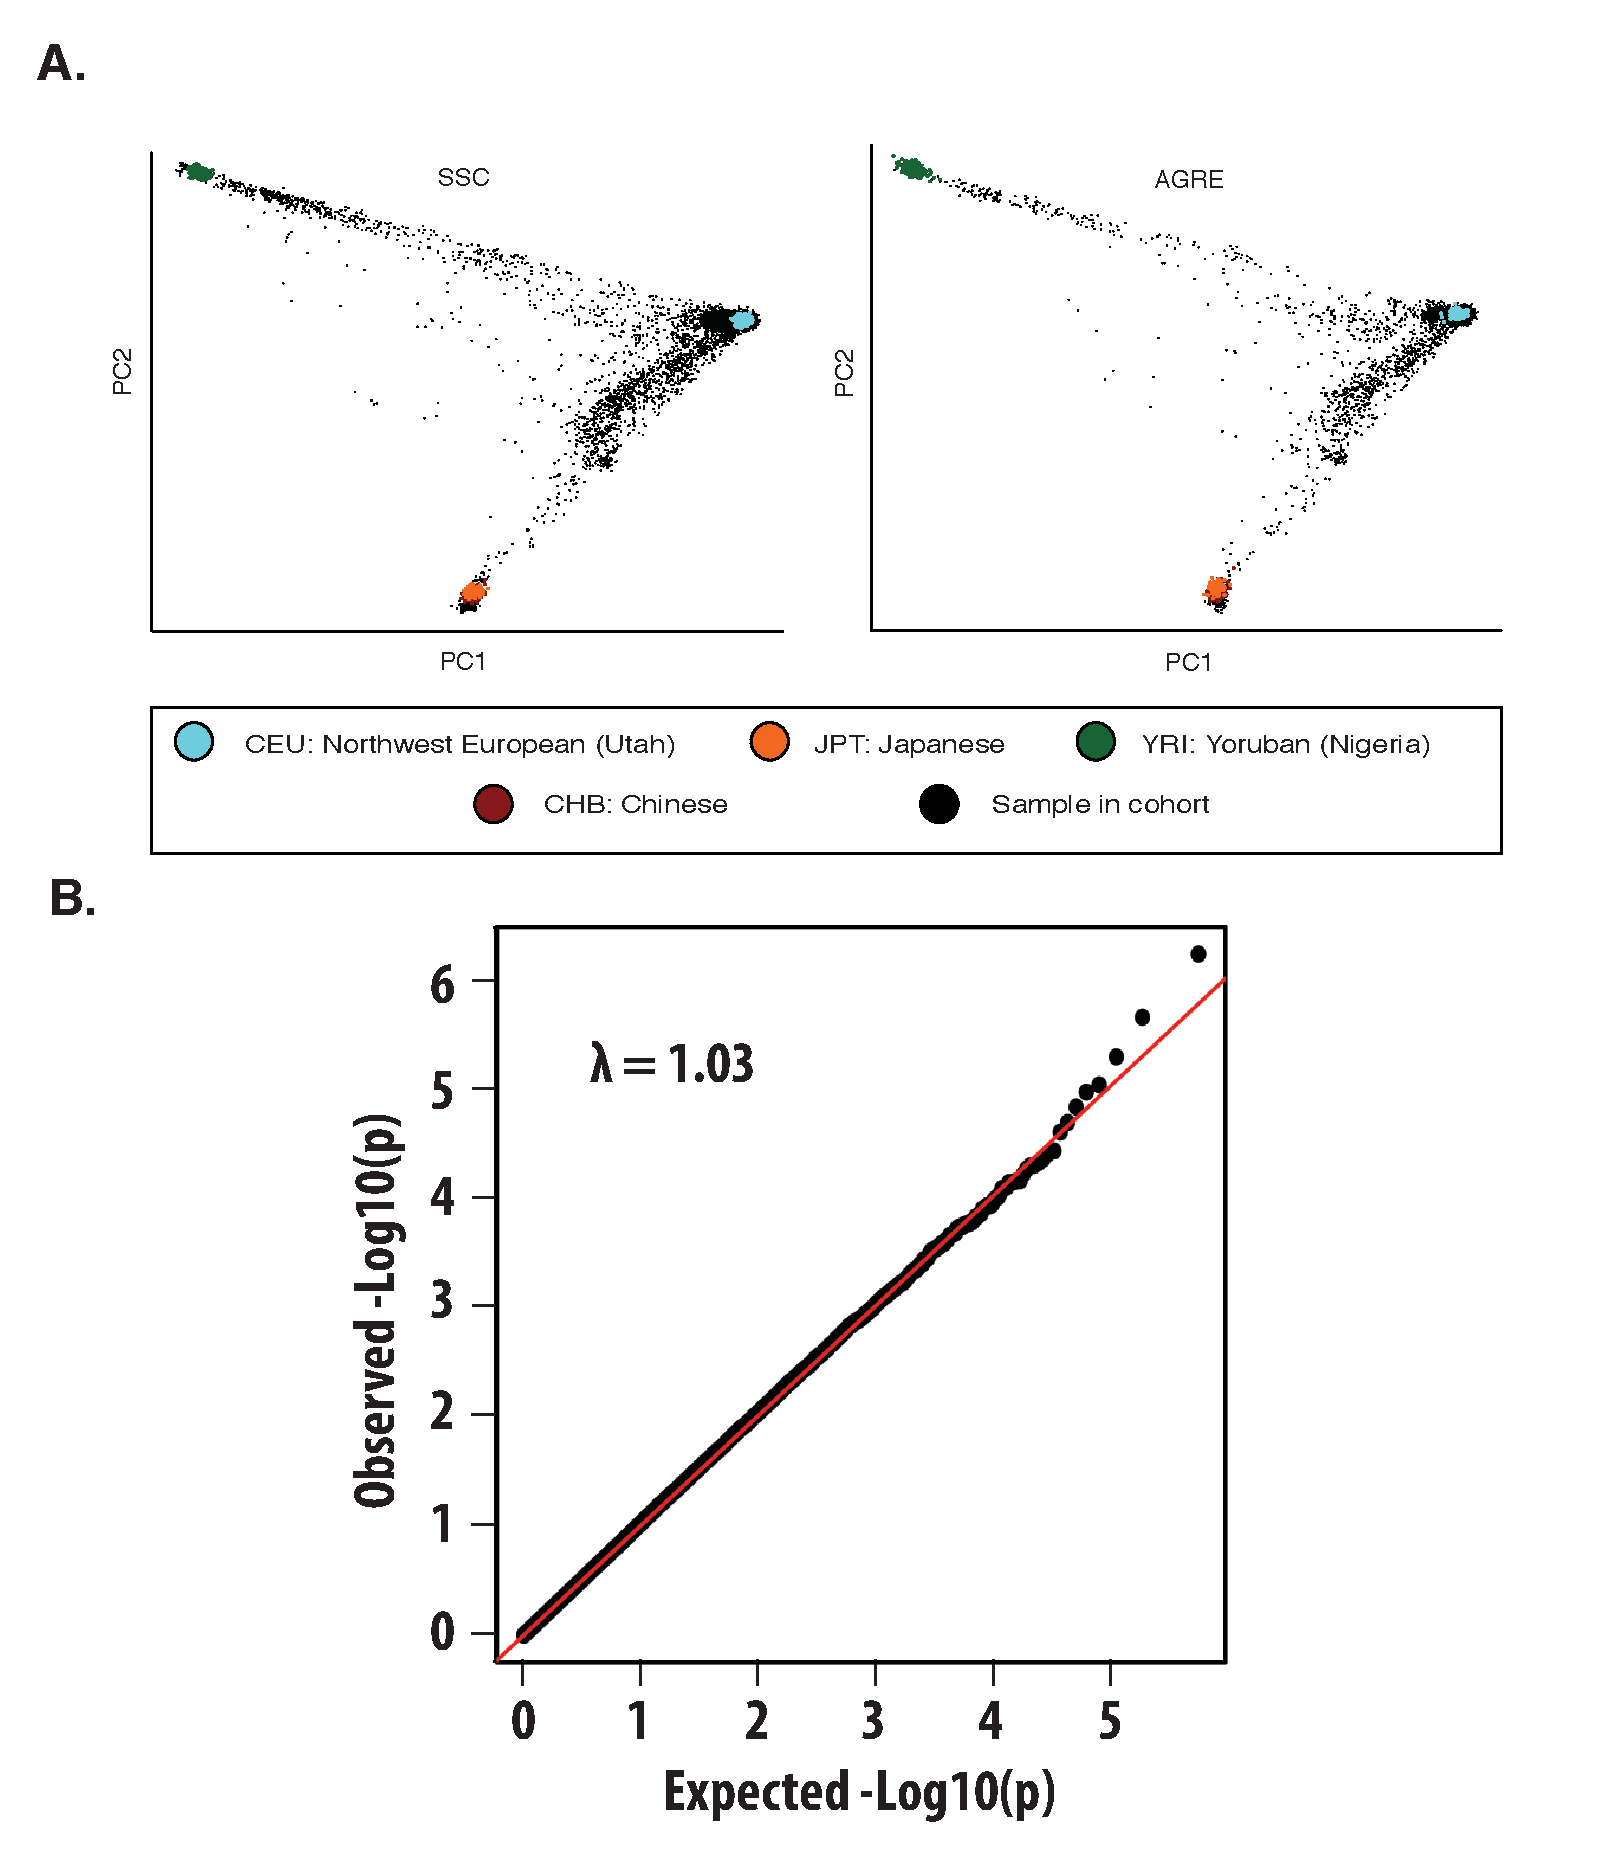
\includegraphics[width=1\linewidth, height=5.5in, keepaspectratio=TRUE]{Figures/Sup_Figure_2_v2.pdf}
		\end{center}
	\caption{\textbf{Ancestry Analysis.}\label{Figure6}}
	
	\textbf{A)} Population stratification was preformed in EIGENSTRAT. HapMap samples CEU (blue), YRI (green), JPT (Orange), and CHB (red) were used to stratify the AGRE  and SSC cohort. \textbf{B)} QQ-Plot analysis preformed on a GWAS of AGRE samples yielded a genomic inflation ($\lambda$) of 1.03.
	\end{figure}
	\clearpage
	}\normalsize
        
%%IBD
	\afterpage{
		\begin{figure}[p]
			\begin{center}
				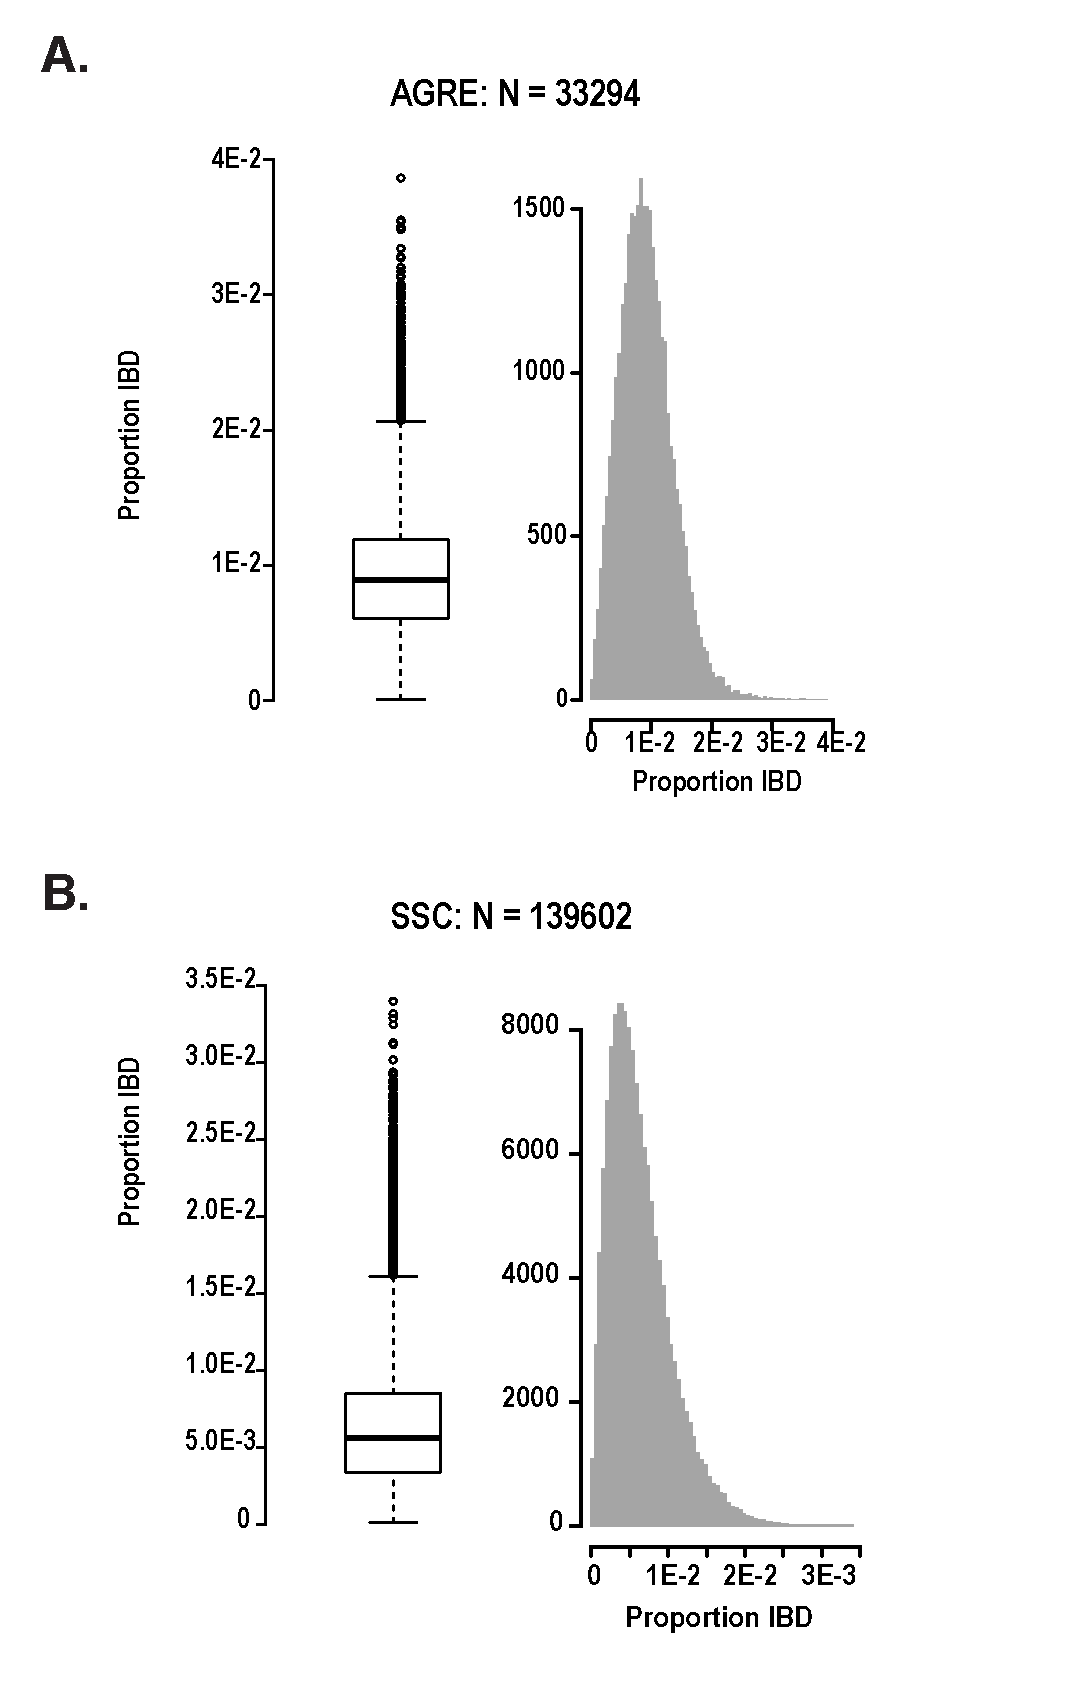
\includegraphics[width=.83\linewidth, keepaspectratio=TRUE]{Figures/Sup_Figure_3.pdf}
			\end{center}
			\caption{\textbf{Identity by Descent (IBD) Analysis.}\label{Figure7}}
			
			\textbf{A)} 33,294 (51.8\%) of the pairwise comparisons between samples in the AGRE cohort registered an IBD proportion greater than 0. All pairwise IBD comparisons yielded a value below 4\%. \textbf{B)} 139,602 (35.9\%) of the pairwise comparisons between samples in the SSC cohort registered an IBD proportion greater than 0. All pairwise IBD comparisons yielded a value below 3.5\%.
		\end{figure}       
    \clearpage
	}\normalsize
    
%%Table S2 from paper 
%%Predicted Allele Frequency - Single Locus
\afterpage{
	\begin{table}[p]
		\renewcommand{\arraystretch}{1}
		\begin{center}
			\begin{tabular}{|l|c|c|c|c|c|c|}

				\hline 
				\textbf{Category} & \textbf{PP} & \textbf{Pp} & \textbf{pP} & \textbf{pp} & \textbf{P} & \textbf{p} \\ \hline 
Sex & \multicolumn{4}{|c|}{Female} & \multicolumn{2}{|c|}{Male}  \\ \hline 
Protective effect & Present & \multicolumn{3}{|c|}{Absent} & \multicolumn{2}{|c|}{Absent} \\ \hline 
Population Frequency & 37.8\% & 5.7\% & 5.7\% & 0.8\% & 43.5\% & 6.5\% \\ \hline 
ASD incidence & 0.016\% & 1.6\% & 1.6\% & 1.6\% & 1.6\% & 1.6\% \\ \hline 
Population ASD incidence & 0.006\% & 0.09\% & 0.09\% & 0.01\% & 0.70\% & 0.10\% \\ \hline 
Population ASD incidence & \multicolumn{4}{|c|}{0.20\%} & \multicolumn{2}{|c|}{0.80\%} \\ \hline 
Sex ratio & \multicolumn{4}{|c|}{1.0} & \multicolumn{2}{|c|}{4.0}  \\ \hline 
Total population incidence & \multicolumn{6}{|c|}{1.00\%}  \\ \hline 

			\end{tabular}
			\caption{\textbf{Predicted Allele Frequency of Single Locus FPE}\label{Table2}}
			
		\end{center}
The presence of a simple bimodal distribution raises the possibility that a protective allele (\textit{P}) at a single locus could produce the female protective effect; protection mediated by two copies of the allele (\textit{PP}) would be limited to females. Furthermore, a population allele frequency of 87\% for \textit{P}, and 13\% for the non-protective \textit{p} allele, leads to the observed ASD sex ratio of 4:1. ``Population frequency'' is calculated by: 50\% (percent of population of that sex) x allele 1 frequency x allele 2 frequency. ``ASD incidence'' is estimated based on a total ASD incidence of 1.0\% and an arbitrary 100x reduction in incidence when the female protective effect is present. ``Population ASD incidence'' is estimated by ``Population frequency'' multiplied by ``ASD incidence'' and these are summed to give ``ASD incidence'' by sex and ``Total population incidence''. The ratio of ``ASD incidence'' by sex gives the ``Sex ratio''. A \textit{P} allele frequency of 87\% is the only value to produce a 4:1 sex ratio and 1\% ASD incidence. Decreasing the effectiveness of the FPE from 100-fold requires the allele frequency of \textit{P} to increase.
	\end{table}
	\clearpage
}\normalsize

%%Predicted Allele Frequency - Dominant Model
\afterpage{
	\begin{table}[p]
		\renewcommand{\arraystretch}{1}
		\begin{center}
		\begin{tabular}{|l|c|c|c|c|c|}
			\hline 
			\textbf{Category} & \textbf{PP} & \textbf{Pp} & \textbf{pP} & \textbf{pp} \\ \hline 
Frequency in females & 75.69\% & 11.31\% & 11.31\% & 1.69\% \\ \hline 
Frequency in affected females & 3.02\% & 45.12\% & 45.12\% & 6.74\% \\ \hline 
Frequency in unaffected females & 99.68\% & 0.15\% & 0.15\% & 0.02\% \\ \hline 
		\end{tabular}
		\caption{\textbf{Predicted Frequency of p Risk Allele Under a Dominant Model in Cases and Controls}\label{Table3}}
		
		\end{center}
The ``Frequency in females'' of each genotype is estimated from a \textit{P} allele frequency of 87\% and a \textit{p} allele frequency of 13\%. Under a model where the FPE reduces the incidence of ASD by 100-fold, the \textit{PP} genotype is markedly reduced in affected females. Conversely, if all females have been exposed to risk, as expected in a multiplex family, the unaffected females should be depleted for non-protective genotypes. For power calculations (Figures \ref{Figure3} and \ref{Figure4}) the more conservative estimate of ``Frequency in females'' was used to estimate allele frequency in unaffected females, rather than the ``Frequency in unaffected females''.
	\end{table}
    \clearpage
}\normalsize

%%Dominant Model
\afterpage{
	\begin{figure}[p]
		\begin{center}
			%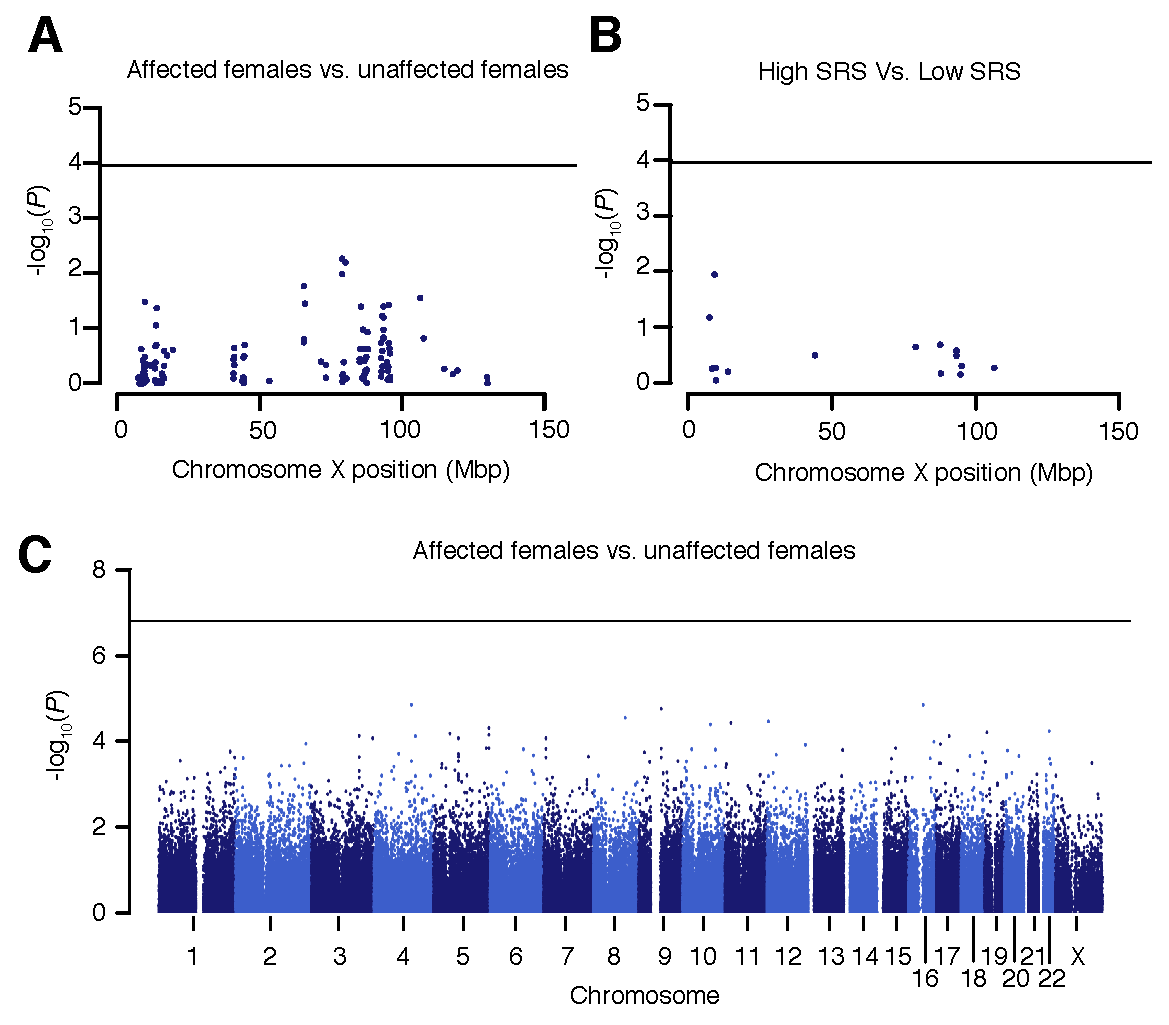
\includegraphics[width=\linewidth]{Sup_4_AGRE_Dom.pdf}
			\includegraphics[width=1\linewidth]{Figures/ONE.png}
		\end{center}
		\caption{\textbf{Manhattan Plot of Association Results Under a Dominant Model in the AGRE Cohort. }\label{Figure8}}
		
		\textbf{A)} Loci on the X-Chromosome within regions shown to escape X-inactivation were examined between cases and controls in AGRE. The association test results under a dominant model are shown. \textbf{B)} The analysis was repeated using an SRS cut off value of 45 was used to distinguish cases (high SRS) from controls (low SRS), instead of ASD diagnostic status. \textbf{C)} Using ASD diagnosis to identify cases and controls a genome-wide association analysis with a dominant model was performed. 
	\end{figure}
	\clearpage
}\normalsize

\afterpage{
	\begin{figure}[p]
		\begin{center}
			%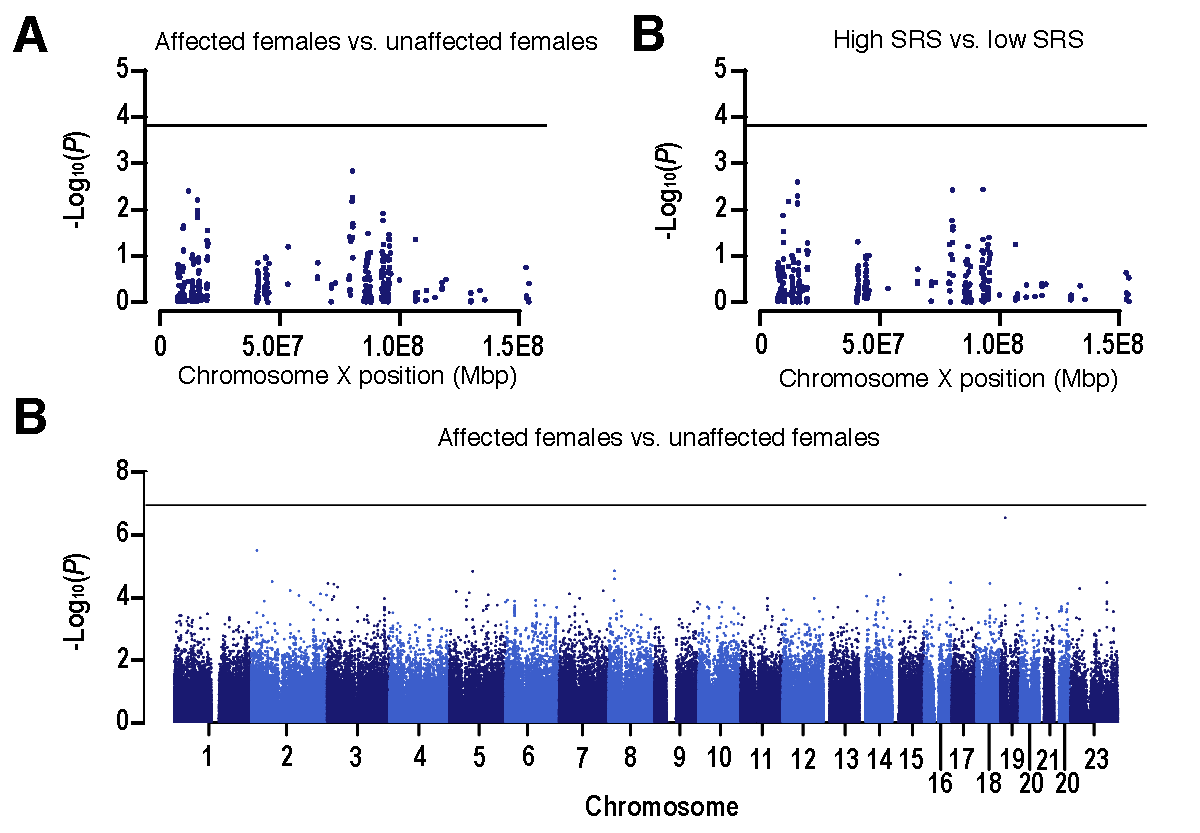
\includegraphics[width=\linewidth]{Sup_5_SSC_DomRast.pdf}
			\includegraphics[width=1\linewidth]{Figures/TWO.png}
		\end{center}

		\caption{\textbf{Manhattan Plot of Association Results Under a Dominant Model in the SSC Cohort. }\label{Figure9}}
		
		\textbf{A)} Loci on the X-Chromosome within regions shown to escape X-inactivation were examined between cases and controls in SCC. The association test results under a dominant model are shown. \textbf{B)} The analysis was repeated using an SRS cut off value of 45 was used to distinguish cases (high SRS) from controls (low SRS), instead of ASD diagnostic status. \textbf{C)} Using ASD diagnosis to identify cases and controls a genome-wide association analysis with a dominant model was performed. 
	\end{figure}
	\clearpage
}\normalsize

%%Recessive Model
\afterpage{
	\begin{figure}[p]
		\begin{center}
			%\includegraphics[width=\linewidth]{Sup_6_AGRE_Rec.pdf}
			\includegraphics[width=1\linewidth]{Figures/THREE.png}
		\end{center}
		\caption{\textbf{Manhattan Plot of Association Results Under a Recessive Model in the AGRE Cohort. }\label{Figure10}}
		
		\textbf{A)} Loci on the X-Chromosome within regions shown to escape X-inactivation were examined between cases and controls in AGRE. The association test results under a recessive model are shown. \textbf{B)} The analysis was repeated using an SRS cut off value of 45 was used to distinguish cases (high SRS) from controls (low SRS), instead of ASD diagnostic status. \textbf{C)} Using ASD diagnosis to identify cases and controls a genome-wide association analysis with a recessive model was performed. 
	\end{figure}
	\clearpage
}\normalsize

\afterpage{
	\begin{figure}[p]
	\begin{center}
			%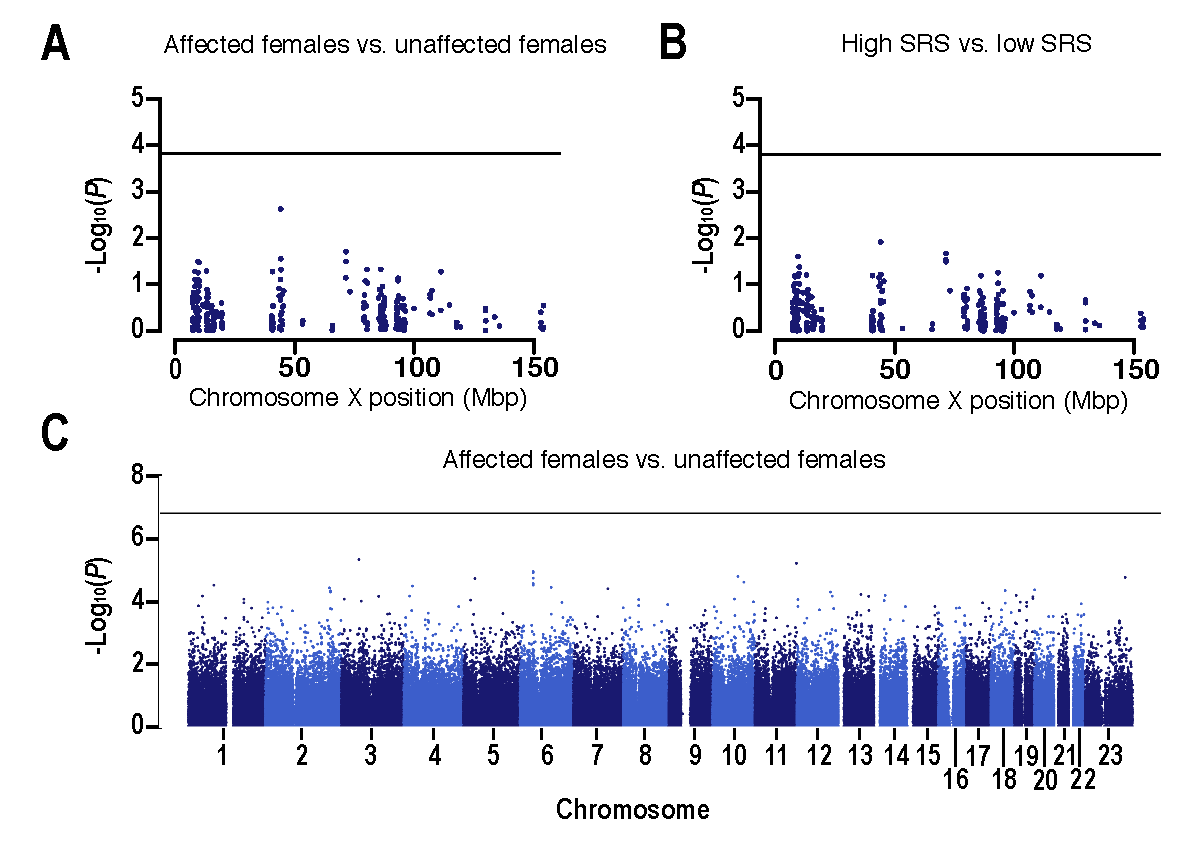
\includegraphics[width=\linewidth]{Sup_7_SSC_RecRast.pdf}
			\includegraphics[width=1\linewidth]{Figures/FOUR.png}
		\end{center}
		\caption{\textbf{Manhattan Plot of Association Results Under a Recessive Model in the SSC Cohort. }\label{Figure11}}
		
		\textbf{A)} Loci on the X-Chromosome within regions shown to escape X-inactivation were examined between cases and controls in SSC. The association test results under a recessive model are shown. \textbf{B)} The analysis was repeated using an SRS cut off value of 45 was used to distinguish cases (high SRS) from controls (low SRS), instead of ASD diagnostic status. \textbf{C)} Using ASD diagnosis to identify cases and controls a genome-wide association analysis with a recessive model was performed. 
	\end{figure}
	\clearpage
}\normalsize

%%Additive Model
\afterpage{
	\begin{figure}[p]
		\begin{center}
			%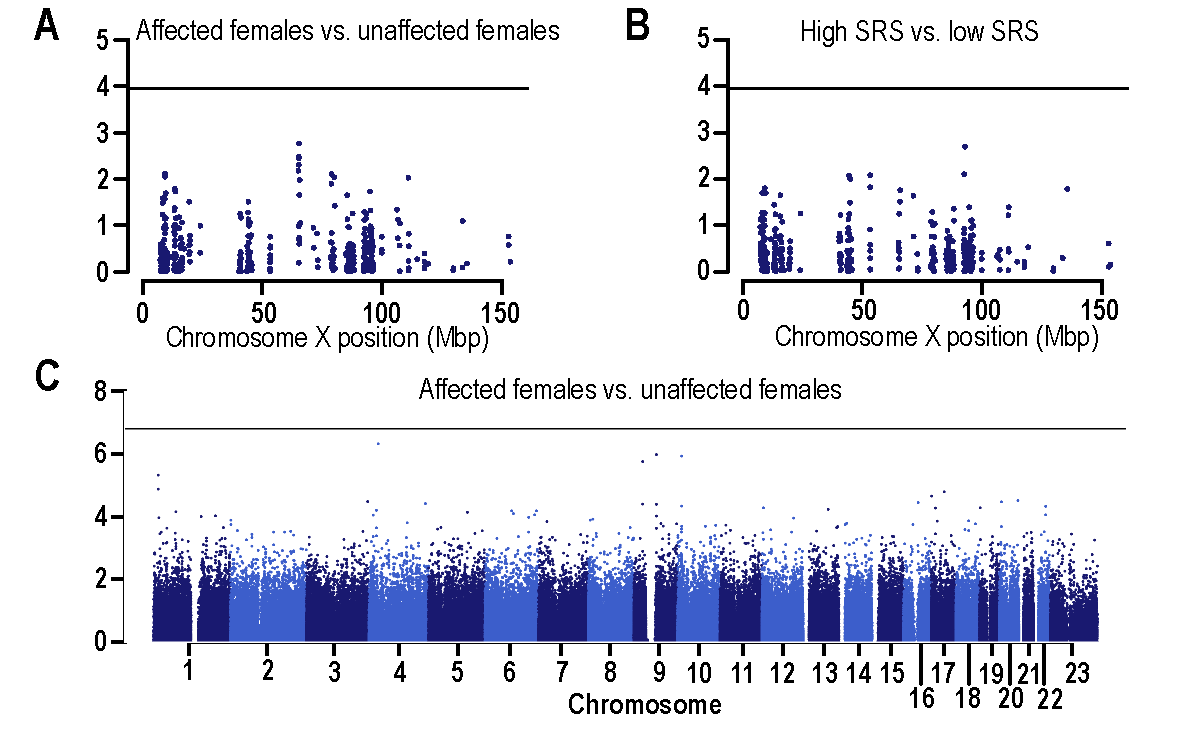
\includegraphics[width=\linewidth]{AGRE_Default_Rast.pdf}
			\includegraphics[width=1\linewidth]{Figures/FIVE.png}
		\end{center}
		\caption{\textbf{Manhattan Plot of Association Results Under an Additive Model in the AGRE Cohort. }\label{Figure12}}
		
		\textbf{A)} Loci on the X-Chromosome within regions shown to escape X-inactivation were examined between cases and controls in SSC. The association test results under a recessive model are shown. \textbf{B)} The analysis was repeated using an SRS cut off value of 45 was used to distinguish cases (high SRS) from controls (low SRS), instead of ASD diagnostic status. \textbf{C)} Using ASD diagnosis to identify cases and controls a genome-wide association analysis with a recessive model was performed. 
	\end{figure}
	\clearpage
}\normalsize

\afterpage{
	\begin{figure}[p]
		\begin{center}
			%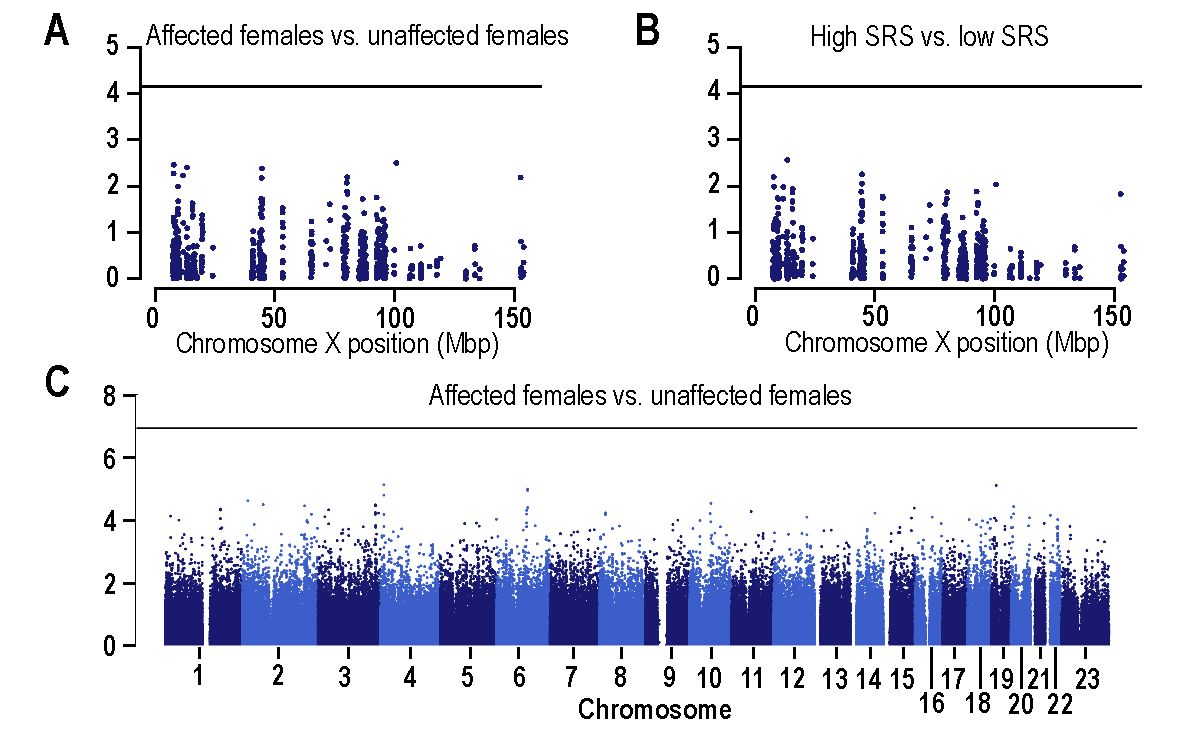
\includegraphics[width=\linewidth]{SSC_Default_Rast.pdf}
			\includegraphics[width=1\linewidth]{Figures/SIX.png}
		\end{center}
		\caption{\textbf{Manhattan Plot of Association Results Under an Additive Model in the SSC Cohort. }\label{Figure13}}
		
		\textbf{A)} Loci on the X-Chromosome within regions shown to escape X-inactivation were examined between cases and controls in SSC. The association test results under a recessive model are shown. \textbf{B)} The analysis was repeated using an SRS cut off value of 45 was used to distinguish cases (high SRS) from controls (low SRS), instead of ASD diagnostic status. \textbf{C)} Using ASD diagnosis to identify cases and controls a genome-wide association analysis with a recessive model was performed. 
	\end{figure}
	\clearpage
}\normalsize

%%Alternate Anaylsis SNP table
\afterpage{
	\renewcommand{\arraystretch}{.95}%
	\begin{table}[p]
		\begin{center}
			\begin{tabular}{cccccc}

				Comparison&SNP&Chr&Position&P-Val&BF-Corrected\\		
				\hline													
				\\            

				 &rs7891218 & X & 92838948 & 2.0E-03 & 0.91 \\ 
				High SRS & rs5983514 & X & 92560942 & 7.9E-03 & 1 \\ 
				Versus & rs1409117 & X & 53319220 & 8.4E-03 & 1 \\ 
				Low SRS & rs2146335 & X & 44389803 & 8.6E-03 & 1 \\ 
				 & rs7050908 & X & 44918083 & 1.0E-02 & 1 \\ 

				\hline													
				\\

				 & rs6524008 & X & 107483616 & 4.4E-03 & 1 \\
				Affected, high SRS & rs6622146 & X & 106209321 & 4.6E-03 & 1 \\
				Versus & rs12014086 & X & 44065595 & 6.9E-03 & 1 \\
				Affected, low SRS & rs5990206 & X & 95558656 & 9.6E-03 & 1 \\
				 & rs10521610 & X & 10124322 & 1.0E-02 & 1 \\
				\hline													
				\\	

				 & rs12012307 & X & 19803729 & 3.4E-03 & 1 \\
				Affected, high SRS & rs4350137 & X & 93943526 & 4.2E-03 & 1 \\
				Versus & rs727090 & X & 13469667 & 4.6E-03 & 1 \\
				Unaffected, high SRS & rs1017874 & X & 19779567 & 5.7E-03 & 1 \\
				 & rs2285405 & X & 119262477 & 8.7E-03 & 1 \\
				\hline													
				\\	

				 & rs881599 & X & 9135603 & 2.7E-03 & 1 \\
				Affected, high SRS & rs2317959 & X & 94641848 & 3.9E-03 & 1 \\
				Versus & rs2074098 & X & 13735538 & 5.3E-03 & 1 \\
				Unaffected, low SRS & rs5978769 & X & 7808157 & 1.5E-02 & 1 \\
				 & rs12688370 & X & 13806166 & 1.6E-02 & 1 \\
				\hline													
				\\	

				 & rs5935671 & X & 13786582 & 2.0E-03 & 0.89 \\
				Affected, low SRS & rs5990206 & X & 95558656 & 2.9E-03 & 1 \\
				Versus & rs5936079 & X & 15867223 & 3.7E-03 & 1 \\
				Unaffected, high SRS & rs234495 & X & 15348936 & 7.1E-03 & 1 \\
				 & rs11796661 & X & 86749681 & 8.7E-03 & 1 \\
				\hline													
				\\	

				 & rs6622146 & X & 106209321 & 3.1E-03 & 1 \\
				Affected, low SRS & rs5949895 & X & 95725873 & 5.6E-03 & 1 \\
				Versus & rs1983481 & X & 8292613 & 7.0E-03 & 1 \\
				Unaffected, low SRS & rs5990153 & X	& 95028102 & 1.3E-02 & 1 \\
				 & rs12688370 & X & 13806166 & 1.3E-02 & 1 \\
				\hline													
				\\	

				& rs5949895 & X & 95725873 & 5.6E-04 & 0.25 \\
				Unaffected, high SRS & rs234495 & X & 15348936 & 2.9E-03 & 1 \\
				Versus & rs5936079 & X & 15867223 & 1.0E-02 & 1 \\
				Unaffected, low SRS & rs5913240 & X & 79384683 & 1.0E-02 & 1 \\
				& rs12834592 & X & 92669150 & 1.2E-02 & 1 \\
				\hline													
				\\	
				\end{tabular}
			\caption{\textbf{AGRE Association Test Results Based on SRS Defined Case/Control Definitions }\label{Table4}}
			
		\end{center}
		Considering the possibility that the protective status of the females may not correlate well with ASD diagnosis, we compared females in AGRE based on a combination of SRS and ASD categorical diagnosis (Figure \ref{Figure14}). The top five SNPs in each analysis are shown.
	\end{table}
	\clearpage
}\normalsize

%%AGRE Stratification
\afterpage{
	\begin{figure}[p]
		\begin{center}
			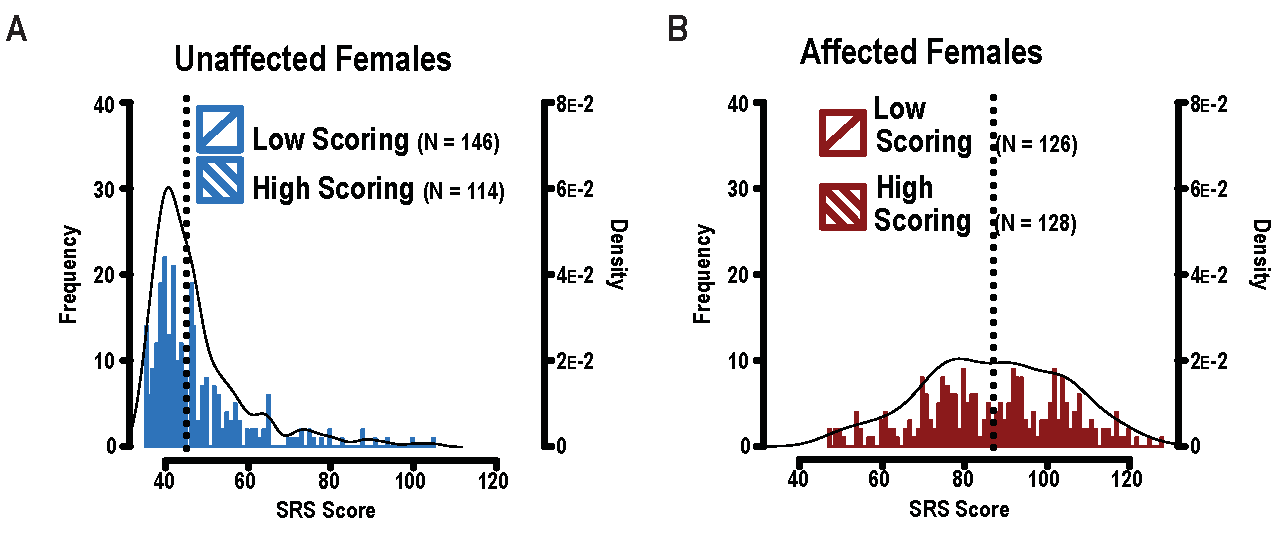
\includegraphics[width=1\linewidth, height=6.5in, keepaspectratio=TRUE]{Figures/Sup_8.pdf}
		\end{center}
		\caption{\textbf{Stratification of AGRE Affected and Unaffected Females by SRS Score.}\label{Figure14}}
		
		\textbf{A)} Unaffected females were stratified into a higher scoring (N=114) and lower scoring (N=146) population based on an SRS score of 45. After data cleaning, and considering only unrelated samples of European ancestry, the samples sizes were 54 and 64 respectively. \textbf{B)} Affected females were stratified at the 50th percentile into higher scoring (N=128) and lower scoring (N=126) groups. After data cleaning, and considering only unrelated samples of European ancestry, the samples sizes were 58 and 51 respectively.
	\end{figure}
	\clearpage
}\normalsize


%%Ascertainment Bias
\afterpage{
	\begin{figure}[p]
		\begin{center}
			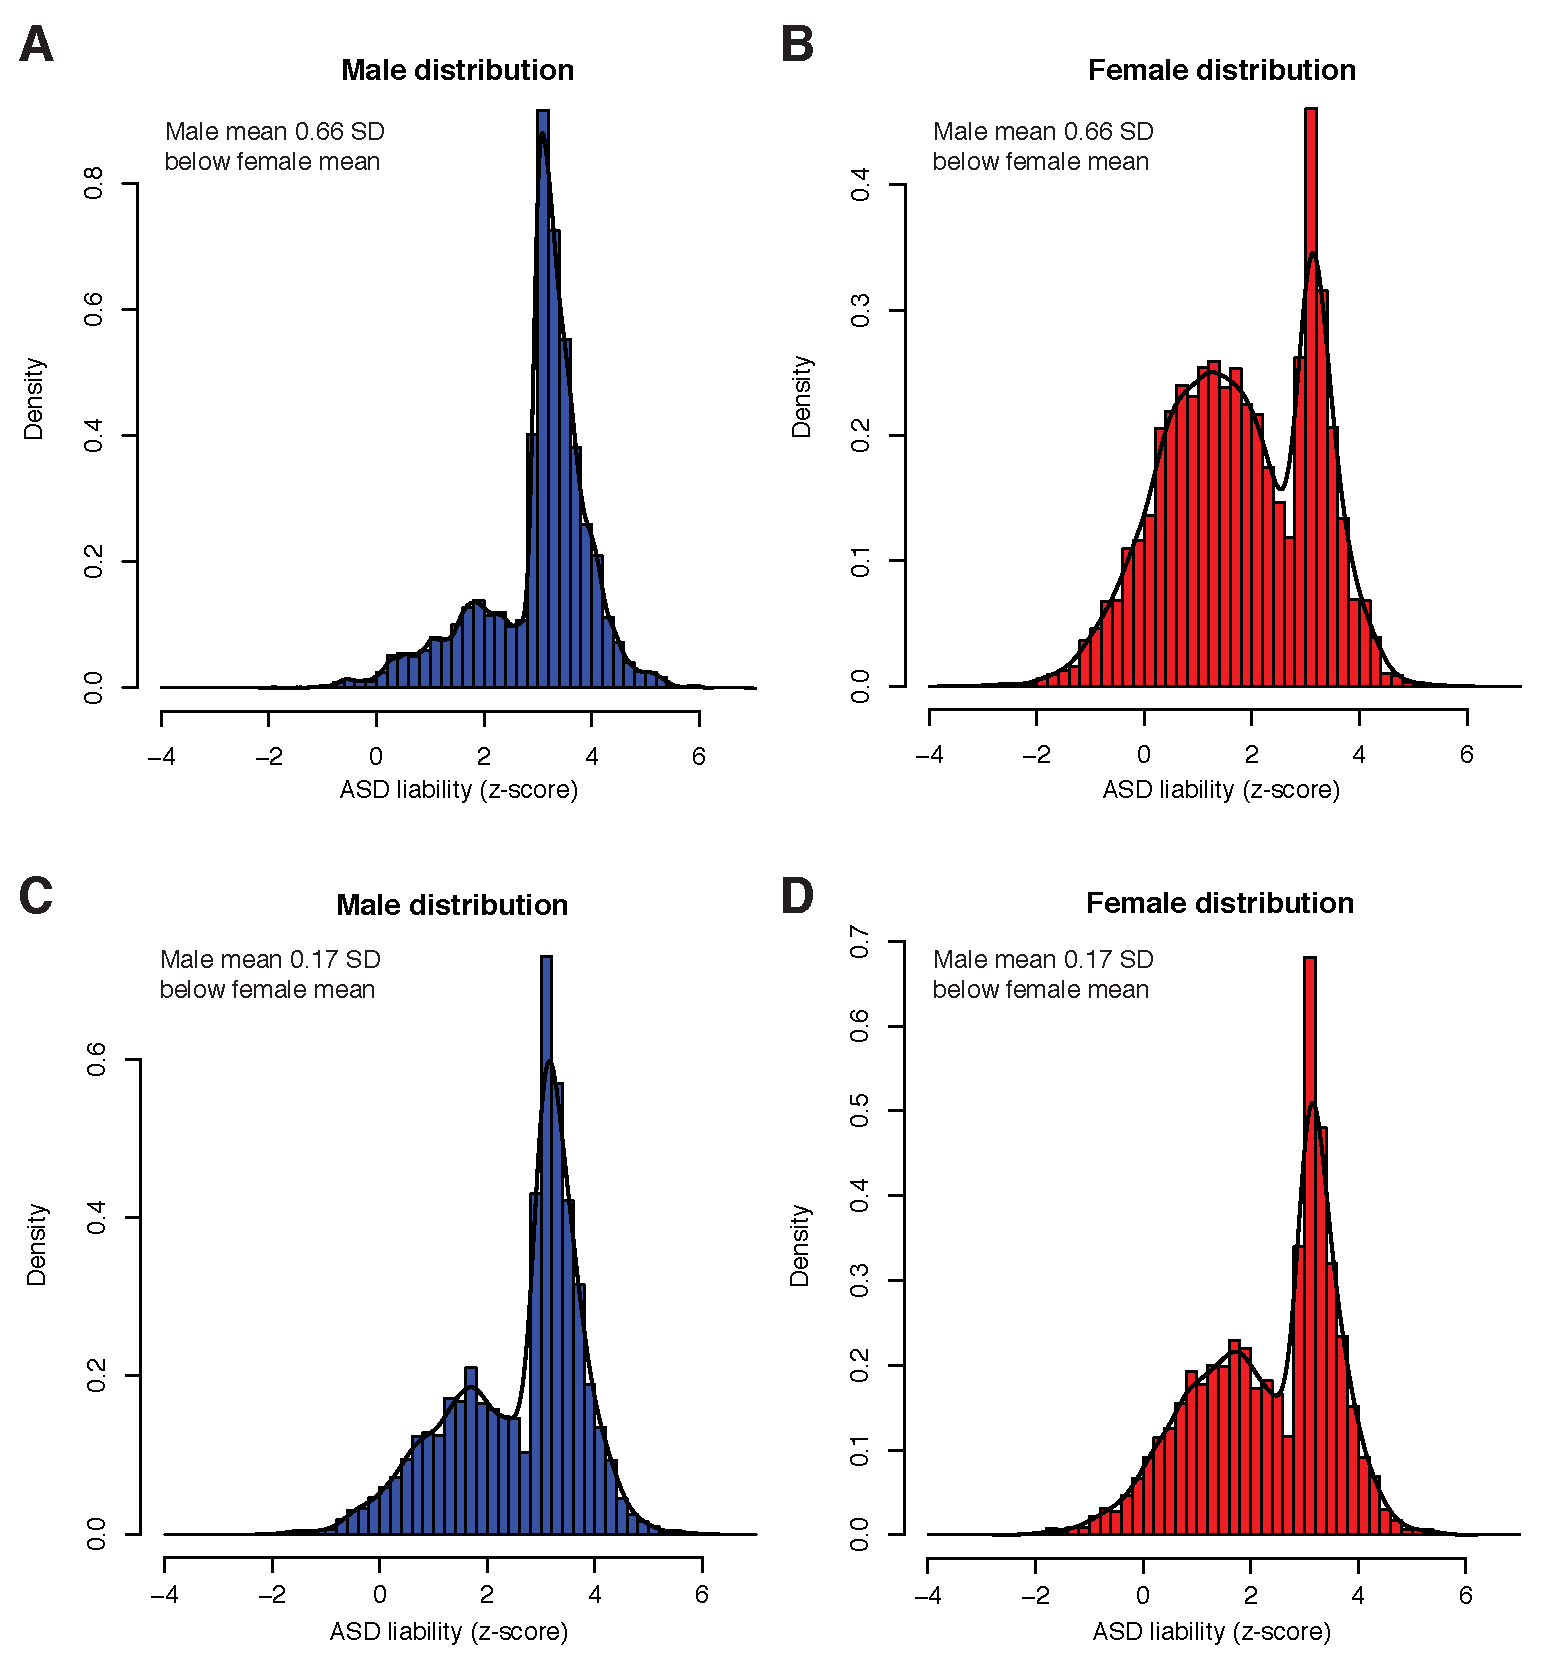
\includegraphics[width=1\linewidth]{Figures/AscertainmentBias.pdf}
		\end{center}
		\caption{\textbf{Effect of Ascertainment Bias on ASD Liability}\label{Figure15}}
		
 		\textbf{A)} Distribution of ASD liability in males in simulated families selected using the ascertainment methods used in the AGRE collection (at least two affected children). The male and female mean liability was shifted by 0.66 standard deviations to give a 4:1 sex bias and the diagnostic threshold was selected to give an incidence of 1\%. \textbf{B)} The female liability distribution under the same model as `A'. \textbf{C)} The simulation was repeated using a shift of 0.17 standard deviations which is equivalent to the difference of 3 SRS points observed between male and female samples. \textbf{D)} The female liability distribution under the same model as `C'.
	\end{figure}
	\clearpage
}\normalsize

\section{Results}
	\subsection{Targeted Association Study: Tier 1 SNPs}
		To test the hypothesis that the FPE is mediated by a common variant at a single locus an association test comparing 208 affected females against 151 unrelated unaffected females was performed. Since the FPE is unique to females, it was reasoned that the region of the genome that has the greatest potential for sexual dimorphism would be the most likely location for such a locus, therefore the first tier of the analysis was performed on 451 SNPs that are unique to chromosome X and that escape X-inactivation (Figure \ref{Figure5} and Table \ref{Table1A}). No SNPs were significant after correcting for the 451 comparisons (Figure \ref{Figure16}). Of the top five SNPs (Table \ref{Table5}), only three had a dominant risk allele that was observed more frequently in the affected females (odds ratio $>$ 1) and none had allele frequencies close to the prediction in both the affected and unaffected groups. Only one of these five SNPs was represented on the microarrays used for the SSC replication cohort (207 affected females, 676 unaffected females); despite this SNP reaching nominal significance, the dominant risk allele was more frequent in the unaffected group, i.e. the opposite direction of effect observed in the discovery sample. Given the targeted nature of this analysis, the estimated power to discover a single locus meeting the hypothesis was 100\% even with modest enrichment of unprotected females in the affected group (Figure \ref{Figure2}).

	\subsection{Targeted Association Study: Tier 2 SNPs}
    
    	Since no clear candidates were observed in the tier 1 SNPs, the analysis was expanded to the whole of chromosome X to account for the possibility that that of regions escaping X-inactivation may not be complete. As with the tier 1 analysis, no SNPs showed significant association after correcting for the 6,955 comparisons (Figure \ref{Figure16}B). Considering the top SNPs (Table \ref{Table6}), all five showed a direction of effect that was the opposite of expectation given the allele frequencies (see Supplemental Methods). None of these SNPs were nominally significant in the SSC replication cohort. Of note, none of the top five SNPs from the tier 1 analysis were in the top five for the tier 2 analysis, despite all 451 tier 1 SNPs being included in this analysis. The statistical power to detect the hypothesized single FPE locus was still estimated to be 100\% for tier 2.
        
     \subsection{Genome Association Study: Tier 3 SNPs}
			
        Next, the possibility that the protective allele was not on chromosome X, (e.g. an autosomal gene that was only expressed in the presence of high estrogen levels) was considered. Therefore the analysis was repeated for all 317,574 SNPs in the AGRE group. Again there was no association after correction for multiple comparisons (Figure \ref{Figure16}C) and none of the top five SNPs were nominally significant in the replication group (Table \ref{Table7}). Of note, none of the top five SNPs were on chromosome X. Even with the larger number of SNPs, we estimated our power to detect the hypothesized single FPE locus to be 100\% (Figure \ref{Figure4}).
            
    \subsection{Exploratory Association Analyses}        
      	
        Finally, the possibility that our inability to detect the hypothesized single FPE locus was due to inaccurate differentiation of females with, and without, the FPE was considered . For instance, a female may be unaffected due to the absence of risk factors despite absent FPE. Therefore cases and controls were defined by their SRS score rather than by categorical ASD diagnoses. No SNPs were significant after multiple comparisons (Figures \ref{Figure8},\ref{Figure9},\ref{Figure10},\ref{Figure11}, and Table \ref{Table4}). Next, whether extremes of the affected and unaffected SRS distributions might be enriched for females in whom the FPE was present or absent was considered (Figure \ref{Figure14}). Again, no SNPs were significant after multiple comparisons (Table \ref{Table4}). In addition, all of the reported analyses were preformed under an additive model; no genome-wide significant SNPs were identified (Figure \ref{Figure12} and \ref{Figure13}, Table \ref{Table8} and \ref{Table9}).
            
\afterpage{
    \begin{figure}[p]
		\centering
		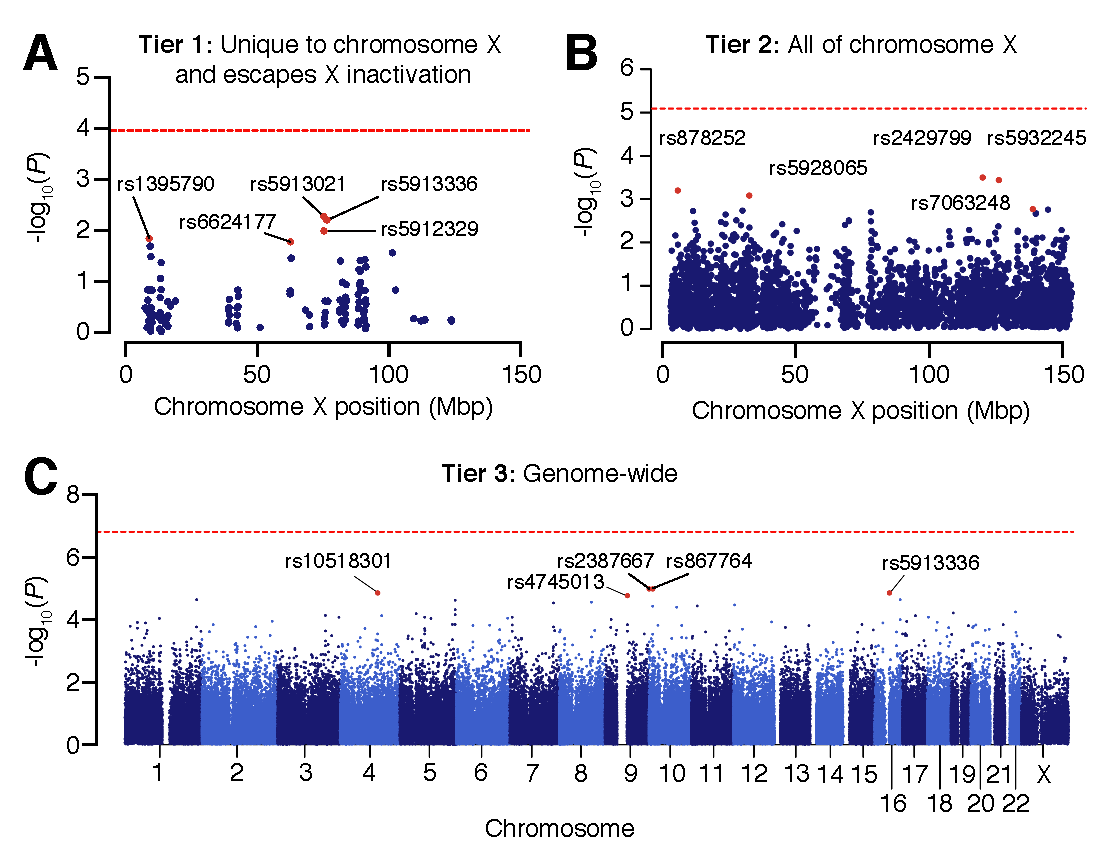
\includegraphics[width=1\textwidth]{Figures/Figure_4_GWAS_Gockley_Dec2014.pdf}
        		\caption{\textbf{Manhattan Plots of Association Study Results.}\label{Figure16}}     	
       		\begin{flushleft}Results of association studies comparing 208 affected females and 151 unaffected females from AGRE. To maximize the ability to identify a candidate variant for the FPE the association test was performed on three tiers of SNPs, based on the a priori probability of mediating the FPE. A) Tier 1: 451 SNPs unique to chromosome X that escape X inactivation. No SNPs are significant after multiple comparisons (horizontal red line). The top five SNPs (red) are labeled (Table \ref{Table1}). B) Tier 2: all 6,955 SNPs on chromosome X. No SNPs are significant after multiple comparisons (horizontal red line). The top five SNPs (red) are labeled (Table \ref{Table2}). C) Tier 3: all 317,574 SNPs across the genome. No SNPs are significant after multiple comparisons (horizontal red line). The top five SNPs (red) are labeled (Table \ref{Table3}). 
       		\end{flushleft}
	\end{figure}
	\clearpage
	}
    \normalsize

\afterpage{
	\scriptsize 
    \begin{table}[p]
		\renewcommand{\arraystretch}{1}
        \centering
        	\resizebox{1.0\textwidth}{!}{%
			\begin{tabular}{ccccccccccc}
					 
				 & \multicolumn{6}{c}{\underline{AGRE Discovery (208 cases, 151 Controls)}} & \multicolumn{4}{c}{\underline{SSC Repplication (207 cases, 676 Controls)}} \\ 
 
\textbf{SNP} 	& Allele 1/ & Aff Allele  & UnAff Allele & Odds  &   P    & Corr P   & Aff Allele  & UnAff Allele & Odds  & P       \\ 
				& Allele 2 & 1 Freq (\%) & 1 Freq (\%)  & Ratio  & Value  & P-Value   & 1 Freq (\%) & 1 Freq (\%)  & Ratio & Value   \\ \hline
Predicted		&          &    97.0     &   $<$24.3    &   $>$88& $\leq1*10^{-8}$&  $\leq0.05$   & 97.0      &  $<$24.3     &$>$88  & $\leq1*10^{-8}$ \\ 
rs5913021 		&  G/A     &    71.5     &     57.3     &   1.25 & 0.005  &  1.0  &               &           &       &         \\ 
rs5913336 		&  A/G     &    49.0     &     63.6     &   0.77 & 0.006  &  1.0  &       69.9    & 60.9      &  1.14 &  0.007  \\ 
rs5912329 		&  A/G     &    71.4     &     58.2     &   1.23 &  0.01  &  1.0  &               &           &       &         \\ 
rs1395790 		&  G/A     &     2.4     &      7.9     &   0.30 &  0.01  &  1.0  &               &           &       &         \\ 
rs6624177 		&  A/G     &    60.0     &     72.2     &   0.83 &  0.02  &  1.0  &               &           &       &         \\ 
			\end{tabular}%
            }
			\caption{\textbf{Top Five SNPs from Tier 1 Analysis}\label{Table5}}
			
	\end{table}
	\clearpage
}\normalsize

\afterpage{
	\scriptsize 
    \begin{table}[p]
		\renewcommand{\arraystretch}{1}
        \centering
        	\resizebox{1.0\textwidth}{!}{%
			\begin{tabular}{ccccccccccc}
					 
				 & \multicolumn{6}{c}{\underline{AGRE Discovery (208 cases, 151 Controls)}} & \multicolumn{4}{c}{\underline{SSC Repplication (207 cases, 676 Controls)}} \\ 
 
\textbf{SNP} 	& Allele 1/ & Aff Allele  & UnAff Allele & Odds   & P      & Corr P   & Aff Allele  & UnAff Allele & Odds  & P       \\ 
				& Allele 2 & 1 Freq (\%) & 1 Freq (\%)  & Ratio  & Value  & P-Value  & 1 Freq (\%) & 1 Freq (\%)  & Ratio & Value   \\ \hline
Predicted		&          &    97.0     &   $<$24.3    &   $>$88& $\leq1*10^{-8}$&  $\leq0.05$   & 97.0      &  $<$24.3     &$>$88  & $\leq1*10^{-8}$ \\ 
rs2429799&  A/G     &    21.2     &      7.3     &   2.90 & 0.0003 & 1.0   &               &           &       &         \\ 
rs5932245&  A/G     &    97.1     &     87.4     &   1.11 & 0.0004 & 1.0   &     54.1      &   55.0    &  0.98 & 0.9645   \\ 
rs878252 &  G/A     &    31.7     &     15.9     &   2.00 & 0.0006 & 1.0   &     29.0      &   25.6    &  1.13 & 0.1699  \\ 
rs5928065&  G/A     &    94.7     &     84.1     &   1.13 & 0.0008 & 1.0   &     88.4      &   93.3    &  0.95 & 0.5674  \\ 
rs7063248&  G/A     &    73.4     &     57.6     &   1.27 & 0.0017 & 1.0   &     97.1      &   96.6    &  1.01 & 0.1885  \\ 									\end{tabular}%
            }
			\caption{\textbf{Top Five SNPs from Tier 2 Analysis}\label{Table6}}
			
	\end{table}
	\clearpage
}\normalsize

\afterpage{
	\scriptsize 
    \begin{table}[p]
		\renewcommand{\arraystretch}{1}
        \centering
        	\resizebox{1.0\textwidth}{!}{%
			\begin{tabular}{ccccccccccc}
					 
				 & \multicolumn{6}{c}{\underline{AGRE Discovery (208 cases, 151 Controls)}} & \multicolumn{4}{c}{\underline{SSC Repplication (207 cases, 676 Controls)}} \\ 
 
\textbf{SNP} 	& Allele 1/ & Aff Allele  & UnAff Allele & Odds   & P      & Corr P   & Aff Allele  & UnAff Allele & Odds  & P       \\ 
				& Allele 2 & 1 Freq (\%) & 1 Freq (\%)  & Ratio  & Value  & P-Value  & 1 Freq (\%) & 1 Freq (\%)  & Ratio & Value   \\ \hline
Predicted		&          &    97.0     &   $<$24.3    &   $>$88& $\leq1*10^{-8}$&  $\leq0.05$   & 97.0      &  $<$24.3     &$>$88  & $\leq1*10^{-8}$ \\ 
rs2387667 &  G/A     &    33.7     &     13.2     &   2.54 & $1.1*10^{-5}$ &  1.0  &    15.9       &   19.5    &  0.82 & 0.25    \\ 
rs867764  &  A/G     &    33.7     &     13.2     &   2.54 & $1.1*10^{-5}$ &  1.0  &    23.2       &   23.5    &  0.99 & 0.92    \\ 
rs10518301&  A/G     &    25.0     &     47.0     &   0.53 & $1.4*10^{-5}$ &  1.0  &    40.1       &   41.1    &  0.98 & 0.79    \\ 
rs9302760 &  A/G     &    75.0     &     53.0     &   1.42 & $1.4*10^{-5}$ &  1.0  &    60.4       &   56.4    &  1.07 & 0.31    \\ 
rs4745013 &  G/A     &    36.1     &     58.9     &   0.61 & $1.7*10^{-5}$ &  1.0  &    49.8       &   47.8    &  1.04 & 0.62    \\ 
			\end{tabular}%
            }
			\caption{\textbf{Top Five SNPs from Tier 3 Analysis}\label{Table7}}
			
	\end{table}
	\clearpage
}\normalsize

%%Additive Model SNP table - AGRE
\afterpage{
	\renewcommand{\arraystretch}{1}%
	\begin{table}[p]
		\begin{center}
			\begin{tabular}{cccccc}

				Comparison&SNP&Chr&Position&P-Val&BF-Corrected\\		
				\hline													
				\\

				%%Afected vs Unaffected
				& rs1028348 & X & 65384163 & 1.7E-03 & 0.77 \\
				Affected & rs670546 & X & 65272116 & 3.3E-03 & 1 \\
				Versus & rs5965083 & X & 65230426 & 3.6E-03 & 1 \\
				Unaffected & rs5964488 & X & 65253769 & 4.9E-03 & 1 \\
				& rs6525038 & X & 65193018 & 6.7E-03 & 1 \\
				\hline													
				\\

				%%High low SRS
				& rs7891218 & X & 92952292 & 2.0E-03 & 0.91 \\
				High SRS & rs5983514 & X & 92674286 & 7.9E-03 & 1 \\
				Versus & rs1409117 & X & 53302495 & 8.4E-03 & 1 \\
				Low SRS & rs2146335 & X & 44504859 & 8.6E-03 & 1 \\
				 & rs7050908 & X & 45033139 & 1.0E-04 & 1 \\
				\hline													
				\\	

				%%GWAS
				& rs7668302 & 4 & 29852055 & 4.8E-07 & 0.15 \\
				& rs4745013 & 9 & 72277423 & 1.1E-06 & 0.34 \\
				GWAS & rs867764 & 10 & 12794868 & 1.2E-06 & 0.38 \\
				& rs7020846 & 9 & 28393443 & 1.8E-06 & 0.56 \\
				& rs9943244 & 1 & 15268468 & 4.8E-06 & 1 \\
				\hline													
				\\	

			\end{tabular}
			\caption{\textbf{Top SNPs from Additive Model Analysis of the AGRE Cohort}\label{Table8}}
			
		\end{center}
	\end{table}
	\clearpage
}\normalsize

%%Additive Model SNP table - SSC
\afterpage{
	\renewcommand{\arraystretch}{1}%
	\begin{table}[p]
		\begin{center}
			\begin{tabular}{cccccc}

				Comparison&SNP&Chr&Position&P-Val&BF-Corrected\\		
				\hline													
				\\

				%%Afected vs Unaffected
				& rs6621080 & X & 100630202 & 3.2E-03 & 1 \\
				Affected & rs845127 & X & 7785325 & 3.4E-03 & 1 \\
				Versus & rs5979883 & X & 13390855 & 4.0E-03 & 1 \\
				Unaffected & rs7058967 & X & 44592534 & 4.1E-03 & 1 \\
				& rs16984793 & X & 7815994 & 5.3E-03 & 1 \\
				\hline													
				\\

				%%High low SRS

				& rs5979883 & X & 13390855 & 2.7E-03 & 0.91 \\
				High SRS & rs7058967 & X & 44592534 & 5.5E-03 & 1 \\
				Versus & rs845127 & X & 7785325 & 6.3E-03 & 1 \\
				Low SRS & rs12846943 & X & 44607553 & 8.9E-03 & 1 \\
				& rs6621080 & X & 100630202 & 9.2E-03 & 1 \\
				\hline													
				\\	

				%%GWAS
				& rs1454870 & 4 & 11884740 & 7.3E-06 & 1 \\
				& rs12462380 & 19 & 16298048 & 7.7E-06 & 1 \\
				GWAS & rs1054227 & 6 & 100097577 & 1.0E-05 & 1 \\
				& rs2296154 & 6 & 100099989 & 1.1E-05 & 1 \\
				& rs2124141 & 4 & 11851124 & 1.6E-06 & 1 \\
				\hline													
				\\	

				\end{tabular}
			\caption{\textbf{Top SNPs from Additive Model Analysis of the SSC Cohort}\label{Table9}}
			
		\end{center}
	\end{table}
	\clearpage
}\normalsize

	\section{Discussion}

	The observation of a bimodal SRS distribution in females, but not males, from multiplex families raised the possibility of a single genetic locus mediating a female protective effect and resulting in a 4:1 sex bias in ASD. Given the potential of such a locus as a therapeutic target, and the high likelihood that such a locus would be missed by a GWAS with mixed sexes, this association study, which was well powered to detect such an effect was preformed.
	\par Three tiers of SNPs were considered, these were based on the a priori probability that genomic regions might harbor a single locus for FPE. The first tier considered only SNPs unique to chromosome X that escaped X-inactivation, the second tier considered all SNPs on chromosome X, and the third tier was a full genome-wide association study. No SNPs reached significance after correcting for multiple comparisons in any of the three tiers (Figure \ref{Figure16}); furthermore there was no evidence of replication in the SSC cohort, nor of a SNP in one tier being present in the top five SNPs of the next tier. This result was unchanged by an additive model (Figure \ref{Figure12} and \ref{Figure13}), defining case/control status using the SRS score (Figures \ref{Figure14}, Table \ref{Table4}), or considering the extremes of the SRS distribution (\ref{Table4}). 
	\par The female-only GWAS achieved considerably higher power than a GWAS with both sexes and was extremely well powered to detect a single locus for the FPE even with marked deviation from the expected allele frequency (Figure \ref{Figure4}). Therefore it can be concluded that the FPE is unlikely to be mediated by a single genetic locus. This negative result does not reduce the likelihood of a female protective effect being responsible for the sex bias observed in ASD, nor does it reduce the likelihood of this protection being mediated by a polygenic effect. 
	\par There are several explanations for this negative result. First, there may be little variance in the FPE between females. For example, if the FPE was mediated by endogenous estrogen levels above a certain threshold, and all females exceeded this threshold, then the FPE would be constant without genetic or environmental risk factors having an effect.Recent evidence after this work was published points to a potential mechanism of estrogen mediated rescue of potential ASD behavior in zebra fish\cite{Hoffman:2016aa}. Alternatively, the FPE may vary between females, but this variance is determined by multiple genetic and/or environmental factors, for example if the extent of FPE was dependent on the degree of endogenous estrogen exposure. Finally, it is possible that a single environmental factor (e.g. exogenous estrogen exposure) determines the presence of the FPE, though such a factor would need to act in the majority of females, but not act in the majority of males.
	\par The first explanation (FPE in all females) would not lead to the bimodal SRS distribution that prompted this study (Figure \ref{Figure1}H), while the second (multifactorial FPE) could only produce a bimodal distribution if the majority of risk factors targeted a common biological pathway or neurological process (Figure \ref{Figure1}F). It is hard to reconcile the third explanation (a single environmental effect) with the consistent sex bias observed across so many studies. 
	\par This leads towards considering alternative explanations for the bimodal distribution. Firstly there's the consideration of ‘non-biological’ biases in the manner of data collection. One possibility is ascertainment bias, i.e. that unaffected males are rare in multiplex families, while unaffected females are detected comparatively frequently. Simulation of multiplex families shows that ascertainment bias and a 4:1 sex bias can induce a bimodal distribution in ASD liability that is more pronounced in females (Figure \ref{Figure15}A and \ref{Figure15}B). However, this is most likely not the complete explanation of the SRS distribution since the observed data differs from the expectation of this model in two important respects: 	
	\par First, the lower distribution in females (Figure \ref{Figure15}B) has a mean over one standard deviation above the general population (equivalent to an SRS score of over 40). However, in the multiplex females (Figure \ref{Figure1}B) the lower distribution females is the same as the general population (SRS of 18). 
	\par Second, the simulation required a difference in mean liability between males and females of 0.66 standard deviations (equivalent to an SRS of 12). However, the observed SRS difference between males and females is four-fold lower at 0.17 standard deviations (equivalent to an SRS of 3). If the simulation is repeated using a sex difference of 0.17 standard deviations we observe little distinction between the male and female distributions (Figure \ref{Figure15}C and \ref{Figure15}D). 
	\par Therefore, while ascertainment bias may partially explain the bimodal SRS in multiplex females, these analyses suggest it is not the complete explanation of this phenomenon. Similarly, the effect may be a consequence of the sex of the parent rating the child for the SRS score. However, no such rater bias was detected in epidemiologic sample of twins\cite{Constantino:2003aa,Constantino:2005aa} and the bimodal distribution has been observed for SRS scored by both parents and teachers\cite{Virkud:2009aa}. Finally, it was considered whether IQ could confound the SRS score, however, only a very weak correlation between the two measures with a similar slope in males and females was observed(Figure \ref{Figure17}).
	\par Next ‘biological’ explanations for the bimodal distribution were considered. The ‘single locus’ observed may represent a rare risk factor rather than a rare protective factor, e.g. inherited large copy number variation (CNV). The distribution may also be a consequence of more complex interactions between multiple factors mediating protection and risk. For example, a general population twin study\cite{Constantino:2003aa} observed that reciprocal social behavior in females, but not males, was influenced by rearing factors that operated in the direction of promoting social competency. Further exploration of the manner in which inherited liability to ASD might capitalize upon, or accentuate, developmental sexual dimorphisms in gene expression, neuroanatomy, or behavior are warranted. It is of note that a large family study\cite{Constantino:2010aa} observed that a high proportion of the unaffected sisters of ASD probands manifested histories of early language delay with autistic qualities of speech which later resolved. These observations offer potential clues to the manner in which FPE might offset risk in the setting of autism susceptibility early in life.
	\par Microarray and exome sequencing studies have observed an excess \textit{de novo} mutation burden in ASD affected females compared to ASD affected males\cite{Dong:2014aa,Jacquemont:2014aa,Sanders:2011aa,Levy:2011aa}; however a quantitative relationship was not observed between CNV trait burden and ASD symptom severity. This underscores the possibility that FPE operates in a dichotomous manner, either offering complete protection from ASD risk or being completely overwhelmed by an excess of ASD risk.
	\par In summary, the distribution of ASD severity in females raised the possibility of an ASD protective effect in females mediated by a single genetic locus. If present, such a locus is likely to have been missed by prior GWAS analyses and would have great potential as a therapeutic target. However, this study represents a well-powered targeted association that found no evidence of such a genetic locus. The FPE remains of great interest as a route to discovering therapeutic targets, however the mechanism of this protection remains unknown. 

\afterpage{
	%%IQ vs. SRS
	\begin{figure}[p]
		\begin{center}
			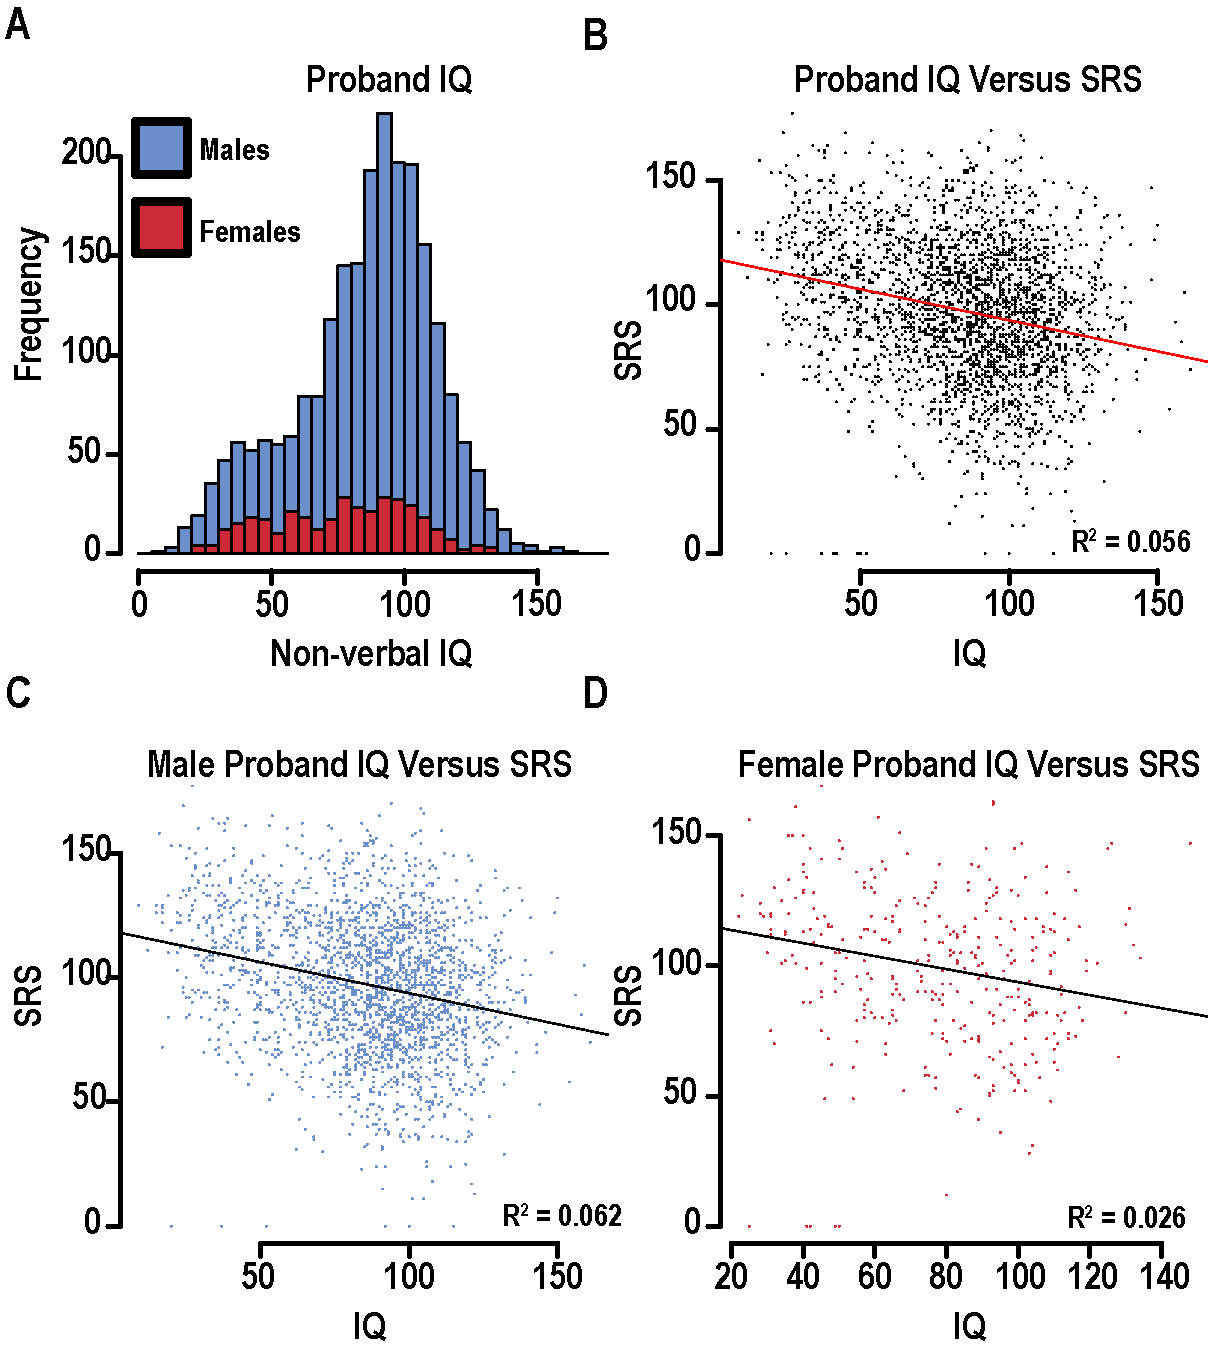
\includegraphics[width=1\linewidth]{Figures/IQv2.pdf}
		\end{center}
		\caption{\textbf{IQ Distribution in SSC Probands}\label{Figure17}}
		
		\textbf{A)} Histogram of male (blue) and Female (red) IQ distributions in SSC probands. \textbf{B)} Plot of SRS as a function of IQ in SSC probands. Linear regression model was used to generate the best fit line (red) and correlation value (R\textsuperscript{2}). \textbf{C)} Plot of SRS as a function of IQ in male SSC probands. Linear regression model was used to generate the best fit line (red) and correlation value (R\textsuperscript{2}). \textbf{D)} Plot of SRS as a function of IQ in female SSC probands. Linear regression model was used to generate the best fit line (red) and correlation value (R\textsuperscript{2}).
	\end{figure}
	\clearpage
}\normalsize

\chapter{Cis-Regulatory Space, a Genomics Evolutionary Toolkit}
	\section{Background}
    	%\setlength{\parindent}{10ex}\par
		

\textit{What Defines Humans from the Animal Kingdom?}\par \bigskip

	The question above has been answered dozens of ways and yet never solved. An anthropological viewpoint highlights the mass domestication of plants and animals into agrarian culture, as a clear delineation between us and other primates. An engineering based explanation would highlight our high dexterity allows for fine manipulation, empowering the advanced tool making capability that is vital to agrarian development. Linguists and anthropologists would highlight the expansion of language comprehension and synthesis structures in the brain, which allow for complex speech formation aiding the expansion our functional societal unit size relative to our closest ancestors\cite{DUNBAR:1993aa}. A more behavioral approach would posit that the capacities of imitation, deception, and theory of mind define us. While all of these responses contain a certain necessity required of defining humanity, alone neither is sufficient to entirely answer the question.\par 
The answers above all highlight the differences between us and the animal kingdom, in particular our closest ancestors, as the definition of what being human is; therefore the sufficient answer should encompass the foundation of all the above. 
As the genome is foundational unit encoding the entirety of information required developing an organism; differences between human and non-human primate genomes are a natural place to start. \par

	\subsection{Genomic Sequence Conservation}

	While the answer may lie in genomic differences, the human genome is highly similar to closely related primate and more distantly related mammalian species. The chimpanzee genome is over 99\% similar to human\cite{Chimpanzee-Sequencing-and-Analysis-Consortium:2005aa}. Mice, a far more divergent organism that chimpanzee, have a genome to which 40\% of the human genome can be directly aligned\cite{Mouse-Genome-Sequencing-Consortium:2002aa}. This infers that the divergent portion of genome, likely to be responsible for human specific attributes, is relatively small; while the rest of the genome contains either no function or conserved function. Given this reduced window of interrogation it would be easy, and incorrect, to assume that the underlying human specific genetic foundation would be straightforward to identify. A vital capacity of the genome is the ability to create a vast array of tissues, containing dozens to thousands of different cell types from the information coded within the same genomic unit.\par 

	\subsection{Species Brain Morphology Comparison}

	To reduce inquiry from the entirety of tissue and cell type combinations, application of the adage ‘structure dictates function’ to the previous explanations would narrow the space of investigation to a smaller cohort of structures, one of which is the human brain. The brain plays a vital underlying role in human specific behavior, language, and cognitive performance. As an initial observational pass differences in structure, assuming these changes underlie differential function, could be leveraged to identify orthologous regions of the genome which function differently between species. The human brain is three times larger than gorilla or chimpanzee; normalized by body mass humans have by far the largest brain to mass ratio of all primates\cite{Roth:2005aa}. However, by this definition alone, other mammals such as the shrew and mouse would have far greater neural capacities. Focusing on the cortex, as the rapid expansion of the cortex has been implicated in increased cognitive performance\cite{Fjell:2015aa}. The 2875x increase in the number of cortical neurons in humans compared to mice would infer that the amount of cortical neurons would explain increased cognitive capabilities\cite{Roth:2005aa}. By this measure elephants and whales would cognitively similar to humans, despite total brain weight being 3-4x as large. Incorporation of these factors point to the increased neuronal density as being a fundamental measure, and would allow higher degrees of connectivity within the brain. A parallel measure, the encephalization quotient, delineates humans more clearly than the total brain mass or amount of cortical neurons across all mammals while also being order of magnitude higher in humans relative to non-human primates and 6-9x the size of Rhesus Maquac\cite{Roth:2005aa,Dorus:2004aa}.\par
	
    If the highly expanded cortex in humans is the key underlying structure of human cognitive capabilities, the differences in structure relative to closely related primates as well as mammals should underlie some portion of the differential cognitive function, which we designate as fundamental to human specific behavior. The primate cortex is heavily expanded in primates relative to most mammals, with the cortical plate and sub-plate\cite{Dehay:2007aa}. While within primates there are differences in cortical thickness, a much more pronounced change in cortical volume sets great apes and in particular humans apart. This increase in volume and surface area allows for a ten-fold increase in the amount of discrete functional areas within the human cortex compared to early mammals\cite{Kaas:2013aa}. Along with this expansion in volume, the density neurons within the cortex in primates has increased dramatically accompanied with a steeper rostral-caudal gradient of neuron density\cite{Finlay:2015aa}. These changes in developed morphology correlate to increased cognitive capacity in primates versus mammals as well as between humans and  primates\cite{Fjell:2015aa,Kaas:2013aa,DUNBAR:1993aa,Finlay:2015aa,Roth:2005aa}. Considering this, the underlying developmental mechanisms of this morphology are key to understanding the origin of functional genetic differences between humans and our closest ancestors. 

\subsection{Cortex Development}

The fundamental developmental zone of the cortex is at the base of the developing cortex in the ventricular zone (VZ). Within this zone neural progenitor cells symmetrically divide to create the population of cells, which will give rise to the six-layer cortex above. This neuronal progenitor population becomes particularly large in mammals is additionally represented in the above Sub-Ventricular Zone (SVZ)\cite{Molnar:2006aa}. This added capacity may aid in generation of  a larger proportions of GABAnergic neurons as humans develop 65\% of their GABAnergic neurons in the cortical germinal zones while mice only generate 5\%\cite{Molnar:2006aa}. The rest migrate tangentially into the SVZ from the telencephalon\cite{Bystron:2008aa}. While the increase of a progenitor population explains the increase in neurons of humans relative to other primates the relative increase in surface area versus thickness between humans and primates lies in conserved function.\par
The cortex exhibits radial growth once neurogenesis begins from asymmetrical division of neuroprogenitor radial glial cells. Neurons migrate radially along the radial glial cells to form the cortex from the inside out starting with the deep layer VI and ending with the upper layers II/III\cite{Schwartz:1991aa}. This migration is carefully timed and guided from below by the radial glial progenitors as well as from above where Cajal Retzius Cells, which reside above the developing cortex in the marginal zone and secrete reelin, a signaling molecule which guides layer formation of radiating neurons\cite{Molnar:2006aa,Dehay:2007aa}. This model, the radial unit hypothesis, combined with cellular division of these radial progenitors not only increases the number of neurons, but also the density of cortical units. This increase in units would cause a much faster expansion of cortical volume relative to density, both trends exhibited in humans compared to great apes\cite{Rakic:2009aa}. Increasing the amount of cortical units also allows the addition of more cortical functional regions as, cortical columns can differ in neuronal type and connectivity to form discrete areas\cite{Rakic:2009aa}. Fewer than 7 more rounds of symmetrical division in cortical progenitor populations within the VZ would explain the 1,000 fold expansion of surface area between humans and mice\cite{Rakic:2009aa}. Understanding the underlying genetic foundation of these specific processes, which drive the morphological changes in humans relative to our closest ancestors, is vital towards understanding evolutionary mechanisms\cite{Geschwind:2013aa}.\par 

	\subsection{Evolution of Cis-Regulatory Elements as a Mechanism of Morphological Change}

The source of these changes in the human cortex has proven elusive. The preliminary target of inquiry was in the genic coding sequences of the human genome, in particular a brain-expressed genes. Genic sequences are a problematic target for several reasons; the primary issue is one of pleiotropy. Many genes function across developmental time and tissue domains, making a necessity of any coding alteration to either not carry a detriment to other processes, or affect a motif which only functions in a single tissue and time point\cite{Stern:2000aa}. This is specifically important in developmental genes which tend to be highly conserved\cite{Burke:1995aa}. The rate of evolution of brain expressed genes in humans compared to other primate and mammals, with the exception of one study\cite{Dorus:2004aa} are strongly suspected to have a much slower rate of evolution than both genes expressed specific to and between tissues\cite{Wang:2007aa}. This is despite the fact that tissue specific genes tend to evolve more rapidly than non-tissue specific genes\cite{Duret:2000aa}. This is not to discount the evidence that there are a handful of rapidly evolved brain expressed genes\cite{Evans:2004ab,Evans:2004aa,Burki:2004aa}, however the vast amount of differences can’t be explained by these genes alone. Supporting this notion, is the fact that over two thirds of sequences in the human genome under purifying selection are non-protein coding\cite{Carroll:2005aa,Mouse-Genome-Sequencing-Consortium:2002aa}. Looking broadly between C. Elegans and humans, each of which have 20,000-25,000 genes, it would be difficult to assume that the same size set of genes alone were the only effective genomic input creating the ~1,000 cell types in C. Elegans and trillions of cell types in humans\cite{Bulger:2011aa}. There must be mechanisms directing tissue specificity which would represent ideal targets to modify the development of specific tissues or subsets of cell types.\par
	
    It has been a long standing hypothesis that altering the mechanisms controlling gene expression rather than function of its corresponding protein function is a major driving force of tissue specific evolution\cite{King:1975aa}. While the lack of significant functional sequence divergence in protein coding space may have given rise to this hypothesis, only recently have inroads been made into understanding the full concert of gene expression mechanisms. This space is largely dominated by cis-factors such as enhancers and promoters, trans-factors such as transcription factors and, genomic architecture scaffolding proteins like cohesion. This creates the logical conundrum of the chicken and the egg; what effects expression more, the trans-factor environment driving expression or the sequences that recruit the trans-factors to discrete genomic intervals? While this is question alone could fill a space far larger than can be dedicated here, there are a few key studies that examine this question in a purely evolutionary sense. The first is an elegant study from Wilson and colleagues which leveraged an aneuploid mouse model for trisomy 21 containing either human or mouse chromosome 21. They found that the vast majority of trans-factor binding events on the chromosome in the mouse model resembled those exhibited in the species of origin. Gene expression across the chromosome was also highly correlated to the species of origin despite existing in the mouse trans-environment\cite{Wilson:2008aa}. A more balanced approach employed by Wittkopp and colleagues examined sterile F1 hybrids of two closely related fruit fly species. Of 29 differentially expressed genes 28 were found to have differences in cis-regulation, while 16 had differences in trans-factor regulation. This study illustrates the power of cis-regulatory changes on evolution while also illustrating the complementary or antagonistic roles of trans-environmental factors which also show specificity between tissues\cite{Wittkopp:2004aa,Schmid:2012aa}. While these studies elucidate the ability of cis-regulatory changes to direct spatio-temporal expression though evolutionary timespans, they require a more direct connection to evolutionary and developmental phenotypes, including a mechanistic description, to be attributed to the rapid expansion of the human cortex\cite{Wittkopp:2004aa,Wilson:2008aa,Odom:2007aa,Bulger:2011aa}.\par
	
    Initial studies have revealed the impact of cis-regulatory changes affecting targeted change on developmental processes through evolutionary time. Preliminary studies in C. Elegans and drosophila revealed multiple cis-regulatory regions controlling patterning and pigmentation\cite{Ruvkun:1991aa,Wittkopp:2002aa,Wray:2007aa}. Within vertebrates, multiple loci in 3 and 9 spine sticklebacks reduce pelvic spine development when populations immigrate to fresh water habitats\cite{Shapiro:2004aa,Chan:2010aa}. In humans, a long range enhancer of the Sonic Hedge Hog gene (Shh), has been implicated in preaxial polydactyly\cite{Lettice:2003aa}. Shh is a highly conserved gene pivotal in the development and patterning of multiple structures including the limb and nervous system. While these studies illustrate the how cis-regulatory elements control highly conserved developmental pathways across small evolutionary windows, resolution of the mechanisms surrounding cis-regulatory element evolution are beginning to be elucidated.\par

	\subsection{Mechanisms of Cis-Regulatory Evolution}

	The three primary mechanisms for altering cis-regulatory control of genic expression are, exaptation, modification, and deletion. The latter of which is naturally harder to examine as far as affect size, however some studies have identified conserved regions in mammals that are deleted in humans, inferring that deletion of cis-regulatory elements could be a mechanism of speciation\cite{Wittkopp:2011aa,McLean:2011aa}. Exaptation of regulatory elements via translocation has been a long-standing theory of how a regulatory element present in a different region of the genome inserted into a new genomic region and as a result, it’s activity could be co-opted into a different tissue or time point of development based on the local activity of it’s new genomic interval\cite{Britten:1971aa}. While there is debate on the extent of translocation mediated exaptation it does appear to be a viable mechanism of altering cis-regulation of specific gene expression programs over evolutionary time\cite{Emera:2016aa,Kunarso:2010aa}. Modification of a cis-regulatory element would act through mutation of individual bases and result in altering it’s fundamental properties. For example mutations within a transcription factor binding motif could alter its activity and capacity to drive gene expression\cite{Wittkopp:2011aa}. The classic example of a candidate regulatory undergoing modification is the clustered mutation of conserved bases within a highly conserved interval. Interrogation of these regions can yield resolution on extremely recent evolutionary events such as the human-specific gain of function in a highly accelerated conserved sequence (HACNs) by Prabhakar and colleagues\cite{Prabhakar:2008aa}. These mechanisms represent fundamental changes in regulatory elements, however in order to interrogate them on a high throughput and spatio-temporal level techniques besides sequence comparisons are necessary.\par

	\subsection{Mapping Active Regulatory Elements}

	Chromatin-immuno precipitation (ChIP) can identify active enhancers in a tissue dependent manner based on the modification context of associated histones and trans-factor binding proteins. Genomic DNA likely to be active is accessible to the trans-environment and therefore likely to be associated with histones carrying the specific histone destabilizing modifications H3K27ac and H3K4me2/H2K4me3\cite{Ernst:2010aa,Ernst:2011aa}. In addition to histone marks, direct immune-precipitation of trans factors associated DNA can yield maps of active regulatory sequences\cite{Visel:2009aa}. Immuno-precipitation of proteins establishing domain boundaries, such as choesin\cite{Hadjur:2009aa},  can identify large regulatory units or if cross-linked intra-molecularly after precipitation can resolve specific enhancer-promoter interactions\cite{DeMare:2013aa}. Enrichment of genomic DNA cross-linked with these specific histones via antibody purification has proven a successful tool in building tissue specific candidate enhancer maps\cite{Cotney:2012aa}. Aggregation of multiple ChIP-Seq data sets along with gene expression and sequence conservation can improve resolution, yield more accurate predictions of gene targets for regulatory elements, and resolve cell type identity and developmental stage\cite{Visel:2013aa,Zhu:2013aa}. Recently this technique has been leveraged in matched tissues across multiple development stages in human, mouse, and rhesus macaque has yielded insight into sequences exhibiting a gain of H3K27ac and H3K4me2 in humans. This approach has mapped candidate human lineage enhancer gains in the developing limb\cite{Cotney:2013aa} and brain\cite{Reilly:2015aa}. Coupled with the evolutionary evidence from drosophila and mouse studies, the predicted driver of this activity change would be sequence changes within and surrounding the enhancer regions can affect chromatin state {Wilson:2008aa,Wittkopp:2004aa,Schmid:2012aa }. On a mechanistic level, these changes could act through altering association with chromatin assembly proteins such as deacetylases and methyltransferases, or transcription factors. Changing a sequence’s trans-factor associations is a recent hypothesis to explain species specific of chromatin states at discrete loci\cite{McVicker:2013aa}. Candidate maps identifying species-specific chromatin states therefore provide a tantalizing target for functionalization, however high-throughput functionalization remains a challenging prospect in the field of genomics.\par

	\subsection{Functionalization of Regulatory Elements}

    Recently, self-transcribing active regulatory region sequencing (STARR-Seq) and massively parallel reporter assays (MPRAs) have emerged as two promising techniques in which a candidate enhancer’s capacity to drive transcription of a target gene product can be functionalized in a high-throughput fashion. Both techniques read out transcriptional output of transiently transfected, high coverage plasmid libraries containing the library of sequences to be functionally interrogated. The primary differences between the methods are in the molecular schematic of the reporter construct. The candidate reporter/enhancer element (CRE) is self-contained in the un-translated 3’ tail in STARR-Seq, where as the CRE is directly upstream of the promoter and a 12-20bp tag is contained in the 3’ un-translated transcript tail, which corresponds to the specific. The differences in diagnostic read outs between these systems is that STARR-Seq requires a pile-up of CRE reads over input plasmid library (similar to ChIP-Seq), where the MPRA is a direct counts based analysis of tags between plasmid input and transcript fractions. Both methods have been proven to yield interesting insights on regulatory space, yet each have distinct fundamental drawbacks\cite{Babbitt:2015aa}.\par
	
    STARR-Seq has shown promise in being able to functionalize CREs across tissue types and closely related species. Initial STARR-Seq assays were preformed in drosophila and were highly sensitive. Utilizing sonicated fragments of approximately 300bp in length as the input CRE library cloned into the STARR-Seq vector, Arnold and colleagues were able to functionalize enhancer activity across different tissue types with a high dynamic range\cite{Arnold:2013aa}. Furthermore, genome wide functionalization of recently divergent drosophila species yielded species specific enhancer maps created unbiased from sequence conservation selecting for adaptive evolutionary forces\cite{Arnold:2014aa}. Incorporation of this functional readout with other genomics data such as ChIP-seq and sequence conservation can be used to further predict differential CRE activity in a wider array of species\cite{Naval-Sanchez:2015aa}. While initially promising, STARR-Seq has some severe limitations when applied to mammalian genomes. The size of the human genome presents challenges in representative library preparation, amount of transfected cells required, depth of sequencing required, and finally steric difficulties arising from the molecular transcriptional schema. These difficulties will be elucidated further within, but in summation they have limited this technology to highly reduced representation libraries\cite{Vanhille:2015aa}.\par
	
    MPRA has shown highly robust power to quantitate CRE activity. By using synthetic oligos as input, MPRAs can directly compare functional differences of sequence motif changes in regulatory space in both synthetic and biological contexts. This has allowed for the systematic dissection of an individual enhancer, both by showing the allele effect size of individual base changes, and the combinatorial effects of multiple base pair changes contribute to transcriptional output\cite{Melnikov:2012aa}. By examining the individual unit sized activity of an enhancer across steps as small as 5bp\cite{Ernst:2016aa}. MPRA has shown promise in identifying functional variants in the human genome with high resolution\cite{Tewhey:2016aa,Ulirsch:2016aa}, as well as species-specific functional differences\cite{Doan:2016aa}. Initial attempts to assay MPRA libraries in vivo have yielded some promising results as well\cite{Patwardhan:2012aa,Smith:2013aa}. The drawbacks of this method however, lie in the necessity of oligo synthesis input and the high tag redundancy to drive reproducibility. The initial limitation of synthesis lies in sequence length restrictions limiting fragment size to 170bp, below the size of many enhancers. While elegant sub-assembly approaches from Hiatt and colleagues illustrate how to circumvent the size restriction, this only increases the issue of scale, as oligo synthesis remains impracticable to investigate larger regions in a high-throughput\cite{Hiatt:2010aa}. Further restricting the capacity of MPRAs, is the necessity of tag redundancy to ensure high reproducibility, which raises the fundamental sequencing complexity of the library over twenty-fold. This difficulty is best resolved when comparing the sequencing necessary to read the output of an MPRA library to the depth required of differential RNA-Seq experiments. Each input CRE essentially represents a gene in RNA-Seq, increasing the amount of CREs very quickly raises the requisite depth of sequencing necessary to call differential activity to impractical levels. In addition, gaining high count reproducibility at the tag level requires a sequencing coverage 10-100 fold greater. Despite these restrictions, MPRAs remain a highly viable assay to interrogate carefully curated fragment sets for specific functional description of regulatory activity.

\section{Introduction:}
	Enhancers modulate transcription of specific targets throughout development. Enhancer activity is extremely heterogeneous between tissues, and temporally through development\cite{Cotney:2012aa,Zhu:2013aa}. Recently, chromatin mapping of marks denoting active enhancer regions in stage matched tissues of human, rhesus, and mouse has yielded genome wide identification of candidate human-specific enhancer gains in limb\cite{Cotney:2013aa} and brain\cite{Reilly:2015aa}. What these data sets require is functional interrogation to quantify the capacity for these inferred species specific enhancers to drive transcription. Given the size of these data sets, such a method of fictionalization requires high-throughput. Two approaches were taken through development of 2 different technologies, STARR-Seq and MPRA.
	
    \subsection{STARR-Seq:}
    
	STARR-Seq is a high-throughput enhancer assay that utilizes the ratio of transcripts from a self-transcribing DNA fragment to its plasmid template copy number in order to identify sequences that drive transcription. The interrogated DNA fragment is self-contained within the transcript, making this a direct enrichment based method for a given locus (Figure \ref{fig:STARR_Mech}). An initial small-scale library was composed of BACs, this library had two primary components. The first was human specific containing multiple H3K27ac peaks in the GM12878 cell line. These BACs are expected to generate multiple peaks of enrichment in the GM12878 cell line. This component can also be leveraged in K562 cells to examine differences between separate trans-environments. Despite the relative similarity in lineage of the GM12878 (B-lymphocytes) and K562 (erythroleukemia) cell lines, their H3K27ac signal across the regions of the 7 input BACs (table 1) are different. This component is extremely basic, covering only 1.19Mb. At this size, single coverage can be attained with only 2393 non-overlapping 500bp fragments. 

	The second component was comprised of targets for functionalizing human specific gains were selected from chromatin state mapping in developing limb\cite{Cotney:2013aa} and cortex\cite{Reilly:2015aa}. Human-specific gains were identified via H3K27ac and H3K4me2 comparison of orthologous sequences from stage-matched mouse, rhesus, and human samples. These target were used to constructed species specific libraries from human, mouse, and rhesus BACs which target human specific regions or their orthologs. Targets from limb mapping are clusters of gains around the genes EFEMP1 and ARHGAP6 as well as around the highly intriguing target, HACNS1. HACNS1 (Human accelerated conserved non-coding sequence 1) has an extremely high substitution rate in humans, and shows enhancer activity in developing limb\cite{Prabhakar:2008aa}, Table \ref{SpeciesBACs}. Targets for human gains in developing brain are taken from neural clusters (NC) which are dense clusters of 4–25 gains within 0.4-3Mb (Table 2). This component is 25.5Mb, and requires 51,128 non-overlapping 500bp fragments to achieve 1x coverage. This approach will yield a targeted functionalization of human specific gains while ensuring that the input library is small enough to achieve ample coverage(Figure \ref{fig:STARR_Tile}).
	
    STARR-Seq’s upside remains the potential for it to handle a library the size of an entire genome. This complexity would represent a 132x increase in complexity, compared to the previous 26.69Mb targeted approach. The added complexity is a confounding factor as library preparation involves two key points, cloning and transformation, with an associated efficiency causing loss Figure \ref{fig:STARR_Figure}. Conversion of STARR-Seq to utilize the Gateway BP cloning system, should help alleviate these restrictions. Although this may make a genomic library construction feasible, the final issue could be reading out the library at a high enough throughput to call high confident peaks. Down sampling of previous data indicated that reasonable coverage of the human library could read out robust results, however the transcriptional capacity of the library failed to output the necessary volume of transcripts to call peaks robustly. This was also the case in the smaller representation libraries. Although these variables were accounted for the final difficulty was in the robustness of transcription from the library. The yield of unique fragments proved to be far too low in order to call enriched peaks with great dynamic range, although the unique reads did map within peaks with much greater frequency than expected.

	\subsection{MPRA:}
		
        Humans possess advanced cognitive capabilities, which uniquely distinguish us from the rest of the animal kingdom. This difference has largely been attributed to the rapid growth of the human brain relative to our closest primate ancestors\cite{ Fjell:2015aa,Roth:2005aa}. In particular the cerebral cortex shows vast expansion in both surface area, neuronal content, and neuronal density\cite{ Dehay:2007aa, Kaas:2013aa}. These morphological changes underlying human cortex size most likely have a developmental basis in the developmental processes affecting the number of radial progenitor cells which give rise to radial units and later become columnar neuronal units within the developed cortex\cite{ Molnar:2006aa, Rakic:2009aa}. The genetic foundation of these evolutionary changes remains unclear.

	In spite of several brain expressed genes undergoing rapid evolution \cite{Evans:2004ab,Evans:2004aa,Burki:2004aa}, gene differences between human and primate evolutionary distance remains unsatisfactory to explain the totality of human cortex evolution\cite{King:1975aa}. One key obstacle facing gene evolution driving cortex expansion is pleiotropy, specifically in the highly conserved developmental genes\cite{Stern:2000aa}. Cis-regulatory mechanisms are fundamental in controlling the timing of developmental processes\cite{bery:2016aa}, and represent an ideal target to drive tissue specific evolution due to their capacity to exhibit spatiotemporal specificity{cotney:2012aa}. Several recent studies comparing markers of active enhancers, H3K27Ac and H3K4Me2, in developing limb and cortex of mouse, Rhesus, and human tissue have yielded extensive data sets of candidate human lineage enhancer gains\cite{Cotney:2013aa,Reilly:2015aa}. However the extent of functional effect on gene transcription of these candidates remains unclear.

	In order to functionalize candidate enhancer gains, we employ Massively Parallel Reporter Assays (MPRAs), an assay consisting of transfecting a plasmid library of input synthesized oligos upstream of a minimal promoter into a target cell line and reading out the transcription of luciferase by sequencing 16bp tags unique to a single input candidate enhancer in the 3’ UTR by high throughput sequencing (Figure \ref{fig:MPRA_Mech}). We targeted orthologous regions within cortex candidate enhancer gains as well as Human Accelerated Non-Coding Sequences (HACNS) and Human Accelerated Regions (HAR) regions. Oligo synthesis limitations on MPRA input sequences limited the interrogated sequence length to under 140bp. As a result we targeted specific evolutionary variants (eVars) within these regions. These variants were fixed in the derived human state and conserved in the ancestral Chimp, Rhesus, Orangutan, and Marmoset species (Figure: \ref{fig:MPRA_Design}). When clustered together, additional fragments centered eVars pairwise across the cluster, exact fragments repeats resulting from eVars located directly next to each other were removed. Within candidate cortex gains, HACNS, and HAR regions 33,054 eVars were targeted with 137-140bp orthologous sequences in human and chimpanzee (Figure \ref{fig:MPRA_Frag}). A total of 100,536 fragments comprised the MPRA input library, representing the largest MPRA library to date. After construction our library contained 97,720 sequences (97.2\%) represented by a total of 6,384,814 unique 16bp tags. We transfected this MPRA library into human neural stem cells and recovered 97,505 fragments described by 6,0860,375 tags in each of four transcription replicates of 40 million hNSCs. This yielded XXXX (XXXX\%) of sequences actively driving transcription and XXXX orthologous fragments with a human specific transcriptional activity. XXXX of these fragments gained transcriptional capacity in humans while XXXX lost transcriptional activity in humans relative to chimpanzee. 

%%STARR-Seq Lib Mechanism
\afterpage{
	\begin{figure}[p]
		\begin{center}
			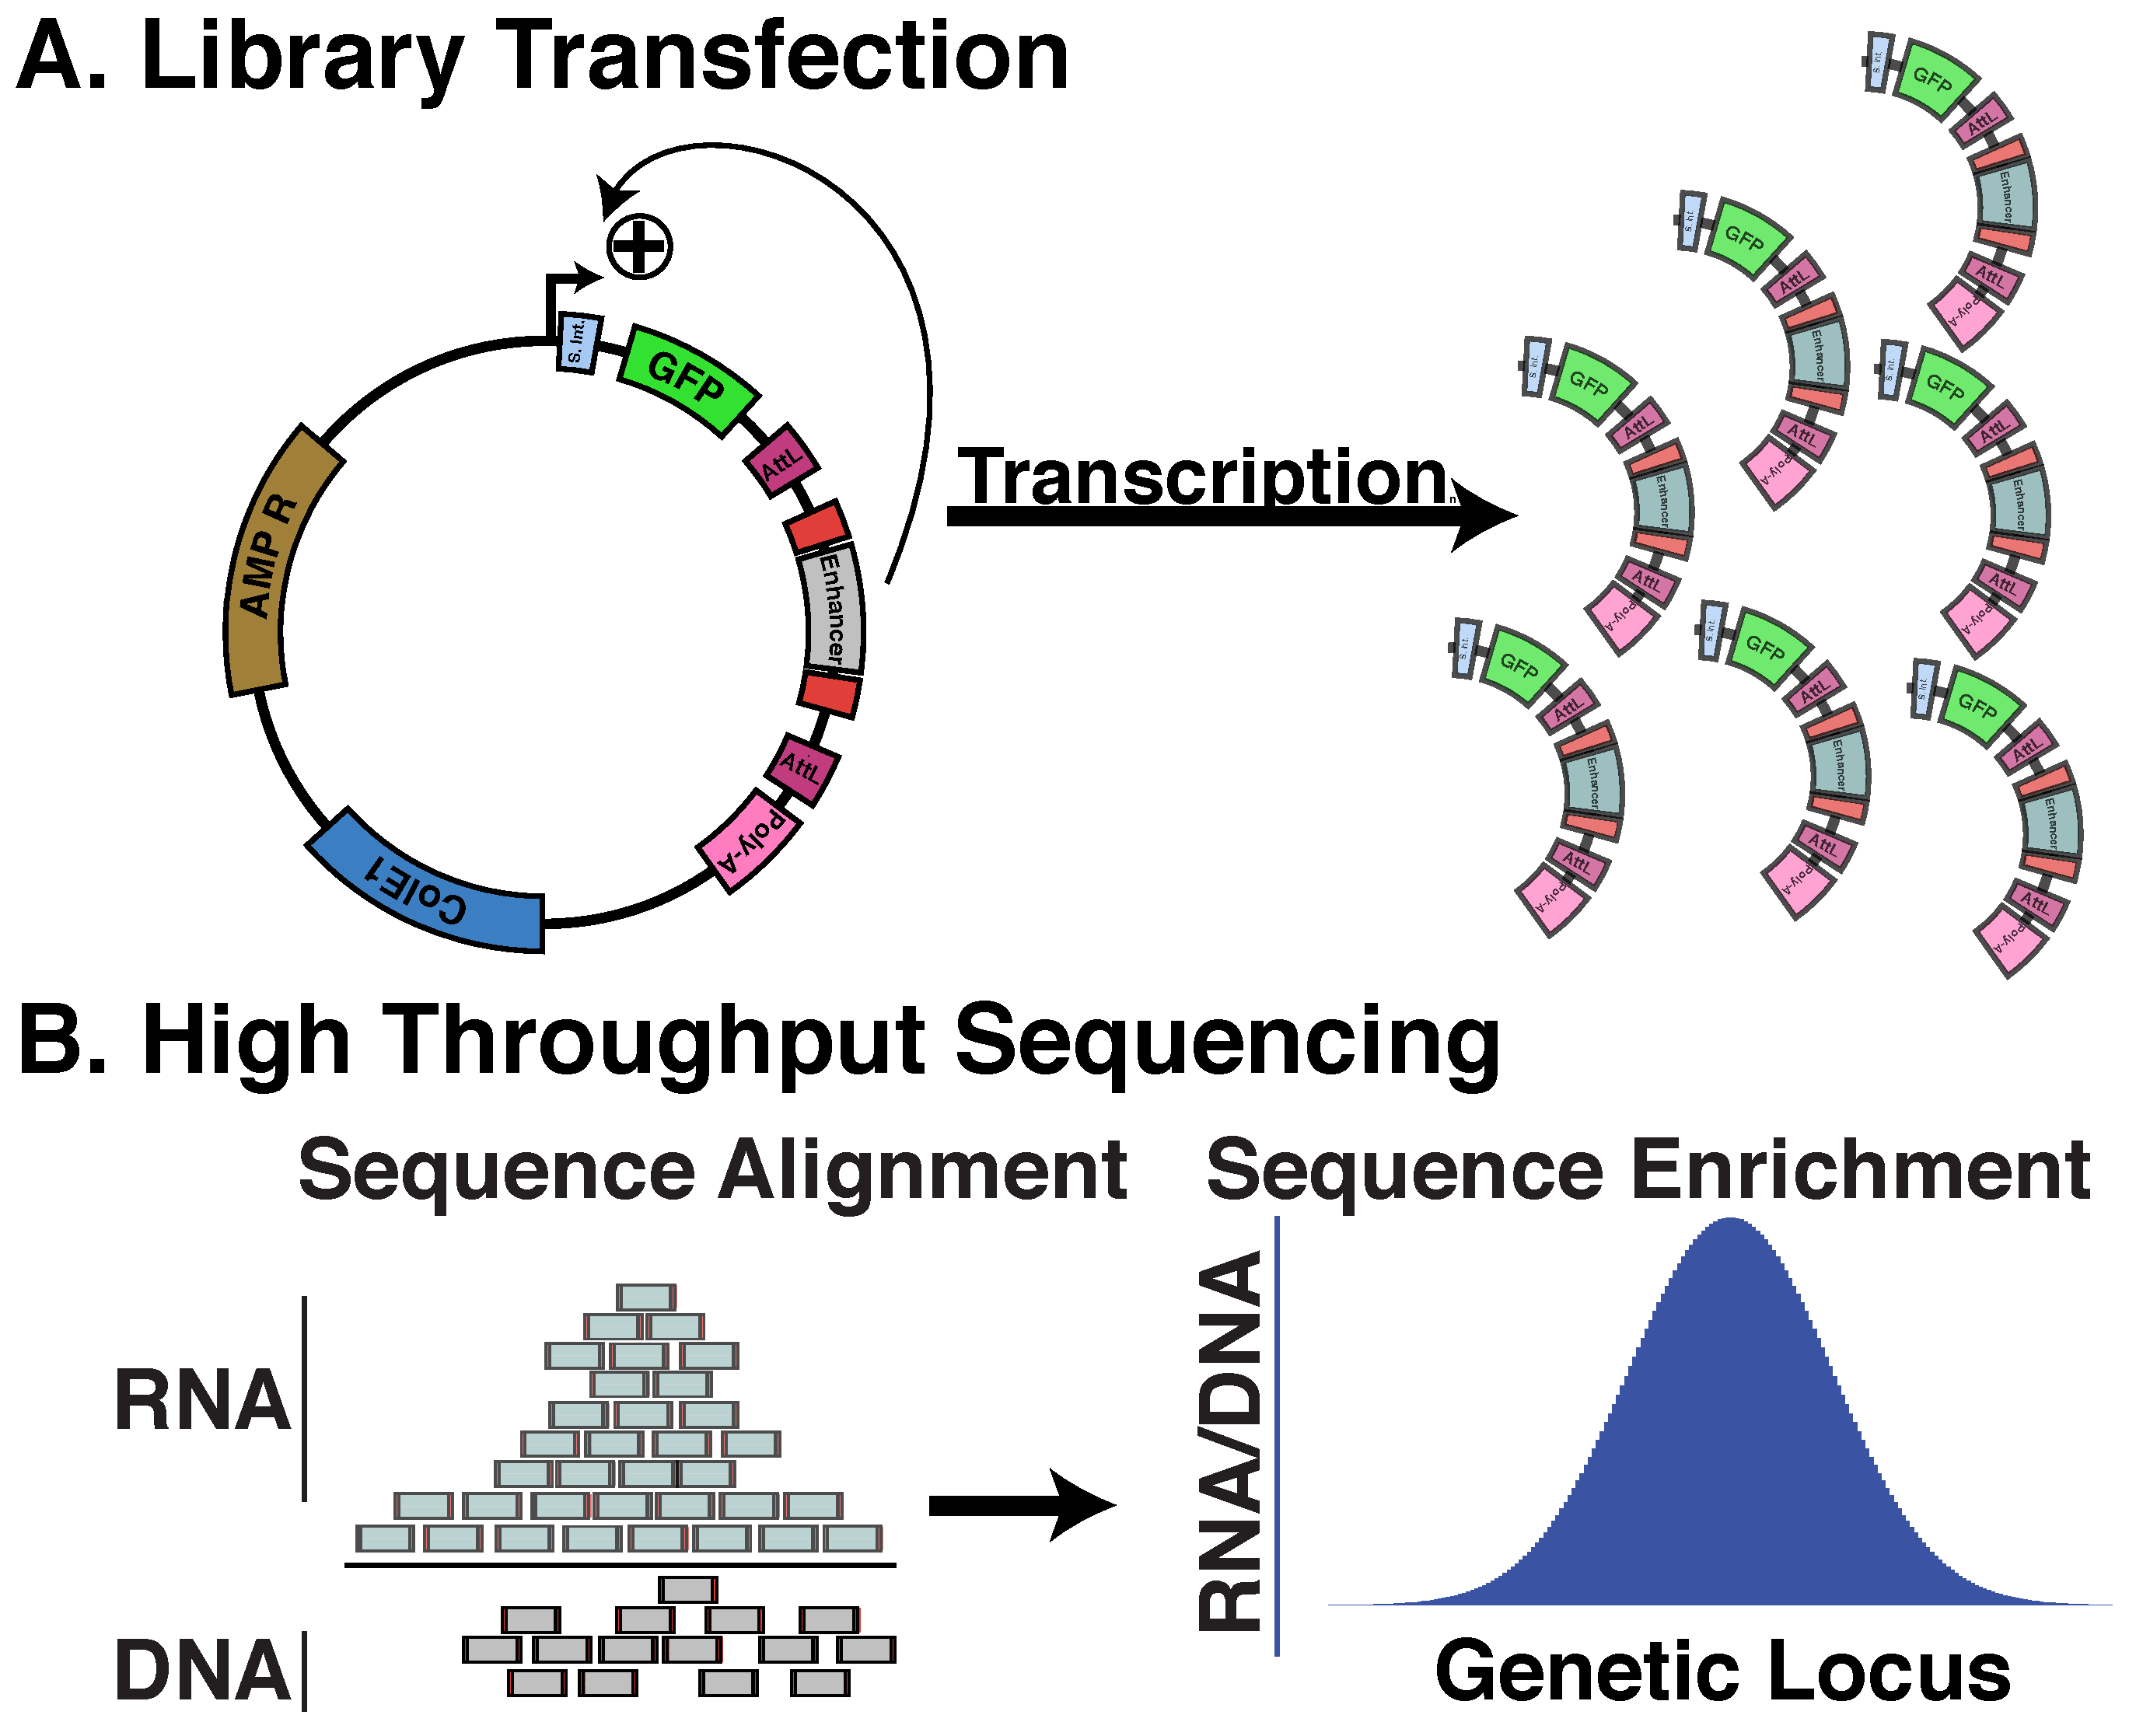
\includegraphics[width=1\linewidth, keepaspectratio=TRUE]{STARR_Fig/STARR_Mech.pdf}
		\end{center}
		\caption{\textbf{STARR-Seq Expression Mechanism}\label{fig:STARR_Mech}}		
        \textbf{A.} Once transfected into target cells library plasmids containing a fragment capable of driving transcription recruit the trans-factors to drive transcription from the nuclear trans-enviroment to the minimal promoter of the plasmid. The fragment is self-contained inside the transcript within the 3' UTR of the GFP Transcript. \textbf{B.} Once the transfected plasmid library and the mRNA transcript fraction are purified separately and sequenced via high-throughput sequencing, enhancers are identified through enrichment analysis of transcript molecules over input plasmid library molecules at a given genetic locus. 
	\end{figure}       
    \clearpage
}\normalsize    

\afterpage{
	\renewcommand{\arraystretch}{1.1}%
	\begin{table}[p]
		\begin{center}
			\scalebox{0.75}{
            \begin{tabular}{cccccccccc}

				Name	& 	Species	& 	Genome	& 	Chr	& 	Start	& 	End	& 	Human	& 	Chr	& 	Start	& 	End \\\hline

RP11-152E16	& 	Human	& 	Hg19	& 	3	& 	177085068	& 	177256575	& 	Hg19	& 	3	& 	177085068	& 	177256575\\
RP11-600O1	& 	Human	& 	Hg19	& 	11	& 	35014508	& 	35158907	& 	Hg19	& 	11	& 	35014508	& 	35158907\\
RP11-66E15	& 	Human	& 	Hg19	& 	4	& 	84035331	& 	84212030	& 	Hg19	& 	4	& 	84035331	& 	84212030\\
RP11-372G7	& 	Human	& 	Hg19	& 	11	& 	123975116	& 	124147918	& 	Hg19	& 	11	& 	123975116	& 	124147918\\
RP11-977N11	& 	Human	& 	Hg19	& 	20	& 	52261674	& 	52446501	& 	Hg19	& 	20	& 	52261674	& 	52446501\\
RP11-468O12	& 	Human	& 	Hg19	& 	16	& 	22884673	& 	23050195	& 	Hg19	& 	16	& 	22884673	& 	23050195\\
RP11-487K10	& 	Human	& 	Hg19	& 	14	& 	97736917	& 	97917241	& 	Hg19	& 	14	& 	97736917	& 	97917241\\

				\end{tabular}
                }
			\caption{\textbf{GM12878 BACs}}
			\label{GM12878 BACs}
		\end{center}
	\end{table}
	\clearpage
}\normalsize

%%STARR-Seq BAC Tiling
\afterpage{
	\begin{figure}[p]
		\begin{center}
			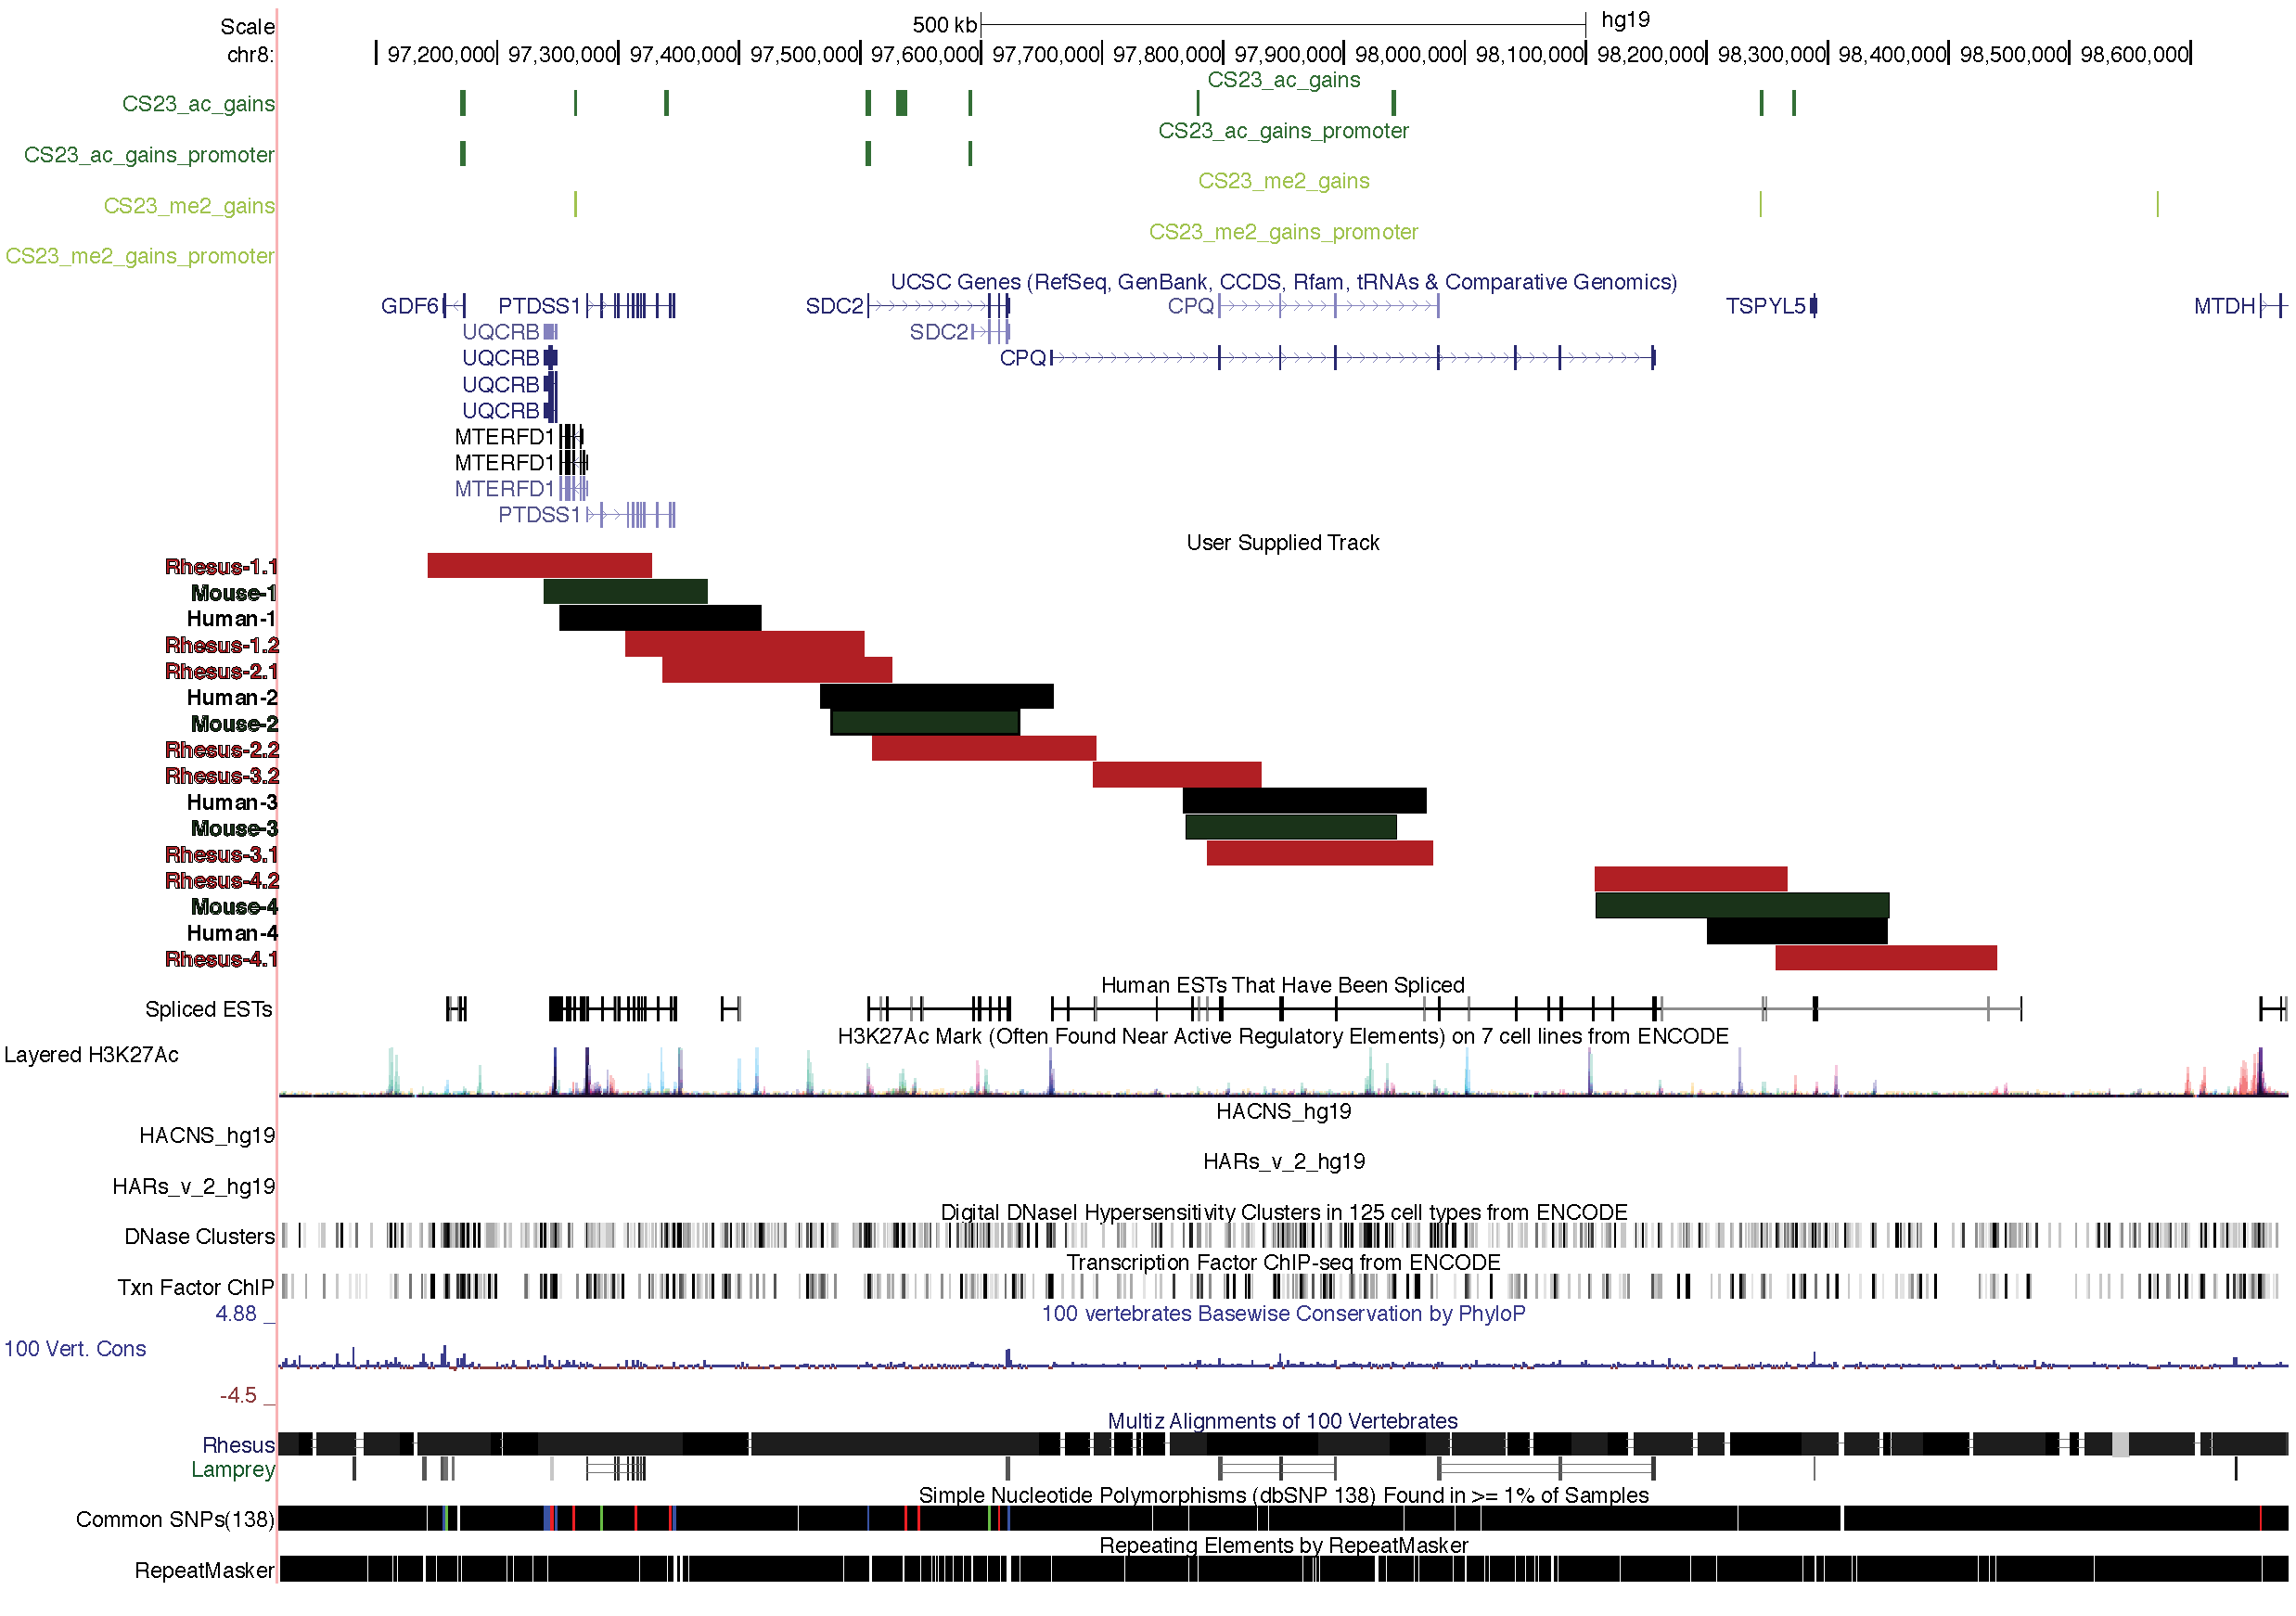
\includegraphics[width=1\linewidth, keepaspectratio=TRUE]{STARR_Fig/Syndecan_NC.pdf}
		\end{center}
		\caption{\textbf{STARR-Seq Bac Tiling}\label{fig:STARR_Tile}}		
         	This figure is a representative Neural Cluster containing the Syndecan2 gene, known to function in Wnt signaling pathways. Canidate human lineage gain of function promoters (light green) and enhancers (forest green) are represented above the gene (blue) track. BACs from Human (black) Rhesus (red) and mouse (dark green) are tiled across these gains or there orthologous locations to maximize coverage of every gain possible given the presence of orthologous sequence and BAC availability. 
	\end{figure}       
    \clearpage
}\normalsize 

%%Efficiency
\afterpage{
	\begin{figure}[p]
		\begin{center}
			\includegraphics[width=1\linewidth, keepaspectratio=TRUE]{STARR_Fig/Decay_FactorFig.png}
		\end{center}
		\caption{\textbf{2 Step Decay Model}\label{fig:STARR_Figure}}		
			With two efficiency steps, cloning and transformation. The library is much more susceptible to loose overall complexity than having a single step alone. 
	\end{figure}       
    \clearpage
}\normalsize

%%MPRA Mechanism
\afterpage{
	\begin{figure}[p]
		\begin{center}
			\includegraphics[width=1\linewidth, keepaspectratio=TRUE]{MPRA_Figures/MPRA_Basic_Fig.pdf}
		\end{center}
		\caption{\textbf{MPRA Expression Mechanism}\label{fig:MPRA_Mech}}		
			The MPRA assay relies on measuring candidate enhancers through their
transcriptional capacities in parallel. A Candidate Response Element is
cloned into a 5’ orientation to a MinP driven ORF with a 16 random base
pair tag between the ORF and Poly-A tail. Utilizing the proportion of
counts assigned to an individual transcript relative to that of the template
DNA activity is measured as a fold enrichment.
	\end{figure}       
    \clearpage
}\normalsize

%%MPRA Design
\afterpage{
	\begin{figure}[p]
		\begin{center}
			\includegraphics[width=.55\linewidth, keepaspectratio=TRUE]{MPRA_Figures/ExpOverview.pdf}
		\end{center}
		\caption{\textbf{MPRA Design}\label{fig:MPRA_Design}}		
			\begin{flushleft} \textbf{Top: }eVars were defined as: \textbf{1: }ancestral state is fixed across Chimpanzee, Orangutan, Macaque, and Marmoset. \textbf{2: }The derived human allele is fixed. For the purpose of interrogating human cortical development, eVars were filtered for overlap with candidate human-lineage gain of function developmental cortical enhancers.\textbf{Middle: }137bp fragments were centered on eVar coordinates from Human and Chimpanzee orthologs, multiple unique 16bp tags were added to each fragment. The fragment-tag library was cloned into the MPRA vector backbone with a Luciferase ORF and a minimal promoter between the fragment and tag. \textbf{Bottom: }The resulting plasmid library was transformed into hNSCs and tag expression was read out. Differential expression is called between discrete tag populations of orthologous fragments. \end{flushleft}.
        \end{figure}       
    \clearpage
}\normalsize

%%MPRA Fragments
\afterpage{
	\begin{figure}[p]
		\begin{center}
			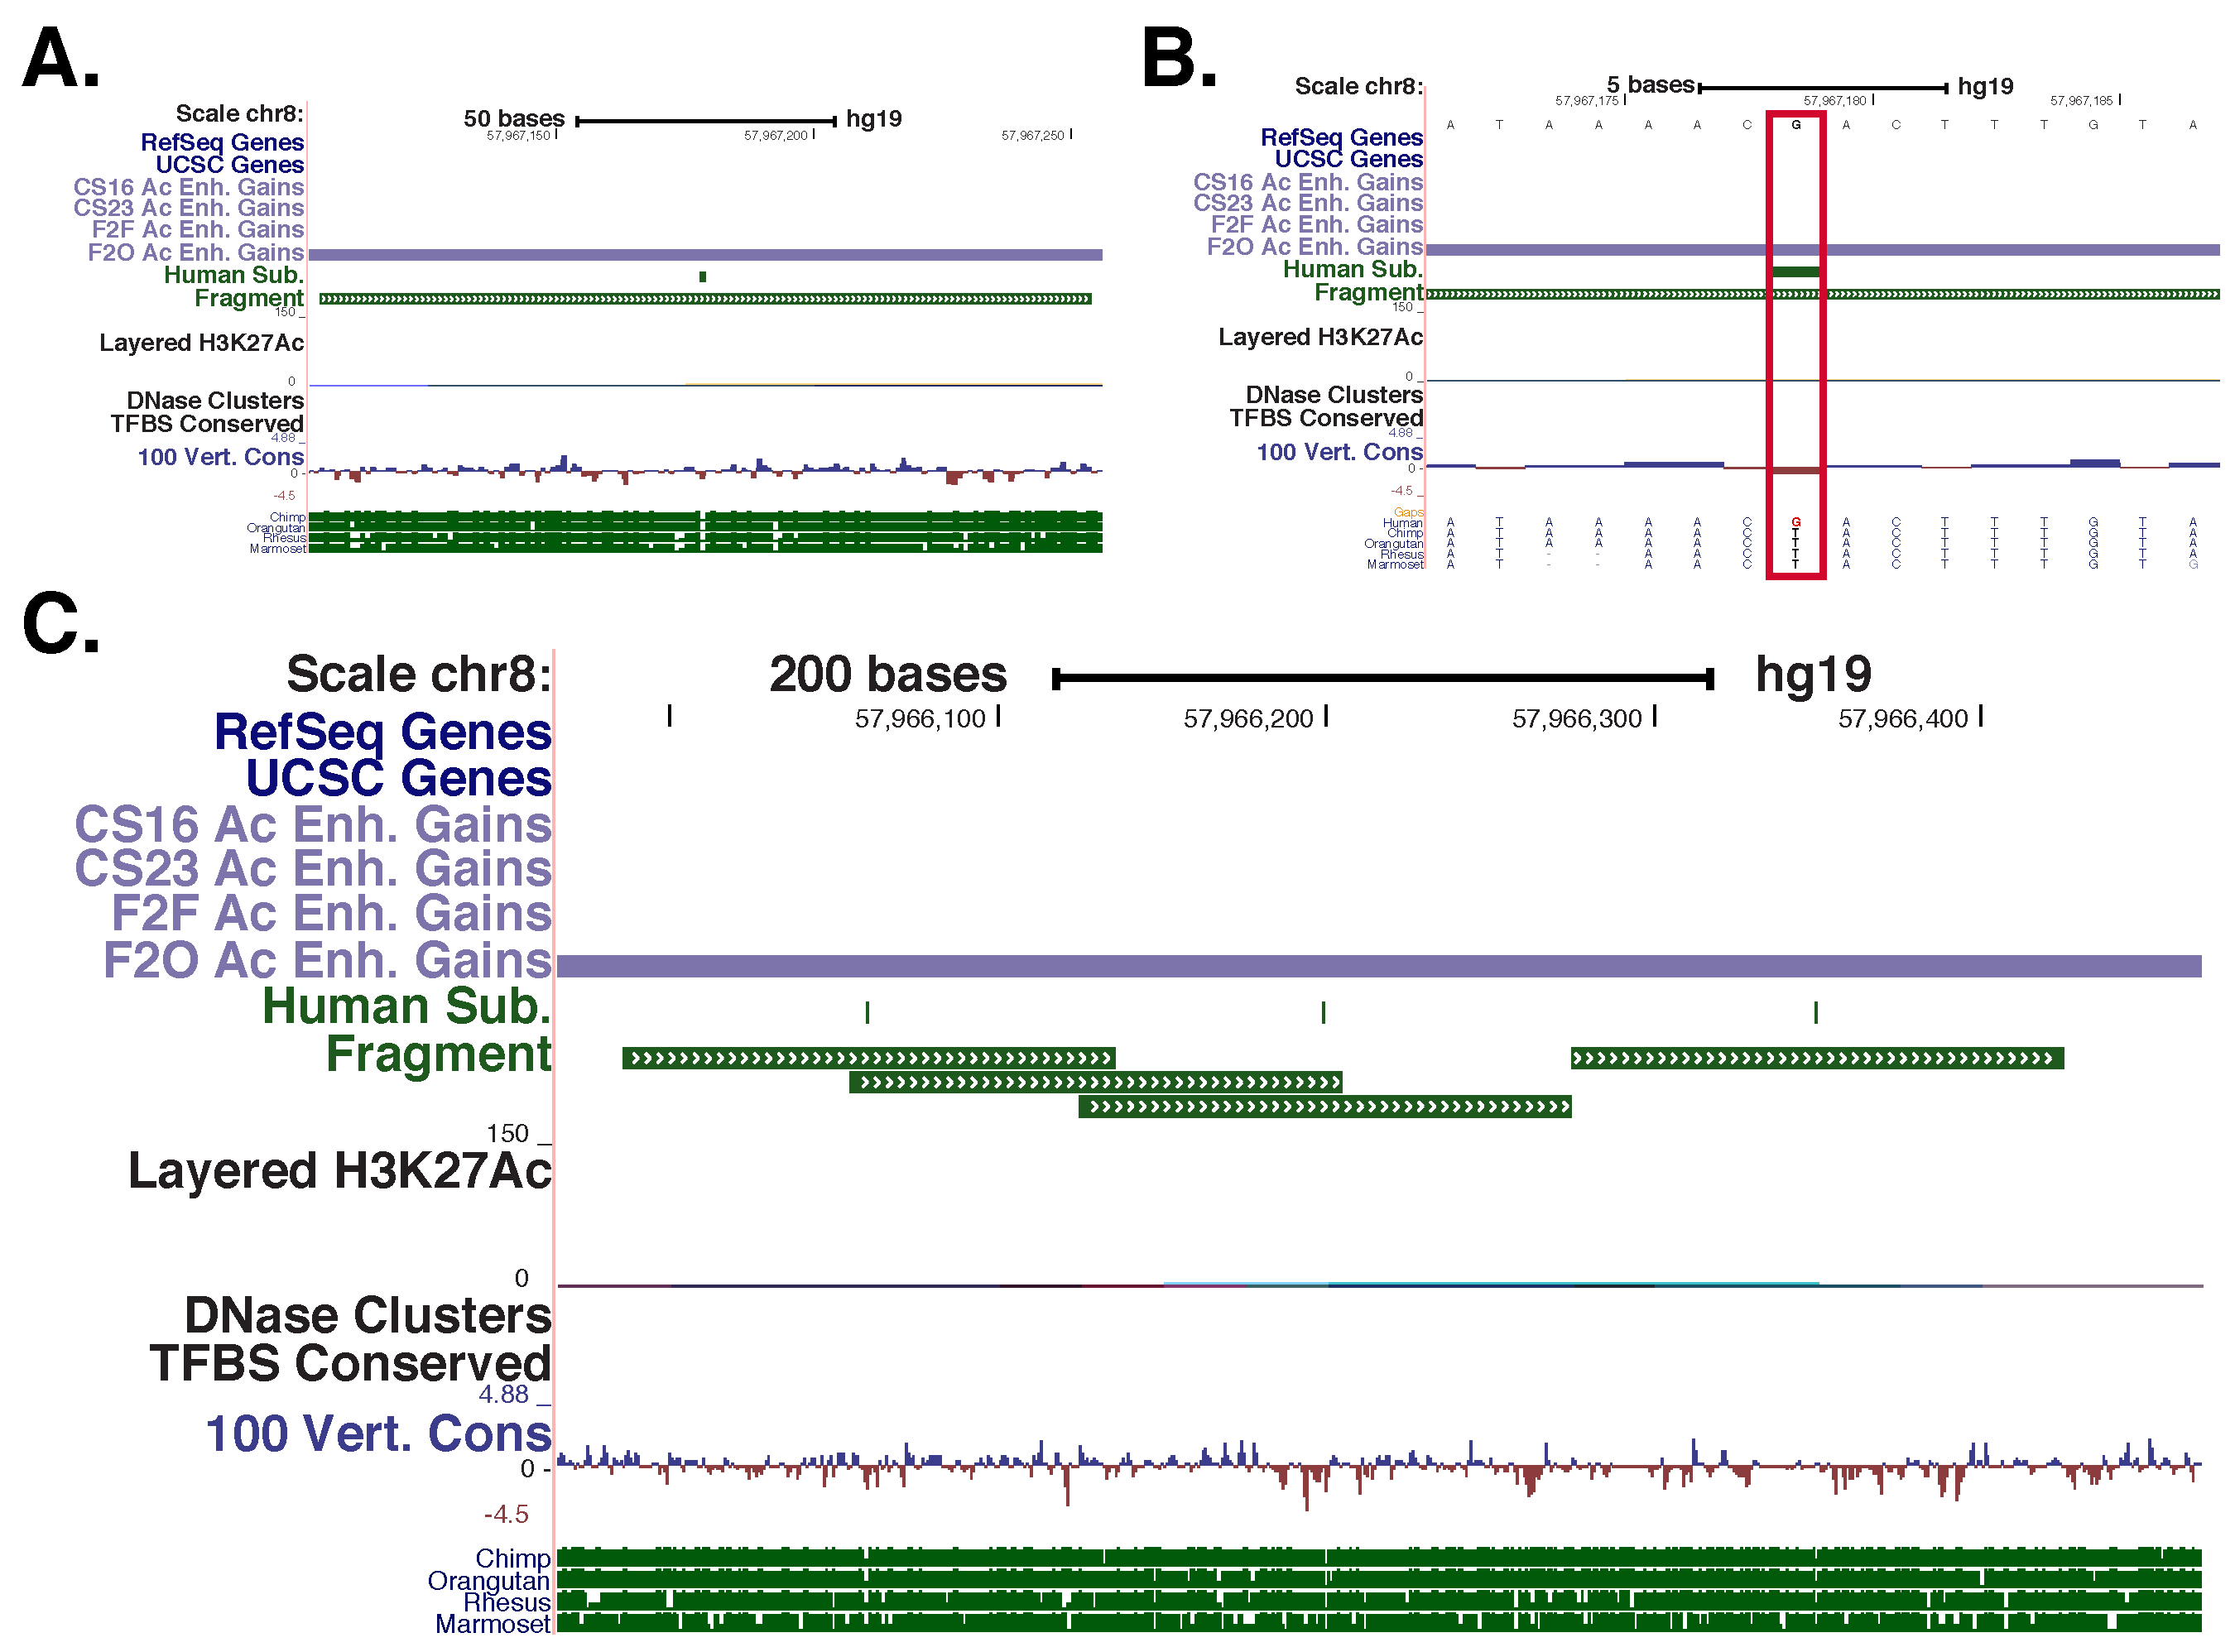
\includegraphics[width=1\linewidth, keepaspectratio=TRUE]{MPRA_Figures/MPRA_Fragments.pdf}
		\end{center}
		\caption{\textbf{MPRA Fragment Schema}\label{fig:MPRA_Frag}}		
			\textbf{A.} MPRA fragments of a length of 136-140bp were centered on called eVars within candidate human lineage gain of function developmental cortical enhancers, HANCS's, and HAR's. \textbf{B.} eVar bases were defined as base pairs within candidate human lineage gain of function developmental cortical enhancers, HANCS's, and HAR's which were conserved in the ancestral Chimp, Rhesus, Orangutan, and Marmoset alleles as well as being fixed in the derived human allele. \textbf{C.} When eVars fell within fragment range of each other an additional fragment was generated which centers the mid-point between fragments. When more than two eVars fell with fragment length, multiple additional fragments were generated pairwise across the set of eVars.
    \end{figure}       
    \clearpage
}\normalsize
\newpage
\section{Methods:}
	\subsection{STARR-Seq:}
    	\subsubsection{Library Construction:}
        	A detailed step by step methodology of the STARR-Seq protocol is provided in ppendix \ref{STARRMeathod}, this section will serve instead as a higher level overview. Input preparation was preformed on purified BAC or genomic DNA via sonication with a Misonix S-4000 sonicator at 20 amps, 47 watts for a total 1 minute in 1.5mL low adhesion eppendorf tubes. Tubes are submersed in cold circulating water, and runtime was split into ten second intervals interspersed with ten second delays between runtime. Every 2 intervals the tubes were removed and spun down. Sonicated genomic DNA served as input to NEBNext illumina library preparation (E6040L), size selected for an average fragment size of 500bp. Low cycle PCR amplification was preformed with tailed illumina primers which consisted of the attB gateway cloning arms. Gateway recombination reactions were preformed with 150ng of the gateway compatible STARR-Seq vector in a 2:1 insert to vector ratio at 25C overnight in a PCR machine. 4 reactions for BACs and 8 reactions per-genome were preformed. Library recombinations were pooled and cleaned up with 1x ratio of AMPureXP beads and eluted in 13uL of water per-four reactions. Recombined libraries were electroporated into MegaX DH10B Electro Competent cells(C6400-03), 2uL of recombination reaction was transformed per 20uL electrocompetent E.coli at 200 ohms, 25uFd, 2.0kV. Recovered reactions were pooled together and a dilution series was plated to assay total library complexity. The library was propogated in vivo in batches of 500mL terrific broth for every five transformation reactions. Once the culture OD reached 0.80 the library was pelleted for purification with the Qiagen EndoFree Maxi kit.
            
        \subsubsection{Library Transfection and Processing:}
        	GM12878 cells were transfected in two batches of 5 million cells each. Each batch consisted of 5 transfections of one million cells each with 1ug of purified STARR-Seq library. Cells were plated in 1.5mL of pre-warmed media and incubated for 24 hours. DNA and RNA were purified with the Qiagen DNA/RNA 2 in 1 All Prep kit (80204), with an on column DNAseI treatment to the RNA fraction. mRNA was isolated from total RNA with Dynabeads mRNA Purification Kit (61006) and cDNA first strand synthesis was preformed with Invitrogen SSIII (18080-400). Second strand cDNA synthesis was preformed with the NEB second strand synthesis module(E6111). The plasmid library was enriched from total genomic DNA with the Qiagen mini-prep columns (27106). Absolute copy number of recovered plasmid and transcript library was calculated via qPCR with a copy number standard of the STARR-Seq plasmid. Low scale PCR reactions were preformed with Illumina index primers (E7335L) and sequenced on Illumina Hi-Seq paired end 2x75bp. 
            
        \subsubsection{Read Down-sampling:}
        	Reads from \cite{Arnold:2013aa} were processed via alignment to the drosophila genome (dm3) with bowtie. Aligned reads from input and transcripts fractions were independently randomly shuffled using the unix shuffle command and the requisite percentage of total reads were taken from the header utilizing the head command in conjunction with the –n flag. These files were used as input to call peaks with a previously cited ChIP-Seq peak caller \cite{Reilly:2015aa} and a p-value of 0.0001.
        
        \subsubsection{Read Processing:}
        	Raw reads were aligned with bowtie using the flags bowtie -S -p 8 --chunkmbs 256 -m 1 -X 1500. BAC specific indexes were created from fasta files retrived from UCSC genome browser form the hg19, RheMac2, and mm9 genome builds. Reads were analyzed in a matrix of four options split by two conditions. The first condition was merging mate pairs into full read intervals to maximize coverage or just using the aligned 75bp reads alone. To merge mate pairs, aligned reads were sorted and converted to bed coordinates utilizing CGAT’s bam2bed.py publicly available script. The furthest combination of start and stop coordinates for each set of mate pairs was found and reported for every paired aligned read with a custom perl script. The second condition removed duplicated sets of coordinates through utilization of a custom written perl script. Peaks for these conditions were called using a previously cited ChIP-Seq caller at a p-value of 0.00001 \cite{Reilly:2015aa}. Common peaks were found with BedTools intersection liberally with any overlap and conservatively by only selecting overlapped regions. 
	Signal processing was preformed on sorted bed files of read coordinates. Bed files were converted into genome coverage bed files, then bigwig and finally to wig formats and normalized by read count per-million reads mapped. Normalized wiggle files were then converted back to bigWig format for visualization. 

    \subsection{MPRA:}
   		\subsubsection{Library Construction:}
        
	This section is a brief overview of the attached protocol developed for MPRA library construction (\ref{MPRA_Protocol}). The majority of Custom Array’s synthesized oligo products are truncated as a result of synthesis failure, in response a low cycle PCR is optimized with SYBR green to monitor amplification (See Section \ref{Prelim}) and preformed with common 15bp primers synthesized to on the 5’ and 3’ ends of every library olio (See Sections \ref{MPRAPrimer} \& \ref{Prime}). The degenerate 16bp oligo tag and requisite downstream cloning sites are added in a low scale emulsion PCR (ePCR) (See Section \ref{ePCR}). This reaction is seeded with the estimated multiplicity of transcript to micelle (MTM) of $\sim$0.2. This ratio ensures that no more than one molecule populates a single micelle, preventing unequal amplification and skewing of library representation beyond the bounds of synthesis constraints. It was debated weather or not this affected the single compartmental SYBR green PCR to enrich for full-length products, and ePCR would have been advisable for the initial amplification. Given results of Agilent High Sensitivity DNA Bioanalyzer traces of the initial library there was relatively undetectable amount of full length products to truncations, making the MTM of $\sim$0.2 unpractical to maintain library diversity. Alternatively size selection of an unknown amount of full length transcripts represented a risk not worth exploring, as percent loss and ability to detect the remaining fraction were uncertain. Given a lower valued sample these options would be worth exploring.
	
	Within the purified ePCR amplified fragment library there was size substructure, most likely as a result of primer slippage along a subpopulation of degenerate tags. To reduce any potential artificial bias of fragment representation as a product of tag composition the amplified fragments were size selected with a 2\% Agarose Pippen Prep Gel Cassettes (See Section \ref{Pippen}). As a general note this shoulder of sub products tends to arise after a threshold of amplification, therefore whenever amplifying the fragment library great care was take to identify the optimal cycle threshold to reduce these products from forming and also size exclude them moving forward. Fragment libraries and pMPRA1(Addgene) were digested separately with SfiI at 37$^{\circ}$C over night. pMPRA was treated with CIP at 37$^{\circ}$C for one hour. Fragment libraries were cleaned up with Qiagen MinElute columns while the plasmid backbone was isolated from the 600bp-excised insert by AMPureXP SPRI bead cleanup at a 1x volume ratio.
	
	Library ligation (See Section \ref{Lig}) into the MPRA vector backbone was preformed in multiple 20\textmu L reactions for the single species library and 40\textmu L reactions for the combined total fragment library. Reactions were seeded with a insert copy number to backbone molecular ratio of 3:1 and incubated in thin-wall PCR tubes in a thermocycler at 16$^{\circ}$C for 16 hours. In order to drive successful recombination each reaction received 2000U of fresh DNA Ligase. Recombination reactions were then pooled and cleaned with AMPureXP SPRI beads and concentrated into 10\textmu L. Purified inert library reactions were then electroporated into highly electrocompetent \textit{E.coli} (See Section \ref{Trans}). Most importantly in order to estimate total library complexity moving forward a dilution series of pooled and recovered transformation reactions was plated on LB-Amp plates and grown at 37$^{\circ}$C overnight. Multiple batches of 500mL LB-Amp liquid cultures were seeded with a range of pooled and recovered transformation reactions and grown at 37$^{\circ}$C and 225RPM until the OD was $\sim$0.95-1.2 (est. 8-11hr). Pellets were pelleted and stored at -20C. 

	The plating dilution series was used to estimate the overall library tag complexity in each pellet, and the library size was used to estimate the average tags per-fragment. For the combined human and chimp library I targeted an estimate of $\sim$80 Tags per-fragment. This figure was chosen as it should ensure a large enough tag count heighten the MPRA’s sensitivity, but low enough to yield reproducible tag count depth in a feasible number of sequencing reads. This step required several iterations of transformation and unfortunately the transformation efficiency is somewhat variable between transformation reactions regardless of using the same batch of reagents. If needed libraries were blended (See Section \ref{Blend}) from multiple pellets to achieve this complexity. This process was utilized after library purification, and blending was done in volumetric proportion to the estimated complexity of the source pellet to ensure equal proportionate representation of every fragment/tag combination across the final library with the bounds of stochastic variation by chance. Final Inert libraries were QC’s initially with multiple restriction digests to ensure the absence of self ligated backbone products or multiple insert recombinants (See Section \ref{fig:InertLib_Digest}), of note various minor ghost bands will appear on this analysis as individual degenerate tags will contain some of the shorter 6-8bp restriction sites. These bands are readily identifiable from undesired products due to their size and can be confirmed via a robust set of digests. Final library QC is preformed via 2x250bp sequencing (See Section \ref{InertLibSeq}), this stage is relevant to the previously discussed primer slippage on the 16bp tag sequence great care was taken to reduce and eliminate slippage product formation through throttling cycle number and size selection.
	
	The inert library and the MinP/Luc2 containing pMPRA donor plasmid (Addgene) were separately digested at 37$^{\circ}$C overnight (See Section \ref{CloneComp}). The Inert library was treated with CIP as previously discussed and the MinP/Luc2 containing ORF fragment was gel purified on a 0.8\% agarose gel. Alternatively to gel purification an additional digest with restriction enzymes specific to the backbone can be preformed until all backbone fragments are smaller than 1kB, then AMPureXP beads may be used to size select for the much larger ORF fragment. This strategy may improve overall yield for the user. Ligations were preformed with 500ng of linearized; CIP treated, and purified inert plasmid library and 650ng of purified MinP/Luc2 ORF for insert to backbone molecular ratio of 2:1. As before reactions were preformed in 20uL/rxn, in thin-walled PCR tubes at 16$^{\circ}$C for 16 hours in a thermocycler with 2000U of fresh DNA Ligase. Reactions were pooled and cleaned up with AMPureXP beads and concentrated by elution in 20\textmu L of Qiagen’s elution buffer. Purified competent library was transformed similar to before and complexity was estimated via plating a dilution series (See Section \ref{CompCalc}). Reactions were recovered and pooled and the entire recovered volume of transformed \text{E.coli} was grown in batches of 500mL LB-Amp for every 2 transformation reactions to a final OD of $\sim$1.9-2.0. Pellets were re-suspended, combined, and purified with Qiagen Endo-free Maxi plasmid prep kits. Quality control was ensured though high coverage representation of the inert library in the dilution series plating and restriction digest fingerprinting of the purified transfection grade competent library (See Section \ref{CompQC}). Tag representation was examined through 2x150bp sequencing of the competent libraries tag population (See Section \ref{BCSEQ}).

		\subsubsection{Library Transfection and Processing:}

        Competent MPRA libraries were transfected into 40 million hNSCs in batches of 4 million cells and 16\textmu g of plasmid library per-transfection utilizing an Amaxa Nucleofector under the electroporation program A-033 (See Section \ref{TransfectionConditions}). These conditions were chosen after preliminary optimization utilizing luciferase activity of the library as a whole to find the optimal conditions to maximize library signal (Figures \ref{fig:cell_Amt,fig:cell_Amt ,fig:cell_Amt}). Transfected hNSCs were recovered in pre-warmed media, pooled, and plated in two T-150 vented flasks. Cells were allowed to grow and recover for 6 hours. This amazingly inconvenient incubation time was chosen after a luciferase time series as well as a more specific time series which included RNA recovery, cDNA synthesis and, qPCR comparison of the Luciferase transcript levels indicated 6 hours as the optimal time point for maximum library expression before transcript attenuation (Data not shown). This time frame falls within the range suggested by Amaxa nucleofection with Luciferase ORFs accounting for the lag of transcript production to Luciferase signal. 

	Cells were harvest and pooled. Genomic DNA was purified from $\sim$5\% of the total cell harvest, while RNA was purified from the remaining 95\%  (See Section \ref{PostProcess}). Total RNA was subjected to a second aqueous DNAseI treatment, integrity was confirmed via Agilent Eukaryotic Pico Chip analysis, and mRNA was not isolated from total RNA to prevent any possible loss of MPRA transcript. Plasmid library was enriched from whole genomic DNA utilize Qiagens plasmid mini prep column and ERC buffer. cDNA synthesis was set up to drive transcript production efficiency as high as possible. Reactions were scaled to 2.5x the size and Input total RNA was restricted to 3.5-4\textmu g. Additionally, synthesis reactions were preformed at 50$^{\circ}$C for 2.5hr in a thermocycler with the lid temperature set to 55C. Reactions were pooled, purified and concentrated minelute columns. 

	Transcript and plasmid template was estimated in the cDNA and pDNA fractions, respectively, via qPCR off the Luciferase template (See Section\ref{MPRAqPCR}). Absolute copy number quantification was required and for this purpose careful serial dilution of the competent, untransfected plasmid library served as a comparison. The pDonor plasmid is a possible substitute, but it’s not recommended to use non-library sources of Luciferase as these templates may contain small mutations, potentially affecting primer annealing. The most useful range was a tenfold dilution range of 100 million to 100 copies of the competent library plasmid. Sample in put were 10 and 100-fold dilutions of the recovered enriched pDNA and purified cDNA fractions. PCR amplification of tag libraries by fraction are seeded at a constant 20 million copies per-reaction (See Section \ref{LastAmp}). Reactions were cleaned up and concentrated with a 1x volume ratio of SPRI beads, which are vital in this step as they functional as a size exclusion method to reduce high molecular weight transcripts from occluding analysis of the smaller molecular weight tag containing PCR amplicons. Once more amplification cycle number of 14 was determined via SYBR green observation and secondary product formation was observed via analysis with Agilent High Sensitivity DNA Chips. 

		\subsubsection{Read Processing:}
        
	Raw inert library fastq reads were processed according to Figure \ref{fig:MPRA_Data} with the data processing pipeline in inert mode (Script \ref{Code:Pipeline}). Inert reads were trimmed with fastx trimmer to remove the degenerated base pairs added to the tails of the amplification primers (See Section \ref{MPRAPrimer}). The degenerate base pairs increase 5’ heterogeneity of the transcripts and requires less PhiX DNA to be doped into the sample for illumina high-throughput sequencing resulting in higher clustering and a greater amount of total useable reads per-lane. Although these base pairs tend to be lower in quality as they are at the first base calls, removal of these bases facilitates down-stream analysis, which utilize on base quality.
	
Reads were then stranded, a process that rearranges the randomly annealed mate pairs into the same orientation, where mate pair one is the 5’ to 3’ fragment which begins upstream of the CRE, and mate pair two is the 5’ to 3’ fragment beginning downstream of the tag sequence. This ensures that when mate pairs are assembled together every contig will correspond to the same template strand, facilitating trimming assemblies into CRE and tag sequences. Mate pairs are assembled with pear and a base quality threshold of –Q 33 is enforced which trims all sequence downstream of the first consecutive bases below a Phred quality score of 33. Sequences are trimmed with cutadapt to first remove the 5’ and 3’ vector template. Finally the interstitial vector template is used as the 5’ adaptor sequence to trim for tag sequences and as a 3’ sequence to trim for CRE sequences. 

CREs sequences were then aligned to the library bowtie2 index sequence. The bowtie2 index was created by taking the merged bed coordinates of all fragments by species, padding them by 10 base pairs, retrieving the sequence fasta data in batch from UCSC genome browser for the corresponding species (hg19 for human fragments and panTro2 for Chimpanzee sequences), and creating libraray index with the bowtie2’s bowtie2-build function. To QC this library reference all library fragments were aligned to the index and checked for uniquely mapping100 percent sequence matches. Finally a translation file was created utilizing the library contig, start position, end position, and length of each library element’s alignment delimited by underscores in order to translate the CRE alignments form the inert data set. Fragments were aligned utilizing bowtie2’s ‘--end-to-end’ mode functionally making bowtie2 a global alignment method. The global alignment, custom index, and stringent alignment restrictions in the translation file were necessary as overlapping CREs in regions of clustered eVars were highly similar and reads were mistakenly multiply mapped to library elements with equal alignment scores and therefore alignments were chosen at random from the tied highest alignment scores. While this phenomenon does no necessarily affect other technologies, as the alignments are in virtually the same region, in the MPRA this results in a single tag being falsely assigned to two CRE elements and therefore it would be restricted from analysis. 

	After alignment, aligned CRE sequences are parsed to substitute the alignments and identify the aligned fragment utilizing the previously discussed translation file. Alignment statistics of matches, mismatches, insertions, deletions, and clipping are extracted as well. These are used in an R sub-module (See Script \ref{Code:ProcessRPipeline}) to create a percent identity score. We define percent identity as the percent of bases in the total alignment matching the reference. This is used with the user inputted percent identity threshold, for the purpose of our analysis we used a 98 percent ID threshold ensuring that no CRE in the analysis had more than 2 mismatches, insertions, or deletions. These CRE’s were then annotated with their corresponding tag sequences. Annotated tag sequences associated with multiple CREs and which were less than or greater than 16bp were filtered out of the final dataset and a final counts file of tag-CRE associations was tabulated. 

	Competent, experimental cDNA and, experimental pDNA fastq reads were processed the in the same manner with the corresponding competent and experimental run modes of the data processing pipeline (Script \ref{Code:Pipeline}). Process steps are conceptually the same as inert mode through mate-pair alignment contig assembly with pear, after which tag trimming the plasmid backbone with cutadapt directly isolated sequences. The resulting tag sequences were filtered for tags of only 16bp and counts were tabulated. Cross representation of tags along with their counts in the inert and competent library mode can be isolated with the data process pipeline’s tag comparison run mode. Finally, the counts of all sequencing runs can be aggregated into a single file for data analysis by running the data processing pipeline in annotation mode. 

		\subsubsection{MPRA Data Analysis:}

The entire annotated counts file was imported into and processed in R (Figure \ref{fig:MPRA_Data} and Code \ref{ Code:ProcessRPipeline}). Tags present in the competent library and experimental library were defined as tags, which had count values in either replicate of both, cell lineages. Counts were normalized to counts per-million reads (CPM) for transcript and plasmid counts for each replicate. Average plasmid tag CPM Average CPM for lineages was calculated for transcript and plasmid fractions. CPM values were Log2 transformed into a normal distribution. The density distribution of total average Log2 transformed plasmid fraction values across all replicates was used to empirically define and exclude tags based on low coverage driving stochastic deviation from population based replication across experimental replicates. Tag based activity was calculated as fold change transcript versus plasmid signal for lineage average values $(log2(Transcript_CPM) - log2(Plasmid_CPM))$. Tag activities were quantile normalized and fragment activity values for visualization were assigned as median tag activity value for each fragment. Fragments were filtered based the number of descriptive tags as defined by the correlation of median activity values between down-sampled tag activities for each fragment. Down-sampling was done via calling a python down-sampling script and an R sub-module to process sampled tags \ref{Code:DownSample}. Fragment activity p-values were calculated with a Wilcoxon Rank-Sum Test between each individual fragment’s tag activity distribution and the distribution of all other tag activities for each lineage replicate independently. P-values were Bonferroni corrected and fragments with a significant p-value at an FDR of 10\% within each independent replicate were defines as active (Code \ref{Code:Index} and \ref{Code:Activity}). For orthologous allelic eVar fragments, which were still paired after tag and fragment quality control, differential allelic activity p-values were calculated with a two-tailed Wilcoxon Rank-Sum Test between the tag activity distributions of both alleles. P-values were Bonferroni corrected and allelic pairs with significant p-values below at an FDR of 10\% within each independent replicate were defines as differentially active(Code \ref{Code:DiffActivity}). 

		\subsubsection{Barcode Down-sampling:}
        
In the primary analysis (Script \ref{Code:MPRA_Analysis}), all fragments with tag counts of 20, 40, 60, 80, and 100 were selected the final tag list into independent files. The tags were down-sampled (Script \ref{Code:Rand}) 1 to half the amount of tags, tags were randomly selected without replacement into two files. An R sub-module (Script \ref{Code:QMod}) was called which loaded each random permutation file, assigned the median tag activity of permuted tags to the corresponding fragment and quantile normalized the population of median activities by fragment. Finally the two randomly selected median activity populations were correlated via the Pearson Correlation. This resulted in Pearson Correlations between synthetic tags replicates as a function of increasing tag count to empirically measure a lower-bound cut-off of tags by fragment. 

%%STARR-Seq Lib Construction
\afterpage{
	\begin{figure}[p]
		\begin{center}
			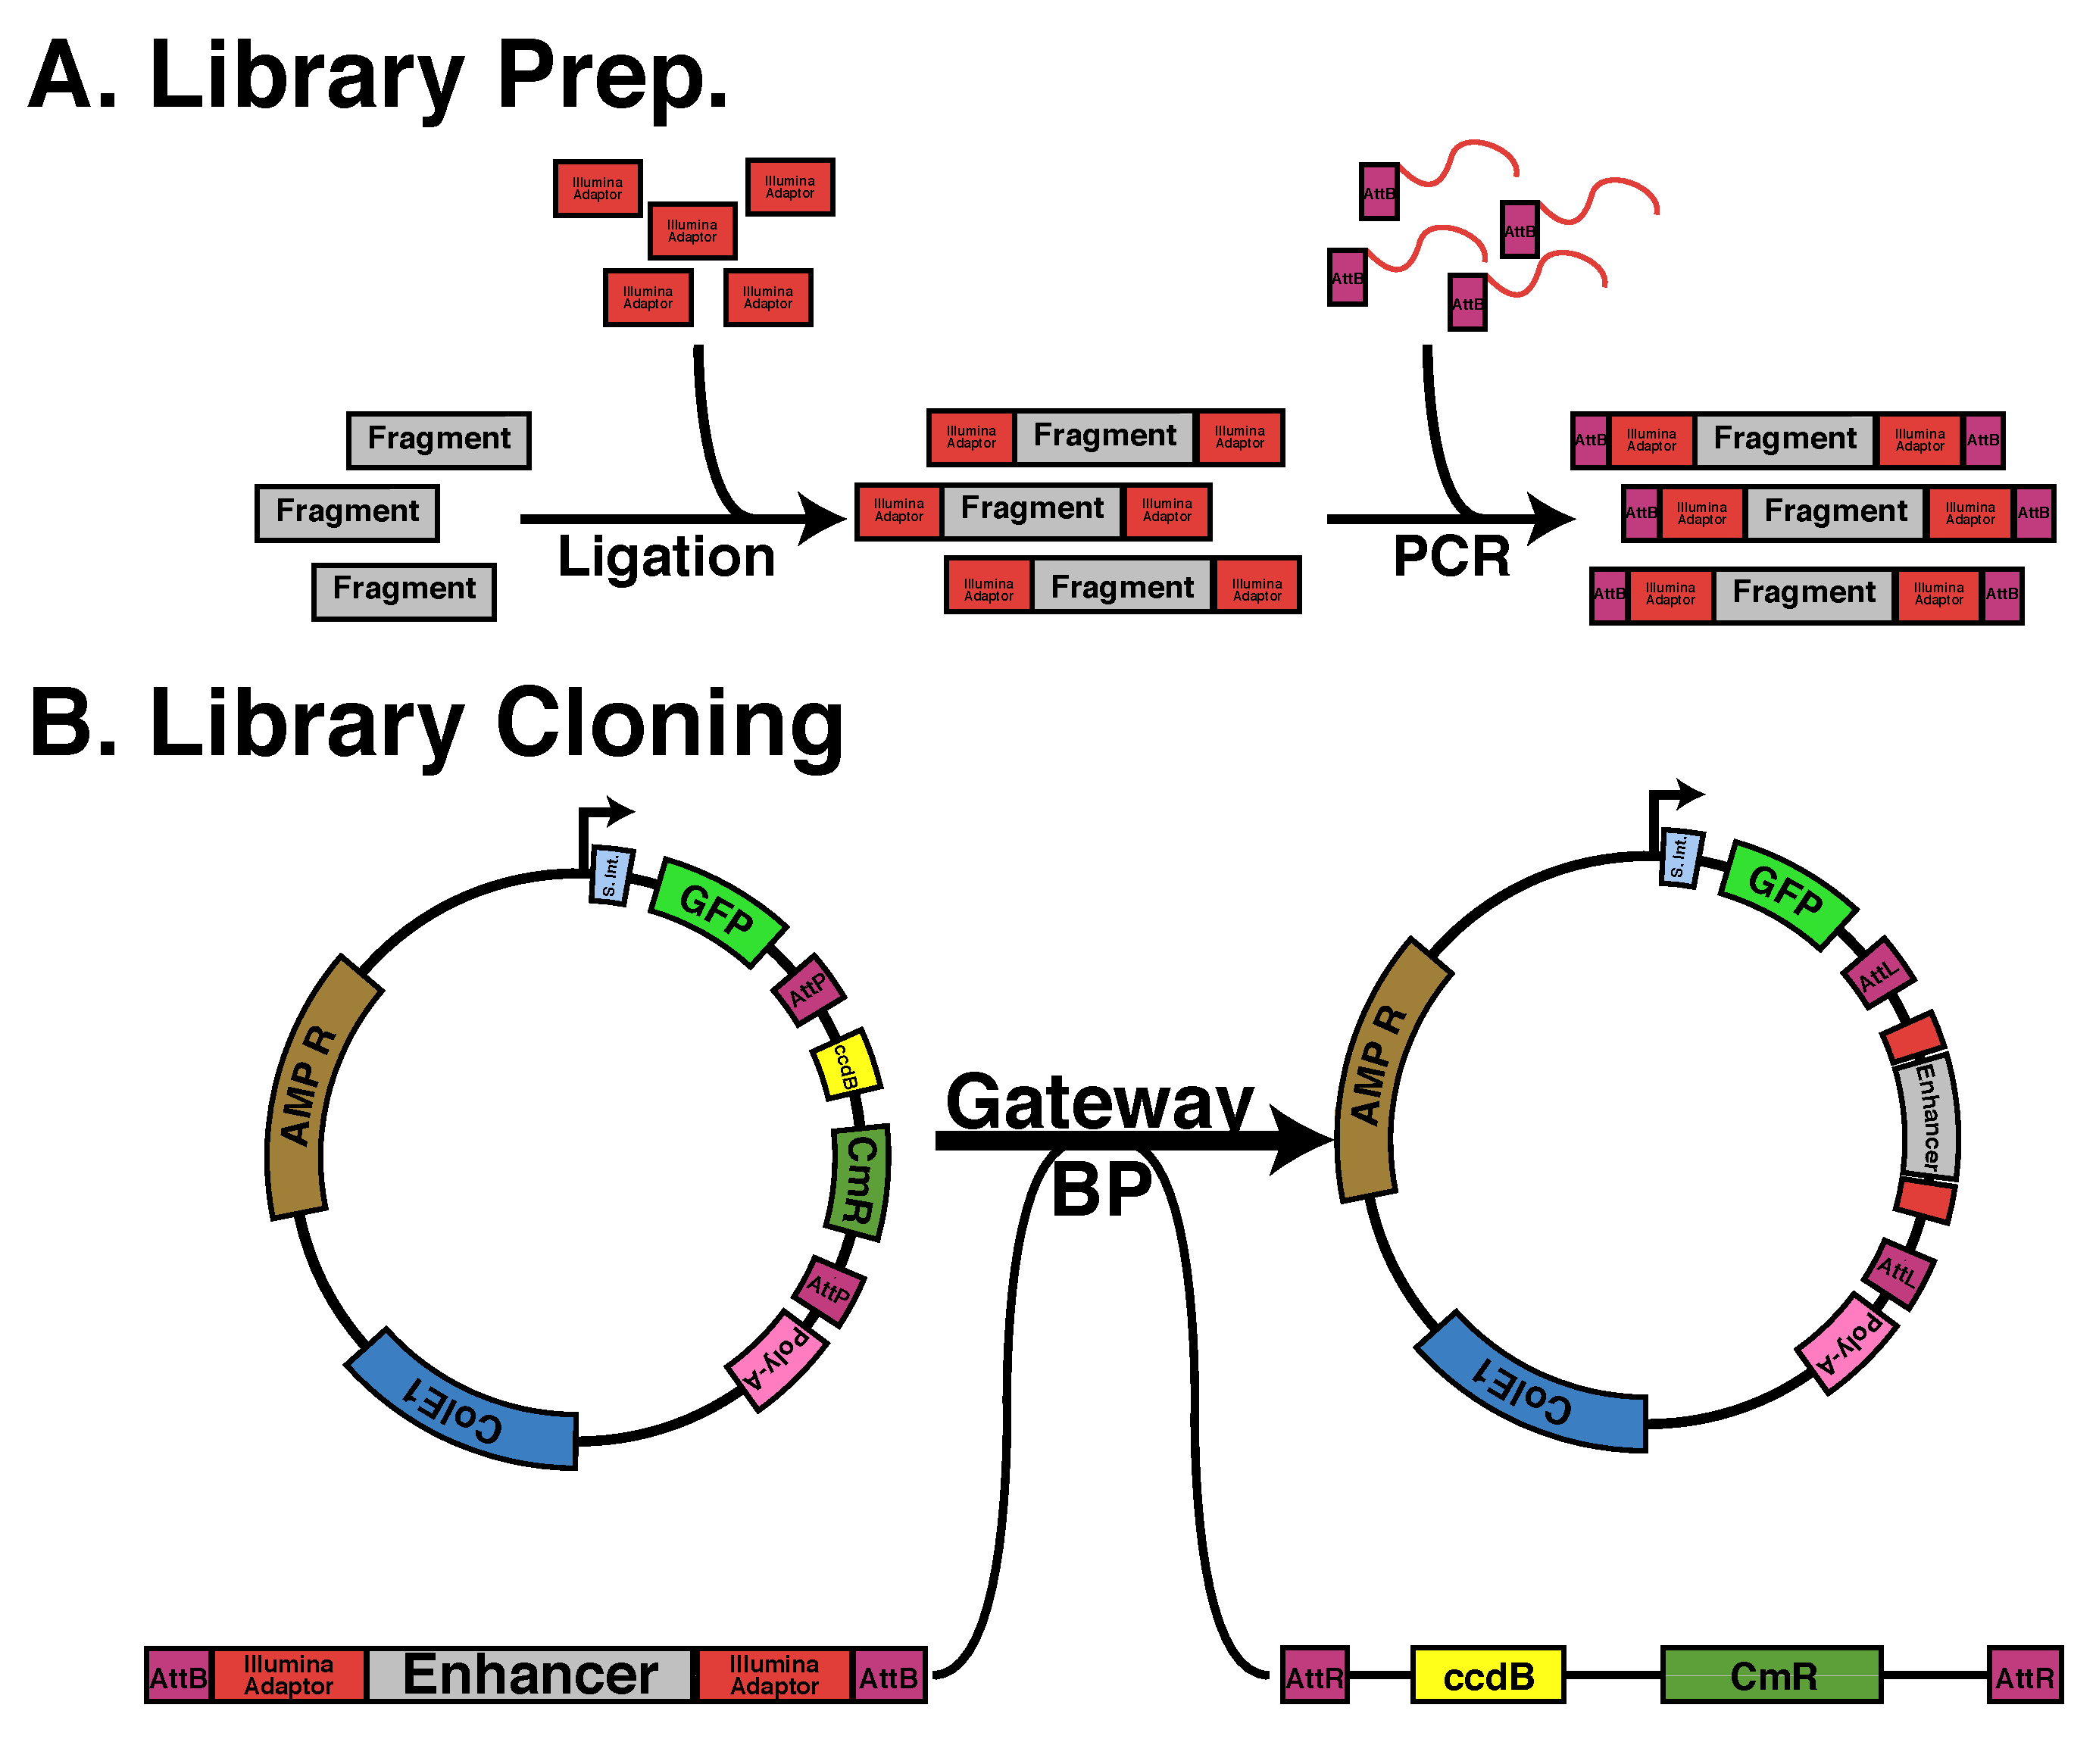
\includegraphics[width=.95\linewidth, keepaspectratio=TRUE]{STARR_Fig/STARR_Cons.pdf}
		\end{center}
		\caption{\textbf{STARR-Seq Library Construction}\label{fig:STARR_Cons}}		
        	\textbf{A.} Input genetic material is sonicated into smaller 200bp-1Kb fragments. Sonicated fragments are then end repaired, dA tailed, and ligated to illumina high-throughput sequencing adapters with the NEBNext Illumina high-throughput library prep kit (E6040L). After size selection with AMPureXP beads for the target fragment size AttB Gateway homology arms are added through a low-cycle PCR amplification. This helps add redundancy to the library while also maintaining overall library complexity. \textbf{B.} The library fragments are then cloned into the STdONR vector, which is the STARR-Seq vector with the p-DONR fragment in place of the original cloning site through the gateway BP reaction. Recombination reactions are the cleaned up and transformed in multiple batches into highly electrocompetent \textit{E.coli}. Non-recombined vectors are eliminated via the ccDb suicide gene contained within the p-DONR fragment allowing propagation of the recombined library fragments. Propagation is stopped at an OD of 0.8-1.0 and the library is purified for transfection. 
	\end{figure}       
    \clearpage
}\normalsize    
    
%%MPRA Lib Construction
\afterpage{
	\begin{figure}[p]
		\begin{center}
			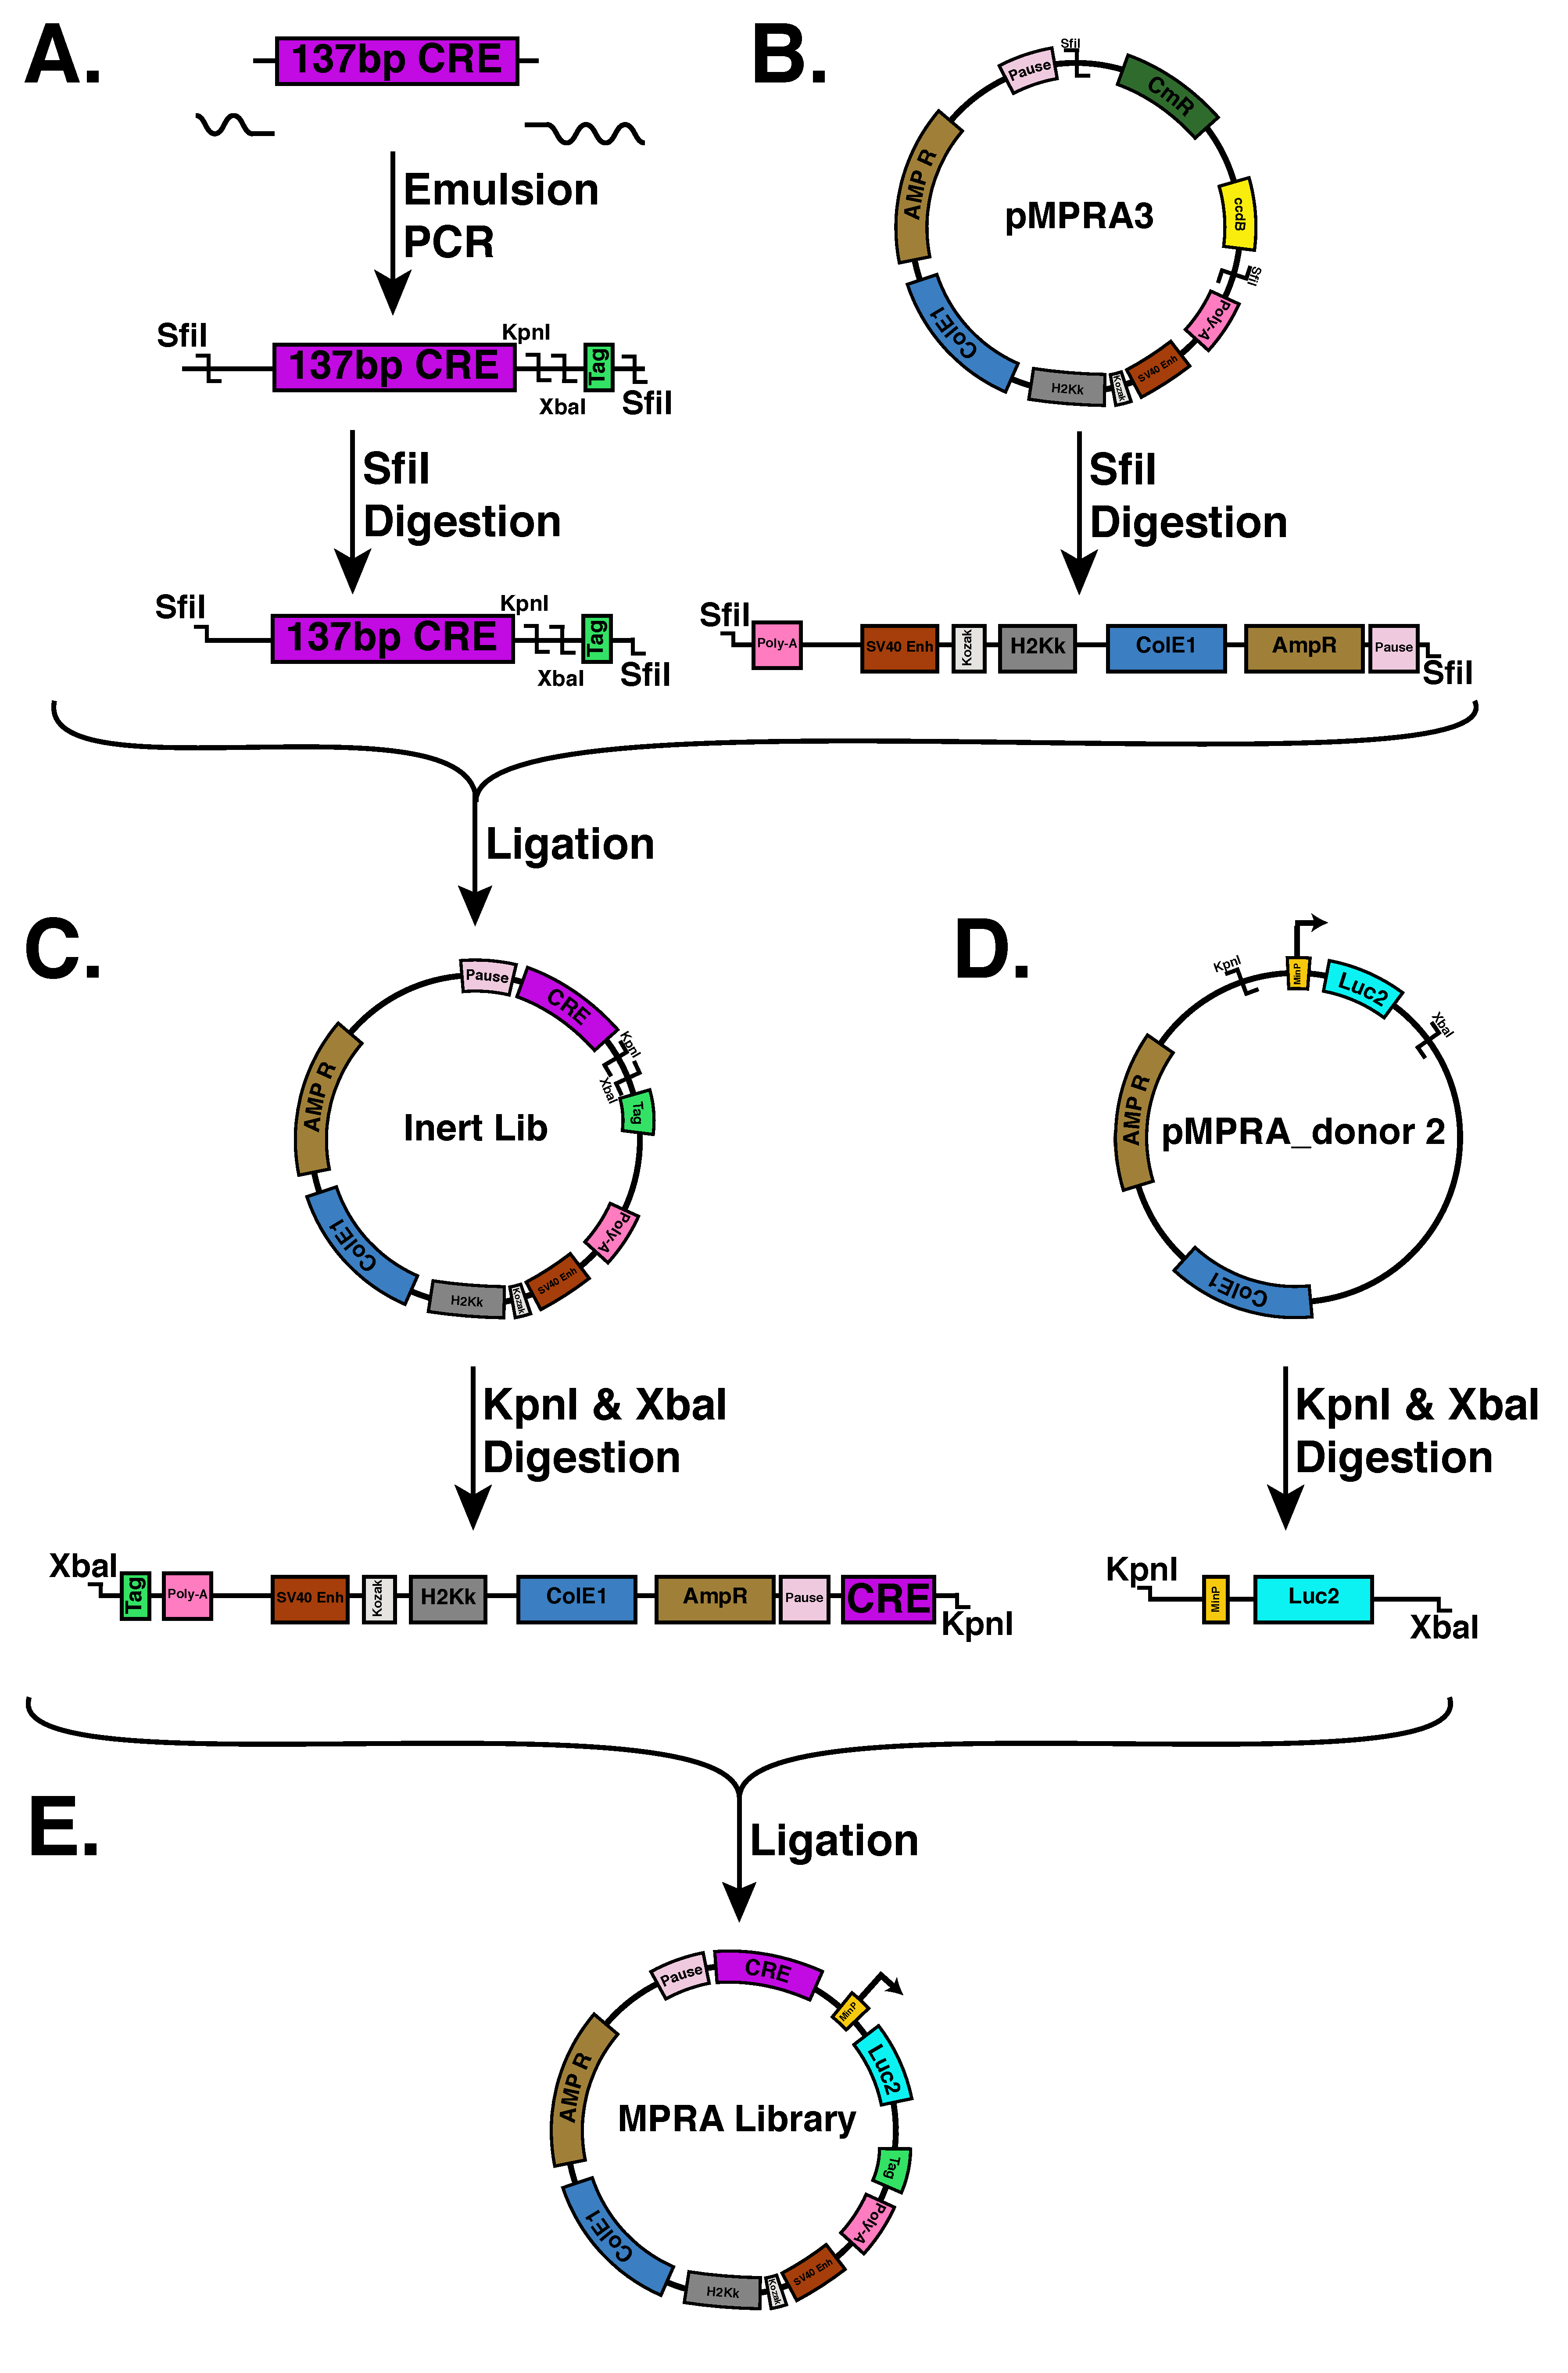
\includegraphics[width=.66\linewidth, keepaspectratio=TRUE]{MPRA_Figures/MPRA_LibConstruction.pdf}
		\end{center}
		\caption{\textbf{MPRA Library Construction}\label{fig:MPRA_Cons}}
			\textbf{A.} After low scale amplification under SYBR Green observation and size selection to enrich for full length, successfully synthesized library oligos are amplified in a lowscale emulsion PCR. Primer over hangs add 3' and 5' Sfi restriction sites to clone the library into the MPRA plasmid, the 3' 16bp degenerate oligo tag, and the 3' KpnI and XbaI restriction sites for ORF cloning. The Fragment library is then digested with SfiI over night and purified. \textbf{B.} MPRA vector is linearized via SfiI digestion over night, treated with CIP, and purified. Digested library and vector are ligated overnight at room temperature, transformed into \textit{E.coli} in multiple batches and grown to an OD of 0.8-1.0. The resulting purified inert library can be characterized and tag assignments can be made via 2x250bp sequencing. \textbf{C.} Inert library is linearized via digestion with KpnI and XbaI overnight at room temperature and treated with CIP. \text{D.} The MinP/Luc2 ORF is cut out of the pMPRA Donor plasmid via digestion with KpnI and XbaI over night at room temperature. \textbf{E.} Purified and linearized plasmid library is then ligated to purified and linearized MinP/Luc2 ORF to form the competent library. The resulting competent library is transformed into highly electrocompetent \textit{E.coli} and grown in batch to a final OD of $\sim$2.0.
	\end{figure}       
    \clearpage
}\normalsize

%%MPRA Data Processing and analysis pipeline
\afterpage{
	\begin{figure}[p]
		\begin{center}
			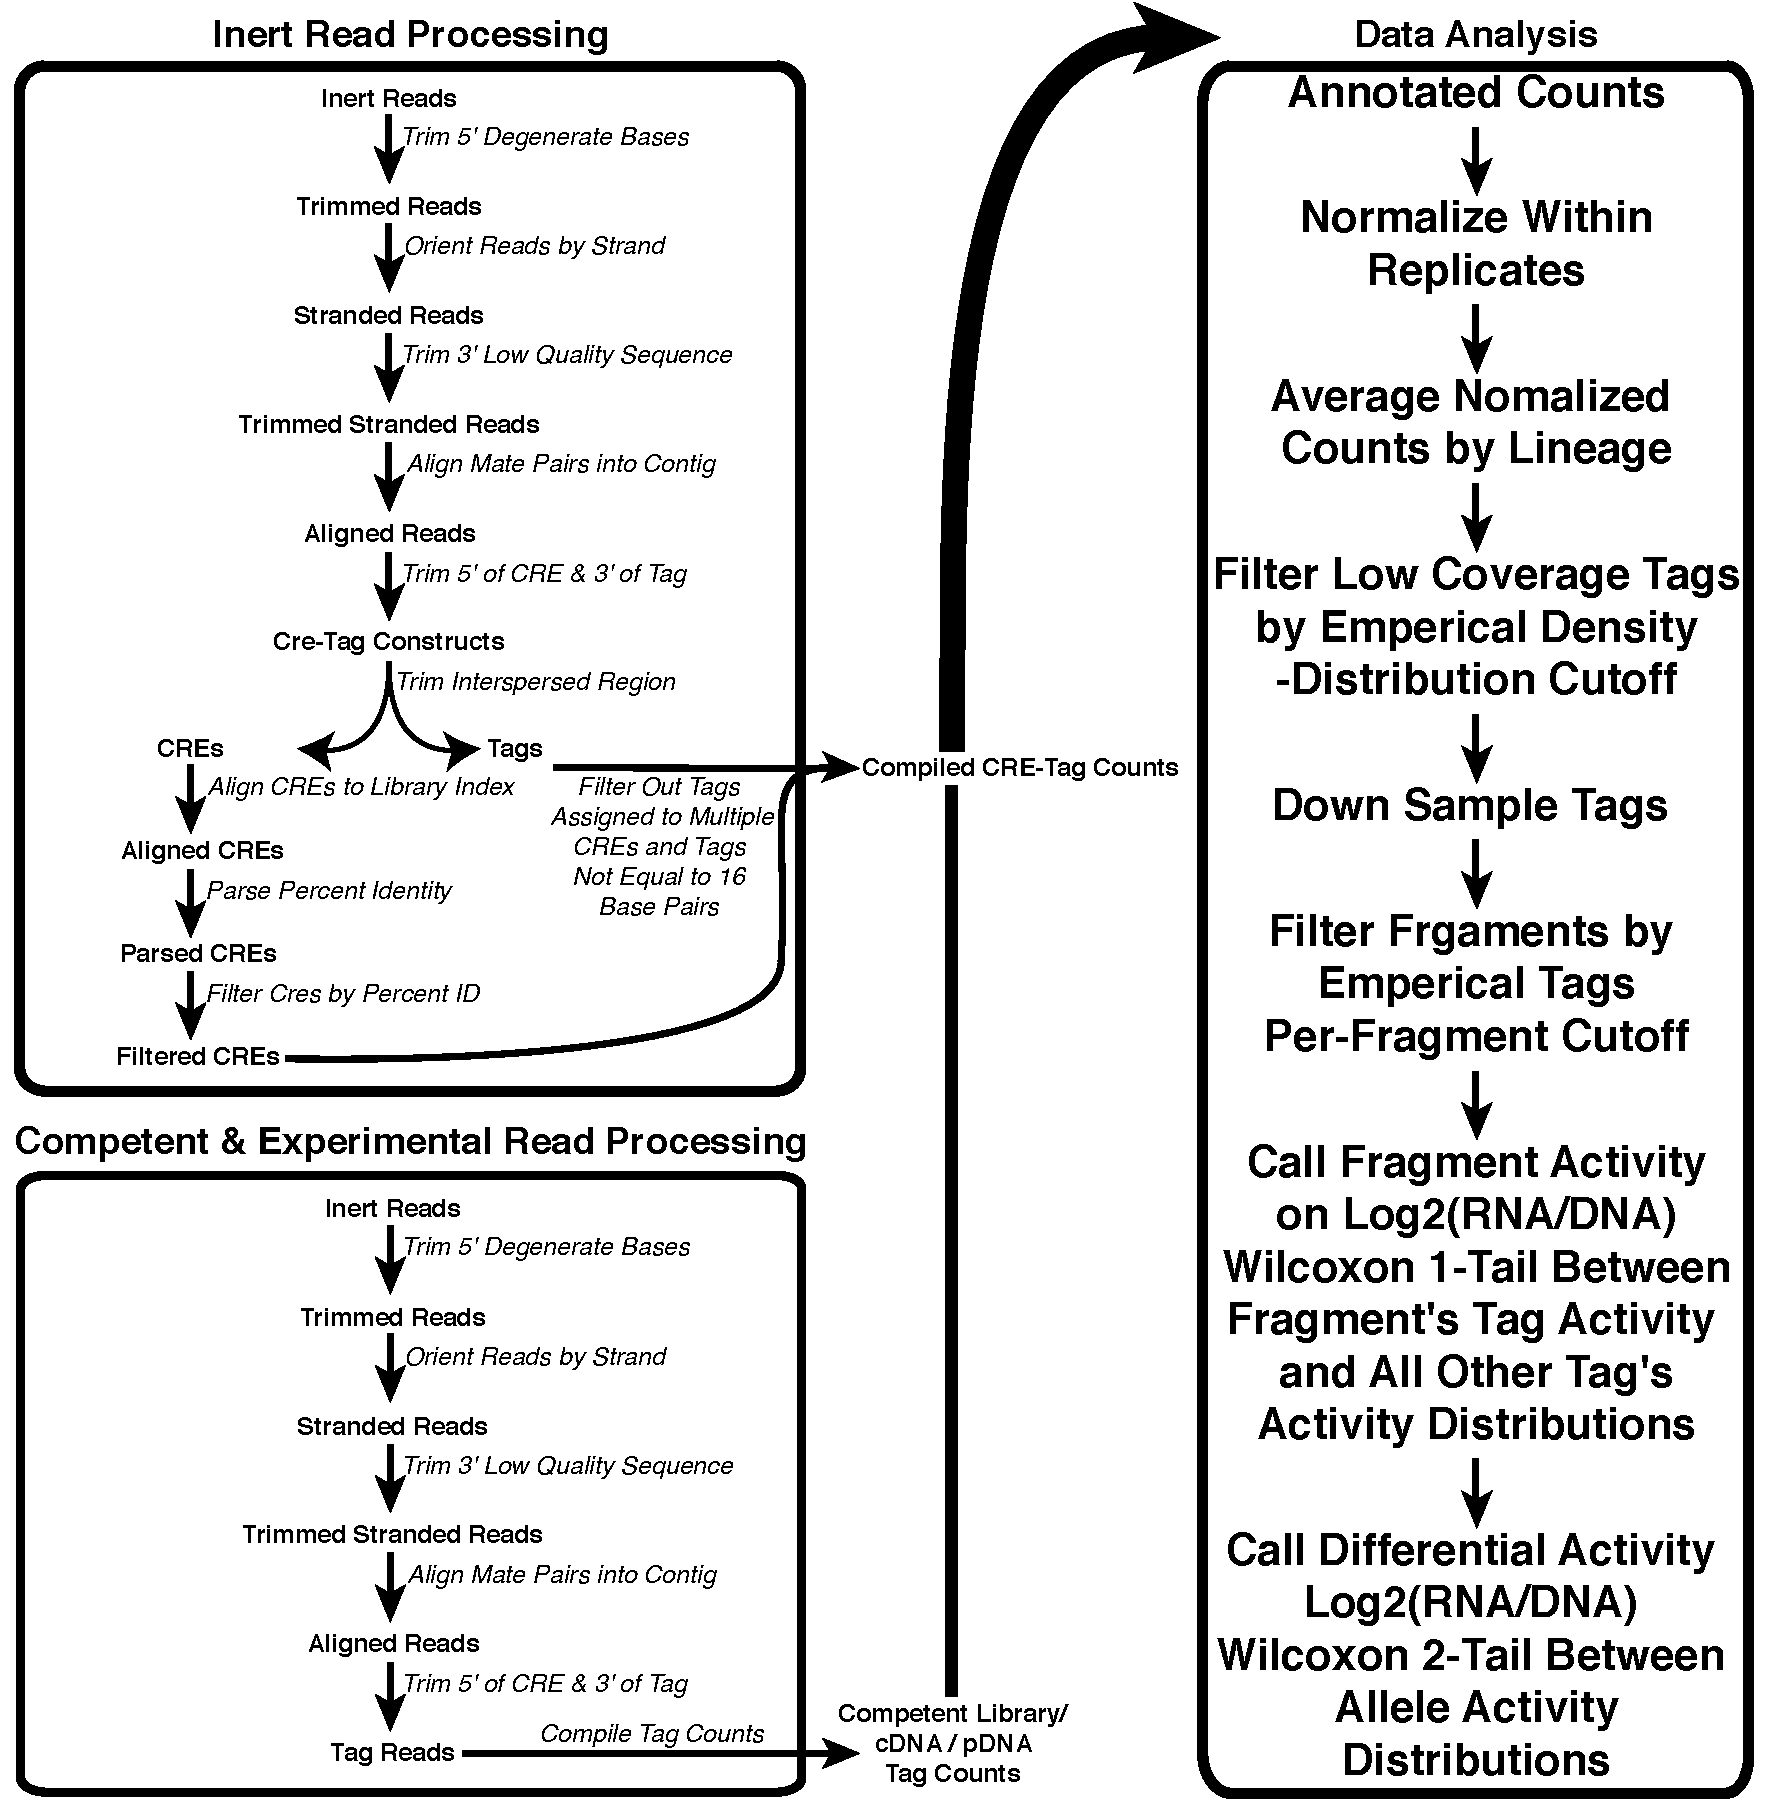
\includegraphics[width=.72\linewidth, keepaspectratio=TRUE]{MPRA_Figures/DataProcessingPipelineFig.pdf}
		\end{center}
		\caption{\textbf{MPRA Data Processing \& Analysis}\label{fig:MPRA_Data}}
			\textbf{Upper Left:} Reads are processed from raw fastq reads into tag and CRE sequences in fastq format. CRE sequences are then aligned to the library index and restricted to user designated threshold of percent identity to the aligned library element. CREs which pass the percent ID threshold are re-annotated with their corresponding tags by read ID and tag entries corresponding to tags which map to multiple CREs or are not 16bp long are filtered form the final data set. \textbf{Lower Left:} Reads of the competent library or experimental reads from plasmid or cDNA fraction are processed similarly to the inert reads an then trimmed into fastq file of tag sequences. Tags are then tabulated into counts and tags not 16bp long are filtered out. \textbf{Center:} The pipelines annotation feature retrieves inert, competent, and all specified experimental files into a single annotated file by tag sequence. Tags missing a count in a given sample are assigned a zero value. Unrepresented fragments are represented by a single line with tag sequence column set to NA and all count columns set to NA. \textbf{Right:} Annotated counts file from the read processing pipeline was processed in R. Tag counts were normalized to CPM, log2 adjusted, activities were calculated as a fold change log2(transcript)/log2(plasmid). Activities were averaged over lineage replicates. Low coverage tags were excluded empirically based on deviation from the population density distribution of tag counts. Low coverage fragments were excluded empirically based on activity correlation in tag down-sampling within fragments at given tag coverage amounts. Activity was called on fragments which passed QC utilizing tags which passed QC with a one-tailed Wilcoxon Rank-Sum Test of fragment tag activity distribution values versus tag activity distribution values of all other tags. Differential activity between orthologous alleles were called on alleles which were paired after QC utilizing a two-tailed Wilcoxon Rank-Sum Test between the allelic tag activity distributions. 
            
	\end{figure}       
    \clearpage
}\normalsize
\clearpage

\section{Results:}
	\subsection{STARR-Seq:}
		\subsubsection{Prospective Analysis}
	
    The first prospective analysis was to examine the existing STARR-Seq data for its robustness at lower read sampling to asses its potential for handling an input DNA source on the scale of the human genome. The data utilized for this analysis was produced by \cite{Arnold:2013aa} utilizing the Drosophila genome as input. The \textit{Drosophila melanogaster} genome 20 times smaller than the human genome. Given that the total sequenced reads of Arnold, \textit{et. al.} was approximately 53.3 and 52.6 million reads for input and transcript fractions, respectively, our targeted sequencing of a full lane’s worth of paired end sequencing (~200 million reads)  places a genomic sized library at a 5-6 times read deficit comparatively. Ignoring the advantage of increasing overall coverage as a function of insert size, we down-sampled this read data to 31, 20, and 10 percent to be thoroughly conservative. Down-sampled reads replicated peak calls of the original data with high fidelity. At ten percent of the original read density, peaks were called across enhancer (inter/intra-genic) regions, promoters, and exonic regions with 76.78\%, 81.42\%, and 77.21\% reproducibility, respectively. Furthermore the amount of new peak calls, resulting presumably from noise, was relatively minimal with the most new peak calls comprising 15\% of the enhancer peak calls from 10\% of the data (Table \ref{STARR_DownSamplePeaks}). 
		
	The 5\% disparity in peak replication raised an important issue on how peak calling on lower coverage data-sets changes by functional peak class. The primary concern being that enhancer peaks may have less read density than promoters opening up the possibility that promoter signal if strong enough could throttle the assay’s dynamic range, effectively drowning out signal from enhancer based reads. By contrast to this concern the distributions of fold change signal between peaks in enhancers and promoters is highly similar if not nominally favoring higher signal in enhancer’s than promoters (Figure \ref{EnhVPromot}). However this result didn’t align with the down sampling peak replication result of a minor decrease of enhancer peaks relative to those with in a promoter. Looking at this distribution as a function of a percent cutoff yielded that the population of enhancer peaks has a much wider dynamic range (Figure \ref{LOGEnhVPromot}). So while the lower end of peaks lost in down-sampling was heavier on enhancers relative to promoters, promoters will most likely not dominate the read space as enhancer peaks are distributed across promoter signal enrichment's and populate the higher end of the distribution as a greater percent of their relative population compared to peaks in promoters.
	
	The final prospective analysis preformed was whether or not it was feasible to transfect a human genomic library into cells and attain a high rate of coverage across the library. The requirements to do this with a reasonable amount of cells are dependent primarily on the multiplicity of the transfection, essentially how many plasmids per-nucleus are transfected. Genomic coverage was estimated as a function of transfection efficiency of 10 million cells for mean values of plasmid transfect per-transfected cell for a multiplicity of 1, 2, 5, and 10 plasmids per-cell (Figure \ref{Multi}). Fragment sizes were estimated to be 500bp. assuming a transfection rate of 20-60\% the target multiplicity to attain reasonable coverage is 10 or more plasmids per-transfected nucleolus. This coverage estimate is an ideal rate coverage estimate, in the sense that it assumes non-overlapping reads, in reality the input library fragments will overlap by a function of their amount and length according to the Poisson distribution. When accounting for this overlap a genomic library can easily cover 99\% of the genome with at least one read at a multiplicity of 5-10 plasmids per-transfected cell and a transfection efficiency of 30-60\% (Figure \ref{Poisson_Multi}). These preliminary projections infer that the STARR-Seq method should be readily tractable in the context of interrogating the entire human genome. 

		\subsubsection{Library Construction \& Quality Control:}

	Individual libraries were constructed from human, mouse, and rhesus BAC DNA input (previously discussed) as well as 2 replicates of human 12878 genomic DNA, 2 replicates of human GM18505 genomic DNA, 2 independent chimpanzee lymphoblastoid cell lines (S0083612, S0083622), and 2 independent rhesus lymphoblastoid cell lines (AG08313, AG08324). All cell lines were female to ensure consistent diploid coverage across Chromosome X, this was done in order to prevent any difficulties in peak calling across the X-Chromosome and because Chromosome Y is largely unalignable. Primate cell lines were checked to ensure that individuals were unrelated. Increasing the diversity between genomic materials within species was intentional as within species diversity aides in resolving functional population variation from functional species variation. All library preparations were run on a 1\% agarose gel at three stages of processing to confirm, proper sonication, size selection and PCR to add Gateway homology arms (Figures \ref{Genomic_Preps} \& \ref{GenomeAndBAC_Preps}). Libraries were cloned into the STARR-Seq vector and grown in batch culture to propagate amplify the library. Before culturing a dilution series of the pooled recovered transformed \textit{E.coli} was plotted to estimate the total complexity of the final library (Table \ref{STARR_LibCov}).
    
	One genomic library and al three BAC libraries were subjected to spot sequencing to analyze library coverage. Both human and Rhesus BAC libraries had unimodal, normally distributed of fragment sizes. The mouse BAC library had a slight shoulder on the low end around 200bp, while the human genomic library had a significant low en shoulder around 200bp (Figure \ref{SpotSeq}). BAC library coverage was plotted as a density distribution across individual BACs within libraries (Figures \ref{hBAC_Dep}, \ref{mBAC_Dep}, \& \ref{rBAC_Dep}). Several BACs were at noticeably low coverage, particularly CH250-321N24, and sections of RP11-205D23. While depth of coverage across most BAC regions followed a unimodal normal distribution there were instances of bimodal normal distribution across some BACs, these situations arise from an additive effect in regions where 2 BACs overlap (Figure \ref{Additive}). While the BAC libraries attained sequencing coverage well into hundreds and over 97\% of the every BAC, except CH250-320P17 was covered (Figures \ref{hBAC_COV}, \ref{mBAC_COV}, \& \ref{rBAC_COV}), The genomic library had a total of 4.90 bases called for an ideal coverage estimate of 1.48x. With the Poisson correction this level of sequencing is expected to cover 77.32\% of the genome with at least one read. The sequencing coverage across the genome was largely equal excluding unalignable sections, and around 70-85\% of all bases were consistently covered (Figure \ref{STARR_Genome_Circos}). This was reinforced by bin analysis dividing the genome into 10Kb bins. This resulted in a unimodal distribution with a mean around 77\% and marginal lower bound tail (Figure \ref{STARR_Genome_STATS}). qPCR was used to assay copy unique transcript molecule copy number after mRNA isolation, cDNA synthesis, and second strand synthesis. These results yielded an estimated unique molecule number of 3-10 million (Figure \ref{CoppNumbProb}).

		\subsubsection{Human Genomic STARR-Seq}

	Genomic library GM12878\_v1 was transfected into GM12878 lymphoblastiod cells in ten electroporation batches of 1 million cells and 1\textmu g of plasmid library. Resulting cDNA and DNA fractions were sequenced on Illumina Hi-Seq 2000’s and 2x76bp read length. Total read depth was 52.2 and 87.4 million reads for plasmid and transcript fractions respectively. The alignable read percentages were 78.8\% and 76.4\% respectively. Fragment length between fractions did not differ significantly (Figures \ref{pDNA_InputSize} \& \ref{TransFragSize}). Calling peaks with an in house peak caller \cite{Reilly:2015aa} yielded 673 peak calls. Twenty of these peaks intersected know promoters as defined by the UCSC gene set, and 49 overlapped with know enhancers in the 9 primary ENCODE cell lines. This seemed like a low amount of functional overlap. Although it’s not unexpected that some repeats will drive transcription in the episomal context characteristic of the STARR-Seq assay, this low amount of overlap seemed worrisome. Upon analysis of some example peaks from this pilot experiment it was evident that the signal produced was driven by expected genomic factors such as transcription factor binding peaks in acetylated promoters and suspected enhancers (Figures \ref{GENOME_Pro} \& \ref{GENOME_Enh}). 
    
	What is strikingly noticeable from figures \ref{GENOME_Pro} \& \ref{GENOME_Enh} is the blocky nature of the transcript signal and input signal, inferring that the coverage of these peaks is low. Overall low coverage in this enrichment analysis may be the route cause of spurious peaks being called as a result of low input coverage. To this end analysis of the plasmid fraction yielded interesting results. Given the average fragment length of 472bp (Figure \ref{pDNA_InputSize}) and the percent of reads across chromosomes, we expect an ideal coverage of  approximately 4.75-6.75x across all autosomes and the X-Chromosome. After Poisson correction for overlap we would expect to lack any coverage of between 1-0.09\% of bases. Instead coverage analysis from aligned reads resulted in 52.3-33.2\%. While the high end is driven by acentric chromosomes with large spans of unalignable sequences such as chromosome 22, the vast majority of autosomes as well as chromosome-X show coverage gaps of 32-40\%, which is consistent with an ideal coverage estimate of 1x (Table \cite{GenomeCov}). The foundation of this disparity lies in the amount of unique reads within the input data set. Filtering for unique reads resulted in only seven million unique reads, at an average length of 472bp the total bases covered by unique reads is 3.3 billion bases, equating almost exactly for a 1x ideal coverage. This lack of fragment diversity was also investigated within the transcript fraction. Normally in transcription based assay such as STARR-Seq low levels of PCR duplication can be tolerated within the transcript fraction as it is assumed to be a product of transcription, however when molecule diversity is so low, in the transcript as well as the plasmid input this assumption is no longer valid. This transcript is expected to be amplified in the transcript fraction as the total number of molecules isolated is estimated to be on the order of 100-fold less by qPCR (Figure \ref{CoppNumbProb}). Indeed the transcript fraction only contained 140,000 unique reads. The fraction specific PCR of 10-14 cycles followed by 10 rounds of amplification with the illumina primers was expected to be the root cause of this issue. 
	
		\subsubsection{Human BAC Experiment}
	
	With the previous results in mind STARR-Seq was modified in several ways to robustly investigate its feasibility in mammalian systems. The first was optimizing the primer concentrations for fraction specific amplification. The target being to amplify a set number of constructs with a concentration of primers optimized to be the most efficient at amplifying the template in relatively few cycles without producing primer dimers or other secondary products (Table \ref{TransPCRA}). The second step was to optimize cDNA synthesis methods through comparison of custom strand specific, oligo-dt, and random hex priming strategies. This resulted in a custom strand primer exhibiting a nominally greater capacity for transcript priming realative to oligo-dt (Figure \ref{cDNA_Synthesis_Strategies}). The third alteration in the STAR-Seq Library was to create parallel hBAC libraries with a minimal promoter commonly used for enhancer assays in the PGL 4.73 vector series, as well as a third version utilizing a more robust SV40 promoter. Coupled with the hBAC library driven by the original synthetic SCP1 promoter \cite{Arnold:2013aa},  these variant-promoter driven libraries should yield insight on whether the STARR-Seq library can produce enough signal to produce the heterogeneity of fragments within peaks to robustly call high-confident peak enrichments. 

	Despite these alterations, the issue of lowered diversity was not ameliorated within the hBAC library experiment conditions or between promoter variants (Table \ref{hBAC_Reads}). Both SV-40 and minP promoters were less robust in expression capacity than the synthetic SCP1 STARR-Seq promoter. The read length distributions were unimodal, normally distributed, and highly similar between fraction and promoter-variant libraries for each library. The maximum difference between mean fragment lengths of either fraction in any promoter variation was only 18bp (Figure \ref{AbsFragSize}) and fragment length didn't differ between fractions within called peaks \ref{FraginPeak}. Although the unique read counts were lower than optimal reads fractions were analyzed for transcript enrichment through two independent methods. The first was a windowing ChIP-Seq enrichment peak calling script used previously, and the second was an adaptation of the method utilized in previous STARR-Seq analysis in Drosophila \cite{Arnold:2013aa}. This adaptation calculates transcript enrichment with 350bp windows across the hBAC libraries at 175bp intervals and calls the upper 10\% of enriched windows peaks instead of applying an intrinsically adjusted p-value based on window comparisons. The theory around this enrichment method was that it could help in restricting peak length inflation that may result from inflated p-values around true peaks based solely on low coverage within the input fraction.
	
    hBAC peaks were called with both methods for all three promoter variants (Table \ref{PeakCalls}) and were overlapped pairwise between the six conditions (Table \ref{PeakOverlaps}). As expected, percent of overlapping peaks tend to be highest between calling methods of promoter variants. The one exception to this is between SCP1 promoter driven peak calling methods. The disparity of overlap between percent of overlapping peaks between calling methods may as a result of the peak size distributions resulting from peak calling methods. The ChIP-Seq peak caller had a much larger tail of longer peaks (Figure \ref{ Windower_PeakSize}) than the enrichment based method (Figure \ref{ STARk_PeakSize }). This could be the result of increased sensitivity versus specificity for the ChIP seq calling method compared to the enrichment method, or a combination of this theory and an inability of the peak calling ChIP seq script to adequately handle the lack of library coverage.
	
    Fold enrichment of bases peak regions reveal lower than expected fold enrichment values of transcript enrichment over plasmid input (Figure \ref{Wind_BaseEnrich}). Peak enrichment was calculated and normalized to peak length and compared to length normalized enrichment within non-enriched regions for the ChIP-Seq Peak caller (Figure \ref{Norm_Wind}) and the 350bp windowing enrichment method (Figure \ref{Norm_Stark}). This produced an relative enrichment for peaks within higher fold change range, particularly the 350bp windowed method for the MinP and SV40 promoter library variants. However given the high degree of overlap between peaks and non-enriched regions of the library the distribution of transcript reads was analyzed for coverage inside versus outside peaks. Peaks of the same size and amount for each BAC region were permuted randomly and intersected with reads from the respective BAC 10,000 times. For each permutation the percent of total reads within permuted peak regions were recorded. The percent of total reads which fall within actual called peaks served as out observed values to compare to the permuted distributions. Enrichment of transcript reads within called peaks was highly significant for both peak calling methods and all promoter variants compared to enrichment distributions within randomly permuted peaks (Figures \ref{Window_Perm} \& \ref{STARK_Perm}). This enrichment of signal serves diagnostically to confirm that both peak calling methods are correctly identifying the enriched regions of signal from the hBAC libraries. 
	
    To examine peak calling methods and promoter variant hBAC peaks for signal specificity, peaks were randomly permuted as before and intersected with H3K27Ac peaks and DNAse hypersensitivity regions from 9 ENCODE cell lines. Compared to the observed peak overlaps this analysis yields a view on how well the hBAC data replicates expected \textit{apriori} active regions within the genome. As the hBAC library is present within the GM12878 cell line in an episomal context it is expected that any region capable of interacting with the trans environment can produce signal regardless of it’s chromatin context within the GM12878 genome. This analysis revealed quite a few enrichments within H3K27Ac enriched regions and DNAse Hypersensitivity regions from the analyzed cell lines (Figures \ref{H3K27AcPerms} \& \ref{DNAsePerms}), however no specific cell line or promoter variant exhibited a clear signal of overlap relative to others across both data sets. A representative peak from the enriched 350bp windowing technique shows the potential power of the STARR-Seq assay to read out sequences which drive transcription (Figure \ref{STARR_Peak}).
	
%Down Sampling 
\afterpage{
	\renewcommand{\arraystretch}{1.1}%
	\begin{table}[p]
		\begin{center}
			\scalebox{1}{
            \begin{tabular}{c|cccc}

	Functional Region	& 	100\% 	& 	31\%	& 	20\%	& 	10\%	\\\hline

	Enhancer	& 	2450 	& 	2377	& 	2326	& 	2217	\\
	Promoter	& 	1168 	& 	1176	& 	1124	& 	1050	\\
	Exonic		& 	535 	& 	537		& 	522	& 	490	\\
				\\\\
	Functional Region	& 	100\% 	& 	31\%	& 	20\%	& 	10\%	\\\hline

	Enhancer	& 	2450 	& 	2115	& 	2015	& 	1881	\\
	Promoter	& 	1168 	& 	1093	& 	1026	& 	951	\\
	Exonic		& 	535 	& 	475		& 	444	& 	413	\\
\\\\

	Functional Region	& 	100\% 	& 	31\%	& 	20\%	& 	10\%	\\\hline

	Enhancer	& 	- 	& 	86.65\%	& 	82.65\%	& 	76.78\%	\\
	Promoter	& 	- 	& 	93.58\%	& 	87.84\%	& 	81.42\%	\\
	Exonic		& 	- 	& 	88.79\%	& 	82.99\%	& 	77.21\%	\\
				\end{tabular}
                }
			\caption{\textbf{Down-Sampling Drosophila Reads }}
			\label{STARR_DownSamplePeaks}
            \begin{flushleft}Reads were randomly down-sampled to 31\%, 20\%, and 10\% of the original number. Enriched peaks were call on each set and binned according to genomic context of whether the peak overlapped with a promoter, an exon, or was inter/intra-genic. \textbf{Top: }Total number of peaks called. \textbf{Middle: }Number of replicated peaks called. \textbf{Bottom: }Percent of replicated peaks called. \end{flushleft}
		\end{center}
	\end{table}
	\clearpage
}\normalsize

%Perspective Analysis Signal Enhancers vs Promoters
\afterpage{
	\begin{figure}[p]
		\begin{center}
			\includegraphics[width=1\linewidth, keepaspectratio=TRUE]{STARR_Results/Promoter_v_Intergenic.png}
		\end{center}
		\caption{\textbf{ Intensity of Signal in Drosophelia STARR-Seq Peaks}} 
        \label{EnhVPromot}
        \begin{flushleft}Distribution of Log2 fold enrichment of Drosophila STARR-Seq peaks for peaks within promoters versus intergenic peaks.\end{flushleft}
	\end{figure}       
    \clearpage
}\normalsize 

%Perspective Analysis Promoters Versus Intergenic
\afterpage{
	\begin{figure}[p]
		\begin{center}
			\includegraphics[width=1\linewidth, keepaspectratio=TRUE]{STARR_Results/Percent_above_threashold_log2.png}
		\end{center}
		\caption{\textbf{ Intensity of Signal in Drosophelia STARR-Seq Peaks By Population }}
        \label{LOGEnhVPromot}
        \begin{flushleft}Percent of Drosophila STARR-Seq peaks above Log2 fold enrichment for peaks within promoters versus intergenic peaks. \end{flushleft}
	\end{figure}       
    \clearpage
}\normalsize 

%Perspective Analysis Multiplicity
\afterpage{
	\begin{figure}[p]
		\begin{center}
			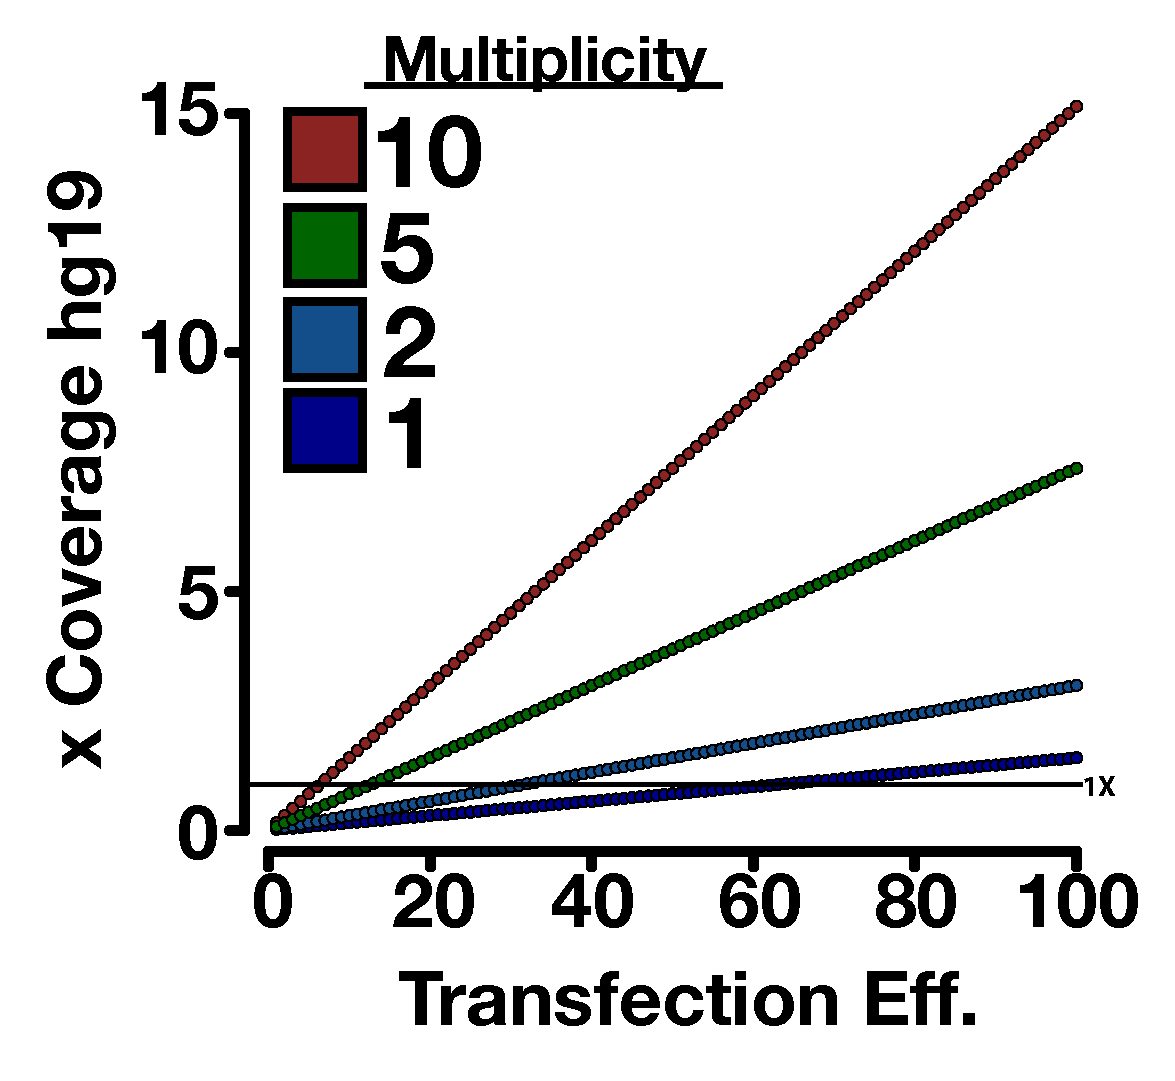
\includegraphics[width=1\linewidth, keepaspectratio=TRUE]{STARR_Results/10_Million_Cells_TransEFF_Multiplicity.pdf}
		\end{center}
		\caption{\textbf{Projected Restraints of Genomic-Scale Library} }
        \label{Multi}    
       \begin{flushleft}Estimated genomic coverage as a function of transfection efficiency for differing levels of average plasmids per-nucleous transfected. \end{flushleft}
	\end{figure}       
    \clearpage
}\normalsize    

%Perspective Analysis Poisson Gaps
\afterpage{
	\begin{figure}[p]
		\begin{center}
			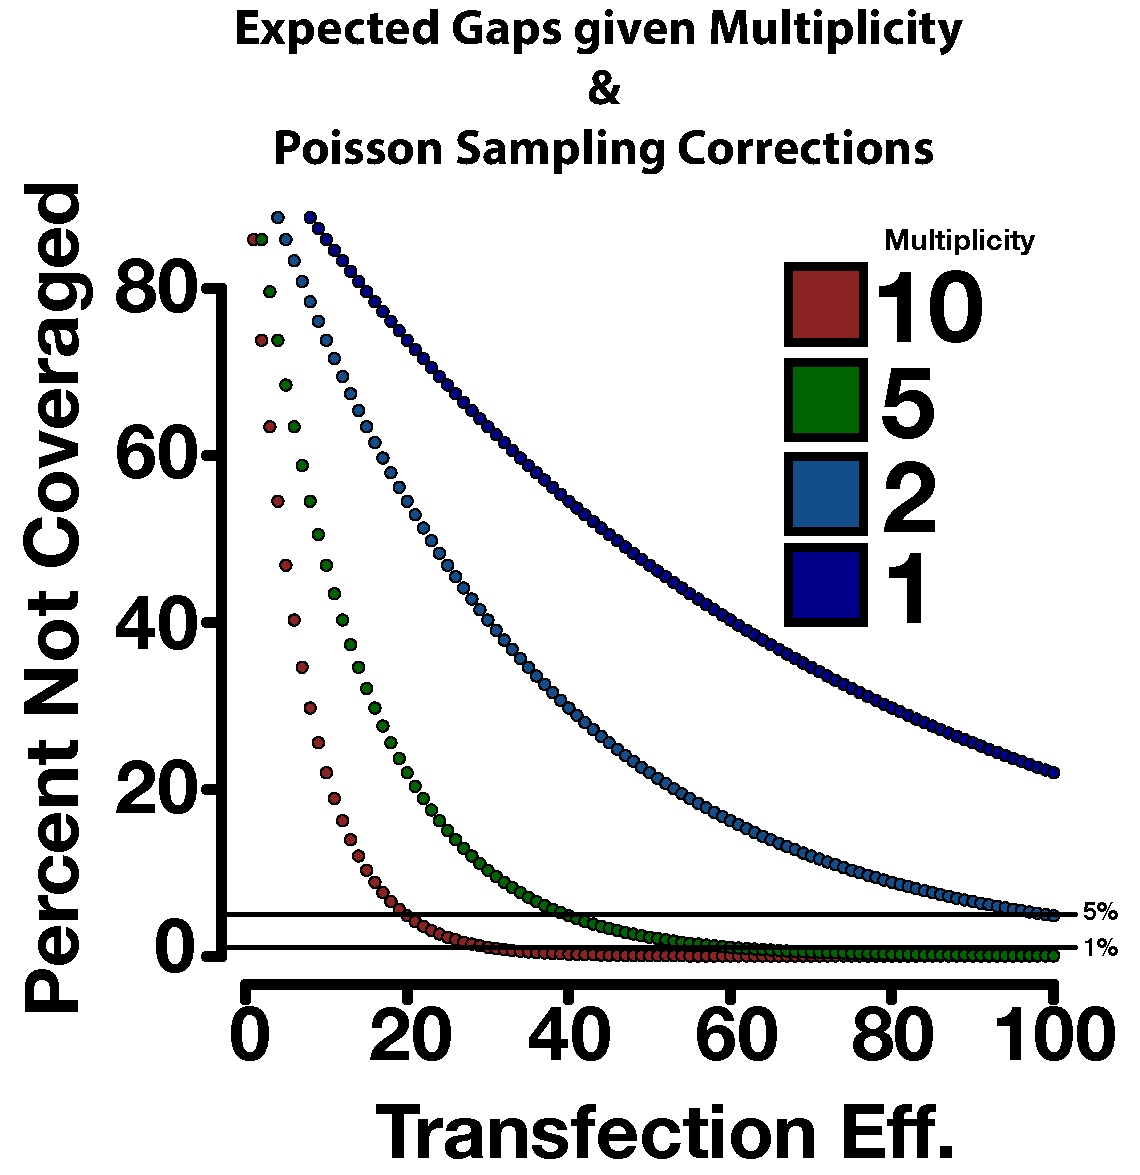
\includegraphics[width=1\linewidth, keepaspectratio=TRUE]{STARR_Results/10_Million_Cells_TransEFF_Poisson.pdf}
		\end{center}
		\caption{\textbf{Poisson Corrected Genomic-Scale Library Projection}} 
        \label{Poisson_Multi}
		 \begin{flushleft}Pisson corrected estimate of gaps in genomic coverage as a function of transfection efficiency for differing levels of average plasmids per-nucleous transfected. \end{flushleft}
    \end{figure}       
    \clearpage
}\normalsize  

%QC Genomic Libarary Preps
\afterpage{
	\begin{figure}[p]
		\begin{center}
			\includegraphics[width=1\linewidth, keepaspectratio=TRUE]{STARR_Results/2014_10_21_All_Genomic_Lib_PrepsSmall.png}
		\end{center}
		\caption{ \textbf{ Genomic STARR-Seq Library Preps } }
        \label{Genomic_Preps}
        \begin{flushleft}Genomic DNA isolated from lymphoblast cell lines were used to prepare Genomic Scale STARR-Seq libraries from two human populations, CEU and YRI in duplicate as well as from 2 Chimpanzee lines and 2 Rhesus lines. Three primary rounds of quality control were preformed through out library prep. \textbf{1) } Sonicated genomic DNA was run to check the initial fragment size distribution. \textbf{2) } Adapter ligated and size selected fragment library was run to confirm desired fragment size range. \textbf{3) } PCR amplified library was run to confirm library size increase as a product of adding the cloning arms of the library via tailed primers. DNA size ladders in each panel indicate 1kB (\textit{Left}) and 100bP (\textit{Right}.\end{flushleft}
	\end{figure}       
    \clearpage
}\normalsize   

%QC BAC Libs
\afterpage{
	\begin{figure}[p]
		\begin{center}
			\includegraphics[width=1\linewidth, keepaspectratio=TRUE]{STARR_Results/All_Library_Preps_Print.pdf}
         	
		\end{center}
		\caption{ \textbf{ Genomic and BAC Libraries } }
        \label{GenomeAndBAC_Preps}
        \begin{flushleft}Genomic DNA isolated from lymphoblast cell lines and BAC DNA were used to create a human genomic and 3 orthologus BAC libraries from human, mouse, and rhesus BACs. Three primary rounds of quality control were preformed through out library prep. The human genomic example is from Figure \ref{Genomic_Preps}, left most GM12878 library prep. \textbf{1) } Sonicated genomic DNA was run to check the initial fragment size distribution. \textbf{2) } Adapter ligated and size selected fragment library was run to confirm desired fragment size range. \textbf{3) } PCR amplified library was run to confirm library size increase as a product of adding the cloning arms of the library via tailed primers. DNA size ladders in each panel indicate and 100bP scale ladder.\end{flushleft}
	\end{figure}       
    \clearpage
}\normalsize 

%QC Library Coverage
\afterpage{
	\renewcommand{\arraystretch}{1.1}%
	\begin{table}[p]
		\begin{center}
			\scalebox{1}{
            \begin{tabular}{c|cccc}

	BAC Library or Cell-Line	& 	Coverage	\\\hline

	hBAC	& 	39.4x 	\\
	rheBAC	& 	17.4x	\\
	mBAC	& 	5x		\\

	GM12878\_V1	& 	9.6x 	\\
	GM12878\_V2	& 	47.3x	\\
	GM18505\_V1	& 	40.6x		\\
    GM18505\_V2	& 	30.5x 	\\
	S003612	& 	33.1x	\\
	AG08312	& 	40.7x		\\

				\end{tabular}
                }
			\caption{\textbf{STARR-Seq Library Coverage}}
			\label{STARR_LibCov}            
		\end{center}
	\end{table}
	\clearpage
}\normalsize

%QC Spot Sequencing Fragment Size
\afterpage{
	\begin{figure}[p]
		\begin{center}
			\includegraphics[width=1\linewidth, keepaspectratio=TRUE]{STARR_Results/2014_07_03_Lib_Fragment_Dist.pdf}
		\end{center}
		\caption{\textbf{STARR-Seq Library Spot Sequencing Fragment Size}}  			
        \label{SpotSeq}
		\begin{flushleft}Histograms of the fragment size distribution of the spot-sequencing preformed on the initial library construction of the (\textit{From left to right}) Human genomic, human BAC, mouse BAC, and rhesus BAC libraries) \end{flushleft}
    \end{figure}       
    \clearpage
}\normalsize  

%human BAC depth
\afterpage{
	\begin{figure}[p]
		\begin{center}
			\includegraphics[width=1\linewidth, keepaspectratio=TRUE]{STARR_Results/hBAC_Norm_per.pdf}
		\end{center}
		\caption{\textbf{hBAC Library Coverage Depth}} 
        \label{hBAC_Dep}
        \begin{flushleft}Histograms of each BAC coordinate region are plotted as a density plot of coverage by base pair. Most BACs have normal uni-modal distributions with the exception of those experiencing additive coverage affects from overlap with another BAC. One BAC, RP11-205D23 is at a particularly low coverage relative to the other BAC regions. \end{flushleft}
	\end{figure}       
    \clearpage
}\normalsize 

%human BAC Coverage
\afterpage{
	\begin{figure}[p]
		\begin{center}
			\includegraphics[width=.78\linewidth, keepaspectratio=TRUE]{STARR_Results/Extended_Human_BACs_Thesis.pdf}
		\end{center}
		\caption{\textbf{hBAC Library Coverage Plot}} 
        \label{hBAC_COV}
        \begin{flushleft} Coverage depth across each base in the human BAC library. The total percent of bases within each BAC region covered by at least one read is reported as \textit{'Cov ='}. \end{flushleft}
	\end{figure}       
    \clearpage
}\normalsize 


%mouse BAC depth
\afterpage{
	\begin{figure}[p]
		\begin{center}
			\includegraphics[width=1\linewidth, keepaspectratio=TRUE]{STARR_Results/mBAC_Norm_per.pdf}
		\end{center}
		\caption{\textbf{mBAC Library Coverage Depth}}
        \label{mBAC_Dep}
        \begin{flushleft}Histograms of each BAC coordinate region are plotted as a density plot of coverage by base pair. \end{flushleft}
	\end{figure}       
    \clearpage
}\normalsize 

%Mouse BAC Coverage
\afterpage{
	\begin{figure}[p]
		\begin{center}
			\includegraphics[width=1\linewidth, keepaspectratio=TRUE]{STARR_Results/mExtended_Thesis.pdf}
		\end{center}
		\caption{\textbf{mBAC Library Coverage Plot}} 
        \label{mBAC_COV}
        \begin{flushleft} Coverage depth across each base in the mouse BAC library. The total percent of bases within each BAC region covered by at least one read is reported as \textit{'Cov ='}.\end{flushleft}
	\end{figure}       
    \clearpage
}\normalsize 

%Rhesus BAC depth
\afterpage{
	\begin{figure}[p]
		\begin{center}
			\includegraphics[width=1\linewidth, keepaspectratio=TRUE]{STARR_Results/rBAC_Norm_per.pdf}
		\end{center}
		\caption{\textbf{rBAC Library Coverage Depth}} 
        \label{rBAC_Dep}
        \begin{flushleft}Histograms of each BAC coordinate region are plotted as a density plot of coverage by base pair. Most BACs have normal uni-modal distributions with the exception of those experiencing additive coverage affects from overlap with another BAC. One BAC, CH250-401G11-205D23 is at a particularly low coverage relative to the other BAC regions. \end{flushleft}
	\end{figure}       
    \clearpage
}\normalsize 

%Rhesus BAC Coverage
\afterpage{
	\begin{figure}[p]
		\begin{center}
			\includegraphics[width=.9\linewidth, keepaspectratio=TRUE]{STARR_Results/rExtended_Thesis.pdf}
		\end{center}
		\caption{\textbf{rBAC Library Coverage Plot}}
        \label{rBAC_COV}
        \begin{flushleft} Coverage depth across each base in the rhesus BAC library. The total percent of bases within each BAC region covered by at least one read is reported as \textit{'Cov ='}.\end{flushleft}
	\end{figure}       
    \clearpage
}\normalsize 

%Additive Coverage Issue
\afterpage{
	\begin{figure}[p]
		\begin{center}
			\includegraphics[width=1\linewidth, keepaspectratio=TRUE]{STARR_Results/Additive_increase.pdf}
		\end{center}
		\caption{ \textbf{Additive Coverage Increase As a Function of BAC Overlap} } 
        \label{Additive}
        \begin{flushleft}BAC coordinates tend to overlap within libraries creating an additive effect on coordinate coverage within overapping intervals.\end{flushleft}
	\end{figure}       
    \clearpage
}\normalsize 

%QC Genomic Library Circos
\afterpage{
	\begin{figure}[p]
		\begin{center}
			\includegraphics[width=1\linewidth, keepaspectratio=TRUE]{STARR_Results/Genomic_Lib_CoverageFinal.png}
		\end{center}
		\caption{\textbf{Genomic Library Coverage}} 
        \label{STARR_Genome_Circos}
        \begin{flushleft}Spot sequencing coverage of the STARR-Seq library, by chromosome. Each concentric level represents a histogram, with the exception of the second band from the inside which represents each chromosome's banding pattern. Bin's represent 10,000 base pair steps. The inner histogram (red) represents gaps in sequencing coverage from outside (o\%) to inside (100\%). The second from the outside represents sequence coverage (green) from inside (0\%) to (100\%) and unalignable sequence (blue) from outside (0\%) to inside (100\%). Percent of repetitive sequence is represented in the outside histogram (purple) from inside (0\%) to outside (100\%). \end{flushleft}
	\end{figure}       
    \clearpage
}\normalsize 

%QC Genomic Library sequencing Stats
\afterpage{
	\begin{figure}[p]
		\begin{center}
			\includegraphics[width=1\linewidth, keepaspectratio=TRUE]{STARR_Results/Genome_statsV2.pdf}
		\end{center}
		\caption{\textbf{Genomic Coverage Statistics by Bin}}
        \label{STARR_Genome_STATS}
        \begin{flushleft}Covereage Statistics by bin (10,000 bases per-bin) of Figure \ref{STARR_Genome_Circos}. Percent of bases covered by at least one read as each 10kb bin across the human genome. \end{flushleft}
	\end{figure}       
    \clearpage
}\normalsize 

%QC Transfection?Copy number Problem
\afterpage{
	\begin{figure}[p]
		\begin{center}
			\includegraphics[width=1\linewidth, keepaspectratio=TRUE]{STARR_Results/2015_15_15_STARR.pdf}
		\end{center}
		\caption{\textbf{ qPCR on STARR-Seq cDNA }}%\label{STARR_qPCR}
        \label{CoppNumbProb}
		\begin{flushleft}qPCR was preformed on purifed plasmid (\textit{Purple}), cDNA synthesized by custom first strand primer synthesis (\textit{Blue}), and No RT contro(\textit{Green}), fractions of a STARR-Seq experiment to assay the total number of unique molecules recovered from a STARR-Seq experiment. \end{flushleft}
    \end{figure}       
    \clearpage
}\normalsize 

%Transfected BAC lib pDNA Frag Size
\afterpage{
	\begin{figure}[p]
		\begin{center}
			\includegraphics[width=1\linewidth, keepaspectratio=TRUE]{STARR_Results/STARR_Seq_experiment_Sequenced_input_Fragment_size_copy.pdf}     
		\end{center}
		\caption{\textbf{Fragment Size of Input STARR-Seq Library}} 
        \label{pDNA_InputSize}
		\begin{flushleft} Histogram of the fragment lengths from the recovered plasmid input fraction of transfecting the human genomic library GM12878\_v1 into GM12878 lymphoblastoid cell line.\end{flushleft}
    \end{figure}       
    \clearpage
}\normalsize 

%Transfected BAC lib Transcript Frag Size
\afterpage{
	\begin{figure}[p]
		\begin{center}
			\includegraphics[width=1\linewidth, keepaspectratio=TRUE]{STARR_Results/STARR_Seq_experiment_SequencedcDNA_all_Fragment_Size_copy.pdf}
		\end{center}
		\caption{\textbf{Fragment Size of cDNA Transcripts}} 
        \label{TransFragSize}
        \begin{flushleft} Histogram of the fragment lengths from the cDNA synthesized from the transcript fraction of transfecting the human genomic library GM12878\_v1 library into the GM12878 lymphoblastoid cell line.\end{flushleft}
	\end{figure}       
    \clearpage
}\normalsize 

%Genomic STARR-Seq Peak - Promoter
\afterpage{
	\begin{figure}[p]
		\begin{center}
			\includegraphics[width=1\linewidth, keepaspectratio=TRUE]{STARR_Results/hgt_genome_7bdc_265980.pdf}
		\end{center}
		\caption{\textbf{Genomic Scale STARR-Seq Promoter Peak}} 
        \label{GENOME_Pro}
        \begin{flushleft} An example of a STARR-Seq signal enriched peak yielded from the genomic scale STARR-Seq transfection. This peak resides within a promoter region as defined by the UCSC gene annotation set. This promoter contains multiple H3K27 acetylated transcrption factor binding sites within an ENCODE characterized cell lines.\end{flushleft}
	\end{figure}       
    \clearpage
}\normalsize 

%Genomic STARR-Seq Peak - Enhancer
\afterpage{
	\begin{figure}[p]
		\begin{center}
			\includegraphics[width=1\linewidth, keepaspectratio=TRUE]{STARR_Results/hgt_genome_2cbe_264bb0.pdf}
		\end{center}
		\caption{\textbf{Genomic Scale STARR-Seq Enhancer Peak}} 
        \label{GENOME_Enh}
        \begin{flushleft} An example of a STARR-Seq signal enriched peak yielded from the genomic scale STARR-Seq transfection. This peak resides within an intergenic region containing H3K27 acetylated transcrption factor binding sites within an ENCODE characterized cell line. \end{flushleft}
	\end{figure}       
    \clearpage
}\normalsize 

%QC Library Coverage
\afterpage{
	\renewcommand{\arraystretch}{1.1}%
	\begin{table}[p]
		\begin{center}
			\scalebox{1}{
            \begin{tabular}{c|cc}

	Chromosome 	&	Estimated Coverage	&	Actual Percent Not Covered	\\\hline
1	&	6.27x	&	37.80\%	\\
2	&	6.65x	&	33.20\%	\\
3	&	6.68x	&	32.50\%	\\
4	&	6.51x	&	34.30\%	\\
5	&	6.60x	&	33.50\%	\\
6	&	6.61x	&	34.50\%	\\
7	&	6.62x	&	33.90\%	\\
8	&	6.71x	&	33.20\%	\\
9	&	5.48x	&	44.90\%	\\
10	&	6.72x	&	33.50\%	\\
11	&	6.75x	&	32.50\%	\\
12	&	6.71x	&	32.50\%	\\
13	&	5.61x	&	43.70\%	\\
14	&	5.68x	&	43.00\%	\\
15	&	5.43x	&	45.70\%	\\
16	&	6.18x	&	39.70\%	\\
17	&	6.73x	&	32.70\%	\\
18	&	6.64x	&	33.70\%	\\
19	&	6.62x	&	32.70\%	\\
20	&	6.21x	&	31.60\%	\\
21	&	5.06x	&	50.00\%	\\
22	&	4.75x	&	52.30\%	\\
X	&	6.14x	&	37.00\%	\\
Y	&	0.04x	&	99.30\%	\\

				\end{tabular}
                }
			\caption{\textbf{Genomic STARR-Seq Input Coverage}}
			\label{GenomeCov}
            
		\end{center}
	
    \begin{flushleft} Table of estimated ideal coverage depth of each chromosome as a function of average read length and the number of reads aligned to each chromosome. GM12878 is a female derived cell line, therefore Chromosome Y is included as a negative control. The actual percent of each chromosome not covered by a single read is reported and corresponds after translation with a Poisson fragment overlap estimate to an ideal coverage of approximately 1x coverage. \end{flushleft}
    \end{table}
	\clearpage
}\normalsize

%Development qPCR
\afterpage{
	\begin{figure}[p]
		\begin{center}
			\includegraphics[width=1\linewidth, keepaspectratio=TRUE]{STARR_Results/2014_07_22_qPCR_mRNA_pDNA_data_copy.pdf}
		\end{center}
		\caption{\textbf{STARR-Seq qPCR Copy Number}}
        \label{cDNA_Synthesis_Strategies}
        \begin{flushleft}qPCR results on cDNA synthesized from isolated GM12878 mRNA 24hours after transfection with competent STARR-Seq library and the corresponding plasmid library DNA fraction. Symbols denote different cDNA  methods used to prime first strand synthesis; Oligo dt (solid fill: $\Diamond$), Random Hexamers (solid fill: $\Box$), Custom Primer (solid fill: $\triangle$), and no reverse transcript control (solid fill: $\circ$). Colors represent different template targets, Beta-Actin Control (Yellow), and GFP STARR-Seq ORF transcript (Blue).\end{flushleft}
	\end{figure}       
    \clearpage
}\normalsize 

%QC Library Coverage
\afterpage{
	\renewcommand{\arraystretch}{1.1}%
	\begin{table}[p]
		\begin{center}
			\scalebox{.9}{
            \begin{tabular}{c|ccccc}
hBAC Library	&	Fraction	&	Reads Processed	&	PE-Alignments	&	Percent Aligned	&	Unique Fragments	\\\hline
STARR	&	Transcript	&	26,310,083	&	20,975,576	&	79.72\%	&	105,529	\\
STARR	&	Plasmid		&	30,787,455	&	24,928,995	&	80.97\%	&	152,052	\\
MinP	&	Transcript	&	39,247,522	&	31,191,779	&	79.47\%	&	16,545	\\
MinP	&	Plasmid		&	39,183,426	&	31,304,076	&	79.89\%	&	312,080	\\
SV40	&	Transcript	&	41,197,959	&	33,139,563	&	80.44\%	&	25,105	\\
SV40 	&	Plasmid		&	30,025,460	&	23,859,957	&	79.47\%	&	382,941	\\
				\end{tabular}
                }
			\caption{\textbf{Human BAC Library Reads}}
			\label{hBAC_Reads}           
		\end{center}	
    \begin{flushleft}For each plasmid and transcript fraction for all three promoter variant hBAC libraries the total amount of reads, amount of successfully paired reads, the percent of alignable reads, and total unique reads are reported. \end{flushleft}
    \end{table}
	\clearpage
}\normalsize


%Sequenced Fragment Lengths
\afterpage{
	\begin{figure}[p]
		\begin{center}
			\includegraphics[width=1\linewidth, keepaspectratio=TRUE]{STARR_Results/Insert_Size_Dist_Final.pdf}
		\end{center}
		\caption{\textbf{Sequenced Fragment Length}} 
        \label{AbsFragSize}
        \begin{flushleft} Histogram of the fragment length (x-axis) of alls sequenced fragments in the hBAC STARR-Seq library transfected into GM12878 cells and driven by the STARR-Seq (Top), MinP (Middle), and SV-40 promoter (Bottom). Plasmid reads are shown in grey and transcript reads are shown in green, red, and blue for the STARR-Seq, MinP, and SV-40 promoters, respectively. \end{flushleft}
	\end{figure}       
    \clearpage
}\normalsize

%Fragment Lengths in Peaks
\afterpage{
	\begin{figure}[p]
		\begin{center}
			\includegraphics[width=1\linewidth, keepaspectratio=TRUE]{STARR_Results/Fragment_Lengths_in_PeaksFINAL.pdf}
		\end{center}
		\caption{\textbf{Fragment Length Within Called Peaks}} %\label{STARR_qPCR}
        \label{FraginPeak}
        \begin{flushleft} Histogram of the fragment length (x-axis) of sequenced fragments within called peaks of the hBAC STARR-Seq library transfected into GM12878 cells and driven by the STARR-Seq (Top), MinP (Middle), and SV-40 promoter (Bottom). Plasmid reads are shown in grey and transcript reads are shown in green, red, and blue for the STARR-Seq, MinP, and SV-40 promoters, respectively. \end{flushleft}
	\end{figure}       
    \clearpage
}\normalsize

\afterpage{
	\renewcommand{\arraystretch}{1.1}%
	\begin{table}[p]
		\begin{center}
			\scalebox{.8}{
            \begin{tabular}{c|cccccc}
 	&	Wind-MinP	&	Wind-SV40	&	Wind-STARR	&	STARK-MinP	&	STARK-SV40	&	STARK-STARR	\\\hline
Peaks	&	446	&	424	&	249	&	586	&	634	&	573	\\

				\end{tabular}
                }
			\caption{\textbf{Human BAC Peak Calls}}
			\label{PeakCalls}           
		\end{center}	
    \begin{flushleft}Peaks resulting from both calling methods and all three promoter variants. Wind peak calling method represent peaks called from ChIP-Seq Peak calling script. STARK peak calls represent peaks defined from the top ten percent of enriched 350bp windows across the BAC library. \end{flushleft}
    \end{table}
	\clearpage
}\normalsize

\afterpage{
	\renewcommand{\arraystretch}{1.1}%
	\begin{table}[p]
		\begin{center}
			\scalebox{.8}{
            \begin{tabular}{c|cccccc}
Sample	&	Wind-MinP	&	Wind-SV40	&	Wind-STARR	&	STARK-MinP	&	STARK-SV40	&	STARK-STARR	\\\hline
Wind-MinP	&	-	&	61.30\%	&	50.60\%	&	\textbf{52.20\%}	&	44.20\%	&	42.00\%	\\
Wind-SV40	&	56.70\%	&	-	&	43.40\%	&	44.00\%	&	\textbf{52.70\%}	&	38.80\%	\\
Wind-STARR	&	28.70\%	&	25.70\%	&	-	&	24.70\%	&	22.70\%	&	\textbf{34.20\%}	\\
STARK-MinP	&	\textbf{52.20\%}	&	43.40\%	&	18.30\%	&	-	&	36.10\%	&	28.40\%	\\
STARK-SV40	&	45.10\%	&	\textbf{51.20\%}	&	18.30\%	&	36.00\%	&	-	&	26.30\%	\\
STARK-STARR	&	38.60\%	&	42.20\%	&	\textbf{69.10\%}	&	29.50\%	&	28.60\%	&	-	\\
				\end{tabular}
                }
			\caption{\textbf{Human BAC Replicate Peak Overlaps}}
			\label{PeakOverlaps}           
		\end{center}	
    \begin{flushleft}Pairwise peak intersections between both calling methods and all three promoter variants. Wind peak calling method represent peaks called from ChIP-Seq Peak calling script. STARK peak calls represent peaks defined from the top ten percent of enriched 350bp windows across the BAC library. \end{flushleft}
    \end{table}
	\clearpage
}\normalsize

%Windower_Conservative_PeakSizes
\afterpage{
	\begin{figure}[p]
		\begin{center}
			\includegraphics[width=1\linewidth, keepaspectratio=TRUE]{STARR_Results/Windower_Conservative_PeakSizes.pdf}
		\end{center}
		\caption{\textbf{Windower Enriched Peak Size Distribution}} 
        \label{Windower_PeakSize}
        \begin{flushleft}Peak size in base pair length (x-axis) of peaks called with windower ChIP-Seq peak caller for all three promoter variants.\end{flushleft}
	\end{figure}       
    \clearpage
}\normalsize

%STARK_Peak_Sizes
\afterpage{
	\begin{figure}[p]
		\begin{center}
			\includegraphics[width=1\linewidth, keepaspectratio=TRUE]{STARR_Results/STARK_Peak_sizes.pdf}
		\end{center}
		\caption{\textbf{Stark Enriched Peak Size Distribution}}
        \label{STARk_PeakSize}
        \begin{flushleft}Peak size in base pair length (x-axis) of peaks called with top 10\% enriched windowing method for all three promoter variants.\end{flushleft}
	\end{figure}       
    \clearpage
}\normalsize

%Windower_Enrichment_Distributions
\afterpage{
	\begin{figure}[p]
		\begin{center}
			\includegraphics[width=1\linewidth, keepaspectratio=TRUE]{STARR_Results/Enrichment_Distributions_Final.pdf}
		\end{center}
		\caption{\textbf{Base Pair Fold Enrichment Within Windower Peak}} 	
        \label{Wind_BaseEnrich}
        \begin{flushleft} Fold Enrichment (X-Axis) of bases within peaks called with the ChIP-Seq peak caller for each promoter variant.\end{flushleft}
	\end{figure}       
    \clearpage
}\normalsize

%Normalized covereage in peaks
\afterpage{
	\begin{figure}[p]
		\begin{center}
			\includegraphics[width=1\linewidth, keepaspectratio=TRUE]{STARR_Results/Nomalized_Coverage_in_Peaks_Final.pdf}
		\end{center}
		\caption{\textbf{Enrichment of Windower Peaks Normalized to Peak Size}} 
        \label{Norm_Wind}
        \begin{flushleft} Distribution of fold enrichment (X-axis) of enriched peaks as called by ChIP-Seq enrichment peak caller (Color) versus non-enriched intervals (grey) for all three promoter variant hBAC libraries.\end{flushleft}
	\end{figure}       
    \clearpage
}\normalsize

%Normalized fragments in Peaks
\afterpage{
	\begin{figure}[p]
		\begin{center}
			\includegraphics[width=1\linewidth, keepaspectratio=TRUE]{STARR_Results/Nomalized_fragments_in_Peaks_FINAL.pdf}
		\end{center}
		\caption{\textbf{Enrichment of STARK Enrichmentment Based Peaks Normalized to Peak Size}} 
        \label{Norm_Stark}
        \begin{flushleft}Distribution of fold enrichment (X-axis) of enriched peaks as called top 10\% enriched 350bp windows peak calling method (Color) versus non-enriched intervals (grey) for all three promoter variant hBAC libraries.\end{flushleft}
	\end{figure}       
    \clearpage
}\normalsize

%\afterpage{
	%\renewcommand{\arraystretch}{1.1}%
	%\begin{table}[p]
		%\begin{center}
			%\scalebox{.8}{
           % \begin{tabular}{c|cc}
%Library Fraction	&	Reads	&	Percent Total Reads	\\\hline
%STARR-Trans	&	19,908	&	18.90\%	\\
%STARR-Plas	&	19,070	&	12.50\%	\\
%MinP-Trans	&	4,289	&	25.90\%	\\
%MinP-Plas	&	47,686	&	15.30\%	\\
%SV40-Trans	&	5,874	&	23.40\%	\\
%SV40-Plas	&	53,288	&	13.90\%	\\
%				\end{tabular}
 %               }
%			\caption{\textbf{Percent of Transcript reads Within Peaks}}
%			\label{ReadsInPeaks}           
%		\end{center}	
 %   \begin{flushleft}The number reads within enriched peaks and percentage of total reads within peaks are reported for each peak calling method and promoter library variant. \end{flushleft}
%    \end{table}
%	\clearpage
%}\normalsize

%Windower_Conservative_Enrichment
\afterpage{
	\begin{figure}[p]
		\begin{center}
			\includegraphics[width=1\linewidth, keepaspectratio=TRUE]{STARR_Results/Windower_Conservative_EnrichmentPERM_Final.pdf}
		\end{center}
		\caption{\textbf{Windower Peak fold Transcript Enrichment Permutations}} 
        \label{Window_Perm}
        \begin{flushleft}Percent of transcript reads within permuted peaks for 10,000 random permutations of same size peaks across their corresponding BACs are shown for each promoter variant for the ChIP-Seq peak calling method. Observed percentage of reads within called peaks is shown for each condition by the indicated line and are assigned a corresponding p-value.\end{flushleft}
	\end{figure}       
    \clearpage
}\normalsize

%Stark Fold Enrichment
\afterpage{
	\begin{figure}[p]
		\begin{center}
			\includegraphics[width=1\linewidth, keepaspectratio=TRUE]{STARR_Results/STARK_Fold_EnrichmentPERMFinal.pdf}
		\end{center}
		\caption{\textbf{Stark Enriched Windowing Peak Calling Transcript Enrichment Permutations}} 
        \label{STARK_Perm}
        \begin{flushleft} Percent of transcript reads within permuted peaks for 10,000 random permutations of same size peaks across their corresponding BACs are shown for each promoter variant for the top 10\% 350bp window enrichment calling method. Observed percentage of reads within called peaks is shown for each condition by the indicated line and are assigned a corresponding p-value.\end{flushleft}
	\end{figure}       
    \clearpage
}\normalsize

%Perms H3K27Ac Data
\afterpage{
	\begin{figure}[p]
		\begin{center}
			\includegraphics[width=1\linewidth, keepaspectratio=TRUE]{STARR_Results/All_PermSIG_Final.pdf}
		\end{center}
		\caption{ \textbf{STARR-Seq Peak Enrichment in ENCODE H3K27Ac Peaks. } } 
        \label{H3K27AcPerms}
        \begin{flushleft}ENCODE H3K27ac peaks within the human BAC library were permuted across the human BAC coordiantes 10,000 times and intersected with STARR-Seq peaks. Peaks from the same hBAC input, driven by 3 different promoters (\textit{Starr-Seq, MinP, and SV40}) and called two different ways (\textit{In-House Script and Stark Lab Method}). Distributions, colored in green showed significant enrichment of STARR-Seq peaks within H3K27Ac peaks for the indicated cell line after correcting for multiple corrections.\end{flushleft}
	\end{figure}       
    \clearpage
}\normalsize 
 
%Perms DNAse
\afterpage{
	\begin{figure}[p]
		\begin{center}
			\includegraphics[width=1\linewidth, keepaspectratio=TRUE]{STARR_Results/DNAse_Permutationsll_PermSIGFinal.pdf}
		\end{center}
		\caption{\textbf{STARR-Seq Peak Enrichment in ENCODE DNAse HS Peaks. }} 
        \label{DNAsePerms}
        \begin{flushleft}ENCODE DNAse hyper-sensitivity peaks within the human BAC library were permuted across the human BAC coordiantes 10,000 times and intersected with STARR-Seq peaks. Peaks from the same hBAC input, driven by 3 different promoters (\textit{Starr-Seq, MinP, and SV40}) and called two different ways (\textit{In-House Script and Stark Lab Method}). Distributions, colored in green showed significant enrichment of STARR-Seq peaks within H3K27Ac peaks for the indicated cell line after correcting for multiple corrections.\end{flushleft}
	\end{figure}       
    \clearpage
}\normalsize 

%EXAMPLE STARR PEAK
\afterpage{
	\begin{figure}[p]
		\begin{center}
			\includegraphics[width=1\linewidth, keepaspectratio=TRUE]{STARR_Results/hgt_STARK_STARR_Peak.pdf}
		\end{center}
		\caption{\textbf{Example STARR-Seq Peak}} 
        \label{STARR_Peak}
		\begin{flushleft}An example region of a STARR-Seq peak in GM12878 cells. The peak is called utilizing the Stark Labs enrichment tail based method yields a tight peak overlapping a promoter region. The peak is centered on a transcription factor binding site and PhastCons conserved element. The entirety of the peak is marked with H3K27Ac and DNAseI hypersensitivity sites in multiple ENCODE cell lines. \end{flushleft}
    \end{figure}       
    \clearpage
}\normalsize 
\clearpage


\subsection{MPRA:}
	\subsubsection{Library Construction:}

	The library fragments synthesized from custom array contain a majority of early termination fragments, requiring an initial low-cycle PCR amplification. 14 cycles were determined to be optimal by empirically through SYBR Green observation (Figures \ref{Initial_qPCR_Library_Amplification}, \& \ref{Scaled_qPCR_Library_Amplification}). Wells containing SYBR green were not purified or taken forward into library construction as amplicons originating from SYBR Green quantitative PCR are know to have high error rates in next generation sequencing technologies.  Emulsion PCR (ePCR) produced a population of products including some slippage products at a higher molecular weight (Figure \ref{fig:Bioanalyzer trace}). Gel electrophoresis based size selection was efficient at removal of a large majority of this product population (Figure \ref{fig:Size Select}).  Additionally the remaining population of products appeared to be digested to the correct size length (Figure \ref{fig:Frag_Digest}).  Library cloning was estimated to yield 8.45 million distinct tag sequences covering the 100,536-fragment library. The estimated depth of tag coverage if sequence representation is even across the library was 84 tags per-element. \par

	The inert library ligations were digested with four separate restriction endo-nucleases to ensure that no multi-ligation, empty vector, or genomic products were contaminating our library (Figure \ref {fig:InertLib_Digest}).  These digests revealed a clean and uncontaminated library with the only extra bands defined as super-coiled or nicked plasmids as defined in the NdeI negative control (Figure \ref{fig:InertLib_DigestGel}).  Minimal-promoter and ORF cloning into the inert library produced and subsequent transformation produced 27.9x times the number of transformants than the number of estimated unique Tag-CRE combinations.  Purified competent library was digested to confirm that the library was not contaminated by multiple ligation, empty vector, or genomic contaminants (Figure \ref{CompLib_DigestFig}). This digest revealed that the library was clean and not contaminated, with any unexpected bands explain by the presence of super-coiled or nicked sized vector(Figure \ref{fig:CompLib_Digestgel}). \par

	\subsubsection{Library Sequence Characterization:}

	Reads were processed via the processing pipeline (Appendix Code \ref{Code:ProcessRPipeline}). Inert and competent sequencing runs produces 214,676,934 and 231,755,104 paired-end reads, respectively. The 2x250 inert library paired-end reads were yielded tag sequences across 69.1\% of reads, while 93.6\% of 2x150 paired-end competent library reads (Table \ref{ExperimentalSeqRuns}). This difference is most likely a result in the length limitations of the Illumina Hi-Seq technology.  The inert library sequencing was spilt between a full lane of sequencing and a smaller amount of initial spot sequencing. The spot sequencing, comprised of 38 million reads, contained a notable increase in the rate of sequencing errors, the effect this rate is resolved in the number of unique tags contained within the smaller fraction of reads. When combined with the larger full lane of sequencing the large majority of single count tags from this spot sequencing remaining indicating the probability that this population of single count tags is greatly enriched for sequencing errors representing tag sequences that are not within our library (Table \ref{InertLibSeqInit}). Using single count tags as a proxy for sequence errors and excluding them from our total unique tags, the inert library was estimated to contain at least 8,504,533 unique tag sequences.  Our cloning and transformation estimate of 8,450,000 discrete unique tags proved to be highly precise in estimating our final complexity.  An unknown portion of these single count tags will be represented within the library, but will be highly susceptible to drop out during Promoter/ORF cloning and competent library transformation. \par

	The first filter applied to the inert library was to filter the sequenced CRE’s based on sequence fidelity to the library reference. Percent identity was calculated by dividing the length of the CRE minus the sum of mismatches, insertions, and deletions by the length of the CRE.  The vast majority of sequences represented our library with high fidelity (Figure \ref{PercentID}). As expected loss of tags and library fragments are exhibited at higher thresholds. This loss is not dramatic, at a threshold of 98\% identity, 98,138 individual library fragments (97.6\%) are represented by 8,660,663 tags, 6,295,005 of which are shared between the Inert and competent library (Table \ref{PI_DownSample}).  The 98\% threshold restricts our aligned fragments to no more that 2 differences from it’s aligned reference sequence.  Inert and competent library sequencing of tags corresponding to CRE’s over 88\% identity revealed that the majority of tag complexity was revealed from the depth of sequencing. Inert log2 transformed tag counts were relatively normally distributed with a mean of approximately 4 (20 counts per-tag) and the competent library was also covered comprehensively with a log2 transformed mean around 5 (32 counts per tag)  (Figures \ref{INERTtags} and \ref{CompTAGs}).  Isolating the shared populations of tags and observation of the log2 counts per-tag distributions results in a stark reduction of tags specifically within the low skewed tailed count distribution. This preferential loss of lower count tags confirms that if the low tag counts aren’t route sequencing errors, they are lost in the cloning and transformation steps to produce the competent library (Figures \ref{INERTinComp} and \ref{CompinINERT}).  \par

	Tag coverage per-fragment was examined for the inert library as a final validation confirming that the 98\% identity was not skewing our data. It would be advisable reconsidering this threshold if a significant amount of fragments fell below a threshold where the amount of tags wasn’t powered enough to reproducibly report fragment expression. We defined this range based on previous studies \cite{ Tewhey:2016aa,Ulirsch:2016aa } to be around 15-20 tags. No distinct additional lower bound skew was exhibited in tags per-fragment measured of our covered library along our sliding window of percent identity(Figure \ref{ CREPerTagsPIDwnSmpl }).  While these data are promising the success of the MPRA experiment hinges on the activity of the library to be robust enough to represent the library. If not the ‘active’ tag diversity will be lower and the effective coverage per-fragment could be greatly reduced as a function across the entire library. \par

	\subsubsection{Library Activity Characterization:}
    To characterize the activity of the MPRA library luciferase activity relative to a positive control driven by an SV40 promoter and a negative control with no internal enhancer region was preformed. Alternate libraries constructed from only human or chimpanzee fragments were utilized to conserve the combined library (Figure \ref{fig:libintAct}).  The library was marginally active with 2\textmu g transfected into 2 million cells. Both the amount of library and the amount of cells were optimized to ensure the maximum amount of expression. Optimal conditions were determined to be 16\textmu g for 2 million cells (Figure \ref{fig:lib_Amt}) and four million cells per-transfection reaction (Figure \ref{fig:cell_Amt}).  A time series revealed maximum transcript levels occurred 6 hours after transfection.  Given the optimized conditions of transfecting 4 million cells with 32\textmu g of library and recovering for 6 hours post transfect, it was important to examine that the surviving hNSCs maintained their identity. Comparison of untransfected late passage hNSCs, transfected without and with 16\textmu g of plasmid library. Despite low plating of hNSCs the cells retained strong expression of hNSC markers Nestin and Sox2 (Figure \ref{IF}). \par
    
	\subsubsection{Signal Processing:} 
    
    
    
	\subsubsection{Defining Activity and Differential Allele Activity:} 




%Experimental Read Counts
\afterpage{
	\renewcommand{\arraystretch}{1.1}%
	\begin{table}[p]
		\begin{center}
			\scalebox{1}{
            	\begin{tabular}{c|cccccc}
Replicate		&& 	Inert Library	&& 	Competent Library	\\\hline
Reads			&& 	214,676,934		&& 	231,755,104			\\
Stranded		&& 	153,443,207		&& 	224,022,768			\\
Aligned			&& 	149,734,691		&& 	223,618,667			\\
Final Counts	&& 	148,318,664		&& 	216,938,580			\\\hline
Usable \%		&& 	69.1\%			&& 	93.6\%				\\
\bigskip
\\

Replicate		& 	cDNA Rep 1.2	& 	pDNA Rep 1.2	& 	cDNA Rep 2.2	& 	pDNA Rep 2.2	\\\hline
Reads			& 	416,516,772		& 	386,055,733		& 	387,773,624		& 	393,937,232		\\
Stranded		& 	407,681,964		& 	383,976,969		& 	385,043,272		& 	391,676,231		\\
Aligned			& 	407,470,436		& 	383,809,697		& 	384,866,771		& 	391,488,173		\\
Final Counts	& 	393,434,118		& 	369,695,908		& 	371,197,601		& 	376,113,299		\\\hline
Usable \%		& 	94.46\%			& 	95.76\%			& 	95.72\%			& 	95.48\%			\\
\bigskip
\\
Replicate		& 	cDNA Rep 1.3	& 	pDNA Rep 1.3	& 	cDNA Rep 2.3	& 	pDNA Rep 2.3	\\\hline
Reads			&	235,288,122		& 	256,256,657		& 	237,296,845		& 	212,022,955		\\
Stranded		&	232,994,269		& 	255,645,332		& 	236,283,976		& 	211,347,561		\\
Aligned			&	232,796,265		& 	255,320,126		& 	236,074,212		& 	211,210,210		\\
Final Counts	& 	222,477,547		& 	242,664,284		& 	225,029,652		& 	202,159,843		\\\hline
Usable \%		& 	94.6\%			& 	94.7\%			& 	94.8\%			& 	95.3\%			\\
				\end{tabular}
                }
			\caption{\textbf{Read Retention of Tag Sequences Though Sequencing Runs}}
			\label{ExperimentalSeqRuns}
            \begin{flushleft} The read totals from all sequencing runs for each replicate fraction in addition to Inert and Competent Library sequencing are given. Reads remaining after orienting read mate-pair read files to the same strand are given in the second row. Read totals of oriented mate-pairs after alignment into a single contig are given in the third row. After trimming the contigs by 5' and '3 adapter sequences and filtering for 16bp tags the total usable number of tags is given in the 4th row with the usable percent of total reads reported below.  \end{flushleft}
		\end{center}
	\end{table}
	\clearpage
}\normalsize

%Single Count Tags
\afterpage{
	\renewcommand{\arraystretch}{1.1}%
	\begin{table}[p]
		\begin{center}
			\scalebox{1}{
            	\begin{tabular}{c|cccccc}
Seq Run	Unique	& 	Tags			& 	Single Count Tags	\\\hline
Spot Seq		& 	10,114,496		& 	4,024,021			\\
Full Lane		& 	9,646,709		& 	1,583,320			\\
Comb 			& 	12,323,933		& 	3,819,400			\\
				\end{tabular}
                }
			\caption{\textbf{Single Count Tags in Inert Library}}
			\label{InertLibSeqInit}
            \begin{flushleft}Inert library sequencing runs were combined between spot sequencing and comprehensive sequencing. Due to the high error rate within the spot sequencing runs we compared the total amount of tags with a single count as a relative proxy measure of sequence errors between sequencing rounds.\end{flushleft}
		\end{center}
	\end{table}
	\clearpage
}\normalsize

%Percent_ID
\afterpage{
	\begin{figure}[p]
		\begin{center}
			\includegraphics[width=1\linewidth, keepaspectratio=TRUE]{MPRA_Results/PercentIDFin.pdf}
		\end{center}
		\caption{\textbf{Distribution of CRE Percent ID}} 
        \label{PercentID}
		\begin{flushleft} The distribution of percent identity scores across sequenced eVar Sequences of the combined human and chimpanzee library. The red dash-dot-dash line demarcates a 98\% cutoff and the yellow dash-dot-dash line demarcates a 95\% cutoff value. The vast majority of eVar sequences at $\geq$ 98\% which translates to 2 or fewer sequence deviations from the reference eVar Sequence (errors, insertions, deletions) \end{flushleft}
    \end{figure}       
    \clearpage
}\normalsize 
\clearpage

%PI Down Sampling Table
\afterpage{
	\renewcommand{\arraystretch}{1.1}%
	\begin{table}[p]
		\begin{center}
			\scalebox{1}{
            	\begin{tabular}{c|cccccc}

Percent ID		& 	88\%			& 	90\%			& 	92\%			& 	94\%			& 	96\%			& 	98\%			\\\hline
Tags			& 	10,216,881	& 	10,166,137	& 	10,077,573	& 	9,885,914	& 	9,591,465	& 	8,660,663	\\
Library Frags	& 	98,661		& 	98,653		& 	98,631		& 	98,572		& 	98,484		& 	98,134		\\
Tags in Comp	& 	6,944,531	& 	6,933,194	& 	6,912,108	& 	6,821,279	& 	6,701,838	& 	6,195,005	\\
				\end{tabular}
                }
			\caption{\textbf{Percent Identity Thresholding}}
			\label{PI_DownSample}
            \begin{flushleft}CRE elements were filtered based on percent identity thresholds and the remaining number of discrete inert library tags, library fragments and, tags shared with the competent library were calculated. \end{flushleft}
		\end{center}
	\end{table}
	\clearpage
}\normalsize

%Inert Tags 
\afterpage{
	\begin{figure}[p]
		\begin{center}
			\includegraphics[width=1\linewidth, keepaspectratio=TRUE]{MPRA_Results/INERT_Library_Tags_Fin.pdf}
		\end{center}
		\caption{\textbf{Inert Library Tag Counts}} 
        \label{INERTtags}
		\begin{flushleft}  Distribution of log 2 transformed tag counts across the inert library. The distribution appears normally distributed around log2(20) with a skew towards low coverage tags, and a large population of tags with a count of one. This large single count tag population is bolstered by sequence errors which cause the appearance of a large number of tags which only appear once. \end{flushleft} 
    \end{figure}       
    \clearpage
}\normalsize 
\clearpage

%Competent Tags 
\afterpage{
	\begin{figure}[p]
		\begin{center}
			\includegraphics[width=1\linewidth, keepaspectratio=TRUE]{MPRA_Results/Competent_Library_Tags_Fin.pdf}
		\end{center}
		\caption{\textbf{Competent Library Tag Counts}}
        \label{CompTAGs}
		\begin{flushleft} Distribution of log 2 transformed tag counts across the competent library. The distribution appears normally distributed around log2(32) with a skew towards low coverage tags, and a large population of tags with a count of one. This large single count tag population is bolstered by sequence errors which cause the appearance of a large number of tags which only appear once.	\end{flushleft}
    \end{figure}       
    \clearpage
}\normalsize 
\clearpage

%Inert Tags in Competent Library
\afterpage{
	\begin{figure}[p]
		\begin{center}
			\includegraphics[width=1\linewidth, keepaspectratio=TRUE]{MPRA_Results/INERT_Library_Tags_AlsoIn_Competent_Fin.pdf}
		\end{center}
		\caption{\textbf{Inert Library Counts of Shared Tags}}
        \label{INERTinComp}
		\begin{flushleft} Tag count distributions of inert tags shared between competent and inert libraries. The distribution remains normally distributed around log2(20) with a skew towards low coverage tags. As expected the population of tags covered by a single count is greatly reduced as single count barcodes arising from sequence errors are lost.\end{flushleft}       \end{figure}
    \clearpage
}\normalsize 
\clearpage

%Competent Tags in Inert Library

\afterpage{
	\begin{figure}[p]
		\begin{center}
			\includegraphics[width=1\linewidth, keepaspectratio=TRUE]{MPRA_Results/Competent_Library_Tags_AlsoIn_INERT_Fin.pdf}
		\end{center}
		\caption{\textbf{Competent Library Counts of Shared Tags}} 
        \label{CompinINERT}
		\begin{flushleft} Tag count distributions of competent tags shared between competent and inert libraries. The distribution remains normally distributed around log2(32) with a skew towards low coverage tags. As expected the population of tags covered by a single count is greatly reduced as single count barcodes arising from sequence errors are lost.\end{flushleft}  
    \end{figure}
    \clearpage
}\normalsize 
\clearpage

%PI Down Sampling Ect.  
\afterpage{
	\begin{figure}[p]
		\begin{center}
			\includegraphics[width=1\linewidth, keepaspectratio=TRUE]{MPRA_Results/Percent_Identity_Tags_per-Lib_Downsample_Fin.pdf}
		\end{center}
		\caption{\textbf{Percent Identity Tags Per-CRE Distributions}} 
        \label{CREPerTagsPIDwnSmpl}
		\begin{flushleft} Cutoffs of CRE element percent identity alignment score in the inert library to the reference were installed at six intervals $\geq$ 88,90,92,94,96, and 98 percent. The distribution of log2(Tags per-element) were plotted for each cutoff to observe fluctuation in the coverage distribution. Lines signify the value of 15 (red) and 20 (Yellow) tags per-element. The distributions appear relativity normal with a lower bound skew and a mean around 70-110 (6.1-6.75) tags per-element \end{flushleft} 
    \end{figure}       
    \clearpage
}\normalsize 
\clearpage

%IF
\afterpage{
	\begin{figure}[p]
		\begin{center}
			\includegraphics[width=1\linewidth, keepaspectratio=TRUE]{MPRA_Results/IF_Rep1_LatePassageV2Light.pdf}
		\end{center}
		\caption{\textbf{hNSC Immunofluorescence}} 
        \label{IF}
		\begin{flushleft} Immunofluorescence of; late passage hNSCs are shown on (row 1), hNSC electroporated without plasmid DNA input (row 2), and electroporation with 32\textmu g MPRA library (row 3). Immunofluorescence markers nuclear DNA: DAPI (column 1), and neural progenitors: Sox 2 (column 2) and Nestin (column 3) are used to stain fixed cells of all three conditions. The merger of these markers (column 4) indicate neural progenitor cells. \end{flushleft}
    \end{figure}       
    \clearpage
}\normalsize 
\clearpage

%Unique Reads
\afterpage{
	\renewcommand{\arraystretch}{1.1}%
	\begin{table}[p]
		\begin{center}
			\scalebox{1}{
            	\begin{tabular}{c|cccccc}
            	
Passage	Cell	& 	Aliquot 1	& 	Cell Aliquot 2	\\\hline
Passage 10		& 	101,139,550	& 	392,732,755		\\
Passage 12		& 	315,056,960	& 	649,446,630		\\
Passage 18		& 	360,336,780	& 	487,761,338		\\

\end{tabular}
                }
			\caption{\textbf{Unique Transcripts}}
			\label{UniqueTranscripts}
            \begin{centering}Amount of unique transcripts identified by qPCR for each replicate.\end{centering}
		\end{center}
	\end{table}
	\clearpage
}\normalsize

%BC Replicate Correlation
\afterpage{
	\begin{figure}[p]
		\begin{center}
			\includegraphics[width=1\linewidth, keepaspectratio=TRUE]{MPRA_Results/Barcode_Replicate_Correlation.pdf}
		\end{center}
		\caption{\textbf{Barcode Count Correlation}} 
        \label{BC_Rep_Cor}
		\begin{flushleft} Pairwise correlation of log2 normalized barcode counts across experimental plasmid and transcript tag counts. Barcode sequencing from the inert an competent library are included as independent samples. For transcript and plasmid fractions, replicates were averaged by cell aliquots into lineage replicates (Lin1 and Lin2) and all replicates were averaged into total values (Total and Total\_pDNAexp). Since the competent library sequence shared similar correlation to the plasmid fraction replicates as each replicate shared with the other replicates, the plasmid fraction experimental replicates were also averaged with competent library sequencing for an absolute total value (Total\_pDNAabs). \end{flushleft} 
    \end{figure}       
    \clearpage
}\normalsize 
\clearpage

%Plasmid Reproducibility
\afterpage{
	\begin{figure}[p]
		\begin{center}
			\includegraphics[width=1\linewidth, keepaspectratio=TRUE]{MPRA_Results/Plasmid_Reproducibility.pdf}
		\end{center}
		\caption{\textbf{Pairwise Plasmid Fraction Barcode Count Plots}} 
        \label{Plas_Rep}
		\begin{flushleft} For each replicate the normalized log2 count values between tags was plotted pairwise between recovered plasmid replicates. Across cell aliquots (Reps 1.x and 2.x) the normalized log2 count values were averaged into 'Lineage' replicates (lower right).\end{flushleft}
    \end{figure}       
    \clearpage
}\normalsize 
\clearpage

%Transcript Reproducibility
\afterpage{
	\begin{figure}[p]
		\begin{center}
			\includegraphics[width=1\linewidth, keepaspectratio=TRUE]{MPRA_Results/Transcript_Reproducibility.pdf}
		\end{center}
		\caption{\textbf{Pairwise Transcript Fraction Barcode Count Plots}} 
        \label{Trans_Rep}
		\begin{flushleft} For each replicate the normalized log2 count values between tags was plotted pairwise between recovered cDNA synthesized transcript replicates. Across cell aliquots (Reps 1.x and 2.x) the normalized log2 count values were averaged into 'Lineage' replicates (lower right). \end{flushleft}
    \end{figure}       
    \clearpage
}\normalsize 
\clearpage

%Kernal Density
\afterpage{
	\begin{figure}[p]
		\begin{center}
			\includegraphics[width=1\linewidth, keepaspectratio=TRUE]{MPRA_Results/Barcode_Kernal_Density.pdf}
		\end{center}
		\caption{\textbf{Average Normalized Tag Count Density}} 
        \label{Kernal}
		\begin{flushleft} The kernel density of log2 normalized tag counts averaged across all four experimental replicates and competent library is shown by the distribution. The red portion represents the tags filtered from analysis due to low representation within the MPRA library. Average log2 normalized tag counts less than -5.25 were filtered as the values below this cutoff deviate from the normal distribution of the population. This deviation is primarily the cause of stochastic noise as a result of their under representation within our data.  \end{flushleft}
    \end{figure}       
    \clearpage
}\normalsize 
\clearpage

%Fragment Replicate Correlation
\afterpage{
	\begin{figure}[p]
		\begin{center}
			\includegraphics[width=1\linewidth, keepaspectratio=TRUE]{MPRA_Results/Fragment_Replicate_Correlation.pdf}
		\end{center}
		\caption{\textbf{Fragment Count Correlation}} 
        \label{Frag_Rep_Cor}
		\begin{flushleft} Log2 normalized barcode counts were summed according to corresponding fragment assignment for each plasmid and transcript replicate as well as for the competent and inert library sequencing. For transcript and plasmid fractions, replicates were averaged by cell aliquots into lineage replicates (Lin1 and Lin2) and all replicates were averaged into total values (Total and Total\_pDNAexp). Since the competent library sequence shared similar correlation to the plasmid fraction replicates as each replicate shared with the other replicates, the plasmid fraction experimental replicates were also averaged with competent library sequencing for an absolute total value (Total\_pDNAabs). \end{flushleft}
    \end{figure}       
    \clearpage
}\normalsize 
\clearpage

%Quantile Normalized Fragment
\afterpage{
	\begin{figure}[p]
		\begin{center}
			\includegraphics[width=1\linewidth, keepaspectratio=TRUE]{MPRA_Results/Quantile_normalized_Fragment_Replicate_Correlation_png.pdf}
		\end{center}
		\caption{\textbf{Quantile Normalized Activities Across Replicates}} 
        \label{QuatNorm}
		\begin{flushleft} Barcode activities were calculated as the fold change of normalized log2 transcript over plasmid counts, normalized by quantile and plotted as a boxplot by individual replicate, Lineage Average replicate, and Total replicate average. \end{flushleft}
    \end{figure}       
    \clearpage
}\normalsize 
\clearpage

%Fragment Activity Correlation
\afterpage{
	\begin{figure}[p]
		\begin{center}
			\includegraphics[width=1\linewidth, keepaspectratio=TRUE]{MPRA_Results/Fragment_Activity_Correlation.pdf}
		\end{center}
		\caption{\textbf{Pairwise Fragment Activity Correlation}} 
        \label{Frag_Act}
		\begin{flushleft} Activities for each fragment were assigned as the median barcode activity value. Fragment activities were correlated pairwise between replicates, averaged lineage replicates, and total replicated average populations.\end{flushleft}
    \end{figure}       
    \clearpage
}\normalsize 
\clearpage

%Fragment Activity Correlation - Plot
\afterpage{
	\begin{figure}[p]
		\begin{center}
			\includegraphics[width=1\linewidth, keepaspectratio=TRUE]{MPRA_Results/Fragment_Activity_Correlation_By_Lineage_png.pdf}
		\end{center}
		\caption{\textbf{Lineage Fragment Activity Correlation Plot}} 
        \label{Frag_ActPlot}
		\begin{flushleft} Plot of the median barcode fold activity by lineage replicates for all 97,312 fragments represented in the MPRA Library.  \end{flushleft}
    \end{figure}       
    \clearpage
}\normalsize 
\clearpage

%Barcode Down Sampling
\afterpage{
	\begin{figure}[p]
		\begin{center}
			\includegraphics[width=.85\linewidth, keepaspectratio=TRUE]{MPRA_Results/Barcode_DownSample.pdf}
		\end{center}
		\caption{\textbf{Barcode Down Sampling}} 
        \label{BC_DwnSampl}
		\begin{flushleft} Fragments with 20 (Green), 40(Purple), 60(Orange), and 80(Yellow) corresponding tags. Each independent fragment population was down-sampled into two pseudo-replicates from one half of their tag population value to a single tag without replacement. Pseudo-controls for each barcode coverage sample level were then correlated and plotted. Correlation between pseudo-controls increased logarithmically as a function of tag coverage. A value of $\geq$ 12 tags was chosen as a cutoff value. Fragments represented by fewer than 12 tags were excluded from analysis. \end{flushleft}
    \end{figure}       
    \clearpage
}\normalsize 
\clearpage

%Filtered Fragment Activity Correlation - Plot
\afterpage{
	\begin{figure}[p]
		\begin{center}
			\includegraphics[width=1\linewidth, keepaspectratio=TRUE]{MPRA_Results/Filtered_byTags_Activity_Reproducibility.png}
		\end{center}
		\caption{\textbf{Filtered Fragment Activity Correlation}} 
        \label{Frag_Act}
		\begin{flushleft} The median tag fold activities are plotted for lineage replicate 1 versus lineage replicate 2 for all 79,521 fragments represented by 12 tags or greater. The correlation between replicates increases to 0.88. \end{flushleft}
    \end{figure}       
    \clearpage
}\normalsize 
\clearpage

%Filtered Fragment Activity Correlation - Sig Plot
\afterpage{
	\begin{figure}[p]
		\begin{center}
			\includegraphics[width=1\linewidth, keepaspectratio=TRUE]{MPRA_Results/Filtered_byTags_Activity_Reproducibility_Sig.png}
		\end{center}
		\caption{\textbf{Correlation of Active Fragments}} 
        \label{Frag_ActSIG}
		\begin{flushleft} The median tag fold activities are plotted for lineage replicate 1 versus lineage replicate 2 for all 79,521 fragments represented by 12 tags or greater. 3,546 fragments were significantly active after correcting for multiple comparisons, correlation of active fragments increased to 0.97. \end{flushleft}
    \end{figure}       
    \clearpage
}\normalsize 
\clearpage

%Bonferroni Density Activity 
\afterpage{
	\begin{figure}[p]
		\begin{center}
			\includegraphics[width=1\linewidth, keepaspectratio=TRUE]{MPRA_Results/BonferroniDensity_Activity.pdf}
		\end{center}
		\caption{\textbf{Corrected P-Value Density Distributions}} 
        \label{BF_Cor_P-Val}
		\begin{flushleft} The density distributions of corrected one-tailed Wilcoxon rank-sum p-values from comparisons of each fragments tag activity distributions compared to the distribution  of all other tags. Only tag activities from fragments passing all quality control steps were utilized.\end{flushleft}
    \end{figure}       
    \clearpage
}\normalsize 
\clearpage

%Human Allelic Skew 
\afterpage{
	\begin{figure}[p]
		\begin{center}
			\includegraphics[width=1\linewidth, keepaspectratio=TRUE]{MPRA_Results/hgAllelic_Skew_Wilcox.pdf}
		\end{center}
		\caption{\textbf{Human Allelic Skew vs. Expression Activity}} 
        \label{Chimp_AllelicSkew}
		\begin{flushleft} The fold difference of median tag expression between orthologous human and chimpanzee fragments (Allelic Skew) for all allele pairs with at least one active orthologous fragment is plotted by median tag expression value of the human ortholog. Allele pairs with significant differential expression are plotted in red.\end{flushleft}
    \end{figure}       
    \clearpage
}\normalsize 
\clearpage

%Chimp Allelic Skew 
\afterpage{
	\begin{figure}[p]
		\begin{center}
			\includegraphics[width=1\linewidth, keepaspectratio=TRUE]{MPRA_Results/PanTroAllelic_Skew_Wilcox.pdf}
		\end{center}
		\caption{\textbf{Chimpanzee Allelic Skew vs. Expression Activity}}
        \label{hg_AllelicSkew}
		\begin{flushleft} The fold difference of median tag expression between orthologous chimpanzee and human fragments (Allelic Skew) for all allele pairs with at least one active orthologous fragment is plotted by median tag expression value of the chimpanzee ortholog. Allele pairs with significant differential expression are plotted in red.\end{flushleft}
    \end{figure}       
    \clearpage
}\normalsize 
\clearpage




\section{Discussion:}
	\subsection{STARR-Seq:}
    \subsection{MPRA:}
    
\chapter{Afterward}

foo
% Only call appendix once, here.
\appendix

\chapter{Regions Escaping X-Inactivation}
\begin{table}[h!]
	\renewcommand{\arraystretch}{1.1}
		\begin{center}
			\scalebox{0.9}{
            \begin{tabular}{l|r|l|r|l|r}

Chr		&	Start (hg18)&	End (hg18)	&	Chr		&	Start (hg18)&	End (hg18)	\\\hline
chrX	&	7338277		&	9647777		&	chrX	&	10086327	&	10165697\\
chrX	&	10389255	&	10389585	&	chrX	&	11686269	&	11703791\\
chrX	&	12963672	&	13637683	&	chrX	&	13699070	&	13957932\\
chrX	&	15209753	&	15243667	&	chrX	&	15312846	&	16798358\\
chrX	&	17303463	&	17664032	&	chrX	&	19463440	&	19815640\\
chrX	&	20055778	&	20069848	&	chrX	&	23982985	&	24139738\\
chrX	&	40367930	&	40479727	&	chrX	&	40578339	&	41094385\\
chrX	&	43400512	&	45507076	&	chrX	&	46962575	&	46992294\\
chrX	&	47326680	&	47331131	&	chrX	&	48427152	&	48434759\\
chrX	&	53223479	&	53473501	&	chrX	&	56778505	&	56779118\\
chrX	&	64804651	&	65752598	&	chrX	&	71318250	&	71334665\\
chrX	&	71409178	&	71413866	&	chrX	&	72962004	&	73145576\\
chrX	&	75566367	&	75566719	&	chrX	&	77041633	&	77047536\\
chrX	&	77052879	&	77188867	&	chrX	&	78502538	&	80440698\\
chrX	&	85002841	&	88343459	&	chrX	&	92429752	&	96618600\\
chrX	&	99785880	&	99873154	&	chrX	&	100625452	&	100675102\\
chrX	&	102217407	&	102234671	&	chrX	&	102498078	&	102500037\\
chrX	&	102640713	&	102644459	&	chrX	&	102817083	&	102833349\\
chrX	&	106197024	&	106248690	&	chrX	&	106402337	&	106735135\\
chrX	&	107285501	&	107569367	&	chrX	&	110811068	&	111212660\\
chrX	&	114701745	&	114723613	&	chrX	&	117616060	&	117704130\\
chrX	&	119254338	&	119263116	&	chrX	&	129585039	&	129864889\\
chrX	&	133527538	&	133758376	&	chrX	&	134052962	&	134053205\\
chrX	&	135397790	&	135402264	&	chrX	&	135558028	&	135570214\\
chrX	&	148770653	&	148775266	&	chrX	&	152643516	&	152663410\\
chrX	&	152780580	&	152901838	&	chrX	&	153429255	&	153446454\\
chrX	&	153556723	&	153632526	&	chrX	&	153952994	&	154004542\\
chrX	&	154159649	&	154217151\\
		 
            \end{tabular}
            }
         \caption{\label{Table1A}\textbf{Regions of Chromosome X that Escape Inactivation.}}
       \end{center}
    \end{table}

\chapter{Sample Lists} \label{Appendix2FPEsamp}
	\begin{itemize} 
		
       
        
        \item \noindent\textbox{AGRE Samples and Diagnosis Designation\hfill}\textbox{\hfill \textbf{TABLE \ref{Table1B}}}
        
        \item \noindent\textbox{AGRE Samples With SRS Raw Parent Scores\hfill}\textbox{\hfill \textbf{TABLE \ref{Table2B}}}
        
        \item \noindent\textbox{AGRE Samples Stratified by SRS Cutoff\hfill}\textbox{\hfill \textbf{TABLE \ref{Table3B}}}
        
        \item \noindent\textbox{SSC Samples With SRS Raw Parent Scores\hfill}\textbox{\hfill \textbf{TABLE \ref{Table4B}}}
        
        \item \noindent\textbox{SSC SRS Scores Stratified by Cutoff\hfill}\textbox{\hfill \textbf{TABLE \ref{Table5B}}}

    \end{itemize}
    
	\newpage

	%%%%%%%Appendix 2 Table 1 AGRE Diagnosis 	 

    \subsection{AGRE Diagnosis}
    \scriptsize  % Switch from 12pt to 10pt; otherwise, table won't fit
	%\setlength\LTleft{-30pt}            % default: \fill
	%\setlength\LTright{-30pt}           % default: \fill
        \begin{longtable}{@{\extracolsep{\fill}}|ccc|ccc|ccc|@{}}
        
  			\hline\hline %inserts double horizontal lines
   Family & Affected & Unaffected &Family & Affected & Unaffected & Family & Affected & Unaffected \\ [0.5ex] 
    		
ID	&	Status	&	Status	&	ID	&	Status	&	Status	&	ID	&	Status	&	Status\\
\hline % inserts single horizontal line
AU0005	&	AU000503	&	0	&	AU0662	&	AU066204	&	0	&	AU1265	&	0	&	AU1265301\\
AU0007	&	AU000704	&	0	&	AU0672	&	0	&	AU067204	&	AU1270	&	0	&	AU1270303\\
AU0017	&	0	&	AU001705	&	AU0676	&	0	&	AU067604	&	AU1271	&	AU1271303	&	0\\
AU0021	&	0	&	AU002104	&	AU0677	&	0	&	AU067704	&	AU1272	&	0	&	AU1272303\\
AU0022	&	0	&	AU002203	&	AU0680	&	0	&	AU068006	&	AU1274	&	0	&	AU1274305\\
AU0025	&	0	&	AU002501	&	AU0681	&	0	&	AU0681302	&	AU1282	&	0	&	AU1282303\\
AU0029	&	AU002905	&	0	&	AU0684	&	AU068406	&	0	&	AU1286	&	AU1286302	&	0\\
AU0033	&	AU003304	&	0	&	AU0686	&	0	&	AU068603	&	AU1292	&	0	&	AU1292301\\
AU0034	&	AU003404	&	0	&	AU0687	&	AU068703	&	0	&	AU1298	&	AU1298302	&	0\\
AU0037	&	0	&	AU003703	&	AU0689	&	AU068907	&	0	&	AU1300	&	AU1300302	&	0\\
AU0039	&	AU0039303	&	0	&	AU0692	&	0	&	AU0692301	&	AU1312	&	AU1312302	&	0\\
AU0041	&	AU004105	&	0	&	AU0698	&	0	&	AU069808	&	AU1314	&	AU1314302	&	0\\
AU0045	&	AU0045301	&	0	&	AU0700	&	AU070003	&	0	&	AU1315	&	0	&	AU1315302\\
AU0049	&	AU004903	&	0	&	AU0707	&	0	&	AU070704	&	AU1322	&	AU1322302	&	0\\
AU0051	&	0	&	AU0051301	&	AU0709	&	0	&	AU070904	&	AU1326	&	AU1326301	&	0\\
AU0055	&	0	&	AU005503	&	AU0717	&	AU071703	&	0	&	AU1332	&	AU1332301	&	0\\
AU0056	&	0	&	AU005607	&	AU0718	&	AU071803	&	0	&	AU1340	&	0	&	AU1340305\\
AU0063	&	0	&	AU006303	&	AU0725	&	0	&	AU072503	&	AU1346	&	0	&	AU1346303\\
AU0065	&	AU006503	&	0	&	AU0731	&	0	&	AU073103	&	AU1347	&	AU1347303	&	0\\
AU0066	&	AU006604	&	0	&	AU0733	&	AU073307	&	0	&	AU1348	&	AU1348304	&	0\\
AU0068	&	AU006804	&	0	&	AU0738	&	0	&	AU073803	&	AU1350	&	AU1350303	&	0\\
AU0081	&	0	&	AU008101	&	AU0742	&	0	&	AU074205	&	AU1357	&	0	&	AU1357302\\
AU0088	&	AU008803	&	0	&	AU0745	&	0	&	AU0745302	&	AU1359	&	AU1359304	&	0\\
AU0093	&	0	&	AU0093301	&	AU0755	&	0	&	AU075504	&	AU1364	&	0	&	AU1364303\\
AU0098	&	AU009804	&	0	&	AU0756	&	AU075604	&	0	&	AU1368	&	AU1368302	&	0\\
AU0102	&	0	&	AU010212	&	AU0757	&	AU075703	&	0	&	AU1390	&	AU1390302	&	0\\
AU0110	&	0	&	AU011018	&	AU0763	&	AU076304	&	0	&	AU1392	&	0	&	AU1392303\\
AU0111	&	AU011105	&	0	&	AU0765	&	AU076509	&	0	&	AU1393	&	0	&	AU1393302\\
AU0121	&	AU012104	&	0	&	AU0767	&	AU076705	&	0	&	AU1399	&	AU1399302	&	0\\
AU0122	&	0	&	AU012203	&	AU0768	&	0	&	AU076803	&	AU1400	&	AU1400301	&	0\\
AU0123	&	AU012305	&	0	&	AU0772	&	AU077205	&	0	&	AU1414	&	0	&	AU1414301\\
AU0125	&	AU012504	&	0	&	AU0777	&	AU077705	&	0	&	AU1424	&	0	&	AU1424305\\
AU0127	&	AU012705	&	0	&	AU0780	&	0	&	AU0780303	&	AU1427	&	0	&	AU1427304\\
AU0128	&	AU012803	&	0	&	AU0785	&	AU078503	&	0	&	AU1428	&	0	&	AU1428304\\
AU0133	&	AU013303	&	0	&	AU0786	&	0	&	AU0786302	&	AU1436	&	AU1436301	&	0\\
AU0137	&	AU013705	&	0	&	AU0787	&	AU078703	&	0	&	AU1437	&	AU1437302	&	0\\
AU0148	&	0	&	AU014804	&	AU0794	&	AU079403	&	0	&	AU1443	&	0	&	AU1443306\\
AU0149	&	0	&	AU014903	&	AU0795	&	AU079505	&	0	&	AU1444	&	0	&	AU1444303\\
AU0152	&	AU015204	&	0	&	AU0798	&	AU079803	&	0	&	AU1445	&	AU1445301	&	0\\
AU0158	&	AU015805	&	0	&	AU0800	&	AU080004	&	0	&	AU1448	&	0	&	AU1448302\\
AU0159	&	AU015904	&	0	&	AU0801	&	AU080104	&	0	&	AU1449	&	0	&	AU1449305\\
AU0175	&	0	&	AU017503	&	AU0803	&	AU0803301	&	0	&	AU1453	&	AU1453303	&	0\\
AU0180	&	0	&	AU018007	&	AU0809	&	AU080905	&	0	&	AU1462	&	AU1462302	&	0\\
AU0187	&	AU018704	&	0	&	AU0814	&	AU081404	&	0	&	AU1465	&	0	&	AU1465304\\
AU0188	&	0	&	AU018805	&	AU0819	&	AU081904	&	0	&	AU1466	&	0	&	AU1466303\\
AU0197	&	AU019706	&	0	&	AU0821	&	AU082104	&	0	&	AU1470	&	AU1470302	&	0\\
AU0204	&	AU020403	&	0	&	AU0822	&	AU082204	&	0	&	AU1481	&	AU1481301	&	0\\
AU0206	&	AU020604	&	0	&	AU0823	&	AU082304	&	0	&	AU1482	&	0	&	AU1482301\\
AU0226	&	0	&	AU0226303	&	AU0831	&	AU083103	&	0	&	AU1483	&	0	&	AU1483301\\
AU0227	&	0	&	AU022701	&	AU0832	&	AU083203	&	0	&	AU1493	&	0	&	AU1493303\\
AU0230	&	0	&	AU023010	&	AU0842	&	AU084203	&	0	&	AU1496	&	0	&	AU1496301\\
AU0233	&	AU023303	&	0	&	AU0845	&	AU084505	&	0	&	AU1497	&	0	&	AU1497303\\
AU0235	&	AU023505	&	0	&	AU0852	&	0	&	AU0852301	&	AU1508	&	AU1508301	&	0\\
AU0236	&	AU023605	&	0	&	AU0862	&	AU0862303	&	0	&	AU1510	&	0	&	AU1510303\\
AU0240	&	0	&	AU024005	&	AU0866	&	AU0866302	&	0	&	AU1512	&	0	&	AU1512302\\
AU0246	&	0	&	AU024604	&	AU0868	&	0	&	AU086805	&	AU1515	&	AU1515301	&	0\\
AU0255	&	AU025506	&	0	&	AU0880	&	AU088004	&	0	&	AU1522	&	0	&	AU1522304\\
AU0257	&	AU025704	&	0	&	AU0883	&	0	&	AU0883303	&	AU1524	&	AU1524302	&	0\\
AU0262	&	AU026204	&	0	&	AU0895	&	0	&	AU0895304	&	AU1533	&	AU1533301	&	0\\
AU0264	&	0	&	AU026403	&	AU0897	&	AU0897301	&	0	&	AU1536	&	0	&	AU1536303\\
AU0266	&	0	&	AU026603	&	AU0901	&	0	&	AU0901304	&	AU1545	&	AU1545301	&	0\\
AU0268	&	AU026804	&	0	&	AU0906	&	0	&	AU0906301	&	AU1549	&	AU1549302	&	0\\
AU0275	&	0	&	AU027503	&	AU0907	&	AU0907301	&	0	&	AU1558	&	AU1558301	&	0\\
AU0276	&	AU027604	&	0	&	AU0914	&	AU0914301	&	0	&	AU1559	&	AU1559303	&	0\\
AU0282	&	AU028204	&	0	&	AU0915	&	AU0915301	&	0	&	AU1563	&	AU1563302	&	0\\
AU0285	&	AU028503	&	0	&	AU0916	&	AU0916302	&	0	&	AU1587	&	AU1587301	&	0\\
AU0288	&	AU028804	&	0	&	AU0931	&	0	&	AU0931304	&	AU1614	&	0	&	AU1614303\\
AU0290	&	AU029003	&	0	&	AU0932	&	0	&	AU0932212	&	AU1616	&	0	&	AU1616202\\
AU0307	&	AU030703	&	0	&	AU0937	&	0	&	AU0937302	&	AU1619	&	AU1619304	&	0\\
AU0310	&	AU031003	&	0	&	AU0941	&	AU0941302	&	0	&	AU1625	&	AU1625301	&	0\\
AU0327	&	0	&	AU032703	&	AU0944	&	AU0944301	&	0	&	AU1631	&	0	&	AU1631302\\
AU0329	&	AU032904	&	0	&	AU0947	&	AU0947303	&	0	&	AU1632	&	AU1632302	&	0\\
AU0338	&	AU033803	&	0	&	AU0950	&	0	&	AU0950303	&	AU1638	&	0	&	AU1638303\\
AU0340	&	AU034004	&	0	&	AU0958	&	0	&	AU0958302	&	AU1642	&	AU1642301	&	0\\
AU0346	&	0	&	AU034605	&	AU0965	&	AU0965302	&	0	&	AU1644	&	AU1644302	&	0\\
AU0347	&	AU0347301	&	0	&	AU0971	&	AU0971302	&	0	&	AU1647	&	AU1647302	&	0\\
AU0350	&	AU035003	&	0	&	AU0974	&	AU0974301	&	0	&	AU1652	&	AU1652302	&	0\\
AU0356	&	AU035604	&	0	&	AU0980	&	0	&	AU0980301	&	AU1668	&	0	&	AU1668301\\
AU0358	&	0	&	AU035804	&	AU0985	&	0	&	AU0985304	&	AU1679	&	0	&	AU1679304\\
AU0364	&	AU036405	&	0	&	AU0994	&	AU0994301	&	0	&	AU1686	&	AU1686302	&	0\\
AU0379	&	AU037904	&	0	&	AU1024	&	0	&	AU1024302	&	AU1699	&	AU1699301	&	0\\
AU0382	&	AU038203	&	0	&	AU1033	&	AU1033301	&	0	&	AU1720	&	0	&	AU1720202\\
AU0387	&	AU038703	&	0	&	AU1039	&	0	&	AU1039301	&	AU1739	&	AU1739301	&	0\\
AU0411	&	AU041105	&	0	&	AU1042	&	0	&	AU1042304	&	AU1741	&	0	&	AU1741302\\
AU0412	&	AU0412301	&	0	&	AU1043	&	AU1043301	&	0	&	AU1746	&	0	&	AU1746301\\
AU0419	&	0	&	AU041903	&	AU1056	&	0	&	AU1056302	&	AU1753	&	AU1753301	&	0\\
AU0432	&	0	&	AU043204	&	AU1067	&	0	&	AU1067303	&	AU1762	&	AU1762301	&	0\\
AU0439	&	AU043904	&	0	&	AU1075	&	AU1075302	&	0	&	AU1778	&	0	&	AU1778302\\
AU0440	&	AU044004	&	0	&	AU1076	&	0	&	AU1076301	&	AU1781	&	AU1781302	&	0\\
AU0450	&	0	&	AU045001	&	AU1085	&	0	&	AU1085303	&	AU1802	&	AU1802303	&	0\\
AU0455	&	0	&	AU045508	&	AU1086	&	AU1086302	&	0	&	AU1809	&	0	&	AU1809301\\
AU0459	&	AU045905	&	0	&	AU1088	&	0	&	AU1088303	&	AU1813	&	AU1813302	&	0\\
AU0461	&	0	&	AU046104	&	AU1089	&	0	&	AU1089301	&	AU1820	&	0	&	AU1820212\\
AU0469	&	AU046905	&	0	&	AU1091	&	0	&	AU1091302	&	AU1858	&	AU1858301	&	0\\
AU0480	&	AU048004	&	0	&	AU1094	&	AU1094302	&	0	&	AU1873	&	AU1873303	&	0\\
AU0481	&	AU048106	&	0	&	AU1099	&	0	&	AU1099301	&	AU1887	&	AU1887301	&	0\\
AU0482	&	0	&	AU048203	&	AU1105	&	0	&	AU1105301	&	AU1921	&	0	&	AU1921202\\
AU0487	&	AU048704	&	0	&	AU1107	&	AU1107302	&	0	&	AU1923	&	0	&	AU1923303\\
AU0504	&	0	&	AU050404	&	AU1145	&	0	&	AU1145303	&	AU1924	&	0	&	AU1924301\\
AU0506	&	AU050604	&	0	&	AU1153	&	AU1153302	&	0	&	AU1941	&	AU1941302	&	0\\
AU0515	&	AU051503	&	0	&	AU1164	&	AU1164303	&	0	&	AU1942	&	AU1942301	&	0\\
AU0540	&	0	&	AU0540304	&	AU1181	&	AU1181301	&	0	&	AU1967	&	0	&	AU1967301\\
AU0548	&	AU054805	&	0	&	AU1184	&	0	&	AU1184301	&	AU1997	&	AU1997302	&	0\\
AU0555	&	0	&	AU055505	&	AU1188	&	0	&	AU1188303	&	AU1999	&	0	&	AU1999303\\
AU0562	&	AU056204	&	0	&	AU1190	&	0	&	AU1190303	&	AU2004	&	AU2004303	&	0\\
AU0563	&	AU056305	&	0	&	AU1198	&	0	&	AU1198304	&	AU2050	&	0	&	AU2050303\\
AU0567	&	0	&	AU056704	&	AU1207	&	AU1207301	&	0	&	AU2052	&	0	&	AU2052302\\
AU0575	&	AU057503	&	0	&	AU1212	&	AU1212301	&	0	&	AU2081	&	0	&	AU2081303\\
AU0596	&	AU059604	&	0	&	AU1215	&	AU1215302	&	0	&	AU2094	&	AU2094302	&	0\\
AU0597	&	0	&	AU0597301	&	AU1220	&	AU1220301	&	0	&	AU2157	&	AU2157301	&	0\\
AU0604	&	AU060403	&	0	&	AU1224	&	AU1224301	&	0	&	AU2171	&	AU2171301	&	0\\
AU0614	&	0	&	AU0614312	&	AU1228	&	0	&	AU1228301	&	AU2282	&	AU2282303	&	0\\
AU0626	&	0	&	AU062605	&	AU1230	&	AU1230303	&	0	&	AU2332	&	AU2332302	&	0\\
AU0627	&	AU062705	&	0	&	AU1232	&	AU1232302	&	0	&	AU2479	&	AU2479301	&	0\\
AU0640	&	AU064004	&	0	&	AU1242	&	0	&	AU1242301	&	AU2525	&	AU2525301	&	0\\
AU0647	&	AU064703	&	0	&	AU1245	&	0	&	AU1245202	&	AU2554	&	AU2554301	&	0\\
AU0654	&	0	&	AU065403	&	AU1249	&	AU1249303	&	0	&	AU2557	&	0	&	AU2557303\\
AU0658	&	0	&	AU065803	&	AU1251	&	AU1251302	&	0	&	AU2863	&	AU2863302	&	0\\
AU0660	&	AU066005	&	0	&	AU1257	&	AU1257302	&	0	&	AU2882	&	AU2882303	&	0\\
AU0662	&	AU066204	&	0	&	AU1260	&	AU1260302	&	0	&	AU2963	&	0	&	AU2963301\\
\hline
\caption{\label{Table1B}\textbf{AGRE Sample Diagnosis.}}
\end{longtable}


\newpage
 
 
 %%%%%%%Appendix 2 Table 2 AGRE SRS Scores 	 

\subsection{AGRE SRS Scores}
    \scriptsize  % Switch from 12pt to 10pt; otherwise, table won't fit
	%\setlength\LTleft{-30pt}            % default: \fill
	%\setlength\LTright{-30pt}           % default: \fill
        \begin{longtable}{@{\extracolsep{\fill}}|cccc|cccc|@{}}
        
  			\hline\hline %inserts double horizontal lines
  Family	&	Affected High &	Unaffected	&	SRS Parent	&	Family	&	Affected High	&	Unaffected Low	&	SRS Parent \\
ID	&	Scoring ($>$45)	&	Scoring ($<$45)	&	Raw Score	&	ID	&	Scoring ($>$45)	&	 Scoring ($<$45)	&	Raw Score\\
			\hline % inserts single horizontal line
 AU0005	&	AU000503	&	0	&	126	&	AU1347	&	AU1347303	&	0	&	61\\
AU0007	&	AU000704	&	0	&	79	&	AU1357	&	0	&	AU1357302	&	10\\
AU0021	&	0	&	AU002104	&	22	&	AU1390	&	AU1390302	&	0	&	75\\
AU0033	&	AU003304	&	0	&	162	&	AU1399	&	AU1399302	&	0	&	64\\
AU0034	&	AU003404	&	0	&	153	&	AU1400	&	AU1400301	&	0	&	72\\
AU0037	&	0	&	AU003703	&	16	&	AU1424	&	0	&	AU1424301	&	35\\
AU0041	&	AU004105	&	0	&	108	&	AU1428	&	0	&	AU1428304	&	21\\
AU0045	&	AU0045301	&	0	&	125	&	AU1436	&	AU1436302	&	0	&	78\\
AU0051	&	0	&	AU0051301	&	3	&	AU1437	&	AU1437302	&	0	&	90\\
AU0102	&	0	&	AU010210	&	1	&	AU1443	&	0	&	AU1443301	&	9\\
AU0115	&	AU011504	&	0	&	98	&	AU1445	&	AU1445302	&	0	&	87\\
AU0127	&	AU012705	&	0	&	98	&	AU1449	&	0	&	AU1449305	&	14\\
AU0128	&	AU012803	&	0	&	154	&	AU1453	&	AU1453303	&	0	&	66\\
AU0133	&	AU013303	&	0	&	55	&	AU1465	&	0	&	AU1465304	&	8\\
AU0158	&	AU015805	&	0	&	146	&	AU1466	&	0	&	AU1466303	&	4\\
AU0159	&	AU015904	&	0	&	86	&	AU1470	&	AU1470302	&	0	&	94\\
AU0197	&	AU019706	&	0	&	108	&	AU1481	&	AU1481301	&	0	&	77\\
AU0236	&	AU023605	&	0	&	72	&	AU1483	&	0	&	AU1483301	&	20\\
AU0240	&	0	&	AU024005	&	14	&	AU1496	&	0	&	AU1496301	&	11\\
AU0255	&	AU025506	&	0	&	151	&	AU1497	&	0	&	AU1497303	&	23\\
AU0257	&	AU025704	&	0	&	160	&	AU1512	&	0	&	AU1512302	&	9\\
AU0301	&	0	&	AU030105	&	12	&	AU1524	&	AU1524302	&	0	&	120\\
AU0310	&	AU031003	&	0	&	151	&	AU1536	&	0	&	AU1536303	&	26\\
AU0340	&	AU034004	&	0	&	128	&	AU1545	&	AU1545301	&	0	&	107\\
AU0347	&	AU0347302	&	0	&	52	&	AU1558	&	AU1558301	&	0	&	108\\
AU0350	&	AU035003	&	0	&	78	&	AU1559	&	AU1559303	&	0	&	92\\
AU0382	&	AU038203	&	0	&	99	&	AU1565	&	0	&	AU1565301	&	0\\
AU0419	&	0	&	AU041903	&	7	&	AU1587	&	AU1587301	&	0	&	106\\
AU0450	&	0	&	AU045011	&	34	&	AU1593	&	0	&	AU1593301	&	2\\
AU0459	&	AU045905	&	0	&	86	&	AU1614	&	0	&	AU1614303	&	19\\
AU0480	&	AU048004	&	0	&	79	&	AU1616	&	AU1616301	&	0	&	103\\
AU0482	&	0	&	AU048205	&	5	&	AU1619	&	AU1619304	&	0	&	64\\
AU0506	&	AU050604	&	0	&	111	&	AU1625	&	AU1625301	&	0	&	109\\
AU0548	&	AU054805	&	0	&	114	&	AU1631	&	0	&	AU1631302	&	11\\
AU0593	&	0	&	AU059303	&	13	&	AU1632	&	AU1632302	&	0	&	56\\
AU0596	&	AU059604	&	0	&	156	&	AU1638	&	0	&	AU1638303	&	34\\
AU0614	&	0	&	AU061403	&	15	&	AU1644	&	AU1644303	&	0	&	144\\
AU0626	&	0	&	AU062605	&	0	&	AU1666	&	0	&	AU1666301	&	10\\
AU0640	&	AU064004	&	0	&	57	&	AU1668	&	0	&	AU1668301	&	39\\
AU0658	&	0	&	AU065803	&	12	&	AU1679	&	0	&	AU1679304	&	40\\
AU0662	&	AU066204	&	0	&	170	&	AU1695	&	0	&	AU1695301	&	0\\
AU0725	&	0	&	AU072503	&	8	&	AU1699	&	AU1699302	&	0	&	128\\
AU0738	&	0	&	AU073803	&	23	&	AU1739	&	AU1739301	&	0	&	118\\
AU0777	&	AU077705	&	0	&	117	&	AU1741	&	0	&	AU1741302	&	6\\
AU0780	&	0	&	AU0780303	&	7	&	AU1746	&	0	&	AU1746301	&	4\\
AU0798	&	AU079803	&	0	&	95	&	AU1753	&	AU1753301	&	0	&	103\\
AU0800	&	AU080005	&	0	&	126	&	AU1762	&	AU1762301	&	0	&	70\\
AU0822	&	AU082204	&	0	&	97	&	AU1763	&	AU1763301	&	0	&	70\\
AU0823	&	AU082304	&	0	&	180	&	AU1778	&	0	&	AU1778302	&	13\\
AU0852	&	0	&	AU0852301	&	7	&	AU1798	&	AU1798301	&	0	&	126\\
AU0866	&	AU0866302	&	0	&	138	&	AU1809	&	0	&	AU1809301	&	16\\
AU0897	&	AU0897301	&	0	&	136	&	AU1813	&	AU1813302	&	0	&	86\\
AU0901	&	0	&	AU0901304	&	14	&	AU1820	&	AU1820312	&	0	&	135\\
AU0910	&	AU0910301	&	0	&	132	&	AU1833	&	0	&	AU1833301	&	23\\
AU0915	&	AU0915301	&	0	&	125	&	AU1848	&	AU1848302	&	0	&	81\\
AU0944	&	AU0944301	&	0	&	94	&	AU1858	&	AU1858302	&	0	&	121\\
AU0950	&	0	&	AU0950303	&	7	&	AU1873	&	AU1873303	&	0	&	138\\
AU0958	&	AU0958304	&	0	&	71	&	AU1887	&	AU1887301	&	0	&	131\\
AU0994	&	AU0994301	&	0	&	154	&	AU1900	&	0	&	AU1900301	&	1\\
AU1039	&	AU1039302	&	0	&	122	&	AU1923	&	0	&	AU1923303	&	9\\
AU1043	&	AU1043304	&	0	&	126	&	AU1924	&	0	&	AU1924301	&	3\\
AU1076	&	0	&	AU1076302	&	9	&	AU1941	&	AU1941302	&	0	&	86\\
AU1086	&	AU1086302	&	0	&	136	&	AU1957	&	0	&	AU1957301	&	28\\
AU1094	&	AU1094302	&	0	&	116	&	AU1967	&	0	&	AU1967301	&	28\\
AU1107	&	AU1107302	&	0	&	139	&	AU1997	&	AU1997302	&	0	&	122\\
AU1164	&	AU1164303	&	0	&	151	&	AU1999	&	0	&	AU1999303	&	20\\
AU1181	&	AU1181301	&	0	&	78	&	AU2004	&	AU2004303	&	0	&	99\\
AU1184	&	AU1184302	&	0	&	146	&	AU2050	&	0	&	AU2050303	&	7\\
AU1188	&	0	&	AU1188303	&	10	&	AU2052	&	0	&	AU2052302	&	26\\
AU1212	&	AU1212301	&	0	&	82	&	AU2081	&	0	&	AU2081303	&	21\\
AU1215	&	AU1215302	&	0	&	76	&	AU2171	&	AU2171301	&	0	&	111\\
AU1220	&	AU1220301	&	0	&	75	&	AU2382	&	0	&	AU2382302	&	6\\
AU1230	&	AU1230303	&	0	&	145	&	AU2479	&	AU2479301	&	0	&	84\\
AU1232	&	AU1232302	&	0	&	79	&	AU2487	&	0	&	AU2487301	&	22\\
AU1251	&	AU1251302	&	0	&	123	&	AU2525	&	AU2525301	&	0	&	85\\
AU1257	&	AU1257302	&	0	&	101	&	AU2581	&	0	&	AU2581301	&	13\\
AU1270	&	0	&	AU1270303	&	5	&	AU2606	&	0	&	AU2606303	&	13\\
AU1271	&	AU1271303	&	0	&	112	&	AU2619	&	0	&	AU2619303	&	23\\
AU1274	&	AU1274302	&	0	&	114	&	AU2643	&	0	&	AU2643301	&	9\\
AU1283	&	0	&	AU1283303	&	8	&	AU2689	&	0	&	AU2689303	&	0\\
AU1286	&	AU1286302	&	0	&	144	&	AU2774	&	0	&	AU2774302	&	37\\
AU1292	&	0	&	AU1292301	&	8	&	AU2842	&	0	&	AU2842301	&	5\\
AU1298	&	AU1298302	&	0	&	64	&	AU2863	&	AU2863302	&	0	&	140\\
AU1300	&	AU1300302	&	0	&	138	&	AU2891	&	0	&	AU2891302	&	13\\
AU1314	&	AU1314302	&	0	&	109	&	AU2963	&	0	&	AU2963301	&	10\\
AU1322	&	AU1322301	&	0	&	164	&	AU2994	&	0	&	AU2994301	&	13\\
AU1326	&	AU1326301	&	0	&	77	&	AU3106	&	0	&	AU3106301	&	21\\
AU1332	&	AU1332301	&	0	&	100	&	AU3187	&	0	&	AU3187301	&	16\\
AU1346	&	0	&	AU1346303	&	18	&		&		&		&       \\
		\hline
		\caption{\label{Table2B}\textbf{AGRE SRS Scores.}}
	\end{longtable}

  
  %%%%%%%Appendix 2 Table 3 AGRE Diagnosis SRS  	 
  	\newpage
   
	\subsection{AGRE Diagnosis SRS}
   	\tiny 
    
     % Switch from 12pt to 10pt; otherwise, table won't fit
	%\setlength\LTleft{-60pt}            % default: \fill
	%\setlength\LTright{-30pt}           % default: \fill
        \begin{longtable}{@{\extracolsep{\fill}}|ccccc|ccccc|@{}}
        
  			\hline\hline %inserts double horizontal lines
   Family	&	Affected	&	Affected	&	Unaffected	&	Unaffected	&	Family	&	Affected	&	Affected	&	Unaffected	&	Unaffected	\\ [0.5ex] 
    		
 ID	&	High SRS	&	Low SRS	&	High SRS	&	Low SRS	&	ID	&	High SRS	&	Low SRS	&	High SRS	&	Low SRS\\
\hline % inserts single horizontal line

AU0005	&	AU000503	&	0	&	0	&	0	&	AU1322	&	0	&	AU1322301	&	0	&	0\\
AU0007	&	0	&	AU000704	&	0	&	0	&	AU1326	&	0	&	AU1326301	&	0	&	0\\
AU0028	&	0	&	0	&	AU002805	&	0	&	AU1332	&	AU1332301	&	0	&	0	&	0\\
AU0033	&	AU003304	&	0	&	0	&	0	&	AU1346	&	0	&	0	&	0	&	AU1346303\\
AU0034	&	0	&	0	&	AU003403	&	0	&	AU1347	&	0	&	AU1347303	&	0	&	0\\
AU0037	&	0	&	0	&	0	&	AU003703	&	AU1357	&	0	&	0	&	AU1357302	&	0\\
AU0039	&	0	&	AU0039302	&	0	&	0	&	AU1390	&	0	&	AU1390302	&	0	&	0\\
AU0041	&	0	&	0	&	0	&	AU004104	&	AU1399	&	0	&	AU1399302	&	0	&	0\\
AU0045	&	AU0045301	&	0	&	0	&	0	&	AU1400	&	0	&	AU1400302	&	0	&	0\\
AU0051	&	0	&	0	&	0	&	AU0051301	&	AU1424	&	0	&	0	&	AU1424301	&	0\\
AU0102	&	0	&	0	&	0	&	AU010210	&	AU1427	&	0	&	0	&	AU1427301	&	0\\
AU0115	&	0	&	0	&	AU011505	&	0	&	AU1428	&	0	&	0	&	AU1428305	&	0\\
AU0127	&	AU012705	&	0	&	0	&	0	&	AU1436	&	0	&	AU1436301	&	0	&	0\\
AU0128	&	0	&	0	&	AU012803	&	0	&	AU1437	&	0	&	AU1437302	&	0	&	0\\
AU0133	&	0	&	AU013303	&	0	&	0	&	AU1443	&	0	&	0	&	0	&	AU1443301\\
AU0158	&	AU015805	&	0	&	0	&	0	&	AU1445	&	0	&	AU1445301	&	0	&	0\\
AU0159	&	0	&	AU015904	&	0	&	0	&	AU1449	&	0	&	0	&	0	&	AU1449305\\
AU0186	&	0	&	0	&	0	&	AU018604	&	AU1453	&	0	&	AU1453303	&	0	&	0\\
AU0197	&	0	&	AU019706	&	0	&	0	&	AU1465	&	0	&	0	&	AU1465304	&	0\\
AU0236	&	0	&	0	&	AU023604	&	0	&	AU1466	&	0	&	0	&	0	&	AU1466304\\
AU0240	&	0	&	0	&	AU024005	&	0	&	AU1470	&	0	&	AU1470302	&	0	&	0\\
AU0255	&	AU025506	&	0	&	0	&	0	&	AU1481	&	0	&	AU1481301	&	0	&	0\\
AU0257	&	AU025704	&	0	&	0	&	0	&	AU1482	&	0	&	0	&	AU1482302	&	0\\
AU0285	&	0	&	0	&	0	&	AU028506	&	AU1483	&	0	&	0	&	AU1483301	&	0\\
AU0301	&	0	&	0	&	0	&	AU030105	&	AU1494	&	0	&	AU1494301	&	0	&	0\\
AU0310	&	AU031003	&	0	&	0	&	0	&	AU1496	&	0	&	0	&	0	&	AU1496301\\
AU0327	&	0	&	0	&	AU032703	&	0	&	AU1497	&	0	&	0	&	AU1497303	&	0\\
AU0340	&	AU034004	&	0	&	0	&	0	&	AU1512	&	0	&	0	&	0	&	AU1512302\\
AU0347	&	0	&	AU0347301	&	0	&	0	&	AU1514	&	0	&	AU1514302	&	0	&	0\\
AU0350	&	0	&	AU035003	&	0	&	0	&	AU1524	&	AU1524302	&	0	&	0	&	0\\
AU0358	&	0	&	0	&	0	&	AU035811	&	AU1536	&	0	&	0	&	AU1536303	&	0\\
AU0364	&	AU036405	&	0	&	0	&	0	&	AU1545	&	AU1545301	&	0	&	0	&	0\\
AU0382	&	0	&	AU038203	&	0	&	0	&	AU1558	&	AU1558301	&	0	&	0	&	0\\
AU0419	&	0	&	0	&	0	&	AU041903	&	AU1559	&	0	&	AU1559303	&	0	&	0\\
AU0439	&	0	&	AU043904	&	0	&	0	&	AU1565	&	0	&	0	&	0	&	AU1565301\\
AU0440	&	0	&	AU044003	&	0	&	0	&	AU1587	&	AU1587301	&	0	&	0	&	0\\
AU0450	&	0	&	0	&	AU045011	&	0	&	AU1593	&	0	&	0	&	0	&	AU1593301\\
AU0459	&	0	&	AU045904	&	0	&	0	&	AU1594	&	AU1594303	&	0	&	0	&	0\\
AU0469	&	0	&	AU046903	&	0	&	0	&	AU1614	&	0	&	0	&	0	&	AU1614303\\
AU0480	&	0	&	AU048004	&	0	&	0	&	AU1616	&	AU1616301	&	0	&	0	&	0\\
AU0482	&	0	&	0	&	AU048203	&	0	&	AU1619	&	0	&	0	&	0	&	AU1619303\\
AU0504	&	0	&	0	&	AU050404	&	0	&	AU1625	&	AU1625301	&	0	&	0	&	0\\
AU0506	&	0	&	AU050604	&	0	&	0	&	AU1631	&	0	&	0	&	AU1631302	&	0\\
AU0548	&	0	&	0	&	0	&	AU054805	&	AU1632	&	AU1632301	&	0	&	0	&	0\\
AU0555	&	0	&	0	&	AU055505	&	0	&	AU1638	&	0	&	0	&	AU1638303	&	0\\
AU0567	&	0	&	AU056708	&	0	&	0	&	AU1644	&	0	&	0	&	AU1644303	&	0\\
AU0593	&	0	&	0	&	0	&	AU059303	&	AU1666	&	0	&	0	&	0	&	AU1666301\\
AU0596	&	AU059604	&	0	&	0	&	0	&	AU1668	&	AU1668303	&	0	&	0	&	0\\
AU0597	&	0	&	0	&	AU0597301	&	0	&	AU1679	&	0	&	0	&	AU1679301	&	0\\
AU0614	&	0	&	0	&	0	&	AU061403	&	AU1695	&	0	&	0	&	0	&	AU1695301\\
AU0626	&	0	&	0	&	0	&	AU062605	&	AU1699	&	0	&	AU1699302	&	0	&	0\\
AU0640	&	0	&	AU064004	&	0	&	0	&	AU1739	&	AU1739301	&	0	&	0	&	0\\
AU0658	&	0	&	0	&	0	&	AU065806	&	AU1741	&	0	&	0	&	0	&	AU1741302\\
AU0662	&	0	&	0	&	0	&	AU066204	&	AU1746	&	0	&	0	&	0	&	AU1746301\\
AU0698	&	0	&	0	&	AU069808	&	0	&	AU1753	&	AU1753301	&	0	&	0	&	0\\
AU0718	&	0	&	AU071803	&	0	&	0	&	AU1762	&	0	&	AU1762301	&	0	&	0\\
AU0725	&	0	&	0	&	0	&	AU072503	&	AU1763	&	0	&	0	&	AU1763301	&	0\\
AU0738	&	0	&	0	&	AU073803	&	0	&	AU1778	&	0	&	0	&	0	&	AU1778302\\
AU0756	&	0	&	AU075604	&	0	&	0	&	AU1798	&	AU1798301	&	0	&	0	&	0\\
AU0763	&	0	&	AU076304	&	0	&	0	&	AU1802	&	0	&	AU1802303	&	0	&	0\\
AU0777	&	0	&	AU077705	&	0	&	0	&	AU1809	&	0	&	0	&	0	&	AU1809301\\
AU0780	&	0	&	0	&	0	&	AU0780303	&	AU1813	&	0	&	AU1813302	&	0	&	0\\
AU0781	&	0	&	0	&	AU078103	&	0	&	AU1820	&	AU1820312	&	0	&	0	&	0\\
AU0787	&	0	&	AU078703	&	0	&	0	&	AU1833	&	0	&	0	&	AU1833303	&	0\\
AU0798	&	AU079803	&	0	&	0	&	0	&	AU1848	&	0	&	AU1848301	&	0	&	0\\
AU0800	&	0	&	AU080004	&	0	&	0	&	AU1849	&	0	&	0	&	0	&	AU1849302\\
AU0812	&	0	&	0	&	AU081204	&	0	&	AU1858	&	0	&	0	&	AU1858301	&	0\\
AU0820	&	0	&	0	&	AU082003	&	0	&	AU1873	&	AU1873303	&	0	&	0	&	0\\
AU0821	&	0	&	0	&	AU082104	&	0	&	AU1887	&	AU1887301	&	0	&	0	&	0\\
AU0822	&	0	&	AU082204	&	0	&	0	&	AU1900	&	0	&	0	&	0	&	AU1900301\\
AU0823	&	0	&	0	&	0	&	AU082304	&	AU1923	&	0	&	0	&	0	&	AU1923303\\
AU0852	&	0	&	0	&	AU0852301	&	0	&	AU1924	&	0	&	0	&	0	&	AU1924301\\
AU0866	&	AU0866302	&	0	&	0	&	0	&	AU1941	&	0	&	AU1941303	&	0	&	0\\
AU0897	&	AU0897301	&	0	&	0	&	0	&	AU1942	&	0	&	AU1942301	&	0	&	0\\
AU0901	&	0	&	0	&	0	&	AU0901304	&	AU1957	&	0	&	0	&	AU1957303	&	0\\
AU0910	&	AU0910301	&	0	&	0	&	0	&	AU1967	&	0	&	0	&	AU1967304	&	0\\
AU0915	&	0	&	AU0915301	&	0	&	0	&	AU1997	&	AU1997302	&	0	&	0	&	0\\
AU0944	&	AU0944301	&	0	&	0	&	0	&	AU1999	&	0	&	0	&	AU1999303	&	0\\
AU0950	&	0	&	0	&	0	&	AU0950303	&	AU2004	&	AU2004303	&	0	&	0	&	0\\
AU0958	&	0	&	0	&	AU0958304	&	0	&	AU2050	&	0	&	AU2050303	&	0	&	0\\
AU0994	&	AU0994301	&	0	&	0	&	0	&	AU2052	&	0	&	0	&	0	&	AU2052303\\
AU1039	&	0	&	0	&	AU1039302	&	0	&	AU2065	&	0	&	AU2065301	&	0	&	0\\
AU1042	&	0	&	0	&	0	&	AU1042304	&	AU2081	&	0	&	0	&	AU2081302	&	0\\
AU1043	&	0	&	0	&	0	&	AU1043304	&	AU2087	&	0	&	0	&	0	&	AU2087301\\
AU1053	&	0	&	0	&	AU1053301	&	0	&	AU2124	&	0	&	0	&	0	&	AU2124301\\
AU1075	&	AU1075302	&	0	&	0	&	0	&	AU2156	&	0	&	0	&	0	&	AU2156302\\
AU1076	&	0	&	0	&	AU1076302	&	0	&	AU2171	&	AU2171301	&	0	&	0	&	0\\
AU1086	&	AU1086302	&	0	&	0	&	0	&	AU2266	&	0	&	0	&	0	&	AU2266302\\
AU1094	&	AU1094302	&	0	&	0	&	0	&	AU2290	&	0	&	0	&	AU2290302	&	0\\
AU1107	&	AU1107302	&	0	&	0	&	0	&	AU2332	&	0	&	AU2332303	&	0	&	0\\
AU1153	&	0	&	AU1153302	&	0	&	0	&	AU2382	&	0	&	0	&	0	&	AU2382302\\
AU1164	&	AU1164303	&	0	&	0	&	0	&	AU2430	&	0	&	0	&	AU2430303	&	0\\
AU1181	&	0	&	AU1181301	&	0	&	0	&	AU2479	&	0	&	AU2479301	&	0	&	0\\
AU1184	&	AU1184302	&	0	&	0	&	0	&	AU2487	&	0	&	0	&	AU2487303	&	0\\
AU1188	&	0	&	0	&	0	&	AU1188303	&	AU2525	&	0	&	0	&	0	&	AU2525303\\
AU1212	&	0	&	AU1212301	&	0	&	0	&	AU2580	&	0	&	0	&	AU2580302	&	0\\
AU1215	&	0	&	AU1215302	&	0	&	0	&	AU2581	&	0	&	0	&	0	&	AU2581301\\
AU1220	&	0	&	AU1220301	&	0	&	0	&	AU2598	&	0	&	0	&	0	&	AU2598302\\
AU1227	&	AU1227302	&	0	&	0	&	0	&	AU2606	&	0	&	0	&	0	&	AU2606301\\
AU1230	&	AU1230303	&	0	&	0	&	0	&	AU2617	&	0	&	AU2617301	&	0	&	0\\
AU1232	&	0	&	AU1232304	&	0	&	0	&	AU2619	&	0	&	0	&	AU2619303	&	0\\
AU1245	&	0	&	0	&	0	&	AU1245301	&	AU2643	&	0	&	0	&	0	&	AU2643301\\
AU1251	&	AU1251302	&	0	&	0	&	0	&	AU2689	&	0	&	0	&	0	&	AU2689303\\
AU1257	&	AU1257302	&	0	&	0	&	0	&	AU2774	&	0	&	0	&	AU2774302	&	0\\
AU1270	&	0	&	0	&	0	&	AU1270303	&	AU2807	&	0	&	0	&	AU2807301	&	0\\
AU1271	&	AU1271303	&	0	&	0	&	0	&	AU2811	&	0	&	0	&	AU2811301	&	0\\
AU1274	&	0	&	0	&	AU1274302	&	0	&	AU2842	&	0	&	0	&	0	&	AU2842301\\
AU1282	&	0	&	0	&	AU1282302	&	0	&	AU2863	&	AU2863302	&	0	&	0	&	0\\
AU1283	&	0	&	0	&	0	&	AU1283303	&	AU2891	&	0	&	0	&	0	&	AU2891302\\
AU1286	&	AU1286302	&	0	&	0	&	0	&	AU2963	&	0	&	0	&	0	&	AU2963301\\
AU1292	&	0	&	0	&	0	&	AU1292303	&	AU2994	&	0	&	0	&	0	&	AU2994301\\
AU1298	&	0	&	AU1298302	&	0	&	0	&	AU3106	&	0	&	0	&	AU3106301	&	0\\
AU1300	&	AU1300302	&	0	&	0	&	0	&	AU3187	&	0	&	0	&	0	&	AU3187301\\
AU1314	&	AU1314302	&	0	&	0	&	0	&		&		&		&		&	\\
\hline

		\caption{\label{Table3B}\textbf{AGRE Sample Diagnosis SRS.}}
	\end{longtable}
    
    
 %%%%%%%Appendix 2 Table 4 SRS Diagnosis  	 
  	\newpage
	\subsection{SSC Diagnosis}
    \scriptsize  % Switch from 12pt to 10pt; otherwise, table won't fit
	%\setlength\LTleft{-60pt}            % default: \fill
	%\setlength\LTright{-30pt}           % default: \fill
        \begin{longtable}{@{\extracolsep{\fill}}|ccc|ccc|ccc|@{}}
        
  			\hline\hline %inserts double horizontal lines
   Family ID	&	Affected	&	Unaffected	&	Family ID	&	Affected	&	Unaffected	&	Family ID	&	Affected	&	Unaffected\\ [0.5ex] 
    		
ID	&	Scoring $>$45	&	Scoring $<$45	&	Score	&	ID	&	Scoring $>$45	&	Scoring $<$45	&	Score	\\
\hline % inserts single horizontal line
FamilyID	&	Affected	&	Unaffected	&	FamilyID	&	Affected	&	Unaffected	&	FamilyID	&	Affected	&	Unaffected\\
11000	&	0	&	11000.s1	&	12415	&	0	&	12415.s1	&	13748	&	0	&	13748.s1\\
11003	&	0	&	11003.s1	&	12420	&	0	&	12420.s1	&	13752	&	13752.p1	&	0\\
11012	&	0	&	11012.s1	&	12430	&	12430.p1	&	0	&	13753	&	0	&	13753.s1\\
11022	&	11022.p1	&	0	&	12435	&	0	&	12435.s1	&	13755	&	13755.p1	&	0\\
11023	&	0	&	11023.s1	&	12444	&	12444.p1	&	0	&	13757	&	13757.p1	&	0\\
11024	&	0	&	11024.s1	&	12447	&	0	&	12447.s1	&	13759	&	0	&	13759.s1\\
11029	&	11029.p1	&	0	&	12456	&	12456.p1	&	0	&	13765	&	0	&	13765.s1\\
11030	&	0	&	11030.s1	&	12461	&	12461.p1	&	0	&	13768	&	0	&	13768.s1\\
11038	&	0	&	11038.s1	&	12467	&	0	&	12467.s1	&	13770	&	13770.p1	&	0\\
11040	&	0	&	11040.s1	&	12469	&	0	&	12469.s1	&	13771	&	0	&	13771.s1\\
11043	&	11043.p1	&	0	&	12472	&	12472.p1	&	0	&	13772	&	0	&	13772.s1\\
11045	&	11045.p1	&	0	&	12493	&	12493.p1	&	0	&	13774	&	13774.p1	&	0\\
11050	&	11050.p1	&	0	&	12498	&	0	&	12498.s1	&	13779	&	0	&	13779.s1\\
11051	&	0	&	11051.s1	&	12507	&	0	&	12507.s1	&	13784	&	0	&	13784.s1\\
11056	&	0	&	11056.s1	&	12514	&	0	&	12514.s1	&	13788	&	0	&	13788.s1\\
11062	&	0	&	11062.s1	&	12515	&	12515.p1	&	0	&	13792	&	0	&	13792.s1\\
11064	&	0	&	11064.s1	&	12521	&	12521.p1	&	0	&	13793	&	0	&	13793.s1\\
11067	&	0	&	11067.s1	&	12523	&	0	&	12523.s1	&	13795	&	13795.p1	&	0\\
11069	&	0	&	11069.s1	&	12524	&	12524.p1	&	0	&	13796	&	13796.p1	&	0\\
11071	&	0	&	11071.s1	&	12526	&	0	&	12526.s1	&	13798	&	13798.p1	&	0\\
11079	&	0	&	11079.s1	&	12529	&	0	&	12529.s1	&	13809	&	0	&	13809.s1\\
11080	&	11080.p1	&	0	&	12532	&	0	&	12532.s1	&	13814	&	0	&	13814.s1\\
11083	&	0	&	11083.s1	&	12534	&	12534.p1	&	0	&	13817	&	13817.p1	&	0\\
11085	&	0	&	11085.s1	&	12536	&	0	&	12536.s1	&	13821	&	13821.p1	&	0\\
11091	&	0	&	11091.s1	&	12548	&	0	&	12548.s1	&	13823	&	0	&	13823.s1\\
11092	&	0	&	11092.s1	&	12550	&	12550.p1	&	0	&	13825	&	13825.p1	&	0\\
11099	&	0	&	11099.s1	&	12561	&	0	&	12561.s1	&	13829	&	13829.p1	&	0\\
11109	&	0	&	11109.s1	&	12565	&	12565.p1	&	0	&	13831	&	0	&	13831.s1\\
11114	&	0	&	11114.s1	&	12568	&	0	&	12568.s1	&	13832	&	0	&	13832.s1\\
11115	&	0	&	11115.s1	&	12574	&	0	&	12574.s1	&	13835	&	13835.p1	&	0\\
11116	&	0	&	11116.s1	&	12578	&	0	&	12578.s1	&	13836	&	0	&	13836.s1\\
11117	&	0	&	11117.s1	&	12585	&	0	&	12585.s1	&	13838	&	0	&	13838.s1\\
11118	&	11118.p1	&	0	&	12590	&	0	&	12590.s1	&	13841	&	0	&	13841.s1\\
11135	&	0	&	11135.s1	&	12594	&	12594.p1	&	0	&	13843	&	13843.p1	&	0\\
11141	&	0	&	11141.s1	&	12598	&	0	&	12598.s1	&	13844	&	0	&	13844.s1\\
11144	&	0	&	11144.s1	&	12602	&	0	&	12602.s1	&	13849	&	0	&	13849.s1\\
11148	&	0	&	11148.s1	&	12622	&	0	&	12622.s1	&	13852	&	0	&	13852.s1\\
11152	&	0	&	11152.s1	&	12626	&	0	&	12626.s1	&	13853	&	0	&	13853.s1\\
11154	&	0	&	11154.s1	&	12628	&	0	&	12628.s1	&	13854	&	0	&	13854.s1\\
11160	&	11160.p1	&	0	&	12633	&	0	&	12633.s1	&	13855	&	0	&	13855.s1\\
11161	&	0	&	11161.s1	&	12634	&	12634.p1	&	0	&	13857	&	13857.p1	&	0\\
11164	&	0	&	11164.s1	&	12641	&	12641.p1	&	0	&	13858	&	0	&	13858.s1\\
11172	&	0	&	11172.s1	&	12650	&	0	&	12650.s1	&	13859	&	0	&	13859.s1\\
11179	&	0	&	11179.s1	&	12652	&	0	&	12652.s1	&	13863	&	13863.p1	&	0\\
11180	&	11180.p1	&	0	&	12653	&	0	&	12653.s1	&	13866	&	0	&	13866.s1\\
11181	&	0	&	11181.s1	&	12657	&	12657.p1	&	0	&	13869	&	0	&	13869.s1\\
11184	&	0	&	11184.s1	&	12671	&	0	&	12671.s1	&	13871	&	0	&	13871.s1\\
11187	&	0	&	11187.s1	&	12674	&	0	&	12674.s1	&	13872	&	0	&	13872.s1\\
11189	&	0	&	11189.s1	&	12681	&	12681.p1	&	0	&	13876	&	0	&	13876.s1\\
11193	&	0	&	11193.s1	&	12685	&	0	&	12685.s1	&	13881	&	0	&	13881.s1\\
11195	&	0	&	11195.s1	&	12689	&	12689.p1	&	0	&	13885	&	0	&	13885.s1\\
11198	&	0	&	11198.s1	&	12693	&	0	&	12693.s1	&	13886	&	0	&	13886.s1\\
11200	&	0	&	11200.s1	&	12694	&	12694.p1	&	0	&	13887	&	13887.p1	&	0\\
11203	&	0	&	11203.s1	&	12703	&	0	&	12703.s1	&	13890	&	13890.p1	&	0\\
11205	&	0	&	11205.s1	&	12704	&	0	&	12704.s1	&	13893	&	0	&	13893.s1\\
11207	&	0	&	11207.s1	&	12706	&	0	&	12706.s1	&	13906	&	0	&	13906.s1\\
11214	&	0	&	11214.s1	&	12708	&	0	&	12708.s1	&	13909	&	0	&	13909.s1\\
11219	&	0	&	11219.s1	&	12715	&	0	&	12715.s1	&	13910	&	0	&	13910.s1\\
11220	&	0	&	11220.s1	&	12716	&	0	&	12716.s1	&	13914	&	13914.p1	&	0\\
11224	&	0	&	11224.s1	&	12719	&	0	&	12719.s1	&	13915	&	0	&	13915.s1\\
11233	&	11233.p1	&	0	&	12724	&	12724.p1	&	0	&	13916	&	0	&	13916.s1\\
11237	&	0	&	11237.s1	&	12729	&	12729.p1	&	0	&	13920	&	0	&	13920.s1\\
11246	&	0	&	11246.s1	&	12732	&	0	&	12732.s1	&	13921	&	0	&	13921.s1\\
11247	&	0	&	11247.s1	&	12737	&	0	&	12737.s1	&	13922	&	13922.p1	&	0\\
11250	&	0	&	11250.s1	&	12738	&	0	&	12738.s1	&	13924	&	0	&	13924.s1\\
11258	&	0	&	11258.s1	&	12744	&	12744.p1	&	0	&	13925	&	0	&	13925.s1\\
11263	&	0	&	11263.s1	&	12749	&	0	&	12749.s1	&	13926	&	13926.p1	&	0\\
11264	&	11264.p1	&	0	&	12752	&	12752.p1	&	0	&	13928	&	0	&	13928.s1\\
11265	&	0	&	11265.s1	&	12758	&	0	&	12758.s1	&	13932	&	0	&	13932.s1\\
11267	&	11267.p1	&	0	&	12759	&	0	&	12759.s1	&	13938	&	0	&	13938.s1\\
11274	&	11274.p1	&	0	&	12764	&	12764.p1	&	0	&	13946	&	0	&	13946.s1\\
11275	&	0	&	11275.s1	&	12779	&	0	&	12779.s1	&	13951	&	0	&	13951.s1\\
11276	&	0	&	11276.s1	&	12782	&	0	&	12782.s1	&	13958	&	13958.p1	&	0\\
11280	&	0	&	11280.s1	&	12783	&	12783.p1	&	0	&	13961	&	0	&	13961.s1\\
11284	&	0	&	11284.s1	&	12787	&	0	&	12787.s1	&	13966	&	0	&	13966.s1\\
11291	&	0	&	11291.s1	&	12788	&	0	&	12788.s1	&	13967	&	0	&	13967.s1\\
11301	&	0	&	11301.s1	&	12790	&	0	&	12790.s1	&	13976	&	0	&	13976.s1\\
11304	&	0	&	11304.s1	&	12793	&	0	&	12793.s1	&	13980	&	0	&	13980.s1\\
11309	&	0	&	11309.s1	&	12796	&	0	&	12796.s1	&	13983	&	13983.p1	&	0\\
11310	&	0	&	11310.s1	&	12798	&	0	&	12798.s1	&	13991	&	0	&	13991.s1\\
11316	&	0	&	11316.s1	&	12801	&	0	&	12801.s1	&	13992	&	13992.p1	&	0\\
11321	&	0	&	11321.s1	&	12804	&	0	&	12804.s1	&	14006	&	14006.p1	&	0\\
11323	&	0	&	11323.s1	&	12805	&	12805.p1	&	0	&	14009	&	14009.p1	&	0\\
11327	&	0	&	11327.s1	&	12810	&	0	&	12810.s1	&	14011	&	14011.p1	&	0\\
11336	&	0	&	11336.s1	&	12817	&	0	&	12817.s1	&	14012	&	0	&	14012.s1\\
11341	&	0	&	11341.s1	&	12821	&	0	&	12821.s1	&	14016	&	0	&	14016.s1\\
11352	&	0	&	11352.s1	&	12824	&	12824.p1	&	0	&	14022	&	0	&	14022.s1\\
11353	&	11353.p1	&	0	&	12826	&	12826.p1	&	0	&	14025	&	14025.p1	&	0\\
11356	&	11356.p1	&	0	&	12840	&	0	&	12840.s1	&	14028	&	0	&	14028.s1\\
11357	&	0	&	11357.s1	&	12845	&	0	&	12845.s1	&	14030	&	0	&	14030.s1\\
11359	&	0	&	11359.s1	&	12849	&	0	&	12849.s1	&	14035	&	14035.p1	&	0\\
11364	&	0	&	11364.s1	&	12860	&	12860.p1	&	0	&	14040	&	0	&	14040.s1\\
11365	&	0	&	11365.s1	&	12861	&	0	&	12861.s1	&	14042	&	14042.p1	&	0\\
11367	&	0	&	11367.s1	&	12867	&	12867.p1	&	0	&	14058	&	0	&	14058.s1\\
11368	&	0	&	11368.s1	&	12869	&	12869.p1	&	0	&	14063	&	0	&	14063.s1\\
11374	&	0	&	11374.s1	&	12871	&	0	&	12871.s1	&	14065	&	0	&	14065.s1\\
11375	&	0	&	11375.s1	&	12891	&	0	&	12891.s1	&	14077	&	0	&	14077.s1\\
11379	&	0	&	11379.s1	&	12899	&	0	&	12899.s1	&	14080	&	0	&	14080.s1\\
11382	&	0	&	11382.s1	&	12907	&	0	&	12907.s1	&	14082	&	0	&	14082.s1\\
11390	&	0	&	11390.s1	&	12908	&	12908.p1	&	0	&	14084	&	0	&	14084.s1\\
11397	&	0	&	11397.s1	&	12921	&	0	&	12921.s1	&	14088	&	0	&	14088.s1\\
11400	&	0	&	11400.s1	&	12924	&	12924.p1	&	0	&	14094	&	14094.p1	&	0\\
11410	&	0	&	11410.s1	&	12925	&	0	&	12925.s1	&	14098	&	14098.p1	&	0\\
11412	&	0	&	11412.s1	&	12929	&	0	&	12929.s1	&	14100	&	0	&	14100.s1\\
11414	&	0	&	11414.s1	&	12931	&	0	&	12931.s1	&	14101	&	14101.p1	&	0\\
11420	&	0	&	11420.s1	&	12932	&	0	&	12932.s1	&	14105	&	14105.p1	&	0\\
11421	&	0	&	11421.s1	&	12933	&	0	&	12933.s1	&	14108	&	0	&	14108.s1\\
11422	&	0	&	11422.s1	&	12948	&	12948.p1	&	0	&	14110	&	0	&	14110.s1\\
11424	&	0	&	11424.s1	&	12952	&	0	&	12952.s1	&	14111	&	14111.p1	&	0\\
11425	&	0	&	11425.s1	&	12957	&	12957.p1	&	0	&	14112	&	14112.p1	&	0\\
11432	&	0	&	11432.s1	&	12962	&	0	&	12962.s1	&	14113	&	0	&	14113.s1\\
11433	&	0	&	11433.s1	&	12970	&	0	&	12970.s1	&	14116	&	0	&	14116.s1\\
11436	&	0	&	11436.s1	&	12975	&	0	&	12975.s1	&	14120	&	0	&	14120.s1\\
11446	&	0	&	11446.s1	&	12977	&	12977.p1	&	0	&	14123	&	0	&	14123.s1\\
11449	&	11449.p1	&	0	&	12997	&	0	&	12997.s1	&	14127	&	14127.p1	&	0\\
11450	&	0	&	11450.s1	&	13000	&	0	&	13000.s1	&	14131	&	0	&	14131.s1\\
11453	&	0	&	11453.s1	&	13005	&	0	&	13005.s1	&	14135	&	0	&	14135.s1\\
11455	&	0	&	11455.s1	&	13006	&	0	&	13006.s1	&	14141	&	0	&	14141.s1\\
11463	&	0	&	11463.s1	&	13007	&	0	&	13007.s1	&	14142	&	0	&	14142.s1\\
11466	&	0	&	11466.s1	&	13008	&	0	&	13008.s1	&	14147	&	0	&	14147.s1\\
11469	&	0	&	11469.s1	&	13016	&	0	&	13016.s1	&	14153	&	14153.p1	&	0\\
11471	&	0	&	11471.s1	&	13017	&	0	&	13017.s1	&	14154	&	0	&	14154.s1\\
11472	&	0	&	11472.s1	&	13023	&	13023.p1	&	0	&	14159	&	0	&	14159.s1\\
11479	&	0	&	11479.s1	&	13026	&	0	&	13026.s1	&	14160	&	0	&	14160.s1\\
11480	&	0	&	11480.s1	&	13028	&	0	&	13028.s1	&	14169	&	0	&	14169.s1\\
11490	&	0	&	11490.s1	&	13031	&	13031.p1	&	0	&	14175	&	0	&	14175.s1\\
11500	&	0	&	11500.s1	&	13034	&	0	&	13034.s1	&	14180	&	0	&	14180.s1\\
11502	&	11502.p1	&	0	&	13035	&	13035.p1	&	0	&	14181	&	0	&	14181.s1\\
11506	&	11506.p1	&	0	&	13036	&	0	&	13036.s1	&	14198	&	0	&	14198.s1\\
11510	&	0	&	11510.s1	&	13037	&	0	&	13037.s1	&	14200	&	14200.p1	&	0\\
11518	&	0	&	11518.s1	&	13042	&	0	&	13042.s1	&	14201	&	0	&	14201.s1\\
11519	&	0	&	11519.s1	&	13044	&	0	&	13044.s1	&	14204	&	14204.p1	&	0\\
11521	&	0	&	11521.s1	&	13047	&	0	&	13047.s1	&	14208	&	0	&	14208.s1\\
11523	&	0	&	11523.s1	&	13048	&	13048.p1	&	0	&	14211	&	0	&	14211.s1\\
11526	&	0	&	11526.s1	&	13051	&	0	&	13051.s1	&	14213	&	0	&	14213.s1\\
11536	&	0	&	11536.s1	&	13057	&	0	&	13057.s1	&	14219	&	0	&	14219.s1\\
11537	&	0	&	11537.s1	&	13061	&	0	&	13061.s1	&	14229	&	14229.p1	&	0\\
11551	&	0	&	11551.s1	&	13071	&	0	&	13071.s1	&	14231	&	0	&	14231.s1\\
11552	&	0	&	11552.s1	&	13072	&	13072.p1	&	0	&	14232	&	14232.p1	&	0\\
11555	&	11555.p1	&	0	&	13080	&	13080.p1	&	0	&	14234	&	0	&	14234.s1\\
11556	&	0	&	11556.s1	&	13089	&	0	&	13089.s1	&	14236	&	0	&	14236.s1\\
11571	&	0	&	11571.s1	&	13092	&	0	&	13092.s1	&	14239	&	0	&	14239.s1\\
11572	&	0	&	11572.s1	&	13093	&	0	&	13093.s1	&	14241	&	14241.p1	&	0\\
11573	&	0	&	11573.s1	&	13095	&	0	&	13095.s1	&	14243	&	0	&	14243.s1\\
11587	&	0	&	11587.s1	&	13102	&	13102.p1	&	0	&	14244	&	0	&	14244.s1\\
11590	&	0	&	11590.s1	&	13104	&	0	&	13104.s1	&	14245	&	14245.p1	&	0\\
11592	&	0	&	11592.s1	&	13116	&	13116.p1	&	0	&	14246	&	0	&	14246.s1\\
11604	&	11604.p1	&	0	&	13118	&	0	&	13118.s1	&	14248	&	14248.p1	&	0\\
11611	&	11611.p1	&	0	&	13128	&	13128.p1	&	0	&	14253	&	0	&	14253.s1\\
11615	&	0	&	11615.s1	&	13129	&	0	&	13129.s1	&	14256	&	0	&	14256.s1\\
11618	&	11618.p1	&	0	&	13130	&	0	&	13130.s1	&	14261	&	0	&	14261.s1\\
11620	&	0	&	11620.s1	&	13133	&	0	&	13133.s1	&	14264	&	0	&	14264.s1\\
11622	&	0	&	11622.s1	&	13139	&	0	&	13139.s1	&	14266	&	0	&	14266.s1\\
11627	&	0	&	11627.s1	&	13140	&	0	&	13140.s1	&	14267	&	0	&	14267.s1\\
11629	&	0	&	11629.s1	&	13146	&	0	&	13146.s1	&	14268	&	0	&	14268.s1\\
11642	&	0	&	11642.s1	&	13150	&	13150.p1	&	0	&	14272	&	0	&	14272.s1\\
11644	&	0	&	11644.s1	&	13160	&	0	&	13160.s1	&	14275	&	0	&	14275.s1\\
11654	&	0	&	11654.s1	&	13162	&	0	&	13162.s1	&	14283	&	0	&	14283.s1\\
11659	&	0	&	11659.s1	&	13168	&	13168.p1	&	0	&	14286	&	0	&	14286.s1\\
11676	&	0	&	11676.s1	&	13171	&	13171.p1	&	0	&	14288	&	0	&	14288.s1\\
11677	&	0	&	11677.s1	&	13176	&	13176.p1	&	0	&	14290	&	0	&	14290.s1\\
11694	&	0	&	11694.s1	&	13177	&	13177.p1	&	0	&	14292	&	0	&	14292.s1\\
11698	&	11698.p1	&	0	&	13188	&	0	&	13188.s1	&	14300	&	14300.p1	&	0\\
11700	&	0	&	11700.s1	&	13191	&	0	&	13191.s1	&	14301	&	0	&	14301.s1\\
11707	&	0	&	11707.s1	&	13197	&	0	&	13197.s1	&	14302	&	14302.p1	&	0\\
11715	&	0	&	11715.s1	&	13199	&	13199.p1	&	0	&	14304	&	0	&	14304.s1\\
11718	&	0	&	11718.s1	&	13206	&	0	&	13206.s1	&	14305	&	0	&	14305.s1\\
11720	&	0	&	11720.s1	&	13210	&	0	&	13210.s1	&	14309	&	0	&	14309.s1\\
11723	&	0	&	11723.s1	&	13215	&	0	&	13215.s1	&	14312	&	0	&	14312.s1\\
11724	&	0	&	11724.s1	&	13221	&	0	&	13221.s1	&	14320	&	14320.p1	&	0\\
11729	&	0	&	11729.s1	&	13222	&	13222.p1	&	0	&	14322	&	14322.p1	&	0\\
11730	&	0	&	11730.s1	&	13235	&	0	&	13235.s1	&	14327	&	0	&	14327.s1\\
11733	&	11733.p1	&	0	&	13236	&	0	&	13236.s1	&	14329	&	0	&	14329.s1\\
11736	&	0	&	11736.s1	&	13237	&	0	&	13237.s1	&	14330	&	14330.p1	&	0\\
11750	&	0	&	11750.s1	&	13250	&	0	&	13250.s1	&	14334	&	0	&	14334.s1\\
11753	&	0	&	11753.s1	&	13251	&	13251.p1	&	0	&	14336	&	14336.p1	&	0\\
11766	&	0	&	11766.s1	&	13253	&	0	&	13253.s1	&	14339	&	0	&	14339.s1\\
11782	&	11782.p1	&	0	&	13256	&	0	&	13256.s1	&	14343	&	0	&	14343.s1\\
11793	&	0	&	11793.s1	&	13258	&	0	&	13258.s1	&	14344	&	0	&	14344.s1\\
11797	&	0	&	11797.s1	&	13263	&	0	&	13263.s1	&	14346	&	14346.p1	&	0\\
11808	&	0	&	11808.s1	&	13264	&	0	&	13264.s1	&	14349	&	14349.p1	&	0\\
11809	&	0	&	11809.s1	&	13266	&	0	&	13266.s1	&	14350	&	14350.p1	&	0\\
11812	&	0	&	11812.s1	&	13267	&	0	&	13267.s1	&	14357	&	0	&	14357.s1\\
11815	&	0	&	11815.s1	&	13271	&	0	&	13271.s1	&	14360	&	14360.p1	&	0\\
11827	&	0	&	11827.s1	&	13274	&	13274.p1	&	0	&	14361	&	0	&	14361.s1\\
11828	&	0	&	11828.s1	&	13286	&	0	&	13286.s1	&	14362	&	0	&	14362.s1\\
11831	&	0	&	11831.s1	&	13287	&	13287.p1	&	0	&	14364	&	0	&	14364.s1\\
11843	&	0	&	11843.s1	&	13292	&	0	&	13292.s1	&	14366	&	0	&	14366.s1\\
11857	&	0	&	11857.s1	&	13298	&	0	&	13298.s1	&	14369	&	0	&	14369.s1\\
11863	&	0	&	11863.s1	&	13303	&	13303.p1	&	0	&	14371	&	0	&	14371.s1\\
11868	&	0	&	11868.s1	&	13304	&	0	&	13304.s1	&	14373	&	14373.p1	&	0\\
11869	&	0	&	11869.s1	&	13312	&	0	&	13312.s1	&	14375	&	0	&	14375.s1\\
11872	&	0	&	11872.s1	&	13314	&	0	&	13314.s1	&	14376	&	0	&	14376.s1\\
11881	&	0	&	11881.s1	&	13317	&	0	&	13317.s1	&	14380	&	0	&	14380.s1\\
11883	&	0	&	11883.s1	&	13322	&	0	&	13322.s1	&	14381	&	0	&	14381.s1\\
11892	&	0	&	11892.s1	&	13330	&	0	&	13330.s1	&	14385	&	14385.p1	&	0\\
11893	&	11893.p1	&	0	&	13335	&	13335.p1	&	0	&	14391	&	0	&	14391.s1\\
11901	&	0	&	11901.s1	&	13336	&	0	&	13336.s1	&	14393	&	14393.p1	&	0\\
11924	&	0	&	11924.s1	&	13338	&	0	&	13338.s1	&	14399	&	0	&	14399.s1\\
11940	&	11940.p1	&	0	&	13343	&	0	&	13343.s1	&	14411	&	0	&	14411.s1\\
11959	&	0	&	11959.s1	&	13344	&	0	&	13344.s1	&	14412	&	0	&	14412.s1\\
11963	&	0	&	11963.s1	&	13346	&	13346.p1	&	0	&	14417	&	0	&	14417.s1\\
11964	&	0	&	11964.s1	&	13349	&	0	&	13349.s1	&	14418	&	0	&	14418.s1\\
11977	&	0	&	11977.s1	&	13367	&	13367.p1	&	0	&	14428	&	14428.p1	&	0\\
11978	&	11978.p1	&	0	&	13371	&	0	&	13371.s1	&	14431	&	0	&	14431.s1\\
11981	&	0	&	11981.s1	&	13374	&	0	&	13374.s1	&	14443	&	0	&	14443.s1\\
11984	&	0	&	11984.s1	&	13381	&	0	&	13381.s1	&	14444	&	14444.p1	&	0\\
11986	&	0	&	11986.s1	&	13383	&	0	&	13383.s1	&	14447	&	0	&	14447.s1\\
11989	&	0	&	11989.s1	&	13385	&	0	&	13385.s1	&	14453	&	0	&	14453.s1\\
12006	&	0	&	12006.s1	&	13389	&	0	&	13389.s1	&	14454	&	0	&	14454.s1\\
12007	&	12007.p1	&	0	&	13393	&	13393.p1	&	0	&	14455	&	14455.p1	&	0\\
12010	&	12010.p1	&	0	&	13396	&	0	&	13396.s1	&	14460	&	0	&	14460.s1\\
12015	&	0	&	12015.s1	&	13398	&	0	&	13398.s1	&	14465	&	0	&	14465.s1\\
12030	&	0	&	12030.s1	&	13400	&	13400.p1	&	0	&	14467	&	0	&	14467.s1\\
12032	&	0	&	12032.s1	&	13403	&	0	&	13403.s1	&	14468	&	0	&	14468.s1\\
12036	&	0	&	12036.s1	&	13409	&	13409.p1	&	0	&	14470	&	0	&	14470.s1\\
12053	&	0	&	12053.s1	&	13416	&	0	&	13416.s1	&	14474	&	0	&	14474.s1\\
12055	&	0	&	12055.s1	&	13424	&	0	&	13424.s1	&	14476	&	0	&	14476.s1\\
12060	&	0	&	12060.s1	&	13439	&	0	&	13439.s1	&	14479	&	0	&	14479.s1\\
12061	&	12061.p1	&	0	&	13443	&	0	&	13443.s1	&	14480	&	0	&	14480.s1\\
12062	&	0	&	12062.s1	&	13447	&	13447.p1	&	0	&	14484	&	0	&	14484.s1\\
12073	&	0	&	12073.s1	&	13455	&	13455.p1	&	0	&	14488	&	14488.p1	&	0\\
12074	&	12074.p1	&	0	&	13456	&	0	&	13456.s1	&	14490	&	0	&	14490.s1\\
12078	&	0	&	12078.s1	&	13465	&	0	&	13465.s1	&	14501	&	14501.p1	&	0\\
12083	&	0	&	12083.s1	&	13481	&	13481.p1	&	0	&	14502	&	14502.p1	&	0\\
12091	&	12091.p1	&	0	&	13487	&	0	&	13487.s1	&	14506	&	0	&	14506.s1\\
12100	&	0	&	12100.s1	&	13498	&	0	&	13498.s1	&	14507	&	0	&	14507.s1\\
12106	&	0	&	12106.s1	&	13504	&	0	&	13504.s1	&	14508	&	0	&	14508.s1\\
12111	&	0	&	12111.s1	&	13505	&	0	&	13505.s1	&	14509	&	0	&	14509.s1\\
12114	&	12114.p1	&	0	&	13508	&	0	&	13508.s1	&	14517	&	0	&	14517.s1\\
12118	&	12118.p1	&	0	&	13509	&	13509.p1	&	0	&	14519	&	0	&	14519.s1\\
12121	&	0	&	12121.s1	&	13512	&	0	&	13512.s1	&	14523	&	14523.p1	&	0\\
12130	&	12130.p1	&	0	&	13513	&	0	&	13513.s1	&	14524	&	0	&	14524.s1\\
12150	&	0	&	12150.s1	&	13518	&	13518.p1	&	0	&	14526	&	0	&	14526.s1\\
12153	&	0	&	12153.s1	&	13524	&	0	&	13524.s1	&	14531	&	0	&	14531.s1\\
12154	&	0	&	12154.s1	&	13528	&	0	&	13528.s1	&	14533	&	0	&	14533.s1\\
12159	&	0	&	12159.s1	&	13529	&	0	&	13529.s1	&	14535	&	0	&	14535.s1\\
12161	&	12161.p1	&	0	&	13530	&	13530.p1	&	0	&	14541	&	0	&	14541.s1\\
12175	&	0	&	12175.s1	&	13531	&	0	&	13531.s1	&	14542	&	0	&	14542.s1\\
12185	&	0	&	12185.s1	&	13539	&	0	&	13539.s1	&	14544	&	0	&	14544.s1\\
12187	&	0	&	12187.s1	&	13543	&	0	&	13543.s1	&	14548	&	0	&	14548.s1\\
12197	&	0	&	12197.s1	&	13544	&	0	&	13544.s1	&	14550	&	14550.p1	&	0\\
12204	&	12204.p1	&	0	&	13546	&	0	&	13546.s1	&	14554	&	0	&	14554.s1\\
12212	&	0	&	12212.s1	&	13547	&	0	&	13547.s1	&	14556	&	0	&	14556.s1\\
12223	&	0	&	12223.s1	&	13551	&	0	&	13551.s1	&	14557	&	0	&	14557.s1\\
12228	&	0	&	12228.s1	&	13553	&	0	&	13553.s1	&	14562	&	0	&	14562.s1\\
12233	&	0	&	12233.s1	&	13556	&	0	&	13556.s1	&	14565	&	0	&	14565.s1\\
12237	&	12237.p1	&	0	&	13557	&	0	&	13557.s1	&	14568	&	0	&	14568.s1\\
12238	&	0	&	12238.s1	&	13561	&	13561.p1	&	0	&	14570	&	0	&	14570.s1\\
12240	&	0	&	12240.s1	&	13568	&	0	&	13568.s1	&	14571	&	14571.p1	&	0\\
12241	&	12241.p1	&	0	&	13573	&	0	&	13573.s1	&	14574	&	0	&	14574.s1\\
12245	&	12245.p1	&	0	&	13576	&	13576.p1	&	0	&	14579	&	14579.p1	&	0\\
12247	&	0	&	12247.s1	&	13577	&	0	&	13577.s1	&	14580	&	0	&	14580.s1\\
12249	&	12249.p1	&	0	&	13578	&	0	&	13578.s1	&	14583	&	14583.p1	&	0\\
12284	&	0	&	12284.s1	&	13583	&	0	&	13583.s1	&	14586	&	14586.p1	&	0\\
12285	&	12285.p1	&	0	&	13584	&	0	&	13584.s1	&	14590	&	0	&	14590.s1\\
12290	&	0	&	12290.s1	&	13585	&	0	&	13585.s1	&	14591	&	0	&	14591.s1\\
12299	&	0	&	12299.s1	&	13586	&	0	&	13586.s1	&	14594	&	0	&	14594.s1\\
12300	&	0	&	12300.s1	&	13600	&	0	&	13600.s1	&	14597	&	0	&	14597.s1\\
12301	&	0	&	12301.s1	&	13604	&	0	&	13604.s1	&	14601	&	14601.p1	&	0\\
12302	&	0	&	12302.s1	&	13606	&	0	&	13606.s1	&	14602	&	0	&	14602.s1\\
12303	&	0	&	12303.s1	&	13608	&	13608.p1	&	0	&	14603	&	0	&	14603.s1\\
12308	&	12308.p1	&	0	&	13609	&	0	&	13609.s1	&	14606	&	0	&	14606.s1\\
12313	&	12313.p1	&	0	&	13610	&	13610.p1	&	0	&	14607	&	14607.p1	&	0\\
12320	&	0	&	12320.s1	&	13613	&	13613.p1	&	0	&	14609	&	0	&	14609.s1\\
12321	&	0	&	12321.s1	&	13614	&	0	&	13614.s1	&	14611	&	0	&	14611.s1\\
12323	&	0	&	12323.s1	&	13615	&	0	&	13615.s1	&	14614	&	0	&	14614.s1\\
12324	&	0	&	12324.s1	&	13618	&	13618.p1	&	0	&	14615	&	0	&	14615.s1\\
12325	&	0	&	12325.s1	&	13621	&	13621.p1	&	0	&	14616	&	14616.p1	&	0\\
12326	&	0	&	12326.s1	&	13627	&	0	&	13627.s1	&	14618	&	0	&	14618.s1\\
12327	&	0	&	12327.s1	&	13629	&	0	&	13629.s1	&	14620	&	0	&	14620.s1\\
12331	&	0	&	12331.s1	&	13632	&	0	&	13632.s1	&	14623	&	0	&	14623.s1\\
12335	&	12335.p1	&	0	&	13642	&	0	&	13642.s1	&	14626	&	0	&	14626.s1\\
12339	&	0	&	12339.s1	&	13646	&	0	&	13646.s1	&	14630	&	0	&	14630.s1\\
12340	&	12340.p1	&	0	&	13649	&	0	&	13649.s1	&	14635	&	14635.p1	&	0\\
12341	&	0	&	12341.s1	&	13651	&	0	&	13651.s1	&	14643	&	14643.p1	&	0\\
12343	&	12343.p1	&	0	&	13663	&	0	&	13663.s1	&	14645	&	0	&	14645.s1\\
12345	&	0	&	12345.s1	&	13668	&	0	&	13668.s1	&	14646	&	0	&	14646.s1\\
12351	&	0	&	12351.s1	&	13670	&	13670.p1	&	0	&	14649	&	0	&	14649.s1\\
12358	&	12358.p1	&	0	&	13679	&	0	&	13679.s1	&	14651	&	0	&	14651.s1\\
12360	&	0	&	12360.s1	&	13684	&	0	&	13684.s1	&	14652	&	0	&	14652.s1\\
12366	&	0	&	12366.s1	&	13687	&	0	&	13687.s1	&	14653	&	0	&	14653.s1\\
12367	&	0	&	12367.s1	&	13689	&	0	&	13689.s1	&	14662	&	0	&	14662.s1\\
12369	&	0	&	12369.s1	&	13703	&	0	&	13703.s1	&	14664	&	0	&	14664.s1\\
12370	&	0	&	12370.s1	&	13705	&	0	&	13705.s1	&	14675	&	0	&	14675.s1\\
12375	&	0	&	12375.s1	&	13720	&	0	&	13720.s1	&	14676	&	0	&	14676.s1\\
12376	&	0	&	12376.s1	&	13722	&	0	&	13722.s1	&	14681	&	0	&	14681.s1\\
12378	&	12378.p1	&	0	&	13723	&	0	&	13723.s1	&	14684	&	0	&	14684.s1\\
12380	&	0	&	12380.s1	&	13725	&	0	&	13725.s1	&	14689	&	14689.p1	&	0\\
12381	&	0	&	12381.s1	&	13727	&	0	&	13727.s1	&	14691	&	14691.p1	&	0\\
12388	&	12388.p1	&	0	&	13737	&	0	&	13737.s1	&	14694	&	14694.p1	&	0\\
12396	&	0	&	12396.s1	&	13739	&	13739.p1	&	0	&	14695	&	0	&	14695.s1\\
12399	&	12399.p1	&	0	&	13741	&	0	&	13741.s1	&	14698	&	0	&	14698.s1\\
12407	&	0	&	12407.s1	&	13744	&	0	&	13744.s1	&	14699	&	0	&	14699.s1\\
12409	&	0	&	12409.s1	&		&		&		&		&		&	\\
\hline

		\caption{\label{Table4B}\textbf{SSC Sample SRS Scores.}}
	\end{longtable}
    
 %%%%%%%Appendix 2 Table 5 SRS Scores   
  	\newpage
	\subsection{SSC SRS Scores Stratified by Cutoff}
    \scriptsize  % Switch from 12pt to 10pt; otherwise, table won't fit
	%\setlength\LTleft{-60pt}            % default: \fill
	%\setlength\LTright{-30pt}           % default: \fill
        \begin{longtable}{@{\extracolsep{\fill}}|cccc|cccc|@{}}
        
  			\hline\hline %inserts double horizontal lines
   Family	&	Affected High	&	Unaffected Low	&	SRS	&	Family	&	Affected High	&	Unaffected Low	&	SRS	\\ [0.5ex] 
    		
ID	&	Scoring $>$45	&	Scoring $<$45	&	Score	&	ID	&	Scoring $>$45	&	Scoring $<$45	&	Score	\\
\hline % inserts single horizontal line
11000	&	0	&	11000.s1	&	24	&	13116	&	13116.p1	&	0	&	134\\
11003	&	0	&	11003.s1	&	12	&	13118	&	0	&	13118.s1	&	10\\
11012	&	0	&	11012.s1	&	19	&	13128	&	13128.p1	&	0	&	66\\
11022	&	11022.p1	&	0	&	79	&	13129	&	0	&	13129.s1	&	0\\
11023	&	0	&	11023.s1	&	11	&	13130	&	0	&	13130.s1	&	44\\
11024	&	0	&	11024.s1	&	17	&	13133	&	0	&	13133.s1	&	4\\
11029	&	11029.p1	&	0	&	150	&	13139	&	0	&	13139.s1	&	8\\
11030	&	0	&	11030.s1	&	29	&	13140	&	0	&	13140.s1	&	11\\
11038	&	0	&	11038.s1	&	9	&	13146	&	0	&	13146.s1	&	4\\
11040	&	0	&	11040.s1	&	32	&	13150	&	13150.p1	&	0	&	115\\
11043	&	11043.p1	&	0	&	85	&	13160	&	0	&	13160.s1	&	10\\
11050	&	11050.p1	&	0	&	118	&	13162	&	0	&	13162.s1	&	3\\
11051	&	0	&	11051.s1	&	8	&	13168	&	13168.p1	&	0	&	63\\
11056	&	0	&	11056.s1	&	27	&	13171	&	13171.p1	&	0	&	130\\
11062	&	0	&	11062.s1	&	2	&	13176	&	13176.p1	&	0	&	108\\
11064	&	0	&	11064.s1	&	7	&	13177	&	13177.p1	&	0	&	138\\
11067	&	0	&	11067.s1	&	10	&	13191	&	0	&	13191.s1	&	13\\
11069	&	0	&	11069.s1	&	31	&	13197	&	0	&	13197.s1	&	14\\
11079	&	0	&	11079.s1	&	13	&	13199	&	13199.p1	&	0	&	113\\
11083	&	0	&	11083.s1	&	11	&	13206	&	0	&	13206.s1	&	9\\
11085	&	0	&	11085.s1	&	7	&	13210	&	0	&	13210.s1	&	23\\
11091	&	0	&	11091.s1	&	16	&	13215	&	0	&	13215.s1	&	30\\
11092	&	0	&	11092.s1	&	0	&	13221	&	0	&	13221.s1	&	30\\
11099	&	0	&	11099.s1	&	16	&	13222	&	13222.p1	&	0	&	132\\
11109	&	0	&	11109.s1	&	13	&	13237	&	0	&	13237.s1	&	25\\
11114	&	0	&	11114.s1	&	8	&	13250	&	0	&	13250.s1	&	13\\
11115	&	0	&	11115.s1	&	27	&	13251	&	13251.p1	&	0	&	64\\
11116	&	0	&	11116.s1	&	20	&	13253	&	0	&	13253.s1	&	4\\
11117	&	0	&	11117.s1	&	12	&	13256	&	0	&	13256.s1	&	9\\
11118	&	11118.p1	&	0	&	81	&	13258	&	0	&	13258.s1	&	28\\
11135	&	0	&	11135.s1	&	6	&	13263	&	0	&	13263.s1	&	4\\
11141	&	0	&	11141.s1	&	15	&	13264	&	0	&	13264.s1	&	31\\
11144	&	0	&	11144.s1	&	35	&	13267	&	0	&	13267.s1	&	5\\
11148	&	0	&	11148.s1	&	1	&	13271	&	0	&	13271.s1	&	22\\
11152	&	0	&	11152.s1	&	10	&	13274	&	13274.p1	&	0	&	128\\
11154	&	0	&	11154.s1	&	19	&	13286	&	0	&	13286.s1	&	1\\
11160	&	11160.p1	&	0	&	102	&	13287	&	13287.p1	&	0	&	128\\
11161	&	0	&	11161.s1	&	18	&	13292	&	0	&	13292.s1	&	7\\
11164	&	0	&	11164.s1	&	16	&	13298	&	0	&	13298.s1	&	12\\
11172	&	0	&	11172.s1	&	9	&	13303	&	13303.p1	&	0	&	115\\
11179	&	0	&	11179.s1	&	34	&	13304	&	0	&	13304.s1	&	13\\
11181	&	0	&	11181.s1	&	15	&	13312	&	0	&	13312.s1	&	18\\
11184	&	0	&	11184.s1	&	9	&	13314	&	0	&	13314.s1	&	14\\
11187	&	0	&	11187.s1	&	7	&	13317	&	0	&	13317.s1	&	4\\
11189	&	0	&	11189.s1	&	7	&	13322	&	0	&	13322.s1	&	2\\
11193	&	0	&	11193.s1	&	18	&	13330	&	0	&	13330.s1	&	42\\
11195	&	0	&	11195.s1	&	7	&	13336	&	0	&	13336.s1	&	22\\
11198	&	0	&	11198.s1	&	19	&	13338	&	0	&	13338.s1	&	30\\
11200	&	0	&	11200.s1	&	0	&	13343	&	0	&	13343.s1	&	12\\
11203	&	0	&	11203.s1	&	33	&	13344	&	0	&	13344.s1	&	21\\
11205	&	0	&	11205.s1	&	24	&	13346	&	13346.p1	&	0	&	90\\
11207	&	0	&	11207.s1	&	0	&	13349	&	0	&	13349.s1	&	14\\
11214	&	0	&	11214.s1	&	15	&	13367	&	13367.p1	&	0	&	85\\
11219	&	0	&	11219.s1	&	3	&	13371	&	0	&	13371.s1	&	6\\
11220	&	0	&	11220.s1	&	12	&	13374	&	0	&	13374.s1	&	8\\
11224	&	0	&	11224.s1	&	35	&	13381	&	0	&	13381.s1	&	5\\
11233	&	11233.p1	&	0	&	134	&	13383	&	0	&	13383.s1	&	12\\
11237	&	0	&	11237.s1	&	31	&	13385	&	0	&	13385.s1	&	31\\
11246	&	0	&	11246.s1	&	20	&	13389	&	0	&	13389.s1	&	17\\
11247	&	0	&	11247.s1	&	39	&	13396	&	0	&	13396.s1	&	15\\
11250	&	0	&	11250.s1	&	9	&	13398	&	0	&	13398.s1	&	14\\
11258	&	0	&	11258.s1	&	27	&	13400	&	13400.p1	&	0	&	120\\
11263	&	0	&	11263.s1	&	24	&	13403	&	0	&	13403.s1	&	14\\
11264	&	11264.p1	&	0	&	103	&	13409	&	13409.p1	&	0	&	102\\
11265	&	0	&	11265.s1	&	23	&	13416	&	0	&	13416.s1	&	10\\
11267	&	11267.p1	&	0	&	121	&	13424	&	0	&	13424.s1	&	14\\
11274	&	11274.p1	&	0	&	110	&	13439	&	0	&	13439.s1	&	13\\
11275	&	0	&	11275.s1	&	5	&	13443	&	0	&	13443.s1	&	18\\
11276	&	0	&	11276.s1	&	44	&	13447	&	13447.p1	&	0	&	145\\
11280	&	0	&	11280.s1	&	14	&	13455	&	13455.p1	&	0	&	122\\
11284	&	0	&	11284.s1	&	24	&	13456	&	0	&	13456.s1	&	16\\
11291	&	0	&	11291.s1	&	30	&	13465	&	0	&	13465.s1	&	20\\
11301	&	0	&	11301.s1	&	16	&	13481	&	13481.p1	&	0	&	120\\
11304	&	0	&	11304.s1	&	30	&	13487	&	0	&	13487.s1	&	6\\
11309	&	0	&	11309.s1	&	26	&	13498	&	0	&	13498.s1	&	3\\
11310	&	0	&	11310.s1	&	19	&	13504	&	0	&	13504.s1	&	15\\
11316	&	0	&	11316.s1	&	35	&	13505	&	0	&	13505.s1	&	12\\
11321	&	0	&	11321.s1	&	7	&	13508	&	0	&	13508.s1	&	11\\
11323	&	0	&	11323.s1	&	9	&	13509	&	13509.p1	&	0	&	98\\
11327	&	0	&	11327.s1	&	4	&	13512	&	0	&	13512.s1	&	5\\
11336	&	0	&	11336.s1	&	19	&	13513	&	0	&	13513.s1	&	2\\
11352	&	0	&	11352.s1	&	3	&	13518	&	13518.p1	&	0	&	102\\
11353	&	11353.p1	&	0	&	132	&	13524	&	0	&	13524.s1	&	0\\
11356	&	11356.p1	&	0	&	124	&	13528	&	0	&	13528.s1	&	17\\
11357	&	0	&	11357.s1	&	13	&	13529	&	0	&	13529.s1	&	15\\
11359	&	0	&	11359.s1	&	43	&	13530	&	13530.p1	&	0	&	87\\
11364	&	0	&	11364.s1	&	10	&	13531	&	0	&	13531.s1	&	23\\
11365	&	0	&	11365.s1	&	23	&	13539	&	0	&	13539.s1	&	27\\
11367	&	0	&	11367.s1	&	15	&	13543	&	0	&	13543.s1	&	9\\
11368	&	0	&	11368.s1	&	31	&	13544	&	0	&	13544.s1	&	20\\
11379	&	0	&	11379.s1	&	10	&	13546	&	0	&	13546.s1	&	17\\
11390	&	0	&	11390.s1	&	19	&	13547	&	0	&	13547.s1	&	20\\
11397	&	0	&	11397.s1	&	26	&	13551	&	0	&	13551.s1	&	9\\
11400	&	0	&	11400.s1	&	4	&	13553	&	0	&	13553.s1	&	17\\
11410	&	0	&	11410.s1	&	22	&	13557	&	0	&	13557.s1	&	1\\
11412	&	0	&	11412.s1	&	12	&	13561	&	13561.p1	&	0	&	66\\
11414	&	0	&	11414.s1	&	5	&	13568	&	0	&	13568.s1	&	14\\
11420	&	0	&	11420.s1	&	42	&	13573	&	0	&	13573.s1	&	18\\
11421	&	0	&	11421.s1	&	7	&	13576	&	13576.p1	&	0	&	86\\
11422	&	0	&	11422.s1	&	14	&	13577	&	0	&	13577.s1	&	20\\
11424	&	0	&	11424.s1	&	29	&	13578	&	0	&	13578.s1	&	8\\
11425	&	0	&	11425.s1	&	17	&	13583	&	0	&	13583.s1	&	23\\
11432	&	0	&	11432.s1	&	0	&	13584	&	0	&	13584.s1	&	26\\
11433	&	0	&	11433.s1	&	18	&	13585	&	0	&	13585.s1	&	13\\
11436	&	0	&	11436.s1	&	4	&	13586	&	0	&	13586.s1	&	11\\
11446	&	0	&	11446.s1	&	12	&	13600	&	0	&	13600.s1	&	1\\
11449	&	11449.p1	&	0	&	79	&	13606	&	0	&	13606.s1	&	26\\
11450	&	0	&	11450.s1	&	16	&	13608	&	13608.p1	&	0	&	109\\
11453	&	0	&	11453.s1	&	27	&	13610	&	13610.p1	&	0	&	91\\
11455	&	0	&	11455.s1	&	11	&	13613	&	13613.p1	&	0	&	116\\
11463	&	0	&	11463.s1	&	6	&	13614	&	0	&	13614.s1	&	8\\
11466	&	0	&	11466.s1	&	11	&	13615	&	0	&	13615.s1	&	27\\
11469	&	0	&	11469.s1	&	26	&	13618	&	13618.p1	&	0	&	105\\
11471	&	0	&	11471.s1	&	2	&	13621	&	13621.p1	&	0	&	136\\
11472	&	0	&	11472.s1	&	11	&	13627	&	0	&	13627.s1	&	6\\
11479	&	0	&	11479.s1	&	20	&	13629	&	0	&	13629.s1	&	17\\
11480	&	0	&	11480.s1	&	2	&	13632	&	0	&	13632.s1	&	6\\
11490	&	0	&	11490.s1	&	28	&	13642	&	0	&	13642.s1	&	14\\
11502	&	11502.p1	&	0	&	147	&	13646	&	0	&	13646.s1	&	7\\
11506	&	11506.p1	&	0	&	51	&	13651	&	0	&	13651.s1	&	3\\
11510	&	0	&	11510.s1	&	16	&	13663	&	0	&	13663.s1	&	33\\
11518	&	0	&	11518.s1	&	17	&	13668	&	0	&	13668.s1	&	25\\
11519	&	0	&	11519.s1	&	23	&	13670	&	13670.p1	&	0	&	128\\
11521	&	0	&	11521.s1	&	11	&	13679	&	0	&	13679.s1	&	12\\
11523	&	0	&	11523.s1	&	7	&	13684	&	0	&	13684.s1	&	26\\
11526	&	0	&	11526.s1	&	16	&	13687	&	0	&	13687.s1	&	0\\
11536	&	0	&	11536.s1	&	24	&	13689	&	0	&	13689.s1	&	28\\
11537	&	0	&	11537.s1	&	24	&	13703	&	0	&	13703.s1	&	31\\
11551	&	0	&	11551.s1	&	8	&	13705	&	0	&	13705.s1	&	28\\
11552	&	0	&	11552.s1	&	8	&	13720	&	0	&	13720.s1	&	2\\
11555	&	11555.p1	&	0	&	129	&	13722	&	0	&	13722.s1	&	12\\
11556	&	0	&	11556.s1	&	2	&	13723	&	0	&	13723.s1	&	28\\
11571	&	0	&	11571.s1	&	30	&	13725	&	0	&	13725.s1	&	27\\
11572	&	0	&	11572.s1	&	11	&	13727	&	0	&	13727.s1	&	6\\
11573	&	0	&	11573.s1	&	7	&	13737	&	0	&	13737.s1	&	13\\
11587	&	0	&	11587.s1	&	10	&	13739	&	13739.p1	&	0	&	113\\
11590	&	0	&	11590.s1	&	4	&	13741	&	0	&	13741.s1	&	21\\
11592	&	0	&	11592.s1	&	15	&	13744	&	0	&	13744.s1	&	40\\
11604	&	11604.p1	&	0	&	127	&	13748	&	0	&	13748.s1	&	12\\
11611	&	11611.p1	&	0	&	125	&	13752	&	13752.p1	&	0	&	74\\
11615	&	0	&	11615.s1	&	3	&	13753	&	0	&	13753.s1	&	29\\
11618	&	11618.p1	&	0	&	118	&	13755	&	13755.p1	&	0	&	93\\
11620	&	0	&	11620.s1	&	0	&	13757	&	13757.p1	&	0	&	124\\
11622	&	0	&	11622.s1	&	27	&	13759	&	0	&	13759.s1	&	20\\
11627	&	0	&	11627.s1	&	1	&	13765	&	0	&	13765.s1	&	3\\
11629	&	0	&	11629.s1	&	22	&	13768	&	0	&	13768.s1	&	15\\
11642	&	0	&	11642.s1	&	11	&	13770	&	13770.p1	&	0	&	162\\
11644	&	0	&	11644.s1	&	11	&	13771	&	0	&	13771.s1	&	32\\
11654	&	0	&	11654.s1	&	40	&	13772	&	0	&	13772.s1	&	5\\
11659	&	0	&	11659.s1	&	36	&	13774	&	13774.p1	&	0	&	119\\
11676	&	0	&	11676.s1	&	9	&	13779	&	0	&	13779.s1	&	8\\
11677	&	0	&	11677.s1	&	16	&	13788	&	0	&	13788.s1	&	7\\
11694	&	0	&	11694.s1	&	17	&	13792	&	0	&	13792.s1	&	15\\
11698	&	11698.p1	&	0	&	63	&	13793	&	0	&	13793.s1	&	18\\
11700	&	0	&	11700.s1	&	11	&	13795	&	13795.p1	&	0	&	126\\
11707	&	0	&	11707.s1	&	6	&	13796	&	13796.p1	&	0	&	110\\
11715	&	0	&	11715.s1	&	10	&	13798	&	13798.p1	&	0	&	61\\
11720	&	0	&	11720.s1	&	7	&	13809	&	0	&	13809.s1	&	29\\
11723	&	0	&	11723.s1	&	14	&	13814	&	0	&	13814.s1	&	19\\
11724	&	0	&	11724.s1	&	1	&	13817	&	13817.p1	&	0	&	107\\
11729	&	0	&	11729.s1	&	4	&	13821	&	13821.p1	&	0	&	59\\
11730	&	0	&	11730.s1	&	18	&	13823	&	0	&	13823.s1	&	16\\
11733	&	11733.p1	&	0	&	81	&	13825	&	13825.p1	&	0	&	111\\
11750	&	0	&	11750.s1	&	15	&	13829	&	13829.p1	&	0	&	163\\
11753	&	0	&	11753.s1	&	31	&	13831	&	0	&	13831.s1	&	12\\
11766	&	0	&	11766.s1	&	13	&	13832	&	0	&	13832.s1	&	6\\
11782	&	11782.p1	&	0	&	137	&	13835	&	13835.p1	&	0	&	147\\
11793	&	0	&	11793.s1	&	1	&	13836	&	0	&	13836.s1	&	4\\
11797	&	0	&	11797.s1	&	29	&	13838	&	0	&	13838.s1	&	6\\
11808	&	0	&	11808.s1	&	3	&	13841	&	0	&	13841.s1	&	13\\
11809	&	0	&	11809.s1	&	33	&	13843	&	13843.p1	&	0	&	109\\
11812	&	0	&	11812.s1	&	9	&	13844	&	0	&	13844.s1	&	19\\
11815	&	0	&	11815.s1	&	29	&	13849	&	0	&	13849.s1	&	5\\
11828	&	0	&	11828.s1	&	12	&	13852	&	0	&	13852.s1	&	3\\
11831	&	0	&	11831.s1	&	20	&	13853	&	0	&	13853.s1	&	28\\
11843	&	0	&	11843.s1	&	16	&	13854	&	0	&	13854.s1	&	13\\
11857	&	0	&	11857.s1	&	12	&	13855	&	0	&	13855.s1	&	2\\
11863	&	0	&	11863.s1	&	19	&	13857	&	13857.p1	&	0	&	93\\
11868	&	0	&	11868.s1	&	6	&	13858	&	0	&	13858.s1	&	9\\
11869	&	0	&	11869.s1	&	18	&	13859	&	0	&	13859.s1	&	6\\
11872	&	0	&	11872.s1	&	25	&	13863	&	13863.p1	&	0	&	114\\
11881	&	0	&	11881.s1	&	26	&	13869	&	0	&	13869.s1	&	5\\
11883	&	0	&	11883.s1	&	22	&	13871	&	0	&	13871.s1	&	16\\
11892	&	0	&	11892.s1	&	11	&	13872	&	0	&	13872.s1	&	31\\
11901	&	0	&	11901.s1	&	12	&	13881	&	0	&	13881.s1	&	14\\
11924	&	0	&	11924.s1	&	10	&	13885	&	0	&	13885.s1	&	15\\
11940	&	11940.p1	&	0	&	114	&	13886	&	0	&	13886.s1	&	8\\
11959	&	0	&	11959.s1	&	16	&	13887	&	13887.p1	&	0	&	58\\
11963	&	0	&	11963.s1	&	26	&	13890	&	13890.p1	&	0	&	86\\
11964	&	0	&	11964.s1	&	16	&	13893	&	0	&	13893.s1	&	1\\
11977	&	0	&	11977.s1	&	24	&	13906	&	0	&	13906.s1	&	15\\
11978	&	11978.p1	&	0	&	48	&	13910	&	0	&	13910.s1	&	20\\
11981	&	0	&	11981.s1	&	10	&	13914	&	13914.p1	&	0	&	145\\
11984	&	0	&	11984.s1	&	14	&	13915	&	0	&	13915.s1	&	11\\
11986	&	0	&	11986.s1	&	17	&	13916	&	0	&	13916.s1	&	4\\
11989	&	0	&	11989.s1	&	13	&	13920	&	0	&	13920.s1	&	17\\
12006	&	0	&	12006.s1	&	24	&	13921	&	0	&	13921.s1	&	13\\
12007	&	12007.p1	&	0	&	49	&	13922	&	13922.p1	&	0	&	102\\
12015	&	0	&	12015.s1	&	16	&	13924	&	0	&	13924.s1	&	1\\
12032	&	0	&	12032.s1	&	5	&	13926	&	13926.p1	&	0	&	80\\
12036	&	0	&	12036.s1	&	19	&	13928	&	0	&	13928.s1	&	6\\
12055	&	0	&	12055.s1	&	9	&	13932	&	0	&	13932.s1	&	9\\
12060	&	0	&	12060.s1	&	11	&	13938	&	0	&	13938.s1	&	3\\
12061	&	12061.p1	&	0	&	57	&	13951	&	0	&	13951.s1	&	17\\
12062	&	0	&	12062.s1	&	11	&	13958	&	13958.p1	&	0	&	97\\
12073	&	0	&	12073.s1	&	38	&	13961	&	0	&	13961.s1	&	36\\
12074	&	12074.p1	&	0	&	105	&	13966	&	0	&	13966.s1	&	34\\
12078	&	0	&	12078.s1	&	12	&	13967	&	0	&	13967.s1	&	30\\
12083	&	0	&	12083.s1	&	3	&	13980	&	0	&	13980.s1	&	12\\
12091	&	12091.p1	&	0	&	91	&	13983	&	13983.p1	&	0	&	109\\
12100	&	0	&	12100.s1	&	6	&	13991	&	0	&	13991.s1	&	27\\
12106	&	0	&	12106.s1	&	39	&	13992	&	13992.p1	&	0	&	82\\
12111	&	0	&	12111.s1	&	2	&	14006	&	14006.p1	&	0	&	119\\
12114	&	12114.p1	&	0	&	99	&	14009	&	14009.p1	&	0	&	91\\
12118	&	12118.p1	&	0	&	61	&	14011	&	14011.p1	&	0	&	143\\
12121	&	0	&	12121.s1	&	4	&	14012	&	0	&	14012.s1	&	0\\
12130	&	12130.p1	&	0	&	79	&	14025	&	14025.p1	&	0	&	115\\
12150	&	0	&	12150.s1	&	2	&	14028	&	0	&	14028.s1	&	42\\
12153	&	0	&	12153.s1	&	6	&	14030	&	0	&	14030.s1	&	3\\
12154	&	0	&	12154.s1	&	23	&	14035	&	14035.p1	&	0	&	115\\
12175	&	0	&	12175.s1	&	11	&	14040	&	0	&	14040.s1	&	29\\
12185	&	0	&	12185.s1	&	7	&	14042	&	14042.p1	&	0	&	89\\
12187	&	0	&	12187.s1	&	13	&	14058	&	0	&	14058.s1	&	12\\
12197	&	0	&	12197.s1	&	7	&	14063	&	0	&	14063.s1	&	29\\
12204	&	12204.p1	&	0	&	101	&	14065	&	0	&	14065.s1	&	3\\
12212	&	0	&	12212.s1	&	7	&	14077	&	0	&	14077.s1	&	9\\
12223	&	0	&	12223.s1	&	28	&	14080	&	0	&	14080.s1	&	27\\
12228	&	0	&	12228.s1	&	35	&	14082	&	0	&	14082.s1	&	8\\
12233	&	0	&	12233.s1	&	3	&	14084	&	0	&	14084.s1	&	34\\
12237	&	12237.p1	&	0	&	110	&	14088	&	0	&	14088.s1	&	20\\
12238	&	0	&	12238.s1	&	16	&	14094	&	14094.p1	&	0	&	130\\
12240	&	0	&	12240.s1	&	5	&	14098	&	14098.p1	&	0	&	81\\
12241	&	12241.p1	&	0	&	126	&	14100	&	0	&	14100.s1	&	12\\
12245	&	12245.p1	&	0	&	118	&	14101	&	14101.p1	&	0	&	62\\
12247	&	0	&	12247.s1	&	5	&	14105	&	14105.p1	&	0	&	118\\
12249	&	12249.p1	&	0	&	101	&	14108	&	0	&	14108.s1	&	5\\
12284	&	0	&	12284.s1	&	12	&	14110	&	0	&	14110.s1	&	8\\
12285	&	12285.p1	&	0	&	72	&	14111	&	14111.p1	&	0	&	111\\
12290	&	0	&	12290.s1	&	14	&	14112	&	14112.p1	&	0	&	108\\
12299	&	0	&	12299.s1	&	6	&	14113	&	0	&	14113.s1	&	11\\
12300	&	0	&	12300.s1	&	17	&	14116	&	0	&	14116.s1	&	3\\
12301	&	0	&	12301.s1	&	43	&	14127	&	14127.p1	&	0	&	74\\
12302	&	0	&	12302.s1	&	29	&	14131	&	0	&	14131.s1	&	18\\
12303	&	0	&	12303.s1	&	11	&	14135	&	0	&	14135.s1	&	12\\
12308	&	12308.p1	&	0	&	118	&	14141	&	0	&	14141.s1	&	29\\
12313	&	12313.p1	&	0	&	118	&	14142	&	0	&	14142.s1	&	14\\
12321	&	0	&	12321.s1	&	17	&	14147	&	0	&	14147.s1	&	4\\
12323	&	0	&	12323.s1	&	10	&	14153	&	14153.p1	&	0	&	148\\
12324	&	0	&	12324.s1	&	22	&	14154	&	0	&	14154.s1	&	26\\
12325	&	0	&	12325.s1	&	20	&	14159	&	0	&	14159.s1	&	15\\
12326	&	0	&	12326.s1	&	22	&	14160	&	0	&	14160.s1	&	15\\
12327	&	0	&	12327.s1	&	33	&	14169	&	0	&	14169.s1	&	23\\
12331	&	0	&	12331.s1	&	25	&	14180	&	0	&	14180.s1	&	25\\
12335	&	12335.p1	&	0	&	116	&	14181	&	0	&	14181.s1	&	23\\
12339	&	0	&	12339.s1	&	4	&	14198	&	0	&	14198.s1	&	11\\
12340	&	12340.p1	&	0	&	119	&	14200	&	14200.p1	&	0	&	100\\
12341	&	0	&	12341.s1	&	17	&	14201	&	0	&	14201.s1	&	18\\
12345	&	0	&	12345.s1	&	14	&	14204	&	14204.p1	&	0	&	114\\
12351	&	0	&	12351.s1	&	37	&	14208	&	0	&	14208.s1	&	11\\
12358	&	12358.p1	&	0	&	133	&	14211	&	0	&	14211.s1	&	14\\
12360	&	0	&	12360.s1	&	12	&	14213	&	0	&	14213.s1	&	22\\
12366	&	0	&	12366.s1	&	0	&	14219	&	0	&	14219.s1	&	37\\
12369	&	0	&	12369.s1	&	41	&	14229	&	14229.p1	&	0	&	89\\
12370	&	0	&	12370.s1	&	43	&	14231	&	0	&	14231.s1	&	13\\
12375	&	0	&	12375.s1	&	20	&	14232	&	14232.p1	&	0	&	119\\
12376	&	0	&	12376.s1	&	7	&	14234	&	0	&	14234.s1	&	13\\
12378	&	12378.p1	&	0	&	76	&	14239	&	0	&	14239.s1	&	13\\
12380	&	0	&	12380.s1	&	9	&	14241	&	14241.p1	&	0	&	112\\
12388	&	12388.p1	&	0	&	111	&	14243	&	0	&	14243.s1	&	26\\
12396	&	0	&	12396.s1	&	30	&	14244	&	0	&	14244.s1	&	5\\
12399	&	12399.p1	&	0	&	88	&	14245	&	14245.p1	&	0	&	110\\
12407	&	0	&	12407.s1	&	6	&	14248	&	14248.p1	&	0	&	102\\
12409	&	0	&	12409.s1	&	17	&	14256	&	0	&	14256.s1	&	8\\
12415	&	0	&	12415.s1	&	18	&	14264	&	0	&	14264.s1	&	28\\
12420	&	0	&	12420.s1	&	0	&	14266	&	0	&	14266.s1	&	9\\
12430	&	12430.p1	&	0	&	105	&	14267	&	0	&	14267.s1	&	13\\
12435	&	0	&	12435.s1	&	13	&	14268	&	0	&	14268.s1	&	10\\
12444	&	12444.p1	&	0	&	95	&	14272	&	0	&	14272.s1	&	24\\
12447	&	0	&	12447.s1	&	10	&	14275	&	0	&	14275.s1	&	3\\
12456	&	12456.p1	&	0	&	169	&	14283	&	0	&	14283.s1	&	30\\
12461	&	12461.p1	&	0	&	101	&	14286	&	0	&	14286.s1	&	0\\
12467	&	0	&	12467.s1	&	22	&	14288	&	0	&	14288.s1	&	17\\
12469	&	0	&	12469.s1	&	21	&	14290	&	0	&	14290.s1	&	13\\
12472	&	12472.p1	&	0	&	147	&	14292	&	0	&	14292.s1	&	21\\
12493	&	12493.p1	&	0	&	65	&	14300	&	14300.p1	&	0	&	136\\
12498	&	0	&	12498.s1	&	6	&	14301	&	0	&	14301.s1	&	21\\
12515	&	12515.p1	&	0	&	82	&	14302	&	14302.p1	&	0	&	130\\
12521	&	12521.p1	&	0	&	109	&	14304	&	0	&	14304.s1	&	15\\
12523	&	0	&	12523.s1	&	39	&	14305	&	0	&	14305.s1	&	34\\
12524	&	12524.p1	&	0	&	82	&	14309	&	0	&	14309.s1	&	18\\
12526	&	0	&	12526.s1	&	3	&	14312	&	0	&	14312.s1	&	25\\
12529	&	0	&	12529.s1	&	38	&	14320	&	14320.p1	&	0	&	101\\
12532	&	0	&	12532.s1	&	21	&	14322	&	14322.p1	&	0	&	117\\
12534	&	12534.p1	&	0	&	102	&	14327	&	0	&	14327.s1	&	25\\
12548	&	0	&	12548.s1	&	16	&	14329	&	0	&	14329.s1	&	5\\
12550	&	12550.p1	&	0	&	150	&	14330	&	14330.p1	&	0	&	83\\
12561	&	0	&	12561.s1	&	27	&	14334	&	0	&	14334.s1	&	25\\
12565	&	12565.p1	&	0	&	89	&	14336	&	14336.p1	&	0	&	98\\
12568	&	0	&	12568.s1	&	6	&	14339	&	0	&	14339.s1	&	6\\
12574	&	0	&	12574.s1	&	0	&	14343	&	0	&	14343.s1	&	3\\
12578	&	0	&	12578.s1	&	14	&	14344	&	0	&	14344.s1	&	26\\
12585	&	0	&	12585.s1	&	18	&	14346	&	14346.p1	&	0	&	157\\
12590	&	0	&	12590.s1	&	16	&	14349	&	14349.p1	&	0	&	98\\
12594	&	12594.p1	&	0	&	127	&	14350	&	14350.p1	&	0	&	145\\
12598	&	0	&	12598.s1	&	3	&	14357	&	0	&	14357.s1	&	18\\
12602	&	0	&	12602.s1	&	29	&	14360	&	14360.p1	&	0	&	109\\
12622	&	0	&	12622.s1	&	0	&	14361	&	0	&	14361.s1	&	24\\
12626	&	0	&	12626.s1	&	18	&	14362	&	0	&	14362.s1	&	17\\
12628	&	0	&	12628.s1	&	35	&	14364	&	0	&	14364.s1	&	16\\
12633	&	0	&	12633.s1	&	4	&	14366	&	0	&	14366.s1	&	30\\
12634	&	12634.p1	&	0	&	58	&	14369	&	0	&	14369.s1	&	4\\
12641	&	12641.p1	&	0	&	58	&	14371	&	0	&	14371.s1	&	7\\
12652	&	0	&	12652.s1	&	18	&	14373	&	14373.p1	&	0	&	72\\
12653	&	0	&	12653.s1	&	6	&	14375	&	0	&	14375.s1	&	1\\
12657	&	12657.p1	&	0	&	57	&	14376	&	0	&	14376.s1	&	1\\
12671	&	0	&	12671.s1	&	6	&	14380	&	0	&	14380.s1	&	10\\
12674	&	0	&	12674.s1	&	40	&	14381	&	0	&	14381.s1	&	15\\
12681	&	12681.p1	&	0	&	83	&	14385	&	14385.p1	&	0	&	106\\
12685	&	0	&	12685.s1	&	16	&	14391	&	0	&	14391.s1	&	4\\
12689	&	12689.p1	&	0	&	68	&	14393	&	14393.p1	&	0	&	126\\
12693	&	0	&	12693.s1	&	6	&	14399	&	0	&	14399.s1	&	16\\
12694	&	12694.p1	&	0	&	113	&	14411	&	0	&	14411.s1	&	12\\
12703	&	0	&	12703.s1	&	6	&	14412	&	0	&	14412.s1	&	10\\
12706	&	0	&	12706.s1	&	3	&	14418	&	0	&	14418.s1	&	19\\
12708	&	0	&	12708.s1	&	12	&	14428	&	14428.p1	&	0	&	67\\
12715	&	0	&	12715.s1	&	34	&	14431	&	0	&	14431.s1	&	7\\
12716	&	0	&	12716.s1	&	39	&	14443	&	0	&	14443.s1	&	10\\
12719	&	0	&	12719.s1	&	24	&	14444	&	14444.p1	&	0	&	161\\
12724	&	12724.p1	&	0	&	94	&	14447	&	0	&	14447.s1	&	34\\
12729	&	12729.p1	&	0	&	115	&	14453	&	0	&	14453.s1	&	26\\
12732	&	0	&	12732.s1	&	17	&	14454	&	0	&	14454.s1	&	28\\
12737	&	0	&	12737.s1	&	1	&	14455	&	14455.p1	&	0	&	71\\
12738	&	0	&	12738.s1	&	27	&	14460	&	0	&	14460.s1	&	8\\
12744	&	12744.p1	&	0	&	93	&	14465	&	0	&	14465.s1	&	11\\
12749	&	0	&	12749.s1	&	26	&	14467	&	0	&	14467.s1	&	6\\
12752	&	12752.p1	&	0	&	127	&	14468	&	0	&	14468.s1	&	24\\
12758	&	0	&	12758.s1	&	10	&	14470	&	0	&	14470.s1	&	11\\
12759	&	0	&	12759.s1	&	8	&	14474	&	0	&	14474.s1	&	41\\
12764	&	12764.p1	&	0	&	102	&	14479	&	0	&	14479.s1	&	17\\
12779	&	0	&	12779.s1	&	13	&	14480	&	0	&	14480.s1	&	9\\
12782	&	0	&	12782.s1	&	16	&	14484	&	0	&	14484.s1	&	13\\
12783	&	12783.p1	&	0	&	105	&	14488	&	14488.p1	&	0	&	90\\
12787	&	0	&	12787.s1	&	1	&	14490	&	0	&	14490.s1	&	22\\
12788	&	0	&	12788.s1	&	22	&	14501	&	14501.p1	&	0	&	83\\
12790	&	0	&	12790.s1	&	12	&	14502	&	14502.p1	&	0	&	112\\
12793	&	0	&	12793.s1	&	1	&	14506	&	0	&	14506.s1	&	15\\
12796	&	0	&	12796.s1	&	29	&	14507	&	0	&	14507.s1	&	42\\
12798	&	0	&	12798.s1	&	9	&	14508	&	0	&	14508.s1	&	8\\
12804	&	0	&	12804.s1	&	0	&	14509	&	0	&	14509.s1	&	25\\
12805	&	12805.p1	&	0	&	82	&	14517	&	0	&	14517.s1	&	0\\
12810	&	0	&	12810.s1	&	6	&	14519	&	0	&	14519.s1	&	22\\
12817	&	0	&	12817.s1	&	4	&	14523	&	14523.p1	&	0	&	72\\
12821	&	0	&	12821.s1	&	12	&	14524	&	0	&	14524.s1	&	20\\
12824	&	12824.p1	&	0	&	114	&	14526	&	0	&	14526.s1	&	15\\
12826	&	12826.p1	&	0	&	119	&	14531	&	0	&	14531.s1	&	9\\
12840	&	0	&	12840.s1	&	8	&	14533	&	0	&	14533.s1	&	22\\
12845	&	0	&	12845.s1	&	9	&	14535	&	0	&	14535.s1	&	9\\
12849	&	0	&	12849.s1	&	23	&	14542	&	0	&	14542.s1	&	35\\
12860	&	12860.p1	&	0	&	105	&	14544	&	0	&	14544.s1	&	3\\
12861	&	0	&	12861.s1	&	9	&	14548	&	0	&	14548.s1	&	16\\
12867	&	12867.p1	&	0	&	70	&	14550	&	14550.p1	&	0	&	113\\
12869	&	12869.p1	&	0	&	128	&	14554	&	0	&	14554.s1	&	6\\
12871	&	0	&	12871.s1	&	9	&	14556	&	0	&	14556.s1	&	18\\
12899	&	0	&	12899.s1	&	1	&	14557	&	0	&	14557.s1	&	23\\
12907	&	0	&	12907.s1	&	6	&	14562	&	0	&	14562.s1	&	10\\
12908	&	12908.p1	&	0	&	93	&	14565	&	0	&	14565.s1	&	39\\
12921	&	0	&	12921.s1	&	24	&	14568	&	0	&	14568.s1	&	15\\
12924	&	12924.p1	&	0	&	115	&	14570	&	0	&	14570.s1	&	19\\
12925	&	0	&	12925.s1	&	14	&	14571	&	14571.p1	&	0	&	114\\
12929	&	0	&	12929.s1	&	16	&	14574	&	0	&	14574.s1	&	3\\
12931	&	0	&	12931.s1	&	12	&	14579	&	14579.p1	&	0	&	156\\
12932	&	0	&	12932.s1	&	12	&	14580	&	0	&	14580.s1	&	35\\
12933	&	0	&	12933.s1	&	25	&	14583	&	14583.p1	&	0	&	103\\
12948	&	12948.p1	&	0	&	132	&	14586	&	14586.p1	&	0	&	86\\
12952	&	0	&	12952.s1	&	11	&	14590	&	0	&	14590.s1	&	1\\
12957	&	12957.p1	&	0	&	133	&	14591	&	0	&	14591.s1	&	13\\
12962	&	0	&	12962.s1	&	4	&	14594	&	0	&	14594.s1	&	10\\
12970	&	0	&	12970.s1	&	11	&	14597	&	0	&	14597.s1	&	0\\
12975	&	0	&	12975.s1	&	12	&	14601	&	14601.p1	&	0	&	114\\
12977	&	12977.p1	&	0	&	85	&	14602	&	0	&	14602.s1	&	13\\
12997	&	0	&	12997.s1	&	10	&	14606	&	0	&	14606.s1	&	2\\
13000	&	0	&	13000.s1	&	4	&	14607	&	14607.p1	&	0	&	87\\
13005	&	0	&	13005.s1	&	6	&	14609	&	0	&	14609.s1	&	8\\
13006	&	0	&	13006.s1	&	12	&	14611	&	0	&	14611.s1	&	14\\
13008	&	0	&	13008.s1	&	38	&	14614	&	0	&	14614.s1	&	38\\
13016	&	0	&	13016.s1	&	10	&	14615	&	0	&	14615.s1	&	8\\
13017	&	0	&	13017.s1	&	6	&	14616	&	14616.p1	&	0	&	71\\
13023	&	13023.p1	&	0	&	79	&	14618	&	0	&	14618.s1	&	33\\
13026	&	0	&	13026.s1	&	17	&	14620	&	0	&	14620.s1	&	3\\
13028	&	0	&	13028.s1	&	4	&	14623	&	0	&	14623.s1	&	0\\
13031	&	13031.p1	&	0	&	73	&	14630	&	0	&	14630.s1	&	9\\
13034	&	0	&	13034.s1	&	9	&	14635	&	14635.p1	&	0	&	103\\
13035	&	13035.p1	&	0	&	82	&	14643	&	14643.p1	&	0	&	124\\
13036	&	0	&	13036.s1	&	24	&	14645	&	0	&	14645.s1	&	17\\
13037	&	0	&	13037.s1	&	32	&	14646	&	0	&	14646.s1	&	6\\
13042	&	0	&	13042.s1	&	11	&	14649	&	0	&	14649.s1	&	7\\
13044	&	0	&	13044.s1	&	19	&	14651	&	0	&	14651.s1	&	3\\
13047	&	0	&	13047.s1	&	31	&	14652	&	0	&	14652.s1	&	5\\
13048	&	13048.p1	&	0	&	129	&	14653	&	0	&	14653.s1	&	19\\
13051	&	0	&	13051.s1	&	0	&	14662	&	0	&	14662.s1	&	38\\
13057	&	0	&	13057.s1	&	22	&	14664	&	0	&	14664.s1	&	12\\
13061	&	0	&	13061.s1	&	27	&	14675	&	0	&	14675.s1	&	12\\
13071	&	0	&	13071.s1	&	37	&	14681	&	0	&	14681.s1	&	28\\
13072	&	13072.p1	&	0	&	128	&	14684	&	0	&	14684.s1	&	13\\
13080	&	13080.p1	&	0	&	111	&	14689	&	14689.p1	&	0	&	114\\
13089	&	0	&	13089.s1	&	25	&	14691	&	14691.p1	&	0	&	73\\
13093	&	0	&	13093.s1	&	28	&	14694	&	14694.p1	&	0	&	96\\
13095	&	0	&	13095.s1	&	22	&	14695	&	0	&	14695.s1	&	7\\
13102	&	13102.p1	&	0	&	126	&	14698	&	0	&	14698.s1	&	10\\
13104	&	0	&	13104.s1	&	16	&		&		&		&\\

\hline
		\caption{\label{Table5B}\textbf{SSC Diagnosis and SRS Scores Stratified by Cutoff.}}
	\end{longtable}

\chapter{Cluster Plots of Relevant SNPs}\label{AppendixC}
%%Cluster Plots - Table 1 
	\newpage
	\subsection{Cluster Plots of SNPs in Tier 1 Analysis}
    \begin{figure}[h!]
		\begin{center}
			\includegraphics[width=\linewidth]{Figures/Table_One.pdf}
		\end{center}
		\caption{\textbf{Genotyping Cluster Plots of all SNPs in \ref{Table5}}}
		\label{Figure1C}

	\end{figure}

%%Cluster Plots - Table 2 
	\newpage
    \subsection{Cluster Plots of SNPs in Tier 2 Analysis}
	\begin{figure}[h!]
		\begin{center}
			\includegraphics[width=\linewidth]{Figures/Table_two.pdf}
		\end{center}
		\caption{\textbf{Genotyping Cluster Plots of all SNPs in \ref{Table6}}}
	\label{Figure2C}
 
	\end{figure}

%%Cluster Plots - Table 3 
	\newpage
    \subsection{Cluster Plots of SNPs in Tier 3 Analysis}
	\begin{figure}[h!]
		\begin{center}
			\includegraphics[width=\linewidth]{Figures/Table_three.pdf}
		\end{center}
		\caption{\textbf{Genotyping Cluster Plots of all SNPs in \ref{Table7}}}
		\label{Figure3C}

	\end{figure}


%%Cluster Plots - Supplement 1 of 6 
	\newpage
    	\subsection{Cluster Plots (1 through 5) of SNPs in Exploratory Analysis}
		\begin{figure}[h!]
		\begin{center}
			\includegraphics[width=\linewidth]{Figures/Panel_one.pdf}
		\end{center}
		\caption{\textbf{Genotyping Cluster Plots of SNPs in Exploratory Analysis Table \ref{Table4} \textit{(1 of 6)}}}
		\label{Figure4C1}

	\end{figure}

%%Cluster Plots - Supplement 2 of 6 
	\newpage
    \subsection{Cluster Plots (6 through 10) of SNPs in Exploratory Analysis}
		\begin{figure}[h!]
		\begin{center}
			\includegraphics[width=\linewidth]{Figures/Panel_two.pdf}
		\end{center}
		\caption{\textbf{Genotyping Cluster Plots of SNPs in Exploratory Analysis Table \ref{Table4} \textit{(2 of 6)}}}
		\label{Figure4C2}

	\end{figure}

%%Cluster Plots - Supplement 3 of 6 
	\newpage
    	\subsection{Cluster Plots (11 through 15) of SNPs in Exploratory Analysis}
		\begin{figure}[h!]
		\begin{center}
			\includegraphics[width=\linewidth]{Figures/Panel_three.pdf}
		\end{center}
		\caption{\textbf{Genotyping Cluster Plots of SNPs in Exploratory Analysis Table \ref{Table4} \textit{(3 of 6)}}}
		\label{Figure4C3}

	\end{figure}

%%Cluster Plots - Supplement 4 of 6 
	\newpage
    \subsection{Cluster Plots (15 through 20) of SNPs in Exploratory Analysis}
	\begin{figure}[h!]
		\begin{center}
			\includegraphics[width=\linewidth]{Figures/Panel_four.pdf}
		\end{center}
		\caption{\textbf{Genotyping Cluster Plots of SNPs in Exploratory Analysis Table \ref{Table4} \textit{(4 of 6)}}}
		\label{Figure4C4}

	\end{figure}

%%Cluster Plots - Supplement 5 of 6 
	\newpage
    \subsection{Cluster Plots (20 through 25) of SNPs in Exploratory Analysis}
	\begin{figure}[h!]
		\begin{center}
			\includegraphics[width=\linewidth]{Figures/Panel_five.pdf}
		\end{center}
		\caption{\textbf{Genotyping Cluster Plots of SNPs in Exploratory Analysis Table \ref{Table4} \textit{(5 of 6)}}}
		\label{Figure4C5}

	\end{figure}

%%Cluster Plots - Supplement 6 of 6 
	\newpage
    \subsection{Cluster Plots (25 through 30) of SNPs in Exploratory Analysis}
	\begin{figure}[h!]
		\begin{center}
			\includegraphics[width=\linewidth]{Figures/Panel_six.pdf}
		\end{center}
		\caption{\textbf{Genotyping Cluster Plots of SNPs in Exploratory Analysis Table \ref{Table4} \textit{(6 of 6)}}}
		\label{Figure4C6} 
	\end{figure}

%%%%%%%Appendix 4 Table Species specific BACs   
%\newpage
\chapter{Species Specific BACs}\label{AppendixD}	
    %\subsection{SSC SRS Scores Stratified by Cutoff}
    \scriptsize  % Switch from 12pt to 10pt; otherwise, table won't fit
	%\setlength\LTleft{-60pt}            % default: \fill
	%\setlength\LTright{-30pt}           % default: \fill
        \begin{longtable}{@{\extracolsep{\fill}}cccccccccc@{}}
        
Name	&	Target	&	Species	&	Genome	&	Chr	&	Start	&	Stop	&	Human	&	Chr	&	Start\\\hline
RP11-5K15	&	EFEMP1	&	Human	&	hg19	&	2	&	55998027	&	56178321	&	hg19	&	2	&	55998027\\
RP23-453L9	&	EFEMP1	&	Mouse	&	mm9	&	11	&	28734366	&	28915729	&	hg19	&	2	&	56023344\\
CH250-413E20	&	EFEMP1	&	Rhesus	&	rheMac2	&	13	&	56036917	&	56286296	&	hg19	&	2	&	55941511\\
RP11-81G16	&	ARHGAP6	&	Human	&	hg19	&	X	&	11333953	&	11499330	&	hg19	&	X	&	11333953\\
RP24-355E13	&	ARHGAP6	&	Mouse	&	mm9	&	X	&	165345925	&	165561600	&	hg19	&	X	&	11359885\\
CH250-494G21	&	ARHGAP6	&	Rhesus	&	rheMac2	&	X	&	9045767	&	9192071	&	hg19	&	X	&	11392357\\
RP11-959C18	&	HACNS1	&	Human	&	hg19	&	2	&	236738252	&	236964025	&	hg19	&	2	&	236738252\\
RP24-287M20	&	HACNS1	&	Mouse	&	mm9	&	1	&	91580066	&	91754592	&	hg19	&	2	&	236739985\\
CH250-320P17	&	HACNS1	&	Rhesus	&	rheMac2	&	12	&	99607392	&	99872656	&	hg19	&	2	&	236651104\\
RP11-79H9	&	NC-1	&	Human	&	hg19	&	10	&	1312791	&	1484057	&	hg19	&	10	&	1312791\\
RP23-85K20	&	NC-1	&	Mouse	&	mm9	&	13	&	8500178	&	8669236	&	hg19	&	10	&	1316711\\
CH250-175F8	&	NC-1	&	Rhesus	&	rheMac2	&	9	&	1445723	&	1601400	&	hg19	&	10	&	1312790\\
RP11-943N24	&	NC-1	&	Human	&	hg19	&	10	&	1095962	&	1336604	&	hg19	&	10	&	1095962\\
RP23-221I21	&	NC-1	&	Mouse	&	mm9	&	13	&	8615908	&	8785114	&	hg19	&	10	&	1202362\\
RP23-4F20	&	NC-1	&	Mouse	&	mm9	&	13	&	8645268	&	8854822	&	hg19	&	10	&	1124830\\
CH250-143K16	&	NC-1	&	Rhesus	&	rheMac2	&	9	&	1337930	&	1511685	&	hg19	&	10	&	1198584\\
CH250-202D9	&	NC-1	&	Rhesus	&	rheMac2	&	9	&	1222615	&	1389645	&	hg19	&	10	&	1089392\\
CTD-3231L21	&	NC-1	&	Human	&	hg19	&	10	&	1517885	&	1704537	&	hg19	&	10	&	1517885\\
RP23-103F16	&	NC-1	&	Mouse	&	mm9	&	13	&	8171240	&	8388516	&	hg19	&	10	&	1595075\\
CH250-415K06	&	NC-1	&	Rhesus	&	rheMac2	&	9	&	1646404	&	1833506	&	hg19	&	10	&	1521700\\
CTD-3024K5	&	NC-1	&	Human	&	hg19	&	10	&	1658268	&	1806138	&	hg19	&	10	&	1658268\\
RP23-125L17	&	NC-1	&	Mouse	&	mm9	&	13	&	8054926	&	8252004	&	hg19	&	10	&	1724633\\
RP24-363B1	&	NC-1	&	Mouse	&	mm9	&	13	&	8221501	&	8397620	&	hg19	&	10	&	1587636\\
CH250-303A6	&	NC-1	&	Rhesus	&	rheMac2	&	9	&	1788173	&	1942853	&	hg19	&	10	&	1672954\\
RP11-1078A9	&	NC-1	&	Human	&	hg19	&	10	&	2912617	&	3102596	&	hg19	&	10	&	2912617\\
RP23-211E19	&	NC-1	&	Mouse	&	mm9	&	13	&	6682398	&	6878289	&	hg19	&	10	&	2941062\\
CH250-369M22	&	NC-1	&	Rhesus	&	rheMac2	&	9	&	3132038	&	3284232	&	hg19	&	10	&	2926401\\
CH250-267G4	&	NC-1	&	Rhesus	&	rheMac2	&	9	&	3195338	&	3336871	&	hg19	&	10	&	2979915\\
RP11-959L8	&	NC-1	&	Human	&	hg19	&	10	&	3060448	&	3245798	&	hg19	&	10	&	3060448\\
RP23-207J10	&	NC-1	&	Mouse	&	mm9	&	13	&	6522698	&	6708280	&	hg19	&	10	&	3077072\\
CH250-491E21	&	NC-1	&	Rhesus	&	rheMac2	&	9	&	3316638	&	3465027	&	hg19	&	10	&	3090256\\
CH250-267G4	&	NC-1	&	Rhesus	&	rheMac2	&	9	&	3195338	&	3336871	&	hg19	&	10	&	2979915\\
RP11-66E9	&	NC-2	&	Human	&	hg19	&	11	&	2670714	&	2851145	&	hg19	&	11	&	2670714\\
RP23-35I20	&	NC-2	&	Mouse	&	mm9	&	7	&	150438958	&	150665973	&	hg19	&	11	&	2675110\\
RP250-321P24	&	NC-2	&	Rhesus	&	rheMac2	&	14	&	2697609	&	2860560	&	hg19	&	11	&	2714523\\
RP11-481E11	&	NC-2	&	Human	&	hg19	&	11	&	2777363	&	2970442	&	hg19	&	11	&	2777363\\
RP24-131B20	&	NC-2	&	Mouse	&	mm9	&	7	&	150527416	&	150717783	&	hg19	&	11	&	2769064\\
CH250-483L8	&	NC-2	&	Rhesus	&	rheMac2	&	14	&	2890827	&	3062471	&	hg19	&	11	&	2903076\\
RP11-72D6	&	NC-2	&	Human	&	hg19	&	11	&	2511532	&	2670693	&	hg19	&	11	&	2511532\\
RP23-417B4	&	NC-2	&	Mouse	&	mm9	&	7	&	150206747	&	150412363	&	hg19	&	11	&	2339332\\
CH250-9P20	&	NC-2	&	Rhesus	&	rheMac2	&	14	&	2455353	&	2637056	&	hg19	&	11	&	2466865\\
RP11-22H2	&	NC-2	&	Human	&	hg19	&	11	&	2301718	&	2457260	&	hg19	&	11	&	2301718\\
RP23-405O8	&	NC-2	&	Mouse	&	mm9	&	7	&	150109119	&	150333630	&	mm9	&	11	&	2221739\\
CH250-268M18	&	NC-2	&	Rhesus	&	rheMac2	&	14	&	2324496	&	2430345	&	hg19	&	11	&	2338137\\
RP11-664F8	&	NC-3	&	Human	&	hg19	&	11	&	119685943	&	119895231	&	hg19	&	11	&	119685943\\
RP23-8O12	&	NC-3	&	Mouse	&	mm9	&	9	&	43234578	&	43455786	&	hg19	&	11	&	119687539\\
CH250-117C18	&	NC-3	&	Rhesus	&	rheMac2	&	14	&	118232970	&	118391605	&	hg19	&	11	&	119690830\\
CH250-491F18	&	NC-3	&	Rhesus	&	rheMac2	&	14	&	118421260	&	118582401	&	hg19	&	11	&	119878701\\
RP11-698N23	&	NC-3	&	Human	&	hg19	&	11	&	119885742	&	120072846	&	hg19	&	11	&	119885742\\
RP23-369F3	&	NC-3	&	Mouse	&	mm9	&	9	&	43027788	&	43216399	&	hg19	&	11	&	119912986\\
RP23-329B19	&	NC-3	&	Mouse	&	mm9	&	9	&	43155465	&	43357693	&	hg19	&	11	&	119778646\\
CH250-229J18	&	NC-3	&	Rhesus	&	rheMac2	&	14	&	118565012	&	118733257	&	hg19	&	11	&	120026055\\
RP11-252A14	&	NC-3	&	Human	&	hg19	&	11	&	120340870	&	120522458	&	hg19	&	11	&	120340870\\
RP23-271H8	&	NC-3	&	Mouse	&	mm9	&	9	&	42586863	&	42789420	&	hg19	&	11	&	120342285\\
CH250-366O19	&	NC-3	&	Rhesus	&	rheMac2	&	14	&	118917981	&	119106560	&	hg19	&	11	&	120380370\\
RP11-947H15	&	NC-3	&	Human	&	hg19	&	11	&	120476535	&	120689228	&	hg19	&	11	&	120476535\\
RP24-98I19	&	NC-3	&	Mouse	&	mm9	&	9	&	42517407	&	42673592	&	hg19	&	11	&	120471800\\
CH250-357K12	&	NC-3	&	Rhesus	&	rheMac2	&	14	&	119023265	&	119200133	&	hg19	&	11	&	120483474\\
RP11-835I9	&	NC-4	&	Human	&	hg19	&	1	&	48008388	&	48208383	&	hg19	&	1	&	48008388\\
RP23-386N6	&	NC-4	&	Mouse	&	mm9	&	4	&	114301888	&	114499973	&	hg19	&	1	&	47994607\\
CH250-360C01	&	NC-4	&	Rhesus	&	rheMac2	&	1	&	50374224	&	50552929	&	hg19	&	1	&	48016124\\
RP11-28O8	&	NC-4	&	Human	&	hg19	&	1	&	48220141	&	48377940	&	hg19	&	1	&	48220141\\
RP23-329D11	&	NC-4	&	Mouse	&	mm9	&	4	&	114136511	&	114332602	&	hg19	&	1	&	48180493\\
CH250-427L03	&	NC-4	&	Rhesus	&	rheMac2	&	1	&	50558864	&	50631705	&	hg19	&	1	&	48205603\\
RP11-877C17	&	NC-4	&	Human	&	hg19	&	1	&	48266631	&	48439127	&	hg19	&	1	&	48266631\\
RP23-337P8	&	NC-4	&	Mouse	&	mm9	&	4	&	114046086	&	114264631	&	hg19	&	1	&	48251726\\
CH250-512M22	&	NC-4	&	Rhesus	&	rheMac2	&	1	&	50624504	&	50786016	&	hg19	&	1	&	48270926\\
RP11-185O15	&	NC-5	&	Human	&	hg19	&	22	&	39137663	&	39312129	&	hg19	&	22	&	39137663\\
RP23-479O9	&	NC-5	&	Mouse	&	mm9	&	15	&	79519816	&	79709106	&	hg19	&	22	&	39100182\\
CH250-417D05	&	NC-5	&	Rhesus	&	rheMac2	&	10	&	82624625	&	82771994	&	hg19	&	22	&	39107081\\
RP11-642F17	&	NC-5	&	Human	&	hg19	&	22	&	39516693	&	39739326	&	hg19	&	22	&	39516693\\
RP23-164L21	&	NC-5	&	Mouse	&	mm9	&	15	&	79736486	&	79960484	&	hg19	&	22	&	39496914\\
CH250-272K06	&	NC-5	&	Rhesus	&	rheMac2	&	10	&	83033904	&	83202592	&	hg19	&	22	&	39526279\\
RP11-69N14	&	NC-5	&	Human	&	hg19	&	22	&	39751169	&	39923351	&	hg19	&	22	&	39751169\\
RP24-181C8	&	NC-5	&	Mouse	&	mm9	&	15	&	79928475	&	80098568	&	hg19	&	22	&	39756731\\
CH250-272K06	&	NC-5	&	Rhesus	&	rheMac2	&	10	&	83033904	&	83202592	&	hg19	&	22	&	39526279\\
CH250-336C14	&	NC-5	&	Rhesus	&	rheMac2	&	10	&	83236594	&	83411857	&	hg19	&	22	&	39731485\\
RP11-101B10	&	NC-5	&	Human	&	hg19	&	22	&	39973981	&	40153802	&	hg19	&	22	&	39973981\\
RP23-100A6	&	NC-5	&	Mouse	&	mm9	&	15	&	80076816	&	80292948	&	hg19	&	22	&	39906999\\
CH250-313J05	&	NC-5	&	Rhesus	&	rheMac2	&	10	&	83526500	&	83700144	&	hg19	&	22	&	39994641\\
CTD-2107A19	&	NC-6	&	Human	&	hg19	&	7	&	1012940	&	1144492	&	hg19	&	7	&	1012940\\
RP23-276B20	&	NC-6	&	Mouse	&	mm9	&	5	&	139818640	&	139918767	&	hg19	&	7	&	965851\\
CH250-455N22	&	NC-6	&	Rhesus	&	rheMac2	&	3	&	38933567	&	39124726	&	hg19	&	7	&	1039302\\
RP11-1133D5	&	NC-6	&	Human	&	hg19	&	7	&	1135418	&	1297910	&	hg19	&	7	&	1135418\\
RP24-73F18	&	NC-6	&	Mouse	&	mm9	&	5	&	139889516	&	140094271	&	hg19	&	7	&	1122763\\
CH250-455N22	&	NC-6	&	Rhesus	&	rheMac2	&	3	&	38933567	&	39124726	&	hg19	&	7	&	1039302\\
RP11-1080I13	&	NC-6	&	Human	&	hg19	&	7	&	1289912	&	1492897	&	hg19	&	7	&	1289912\\
RP23-117J13	&	NC-6	&	Mouse	&	mm9	&	5	&	139930643	&	140142180	&	hg19	&	7	&	1166888\\
RP23-340G15	&	NC-6	&	Mouse	&	mm9	&	5	&	140103404	&	140314087	&	hg19	&	7	&	1371825\\
CH250-462D13	&	NC-6	&	Rhesus	&	rheMac2	&	3	&	39228153	&	39393101	&	hg19	&	7	&	1350355\\
RP11-300F16	&	NC-7	&	Human	&	hg19	&	14	&	101517385	&	101717929	&	hg19	&	14	&	101517385\\
RP23-409I23	&	NC-7	&	Mouse	&	mm9	&	12	&	111049210	&	111248501	&	hg19	&	14	&	101577072\\
RP23-132J1	&	NC-7	&	Mouse	&	mm9	&	12	&	110812174	&	111037840	&	hg19	&	14	&	101329293\\
CH250-274C23	&	NC-7	&	Rhesus	&	rheMac2	&	7	&	164339398	&	164523511	&	hg19	&	14	&	101521807\\
RP11-353B19	&	NC-7	&	Human	&	hg19	&	14	&	101723631	&	101891198	&	hg19	&	14	&	101723631\\
RP23-9J5	&	NC-7	&	Mouse	&	mm9	&	12	&	111174180	&	111417706	&	hg19	&	14	&	101676833\\
CH250-318C18	&	NC-7	&	Rhesus	&	rheMac2	&	7	&	164509888	&	164689424	&	hg19	&	14	&	101685258\\
RP11-957F11	&	NC-8	&	Human	&	hg19	&	5	&	123878672	&	124080232	&	hg19	&	5	&	123878672\\
RP23-412F8	&	NC-8	&	Mouse	&	mm9	&	18	&	54921856	&	55119212	&	hg19	&	5	&	123851965\\
CH250-417I12	&	NC-8	&	Rhesus	&	rheMac2	&	6	&	120959118	&	121106706	&	hg19	&	5	&	123935823\\
RP11-990J24	&	NC-8	&	Human	&	hg19	&	5	&	124470870	&	124660722	&	hg19	&	5	&	124470870\\
RP24-312L12	&	NC-8	&	Mouse	&	mm9	&	18	&	55462520	&	55620897	&	hg19	&	5	&	124455265\\
CH250-364A6	&	NC-8	&	Rhesus	&	rheMac2	&	6	&	121528294	&	121662964	&	hg19	&	5	&	124516745\\
RP11-614F1	&	NC-8	&	Human	&	hg19	&	5	&	125705173	&	125894484	&	hg19	&	5	&	125705173\\
RP11-44G23	&	NC-8	&	Human	&	hg19	&	5	&	125810301	&	125958375	&	hg19	&	5	&	125810301\\
RP23-269H8	&	NC-8	&	Mouse	&	mm9	&	18	&	56528430	&	56762336	&	hg19	&	5	&	125680231\\
CH250-378P14	&	NC-8	&	Rhesus	&	rheMac2	&	6	&	122785862	&	122954131	&	hg19	&	5	&	125733238\\
CH250-198E13	&	NC-8	&	Rhesus	&	rheMac2	&	6	&	122866461	&	123050709	&	hg19	&	5	&	125819180\\
RP11-773M18	&	NC-9	&	Human	&	hg19	&	5	&	515398	&	707486	&	hg19	&	5	&	515398\\
RP23-61L24	&	NC-9	&	Mouse	&	mm9	&	13	&	74121184	&	74330946	&	hg19	&	5	&	453308\\
CH250-248O09	&	NC-9	&	Rhesus	&	rheMac2	&	6	&	147167	&	320962	&	hg19	&	5	&	382389\\
RP11-661C8	&	NC-9	&	Human	&	hg19	&	5	&	816815	&	981600	&	hg19	&	5	&	816815\\
RP11-1040C13	&	NC-9	&	Human	&	hg19	&	5	&	971509	&	1195692	&	hg19	&	5	&	971509\\
RP23-377F18	&	NC-9	&	Mouse	&	mm9	&	13	&	73761376	&	73957216	&	hg19	&	5	&	1050342\\
RP24-173A15	&	NC-9	&	Mouse	&	mm9	&	13	&	73913190	&	74071309	&	hg19	&	5	&	896696\\
CH250-554F8	&	NC-9	&	Rhesus	&	rheMac2	&	6	&	515995	&	689640	&	hg19	&	5	&	821865\\
CH250-194A11	&	NC-9	&	Rhesus	&	rheMac2	&	6	&	653390	&	813019	&	hg19	&	5	&	974087\\
RP11-325I22	&	NC-9	&	Human	&	hg19	&	5	&	1318107	&	1509826	&	hg19	&	5	&	1318107\\
RP24-269I17	&	NC-9	&	Mouse	&	mm9	&	13	&	73632888	&	73821994	&	hg19	&	5	&	1218994\\
CH250-327B12	&	NC-9	&	Rhesus	&	rheMac2	&	6	&	969202	&	1163163	&	hg19	&	5	&	1282241\\
RP11-122P10	&	NC-10	&	Human	&	hg19	&	8	&	97252274	&	97418841	&	hg19	&	8	&	97252274\\
RP23-343G2	&	NC-10	&	Mouse	&	mm9	&	13	&	66944734	&	67141382	&	hg19	&	8	&	97238410\\
CH250-77F7	&	NC-10	&	Rhesus	&	rheMac2	&	8	&	98708654	&	98887476	&	hg19	&	8	&	97143067\\
CH250-129F04	&	NC-10	&	Rhesus	&	rheMac2	&	8	&	98867896	&	99060214	&	hg19	&	8	&	97306369\\
RP11-102D4	&	NC-10	&	Human	&	hg19	&	8	&	97466922	&	97659954	&	hg19	&	8	&	97466922\\
RP23-455D15	&	NC-10	&	Mouse	&	mm9	&	15	&	32796186	&	32974062	&	hg19	&	8	&	97475859\\
CH250-143D21	&	NC-10	&	Rhesus	&	rheMac2	&	8	&	98896632	&	99083147	&	hg19	&	8	&	97337339\\
CH250-321N24	&	NC-10	&	Rhesus	&	rheMac2	&	8	&	99066458	&	99260340	&	hg19	&	8	&	97510026\\
RP11-876C20	&	NC-10	&	Human	&	hg19	&	8	&	97766943	&	97968391	&	hg19	&	8	&	97766943\\
RP24-250J20	&	NC-10	&	Mouse	&	mm9	&	15	&	33093376	&	33283028	&	hg19	&	8	&	97769741\\
CH250-66F21	&	NC-10	&	Rhesus	&	rheMac2	&	8	&	99347080	&	99528217	&	hg19	&	8	&	97787436\\
CH250-564N10	&	NC-10	&	Rhesus	&	rheMac2	&	8	&	99255047	&	99389075	&	hg19	&	8	&	97692309\\
RP11-122C11	&	NC-10	&	Human	&	hg19	&	8	&	98200099	&	98349029	&	hg19	&	8	&	98200099\\
RP23-460L24	&	NC-10	&	Mouse	&	mm9	&	15	&	33451016	&	33655869	&	hg19	&	8	&	98108086\\
CH250-354L8	&	NC-10	&	Rhesus	&	rheMac2	&	8	&	99808740	&	99990543	&	hg19	&	8	&	98257221\\
CH250-208L16	&	NC-10	&	Rhesus	&	rheMac2	&	8	&	99661400	&	99817560	&	hg19	&	8	&	98107121\\
\hline
		\caption{\label{SpeciesBACs}\textbf{Species Specific BACs}}
	\end{longtable}
    
    
    
 
\chapter{STARR-Seq PRotocol \label{STARRMeathod}}
	\section{Input Preparation}
	\subsection{BAC Dilution} 
    	\begin{itemize}
                	
            \item Dilute all BACs so that their copy number is equal and the concentration is 120ng/\textmu L
            
            \item The total input for Section \ref{Sonication} is 6\textmu g (50\textmu L)
        
    	\end{itemize}
	
    \subsection{Genomic Isolation} 
    	\begin{itemize}
                	
            \item Spin cells down at 350xg for 4 minutes
            
            \item Add 200\textmu L of lysis buffer to 20\textmu L of Proteinase K and then add to the cells
            
            \item Add 200\textmu L to phase lock tube, then add 200\textmu L of phenol chloroform
            
            \item Spin phase lock tube at 14,000xg for 5 minutes
            
            \item Remove DNA
            
            \item Ethanol precipitate and rinse 3 times with 70\% EtOH
            
            \item Add 2-3\textmu L RNAseA (100mg/mL) and incubate at room temperature for 3 minutes
            
            \item Dilute a small amount of the total sample to 120ng/\textmu L
            
            \item The total input for Section \ref{Sonication} is 6\textmu g (50\textmu L)        
    	\end{itemize}	
    
    \subsection{Sonication} \label{Sonication}
    	\begin{itemize}
                	
            \item Sonicate 6\textmu g of input DNA at a total volume of 50\textmu L Water or TE for 1 minute (total run time)
            	\newline
            	- 20 Amps, ~47Watts, 10 seconds run followed by 10 second rest
            	\newline
            	- Spin down the entire reaction every 20 seconds of run time
        	
            \item Remove 8\textmu L (1ug) of the reaction to run on a diagnostic agarose gel later
    	
        \end{itemize}
        
\section{Library Preparation} 
	\subsection{End Repair} 
    	 \begin{itemize}
                	
            \item Combine the following:
            
          \end{itemize}
          \FloatBarrier
          \begin{table}[H]
			\centering
			 \begin{tabular}{l|r}
					Reagent & Volume \\\hline
					Sonicated Input DNA & 42\textmu L \\
                    Water & 43\textmu L\\
					10x NEBNext End Repair Reaction Buffer & 10\textmu L\\
                    NEBNext End Repair Enzyme Mix & 5\textmu L\\\hline
                    Final Volume & 100\textmu L
				\end{tabular}
           		\caption{\label{EndRepair}\textbf{End Repair Reaction.}}
         \end{table}     
         \begin{itemize}
    	
        	\item Incubate at 20C for 30 minutes
        	
            \item Pour a 1\% agarose gel during incubation
            
            \item Clean up with Qiagen QIAQuick PCR Purification kit. Elute in 42\textmu L EB
            
         \end{itemize}
	\subsection{dA-Tailing} 
    	 \begin{itemize}
          	\item Combine the following:
            
         \end{itemize}
         \FloatBarrier
         \begin{table}[H]
			\centering
			\begin{tabular}{l|r}
					Reagent & Volume \\\hline
					End Repaired DNA & 42\textmu L \\
					10x NEBNext End Repair Reaction Buffer & 5\textmu L\\
                    Klenow Fragment (3' -> 5' exo-) & 3\textmu L\\\hline
                    Final Volume & 50\textmu L
				\end{tabular}
           		\caption{\label{dA_Tail_A}\textbf{dA Tailing Reaction.}}
        \end{table}     
        \begin{itemize}      	
        	\item Incubate at 37C for 30 minutes
        	          
            \item Clean up with Qiagen QIAQuick PCR Purification kit. Elute in 25\textmu L EB
        
    	\end{itemize}	
    \subsection{Adaptor Ligation} 
    	 \begin{itemize}
          	\item Combine the following:
            
         	\end{itemize}
         	\FloatBarrier
         	\begin{table}[H]
				\centering
				\begin{tabular}{l|r}
					Reagent & Volume \\\hline
					dA-Tailed DNA & 25\textmu L \\
					5x NEBNext Quick Ligation Reaction Buffer & 10\textmu L\\
                    15uM NEBNext Adaptors & 10\textmu L\\
                    Quick T4 DNA Ligase & 5\textmu L\\\hline
                    Final Volume & 50\textmu L
				\end{tabular}
           		\caption{\label{AdaptorLigation_A}\textbf{Adaptor Ligation Reaction.}}
        \end{table}     
        \begin{itemize}      	
        	\item Incubate at 20C for 15 minutes
        	          
            \item Clean up with Qiagen QIAQuick PCR Purification kit. Elute \textbf{twice} in 25\textmu L EB (final volume = 50\textmu L)
        
    	\end{itemize}	    
	
    \subsection{Size Selection}
    	\textbf{Before Beginning:} \textit{Allow AMPureXP beads (A63880) to warm up to room temperature}
        \begin{itemize}
                	
            \item Add 25\textmu L (0.5x) re-suspended AMPureXP beads to 50\textmu L adaptor ligated DNA, mix well, and incubate 5 minutes at room temperature
        	
            \item Place tube on the magnetic stand and wait for 5 minutes, then transfer the supernatant to a new tube
            
            \item Add 7.5\textmu L (0.15x) re-suspended AMPureXP beads to the supernatant, mix well, and incubate 5 minutes at room temperature
            
			\item Place tube on the magnetic stand and wait for 5 minutes, then discard the supernatant and keep the beads

            \item Wash beads \textbf{twice} with 200\textmu L of freshly prepared 80\% EtOH 
            
            \item Let beads air dry for 10-15 minutes 
            
            \item Elute DNA with 15-25\textmu L water, mix well, and incubate for 5 minutes at room temperature
            
            \item Place tube on the magnetic stand and wait for 5 minutes, then transfer the eluted DNA to a new tube
            
    	\end{itemize}    
    \subsection{PCR Amplification}
    	\begin{itemize}
                	
            \item Dilute primers to 100uM, then mix forward and reverse primers to a final working concentration of 50uM
            
            \item Setup PCR reactions as follows:
            
		\end{itemize}
            \FloatBarrier
            \begin{table}[H]
				\centering
				\begin{tabular}{l|r|l|r}
					Reagent & 1x & 10x \\\hline
					2x Kapa Mix & 12.5\textmu L & 125\textmu L\\
					Library DNA & 1\textmu L & 10\textmu L\\
                    Primers (50uM) & 0.5\textmu L & 5\textmu L\\
                    Water & 11\textmu L & 110\textmu L\\\hline
                    Final Volume & 25\textmu L & 250\textmu L
				\end{tabular}
           		\caption{\label{LibPCRA}\textbf{Volumes Library PCR Reactions.}}
           \end{table}
            
       	\begin{itemize}      
        
        	\item Run 9 PCR reactions under the following conditions:

		\end{itemize}
            \FloatBarrier
            \begin{table}[H]
				\centering
				\begin{tabular}{l|r|r|l|r}
					Stage 	& 	Temperature	&	Time	&	Cycles		\\\hline
					Stage 1	&	95C			&	3 Min.	&	1 Cycle		\\\hline
							&	98C			&	20 Sec.	&				\\
                    Stage 2	&	65C			&	15 Sec.	&	10 Cycles	\\
                    		&	72C			&	30 Sec.	&				\\\hline
                    Stage 3	&	72C			&	5Min.	&	1 Cycle		\\
				\end{tabular}
           		\caption{\label{LibPCRB}\textbf{PCR Conditions for Library Insert Amplification.}}
           \end{table}
            
       	\begin{itemize}          
    	
        \item Take one reaction and run it in the 1\% agarose gel alongside of the 8\textmu L fragmented DNA and the remaining end-repaired and adapter ligated sample 
        
        \item Pool the remaining 8 PCR reactions and cleanup with Qiagen QIAQuick PCR Purification kit. Elute in water
        \end{itemize}
        
\section{Library Recombination}
	\subsection{Recombination Reaction}
    	\begin{itemize}
                	
            \item Setup 2 sets of four reactions (genome scale) or 1 set of four reactions (BAC scale)
            
            \item Reaction conditions: 150ng Vector \& 2:1 Insert to Vector ratio
            
            \item Setup the reactions as follows:
		
        \end{itemize}
            \FloatBarrier
            \begin{table}[H]
				\centering
				\begin{tabular}{l|r|r|l|r}
					Reagent				& 	1x					&	5x					&	10x					\\\hline
					Vector				&	$x$\textmu L (150ng)		&	$x$\textmu L (750ng)		&	$x$\textmu L (1,500ng)		\\
					Insert Molecules	&	$x$\textmu L (2x Vector)	&	$x$\textmu L (2x Vector)	&	$x$\textmu L (2x Vector)	\\
                    TE					&	$x$\textmu L				&	$x$\textmu L				&	$x$\textmu L				\\
                    BP Clonase			&	2\textmu L					&	10\textmu L				&	20\textmu L				\\\hline
                    Final Volume		&	10\textmu L				&	50\textmu L				&	100\textmu L				\\
				\end{tabular}
           		\caption{\label{LibPCRC}\textbf{Volumes Library PCR Reactions.}}
           \end{table}
            
       	\begin{itemize}
        
         	\item Pipette 10\textmu L individual reactions from master mix
            
            \item Incubate at 25C overnight
    	
        \end{itemize}    
	\subsection{Clean-up \& Concentrate Cloning Reactions} 
    	\begin{itemize}
                	
            \item Add 2\textmu L of Proteinase K to each 10\textmu L reaction and incubate at 37C for 10 minutes
            
            \item Pool all reactions together
        	
            \item Add 1x room temperature AMPure XP beads, mix well, and incubate for 5 minutes at room temperature
            
            \item Place on a magnetic strip for 5 minutes
            
            \item Remove and discard the supernatant
            
            \item Wash beads \textbf{2-3 times} with 200-300\textmu L of freshly prepared 80\% EtOH 
            
            \item Let beads air dry for 15-20 minutes 
            
            \item Elute DNA with 13\textmu L water for every 4 cloning reactions, mix well, and incubate for 5 minutes at room temperature
            
            \item Place tube on the magnetic stand and wait for 5 minutes, then transfer the eluted DNA to a new tube
            
    	\end{itemize}
        
\section{\textit{In Vivo} Library Propagation}
	\subsection{Library Transformation} 
    	\begin{itemize}
                	
            \item Label all LB-AMP plates (100ug/mL) plates and place in 37C incubator to pre-warm
            
            \item Label tubes for a tenfold dilution series and fill with recovery media according to the serial dilution table below: 
        
    	\end{itemize}
            \FloatBarrier
            \begin{table}[H]
				\centering
				\begin{tabular}{l|r|l|r|l|r|l|r|l|r|l|r|l|r|l|r}
					Dilution		& 	1:10	&	1:100	&	1:1,000	&	1:5,000	&	1:10,000*	&	1:50,000	&	1:100,000*	\\\hline
					Recovery Media	&	90\textmu L	&	90\textmu L	&	90\textmu L	&	40\textmu L		&	90\textmu L		&	40\textmu L		&	90\textmu L		\\
					Cell Volume		&	10\textmu L	&	10\textmu L	&	10\textmu L	&	10\textmu L		&	10\textmu L		&	10\textmu L		&	10\textmu L		\\                    
				\end{tabular}
           		\caption{\label{PlatingDil_B}\textbf{Serial Dilution Schema for Recombination and Transformation Efficiency.}}
                	%\newline 
                    \textbf{*}\textit{These dilutions are made from the proceeding ten-fold dilution not the half fold dilution}
           \end{table}
            
       	\begin{itemize}
        
        	\item Place an electroporation cuvette and a 1.5mL eppendorf tube on ice for each transformation reaction
            
            \item Thaw cells on watery ice, make sure the water has time to come down to 4C, mix cells by gently flicking the side of the tube. \textbf{DON’T VORTEX}
            
            \item Pipette 20\textmu L of thawed cells into the eppendorf tube on ice with a \textbf{wide bore} pipette tip
        	
            \item Pipette 2\textmu L of DNA into the 20\textmu L of cells and tap tube to mix
            
            \item Incubate on ice for 10min
            
            \item Take 21\textmu L of the cells with a \textbf{wide bore} pipette tips and place in the center of the cuvette. Tap the cuvette gently on the table to get the cells to fall into the bottom and rid the cells of any air bubbles 
 
            \item Place into electroporator arm and ensue that the metal cuvette is dry with a chem-wipe. Be sure not to warm the cuvette with your hand

            \item Electroporate at 200\textohm , 25\textmu Fd, 2.0kV, and immediately place the cuvette back on ice

            \item Place 1mL of \textbf{room temperature} recovery into the cuvette

            \item Use a \textbf{wide bore} 1mL pipette tip to mix the cells once and then remove the cells slowly while rotating the cuvette on its side to ensure the cuvette well is drained. Place the cells into a 15mL falcon tube

            \item Loosely fasten the cap to allow gas exchange and incubate at 37C \& 225RPM for 1hr

			\item Pool all reactions and remove 10\textmu L and Dilute the cells according to \ref{PlatingDil_B}, and plate two plates with 10\textmu L of each dilution
            
            \item For every 5 transformations, seed a 500mL of TB-Amp in 2.5L flasks 
            
            \item Grow colonies at 37C \& 225RPM for 5–7.5hr. \textbf{UNTIL OD = 1.0-0.80}
            
            \item Pellet cells at 4500rpm for 15 minutes at 4C
            
        \end{itemize}

	\subsection{Plasmid Library Purification} 
    	\begin{itemize}
                	
            \item Plasmid library is purified with Qiagen EndoFree Maxi kit (12362). Use 2 preps for each 500mL culture
        
    	\end{itemize}
        
\section{Transfection}

	\textbf{Before Beginning:} \textit{Warm up media with serum and media containing no serum. Let Amaxa reagents and plasmid come to room temperature. Sterilize Amaxa, pipettes, and pipette tip boxes with 70\% and place in hood.}

	\subsection{Harvest Cells:} 
        \begin{itemize}
        	\item Suspension Cells: Pipette off extra media in each flask add 5mLs fresh media with no serum to first flask and re-suspend by pipetting. Transfer total volume to the next flask repeat until all flasks are combined and cells are re-suspended.
        
        	\item Adherent Cells: Aspirate media and wash with DPBS -Ca/Mg (5mLs T25, 10mLs T75). Add Tyrpsin with 0.25\% EDTA (0.5mL T25, 1.5mLs T75). Rock to cover cells and incubate in tissue culture incubator for 3-5 minutes. Tap to detach cells and add 5mLs of media with no serum and re-suspend by pipetting. Transfer total volume to the next flask and repeat until all cells are re-suspended.
        
        	\item Spin cells at 300xg for 5 minutes.
        
        	\item (For suspension cells) While cells are spinning pipett 2mLs of media with serum into a six well plate, pipette 4mLs into the 6th well and allow to equilibrate in the tissue culture incubator.
        
        	\item Wash with 10mLs DPBS -Ca/Mg
        
        	\item Spin cells at 300xg for 5 minutes
        
        	\item Re-suspend in 5mLs of media with no serum
        \end{itemize}
        
    \subsection{Count Cells} 
        \begin{itemize}
        	\item Dilute 10\textmu L of cells in 30\textmu L of Trypan Blue and load into hemocytometer.
        
        	\item Calculate cell concentration as follows: 
            \newline
            \begin{center}
            	$Cells/mL = Average Cells/Quadrant\times 4\times10,000$
			\end{center}
		\end{itemize}
        
   \subsection{{Electroporation}}
    	\begin{itemize}
        	\item Spin 5 million cells at 300xg for 5 minutes.
    	
        	\item While cells are spinning combine 410\textmu L Amaxa solution, 90\textmu L Amaxa supplement, and 10\textmu g of plasmid library
        
        	\item Re-suspend cells in Amaxa + plasmid solution 
		
        	\item Pipette 100\textmu L of re-suspended cells into 5 elecroporation cuvettes
        
        	\item Electroporate each cuvette under proper protocol (x-001 for GM12878) 
        
        	\item Pipette 500\textmu L of media with serum from the sixth well of the previously filled 6-well plate into the cuvette after electroporation.
        
        	\item After all 5 electroporations are finished use the provided pipettes to transfer the contents of each cuvette into an individual well on the six-well plate.
        
        	\item Incubate in tissue culture incubator for 24 hours. 
		\end{itemize}
        
\section{DNA/RNA Isolation \& cDNA Synthesis}
	\subsection{DNA/RNA isolation}
		\textbf{Notes:}
           \newline
           \textit{ -Add DTT to lysis buffer before use as instructed
            	\newline
            	-Preform DNAseI treatment by splitting 700\textmu L RW1 treatment into 2 350\textmu L washes with 15 minute DNAseI treatment at RT 
        		\newline
            	-10\textmu L DNAseI + 70\textmu L RDD Buffer 
            	\newline
            	-Elute RNA for the entire sample in less than 100\textmu L of RNAse free water
          }
                   
        \begin{itemize}
			
            \item Collect cells from 6-well plate, use extra media in 6th well to wash out the last of the cells from the other 5 wells.
            
            \item Spin cells down at 300xg for 5 minutes
            
            \item Wash with 10mLs DPBS -Ca/Mg
            
            \item Spin cells down at 300xg for 5 minutes
            
            \item Qiagen AllPrep DNA/RNA Mini kit (80204) used to isolate DNA and total RNA fractions 
            
            \item Take 2\textmu L of total RNA for Nano-Drop and 2\textmu L for Agilent Chip analysis
            
        \end{itemize}
	
    \subsection{mRNA Isolation}
    	\begin{itemize}
        
        	\item Purify mRNA using Dynabeads mRNA Purification kit (61006)
        	
            \item Elute in 25\textmu L of pre-warmed (75C) Tris solution (provided)
        
        \end{itemize}
	\subsection{Additional DNAse I Treatment}
		\begin{itemize}
        	
            \item In an RNASe/DNAse free PCR tube add 3\textmu L 10x buffer and 2\textmu L Turbo DNAse (4U) to 25\textmu L RNA. Incubate at 37C for 30 minutes.
            
        	\item While digestion is running run RNA Pico chip to check RIN numbers
            
            \item Purify RNA with Qiagen RNA easy mini kit (74104). Follow RNA cleanup protocol. Elute in 30\textmu L.
		
        \end{itemize}

	\subsection{cDNA First Strand Synthesis}
		\begin{itemize}
        
        	\item First Strand synthesis preformed with Invitrogen SSIII (18080-400). Reaction size scaled 2.5x as follows. 2 reactions per-sample.
        \end{itemize}
            \FloatBarrier
            \begin{table}[H]
				\centering
				\begin{tabular}{l|r}
					Reagent & Volume \\\hline
					Annealing Buffer & 2.5\textmu L\\
					Oligo dt & 2.5\textmu L\\
                    mRNA & 15\textmu L\\\hline
                    Final Volume & 20\textmu L
				\end{tabular}
           		\caption{\label{AnnealingA}\textbf{Volumes for a Single Oligo dt Annealing Reaction.}}
           \end{table}
            
       \begin{itemize}
       		
       		\item Incubate 20\textmu L annealing reaction in DNAse/RNAse free PCR tube at 65C for 5 minutes then immediately place on ice
        	
            \item Add 2x buffer and SSIII enzyme to each reaction and incubate at 55C for 2.5 hours in a thermocycler with the lid set at 60C
            
            \item During this incubation pDNA can be enriched for plasmid library

		\end{itemize}
            \FloatBarrier
            \begin{table}[H]
				\centering
				\begin{tabular}{l|r}
					Reagent & Volume \\\hline
					Annealing Reaction & 20\textmu L\\
					2x Buffer & 25\textmu L\\
                    SSIII Enzyme & 5\textmu L\\\hline
                    Final Volume & 50\textmu L
				\end{tabular}
           		\caption{\label{AnnealingB}\textbf{Volumes for a Single cDNA Synthesis Reaction.}}
           \end{table}
	\subsection{cDNA Second Strand Synthesis}
		\begin{itemize}
        	
            \item Add DEPC treated water, 10x buffer, and enzyme mix (NEB E6111) to each reaction and incubate at 16C for 2.5 hours in a thermocycler with the lid left unheated.
            
        \end{itemize}
		\begin{table}[H]
				\centering
				\begin{tabular}{l|r}
					Reagent & Volume \\\hline
					1st Strand Reaction & 50\textmu L\\
					DEPC Water & 18\textmu L\\
                    10x Buffer & 8\textmu L\\
                    Enzyme mix & 4\textmu L\\\hline
                    Final Volume & 80\textmu L
				\end{tabular}
           		\caption{\label{AnnealingC}\textbf{Volumes for a Single cDNA Synthesis Reaction.}}
           \end{table}
           \begin{itemize}
        	
            \item Clean up reactions with Qiagen Minelute columns, try to keep volume as minimal as possible to help in PCR amplification
                        
        \end{itemize}

\section{Plasmid Library Enrichment from Purified DNA}
	\begin{itemize}
    
    	\item Add 300\textmu L ERC buffer to 20-100\textmu L of pDNA
        
        \item Add 10\textmu L NaOAC (3M). Votex to mix and spin down
        
        \item Add total sample to QiaPrep Spin Miniprep column (27106). Spin at 17900xg for 1 minute
        
        \item Add 500\textmu L of PB buffer to column and spin at 17900xg for 1 minute
        
        \item Add 750\textmu L of PE buffer to column and spin at 17900xg for 1 minute
        
        \item Transfer column to new tube and spin at 17900xg for 1 minute to dry column
        
        \item Elute enriched pDNA in 30\textmu L of EB buffer
    
    \end{itemize}
    
\section{Copy Number qPCR}
	\subsection{Preparation}
		\begin{itemize}
        	
            \item Primer Stocks: All Primers are kept at 100uM, mix 10\textmu L forward with 10\textmu L reverse, and 80\textmu L for 100\textmu L of 10uM working stock
            
            \item Dilute 2\textmu L of cDNA 10-fold and 100-fold
            
            \item Dilute 2\textmu L of pDNA 10-fold, 100-fold, and 1,000-fold
            
            \item Serial dilute plasmid standard out fresh each time from $1\times10^8$copies/\textmu L to $1\times10^2$copies/\textmu L 
        \end{itemize}
	\subsection{Master Mix}
    	\begin{itemize}
        	
            \item All samples and standards are run in triplicate with an additional fourth reaction included to compensate for pipette error
            
            \item factor in 2-4 additional reactions into the master mix to account for pipette error as the master mix is very viscous
            
            \item Include a water and genomic DNA control as well
            
            \item Once total number of samples are accounted for make master mix as follows:
             
        \end{itemize}
        \begin{center}
        	
            $Samples_{total} = Samples\times4 + 4$
		\end{center}
        
    	\begin{table}[H]
				\centering
				\begin{tabular}{l|r|l|r}
					Reagent						&	Volume/Rxn			&	Scale to Volume					\\\hline
					2x Power Syber Master Mix	&	10\textmu L			&	$\times Samples_{total}$		\\
					DEPC Water					&	8\textmu L			&	$\times Samples_{total}$		\\
                    10uM F+R Primer Mix			&	1\textmu L			&	$\times Samples_{total}$		\\
                    Sample						&	1\textmu L			&	NA								\\\hline
                    Final Volume				&	20\textmu L			&	$19$\textmu L$\times Samples_{total}$
				\end{tabular}
           		\caption{\label{qPCR}\textbf{qPCR Master Mix.}}
       \end{table}
       \begin{itemize}

			\item Pipette 76\textmu L into each well along the D or E rows of a 96-well Fast Optical qPCR Plate (Applied Biosystems 4346906)

			\item Add 4\textmu L of sample to each well
            
            \item Use the multi-channel P200 pipette to pipette 20\textmu L of the 80\textmu L reaction into the three wells above (Row D) or below (Row E)
            
	   \end{itemize}

	\subsection{Sample qPCR Plate Layout}
		\begin{itemize}
        	
            \item Below is a sample qPCR plate layout
            
        \end{itemize}
        
        \begin{figure}[H]
			\centering
			\includegraphics[width=1.0\textwidth]{STARR_Seq_Method/qPCR_Template.pdf}
			\label{fig:qPCR_Template_A}
			\caption{\textbf{Sample Layout of qPCR Plate}}
		\end{figure}
        
\section{PCR Amplification and Sequencing Prep}
	\subsection{Fraction Specific PCR}
		\begin{itemize}
        	
            \item cDNA amplification with transcript specific primers:
            
        \end{itemize}
    	\begin{table}[H]
				\centering
				\begin{tabular}{l|r|l|r}
					Reagent					&	Volume/Rxn		\\\hline
					2x Kappa Master Mix		&	50\textmu L			\\
					Transcript cDNA			&	Entire Volume	\\
                    2.5uM F+R Primer Mix	&	4\textmu L				\\
                    Water					&	$x$\textmu L			\\\hline
                    Final Volume			&	100\textmu L
				\end{tabular}
           		\caption{\label{TransPCRA}\textbf{Transcript Specific PCR Master Mix.}}
       \end{table}
       \begin{itemize}
       
       		\item Use the qPCR copy number results to seed equal copy number PCR reactions of the plasmid library fraction with plasmid specific primers as follows:
            
        \end{itemize}
    	\begin{table}[H]
				\centering
				\begin{tabular}{l|r|l|r}
					Reagent					&	Volume/Rxn	&	21x		\\\hline
					2x Kappa Master Mix		&	12.5\textmu L		&	262.5\textmu L	\\
					Transcript cDNA			&	1			&	21\textmu L	\\
                    2.5uM F+R Primer Mix	&	1\textmu L			&	21\textmu L	\\
                    Water					&	10.5		&	220.5\textmu L	\\\hline
                    Final Volume			&	25			&	525\textmu L
				\end{tabular}
           		\caption{\label{PlasPCR}\textbf{Plasmid Fraction Specific PCR Master Mix.}}
       \end{table}
       \begin{itemize}
       
       		\item Run PCR Reactions under the following conditions:
            
        \end{itemize}
        \FloatBarrier
        \begin{table}[H]
			\centering
			\begin{tabular}{l|r|r|l|r}
				Stage 	& 	Temperature	&	Time		&	Cycles		\\\hline
				Stage 1	&	95C			&	3 Min.		&	1 Cycle		\\\hline
						&	98C			&	20 Sec.		&				\\
                Stage 2	&	61.5C		&	15 Sec.		&	14 Cycles	\\
                   		&	72C			&	105 Sec.	&				\\\hline
                Stage 3	&	72C			&	5Min.		&	1 Cycle		\\
			\end{tabular}
           	\caption{\label{FractionPCRB}\textbf{PCR Conditions for Fraction Specific Amplifications.}}
        \end{table}
            
       	\begin{itemize}          
    	
        \item Pool plasmid specific reactions in groups of four (100\textmu L)
        
        \item Purify reactions with Qiagen MinElute PCR columns (28004)
        
        \end{itemize}
    \subsection{Illumina Indexing PCR}
		\begin{itemize}
        	
            \item Prepare Illumina indexing reactions as follows:
            
        \end{itemize}
    	\begin{table}[H]
				\centering
				\begin{tabular}{l|r|l|r}
					Reagent					&	Volume/Rxn	\\\hline
					2x NEB High-Fiedelity	&	25\textmu L		\\
					DNA						&	5\textmu L			\\
                    0.5uM Universal Primer	&	1\textmu L			\\
                    0.5uM Index Primer		&	1\textmu L			\\
                    Water					&	18			\\\hline
                    Final Volume			&	50\textmu L
				\end{tabular}
           		\caption{\label{TransPCRB}\textbf{Transcript Specific PCR Master Mix.}}
       \end{table}
       \begin{itemize}
       
       		\item Preform Illumina indexing PCRs under the following conditions:
                       
        \end{itemize}
        \FloatBarrier
        \begin{table}[H]
			\centering
			\begin{tabular}{l|r|r|l|r}
				Stage 	& 	Temperature	&	Time	&	Cycles		\\\hline
				Stage 1	&	98C			&	30 Sec.	&	1 Cycle		\\\hline
						&	98C			&	10 Sec.	&				\\
                Stage 2	&	65C			&	30 Sec.	&	14 Cycles	\\
                   		&	72C			&	30 Sec.	&				\\\hline
                Stage 3	&	72C			&	5Min.	&	1 Cycle		\\
			\end{tabular}
           	\caption{\label{FractionPCRA}\textbf{PCR Conditions for Fraction Specific Amplifications.}}
        \end{table}
            
       	\begin{itemize} 
        	
             \item Add (0.7x) re-suspended room temperature AMPureXP beads to pooled fraction specific PCRs, and incubate 5 minutes at room temperature
        	
            \item Place tube on the magnetic stand and wait for 5 minutes, then transfer the supernatant to a new tube
            
            \item Wash beads \textbf{twice} with 200\textmu L of freshly prepared 80\% EtOH 
            
            \item Let beads air dry for 10-15 minutes 
            
            \item Elute DNA with 10-15\textmu L water, mix well, and incubate for 5 minutes at room temperature
            
            \item Place tube on the magnetic stand and wait for 5 minutes, then transfer the eluted DNA to a new tube
            
        \end{itemize}

	\subsection{Illumina Library qPCR}
        \begin{itemize}

			\item Dilute samples 8,000 and 16,000 fold

			\item Run qPCR on indexed library sample using the Kapa Library Quantification Kit for Illumina platform (KK4824) 

			\item Mix sample DNA to preferred molar ratios \textbf{do NOT mix entire volume of either library}
            
            \item Send to genome sequencing center
            
        \end{itemize}


\chapter{MPRA Protocol \label{MPRA_Protocol}}
	\section{Introduction}
	
    \subsection{Method Overview}
    	\begin{figure}[H]
			\centering
			\includegraphics[width=.75\textwidth]{MPRA_Method_Figures/MPRA_Basic_Fig.pdf}
			\label{fig:Mechanism}
			\caption{\textbf{Mechanism of Enhancer Interrogation}}
        \end{figure}
        \begin{itemize}
                
            \item The MPRA assay relies on measuring candidate enhancers through their transcriptional capacities in parallel. A Candidate Response Element is cloned into a 5' orientation to a MinP driven ORF with a 16 random base pair tag between the ORF and Poly-A tail. Utilizing the proportion of counts assigned to an individual transcript relative to that of the template DNA activity is measured as a fold enrichment.
                              
    	\end{itemize}

	\subsection{Library Construction Overview}
    	\begin{figure}[H]
			\centering
			\includegraphics[width=.8\textwidth]{MPRA_Method_Figures/MPRA_LibConstruction.pdf}
			\label{fig:Construction}
			\caption{\textbf{MPRA Library Construction}}
        \end{figure}
        \begin{itemize}
                
            \item The basic schematic of MPRA Library construction above includes an emulsion PCR tailing reaction (table \ref{fig:EmulsionA}) and two cloning steps to create a competent library containing an active ORF driven by MinP.
                              
    	\end{itemize}

	\subsection{Emulsion PCR Overview}
    	\begin{figure}[H]
			\centering
			\includegraphics[width=1.0\textwidth]{MPRA_Method_Figures/Sequence_Emulsion_PCR.pdf}
			\label{fig:EmulsionA}
			\caption{\textbf{Tailing Emulsion PCR}}
        \end{figure}
        \begin{itemize}
                
            \item The SwiI cloning arms are added to the distal ends to clone into the MPRA backbone vector, while the KpnI and XbaI sites lie in between the candidate enhancer and tag sequence. These sites are used to directionally clone in our Promoter-ORF complex. 
                              
    	\end{itemize}

\section{Library Design}
	\subsection{Fragments} 
    	\begin{itemize}
                
            \item Fragment size is limited by sequencing capacity. The maximum insert size is the maximum synthesis length minus 30 base pairs to account for incorporation of flanking amplification primers. 
                              
    	\end{itemize}
	
    \subsection{Library Primers\label{Prime}} 
    	\begin{itemize}
            
            \item First set of primers are un-tailed \\
            Forward: 5' - GCCAGAACATTTCTCT - 3'\\
            Reverse: 5' - GCAGGAGCCGCAGTG - 3'
           
            \item Second set primers utilize tails to add restriction sites and tags to synthesized fragments.
            
            \item The Forward primer adds SwiI (GGCCNNNNNGGCC) cloning site:\\\\
            5' - GCCAGAACATTTCTCT\textbf{GGCCTAACTGGCC}GCTTGACG - 3'
           \item The Reverse primer adds SwiI (GGCCNNNNNGGCC), KpnI(CCATGG), XbaI(AGATCT), and a 16bp tag sequence:\\

				\begin{table}[H]
                    \centering
 					\begin{tabular}{c}
									 	\tiny{CCGACTAGCTT\textbf{GGCCGCCGAGGCC}CGACGCTCTTCCGATCTNNNNNNNNNNNNNNNN\textbf{TCTAGA}\textbf{GGTACC}GCAGGAGCCGCAGTG}          
        			\end{tabular}  
       			 \end{table}
   
		   \item \normalsize{The Reverse primer tag sequences are made by IDT and each \textbf{N} base pair is hand mixed with all nucleotides having an equal proportion of incorporation. The resulting Primer library is purified via HPLC (PAGE has low yield and could skew representation, standard desalting would allow truncated primer products to contaminate primer pool).}

    	\end{itemize}	

\section{Library QC and Preliminary Amplification\label{Prelim}}    
    \subsection{Single Reaction} 
    	\begin{itemize}
                	
            \item \textbf{Small Cycle qPCR Library Amplification}
          
            \item Observe library amplification with flourescent SYBR Green qPCR reporting on every cycle
            \end{itemize}
        
        	\begin{figure}[H]
				\centering
				\includegraphics[width=1.0\textwidth]{MPRA_Method_Figures/2016_04_19_PremlimAMPs.jpg}
				
				\caption{\textbf{Initial qPCR Library Amplification}}
                \label{Initial_qPCR_Library_Amplification}
				\textbf{*}\textit{Left: Human, Right: Chimp}
        	\end{figure}
        	\begin{itemize}

			\item \textbf{PCR Mix:}
          \end{itemize}
        
       \FloatBarrier
         \begin{table}[H]
			\centering
			\begin{tabular}{l|r|r}
Reagent 									& 	Volume 				& 	30x 		\\\hline
2x NEB Master Mix 							& 	10\textmu L 		& 	300\textmu L		\\
Water 										& 	6.55\textmu L		& 	196.5\textmu L		\\
Fwd + Rev Primers (10\textmu mol/\textmu L)	& 	1.25\textmu L		& 	37.5\textmu L		\\
10x SYBR Green 								& 	1.2\textmu L		& 	-\textmu L			\\
DNA 1:10 dilution							& 	1\textmu L			& 	-\textmu L	\\\hline
Final Volume 								& 	20\textmu L			& 	600\textmu L		\\
				\end{tabular}
           		\caption{\label{qPCRA}\textbf{Initial Library PCR.}}
        \end{table}     
        \begin{itemize}
		
            \item Pipette out 17.8\textmu L into 7 wells on qPCR plate. 
        	
            \item Add SYBR green and DNA to 5 wells (Fluorescent Reporter Wells)
           	
            \item Add SYBR green and Water in place of DNA to 2 wells (Control Wells)

			\item Add water instead of SYBR green and and DNA to the 23 reaction Master Mix
            
        	\item Pipette 20 wells to collect for purification 

           	\item \textbf{PCR Conditions:}
            	\end{itemize}
         \FloatBarrier
         \begin{table}[H]
			\centering
			\begin{tabular}{l|r|r|l|r}
				Stage 	& 	Temperature	&	Time	&	Cycles		\\\hline
				Stage 1	&	98C			&	30 Sec	&	1 Cycle		\\\hline
						&	98C			&	10 Sec.	&				\\
                Stage 2	&	62C			&	30 Sec.	&	X Cycles	\\
                  		&	72C			&	30 Sec.	&				\\\hline
                Stage 3	&	72C			&	5 Min.	&	1 Cycle		\\
				\end{tabular}
           		\caption{\label{LibqPCRPCR}\textbf{qPCR Amplification Conditions.}}
          \end{table}
            
        \begin{itemize}
        	
            \item Amplification cycles are determined empirically to stop amplification in the log phase
        
        \end{itemize}
        
        	\begin{figure}[H]
				\centering
				\includegraphics[width=1.0\textwidth]{MPRA_Method_Figures/2016_04_21_Scaled_LibAmp.jpg}
				
				\caption{\textbf{Scaled qPCR Library Amplification}}
                \label{Scaled_qPCR_Library_Amplification}
				\textbf{*}\textit{Left: Human, Right: Chimp}

        	\end{figure}
        \begin{itemize}
        
        \item Bead Purified 2x Volume ratio. Elute in 50\textmu L qiagen EB
        
        \end{itemize}
        
\section{Emulsion PCR (CHIMERx: 3600-02)\label{ePCR}} 
	\subsection{Reaction Mix} 
    	 \begin{itemize}
                	
            \item \textbf{Emulsion:}
          \end{itemize}
         \FloatBarrier
         \begin{table}[H]
			\centering
			\begin{tabular}{l|r|r}
					Reagent 				&	Volume	&	16x 			\\\hline
					Emulsion Component 1 	& 	220		&	3520\textmu L 	\\
					Emulsion Component 3 	& 	60		&	960\textmu L	\\
                    Emulsion Component 2 	& 	20		&	320\textmu L	\\\hline
                    Final Volume & 300\textmu L
				\end{tabular}
           		\caption{\textbf{Emulsion Component Mixture.}}
                \label{Emulsion_B}
        \end{table}     
        \begin{itemize}
			
            \item Add components in order, use a wide bore tip for Emulsion Component 2.

            \item Incubate at 4C for 30 minutes on wet ice.
            
            \item \textbf{Aqueous PCR Mix:}
          \end{itemize}
         \FloatBarrier
         \begin{table}[H]
			\centering
			\begin{tabular}{l|r|r}
					Reagent 									& 	Volume 			& 	16x 			\\\hline
					2x NEB Master Mix 							& 	25\textmu L 	& 	400\textmu L		\\
					Water 										& 	19\textmu L		& 	304\textmu L		\\
                    Fwd + Rev Primers (5\textmu mol/\textmu L)	& 	2.5\textmu L	& 	40\textmu L	\\
                    BSA(10mg/mL) 								& 	2\textmu L		& 	32\textmu L		\\
                    DNA 										& 	1\textmu L		& 	16\textmu L		\\
                    q5 Pol 										& 	0.5\textmu L	& 	8\textmu L	\\\hline
                    Final Volume 								& 	50\textmu L		& 	800\textmu L	\\
				\end{tabular}
           		\caption{\label{Emulsion_C}\textbf{Emulsion Component Mixture.}}
        \end{table}     
        \begin{itemize}
			
            \item Add entire volume to pre-chilled emulsion mix and vortex for 5 minutes on high at 4C.
        	
            \item \textbf{PCR Conditions:}
            
         \end{itemize}
         \FloatBarrier
         \begin{table}[H]
			\centering
			\begin{tabular}{l|r|r|l|r}
				Stage 	& 	Temperature	&	Time	&	Cycles		\\\hline
				Stage 1	&	98C			&	30 Sec	&	1 Cycle		\\\hline
						&	98C			&	20 Sec.	&				\\
                Stage 2	&	72C			&	10 Sec.	&	15 Cycles	\\
                  		&	72C			&	15 Sec.	&				\\\hline
                Stage 3	&	72C			&	5 Min.	&	1 Cycle		\\
				\end{tabular}
           		\caption{\label{LibPCRD}\textbf{PCR Conditions for Library Insert Amplification.}}
          \end{table}
            
        \begin{itemize}
        
			\item Each PCR reaction is 50\textmu L per-well.
        	
            \item \textbf{Cleanup:}
            
            \item Pool all reactions and add 1mL of 2-butanol. Vortex thoroughly.
            
            \item Use kit provided spin columns

        \end{itemize}
        
      \subsection{Full Scale Reaction} 
    	 \begin{itemize}
                	
            \item \textbf{Emulsion:}
          \end{itemize}
         \FloatBarrier
         \begin{table}[H]
			\centering
			\begin{tabular}{l|r}
					Reagent 				& 	Volume			\\\hline
					Emulsion Component 1 	& 	3520\textmu L 	\\
					Emulsion Component 3 	& 	960\textmu L	\\
                    Emulsion Component 2 	& 	320\textmu L	\\\hline
                    Final Volume 			& 	300\textmu L
				\end{tabular}
           		\caption{\label{Emulsion_D}\textbf{Emulsion Component Mixture.}}
        \end{table}     
        \begin{itemize}
			
            \item Add components in order, use a wide bore tip for Emulsion Component 2.

            \item Incubate at 4C for 30 minutes on wet ice.
            
            \item \textbf{Aqueous PCR Mix:}
          \end{itemize}
         \FloatBarrier
         \begin{table}[H]
			\centering
			\begin{tabular}{l|r}
					Reagent 									& 	Volume 			\\\hline
					2x NEB Master Mix 							& 	400\textmu L 	\\
					Water 										& 	319\textmu L	\\
                    Fwd + Rev Primers (5\textmu mol/\textmu L)	& 	40\textmu L		\\
                    BSA(10mg/mL) 								& 	32\textmu L		\\
                    DNA 										& 	1\textmu L		\\
                    q5 Pol 										& 	8\textmu L		\\\hline
                    Final Volume 								& 	800\textmu L
				\end{tabular}
           		\caption{\label{Emulsion_E}\textbf{Emulsion Component Mixture.}}
        \end{table}     
        \begin{itemize}
			
            \item Add entire volume to pre-chilled emulsion mix and vortex for 5 minutes on high at 4C.
        	
            \item \textbf{PCR Conditions:}
            
         \end{itemize}
         \FloatBarrier
         \begin{table}[H]
			\centering
			\begin{tabular}{l|r|r|l|r}
				Stage 	& 	Temperature	&	Time	&	Cycles		\\\hline
				Stage 1	&	98C			&	30 Sec	&	1 Cycle		\\\hline
						&	98C			&	20 Sec.	&				\\
                Stage 2	&	72C			&	10 Sec.	&	15 Cycles	\\
                  		&	72C			&	15 Sec.	&				\\\hline
                Stage 3	&	72C			&	5Min.	&	1 Cycle		\\
				\end{tabular}
           		\caption{\label{LibPCRE}\textbf{PCR Conditions for Library Insert Amplification.}}
          \end{table}
            
        \begin{itemize}
        
			\item Each PCR reaction is 50\textmu L per-well (96 wells total).
        	
            \item \textbf{Cleanup:}
            
            \item Pool all reactions and add 13.7mL of 2-butanol. Vortex thoroughly.
            
            \item Use kit provided spin columns. Condense all volume over 3-4 columns to concentrate eluted library

        \end{itemize}
	
    \subsection{Size Select Library to Remove Slippage Products\label{Pippen}} 
      	\begin{itemize}
    		\item Slippage on the the random tag sequence causes the production of additional products to arise from the emulsion PCR
        
        \end{itemize}
        
        \begin{figure}[H]
			\centering
			\includegraphics[width=1.0\textwidth]{MPRA_Method_Figures/Size_Issue.pdf}			
			\caption{\textbf{Extra large molecular weight slippage product \~300bp}}
            \label{fig:Bioanalyzer trace}
        \end{figure}
        \begin{itemize}    	
        	\item Libraries were ran in a 2\% Agarose pippen prep gel on Pippin Prep DNA Size Selection System to enrich for the correct 265bp size product.       
        \end{itemize}
        
        \begin{figure}[H]
			\centering
			\includegraphics[width=1.0\textwidth]{MPRA_Method_Figures/Size_Select.pdf}
			\caption{\textbf{Tailed Libraries Before and After size selection}}
            \label{fig:Size Select}
        \end{figure}
        
\section{Inert Library Cloning}    
    \subsection{SfiI Digests}
    	
        \begin{itemize}
    	
        	\item Libraries and pMPRA1 vector were digested over night at 37C. Digests were made as described in Table \ref{Digests}.
        
        \end{itemize}
    
    	\FloatBarrier
        \begin{table}[H]
			\centering
			\begin{tabular}{l|r|r|l|r}
                Reagent 		& 	Human Lib	&	Chimp Lib	&	pMPRA1 Vector	\\\hline
				DNA				&	25\textmu L	&	25\textmu L	&	12\textmu L		\\
				Cutsmart Buf	&	3\textmu L	&	3\textmu L	&	2\textmu L		\\
                Water			&	0\textmu L	&	0\textmu L	&	2\textmu L		\\
                SfiI	  		&	2\textmu L	&	2\textmu L	&	4\textmu L		\\\hline
                Final Vol		&	30\textmu L	&	30\textmu L	&	20\textmu L		\\
    		\end{tabular}
          	\caption{\label{Digests}\textbf{Initial Library Digests.}}
        \end{table}
         
        \begin{itemize}
    	
        	\item Add 2\textmu L CIP, 1\textmu L Cutsmart Buffer and 7\textmu L Water to the pMPRA1 vector digest. Incubate at 37C for one hour.
            
            \item Clean up Fragment Library digests with Min Elute columns. Elute in 8\textmu L EB buffer. 
        
        	\item Run out pMPRA1 digest on a 1\% agarose gel. Excise larger backbone band and gel purify. 
            \item \textit{Alternativley you can digest the pMPRA 1 pasmid with SfiI, NcoI, AclI, and XmaI. This yeilds a 2.4Kb band and all other bands are less than 600bp. Use AmpureXP beads to size select and CIP the eluted DNA. This allows you to avoid the gel extraction}
            
             \end{itemize}
        
        \begin{figure}[H]
			\centering
			\includegraphics[width=0.60\textwidth]{MPRA_Method_Figures/pMPRA1_GelExtract.pdf}
			\caption{\textbf{Gel Extract pMPRA1 Backbone to isolate from insert}}
            \label{fig:Gel Extract}
        \end{figure}
        
        \begin{itemize}
        
            \item Purify backbone though second purification with 1X beads. Elute in EB.
            
        \end{itemize}
	
    \subsection{Library Ligation \label{Lig}}
    
    	\begin{itemize}
			
            \item Before setting up the ligation reaction confirm that the fragment libraries have been completly digested on both ends by running a bioanalyzer high sensitivity chip on them. 
            
        \end{itemize}
        
        \begin{figure}[H]
			\centering
			\includegraphics[width=1.0\textwidth]{MPRA_Method_Figures/Frag_Digest.pdf}
			\caption{\textbf{The 266bp library fragments should lose \~40 base pairs after digest}}
            \label{fig:Frag_Digest}
        \end{figure}
        
        \begin{itemize}
        
        \item Ligation reactions are preformed a Fragment to backbone ratio of 3:1. Backbone input mass is 340ng, making this particular library input mass 103ng. 2000 units of ligase is used per-reaction. Ideally each reaction should yield \~5,000,000CFU. Reactions were setup as described in table in Table \ref{Ligations}.
        \end{itemize}
    
    	\FloatBarrier
        \begin{table}[H]
			\centering
			\begin{tabular}{l|r|r|l|r}
            
    Reagent 					& 	Human			&	Chimp			&	Combined	\\\hline
	Water						&	-\textmu L		&	3.48\textmu L	&	-\textmu L		\\
	Fragment Lib				&	-\textmu L		&	5.80\textmu L	&	-\textmu L		\\
	Vector (91.5ng/\textmu L)	&	3.72\textmu L	&	3.72\textmu L	&	7.44\textmu L	\\
    10x Buffer	  				&	2\textmu L		&	2\textmu L		&	4\textmu L		\\
    Ligase (400U/\textmu L)		&	5\textmu L		&	5\textmu L		&	10\textmu L	\\\hline
    Total Volume				&	20\textmu L		&	20\textmu L		&	40\textmu L		\\
    
    		\end{tabular}
          	\caption{\label{Ligations}\textbf{Initial Library Digests.}}
        \end{table}
         
        \begin{itemize}
        
        	\item Ligations incubated for 16 hours at 16C in a thermocycler. 20\textmu L per-tube.
        
        \end{itemize}
               
    \subsection{Library Transformation\label{Trans}}
    
    	\begin{itemize}
        
        	\item Ligations should be cleaned up with room temperature AMPure XP beads. Add 20\textmu L beads per-20\textmu L ligation reaction. Incubate 5 minutes. Apply magnet for 5 minutes.
            
            \item Remove supernatant and wash twice with 200\textmu L 80\% ethanol. Air dry for 10-15 minutes and elute in 10uL EB per-20\textmu L ligation reaction. 
            
            \item Label all LB-AMP plates (100ug/mL) plates and place in 37C incubator to pre-warm
            
            \item Label tubes for a tenfold dilution series and fill with recovery media according to the serial dilution table below: 
        
    	\end{itemize}
            \FloatBarrier
            \begin{table}[H]
				\centering
				\begin{tabular}{l|r|l|r|l|r|l|r|l|r|l|r|l|r|l|r}
Dilution		& 	1:10	&	1:100	&	1:1,000	&	1:5,000	&	1:10,000*	&	1:50,000	&	1:100,000*	\\\hline
Recovery Media	&	90\textmu L	&	90\textmu L	&	90\textmu L	&	40\textmu L		&	90\textmu L		&	40\textmu L		&	90\textmu L		\\
Cell Volume		&	10\textmu L	&	10\textmu L	&	10\textmu L	&	10\textmu L		&	10\textmu L		&	10\textmu L		&	10\textmu L		\\                    
				\end{tabular}
           		\caption{\textbf{Serial dilution schema for ligation and transformation efficiency.}}
                \label{PlatingDil} 
                    \textbf{*}\textit{These dilutions are made from the proceeding ten-fold dilution not the half fold dilution}
           \end{table}
            
       	\begin{itemize}
        
        	\item Place 5 electroporation cuvettes per-20\textmu L recombination reaction and a 1.5mL eppendorf tube on ice for each transformation reaction
            
            \item Thaw cells on watery ice, make sure the water has time to come down to 4C, mix cells by gently flicking the side of the tube. \textbf{DON’T VORTEX}
            
            \item Pipette 20\textmu L of thawed cells into the eppendorf tube on ice with a \textbf{wide bore} pipette tip
        	
            \item Pipette 2\textmu L of DNA into the 20\textmu L of cells and tap tube to mix
            
            \item Incubate on ice for 10min
            
            \item Take 21\textmu L of the cells with a \textbf{wide bore} pipette tips and place in the center of the cuvette. Tap the cuvette gently on the table to get the cells to fall into the bottom and rid the cells of any air bubbles 
 
            \item Place into electroporator arm and ensue that the metal cuvette is dry with a chem-wipe. Be sure not to warm the cuvette with your hand

            \item Electroporate at 200\textohm , 25\textmu Fd, 2.0kV, and immediately place the cuvette back on ice

            \item Place 1mL of \textbf{room temperature} recovery into the cuvette

            \item Use a \textbf{wide bore} 1mL pipette tip to mix the cells once and then remove the cells slowly while rotating the cuvette on its side to ensure the cuvette well is drained. Place the cells into a 15mL falcon tube

            \item Loosely fasten the cap to allow gas exchange and incubate at 37C \& 225RPM for 1hr

			\item Pool all reactions and remove 10\textmu L and dilute the cells according to table \ref{PlatingDil}. Plate two plates with 10\textmu L of each dilution
            
            \item For every transformation, \textbf{seed a range} of 500mL of LB-Amp in 2.5L flasks. 
            
            \item Grow colonies at 37C \& 225RPM for 8–11hr. \textbf{UNTIL OD = 0.95-1.2}
            
            \item Pellet cells at 4500rpm for 15 minutes at 4C
            
        \end{itemize}
    
    \subsection{Plasmid Library Purification} 
    	\begin{itemize}
                	
            \item Plasmid library is purified with HiSpeed Qiagen Maxi kit (12662)
        
    	\end{itemize}    
     
     \subsection{Estimate Complexity and Blend Libraries}
     	\begin{itemize}
     		\item Calculate the concentration of competent transformants utilizing the diluted series of plates equation 
 
			 	\begin{center}
        			$CFU per\mu L  Seeded = \frac{ AvgCFU \times Dilution Factor} {10 \mu L}$
				\end{center}
            
            \item ~80 tags per-canidate enhancer is the target for a 52,000-104,000 element library
            
            \item Therefore for a 52,000 element library:
            	\begin{center}
        			$4,200,000 \approx CFU per\mu L Seeded \times \mu L Seeded$
				\end{center}
            
            \item If one dilution is not within 20\% of your targeted complexity then you can blend libraries togeather to equal the correct complexity. Blending should be done with library \textbf{masses} proportional to the complexity seeded. This allows for roughly equivalent molecular molarity of any given CRE-Tag molecular.
            
		\end{itemize}
     
     \subsection{\label{QC}QC Inert Library} 
    	\begin{itemize}
            
            \item Equation to calculate total number of independent ligated transformants:    	
            
            \begin{center}
        $Total Complexity = CFU \times Dilution Factor \times \frac{Volume of Cells Cultured (\mu L)} {10 \mu L}$
			\end{center}
            
            \item Set up four different restriction digests of the purified inert library as described in table \ref{DigestsQC}.
        
    	\end{itemize}    
        
    	\FloatBarrier
        \begin{table}[H]
			\centering
			\begin{tabular}{l|r|r|l|r|l|r}
            
    Reagent 			& 	SfiI			&	XbaI			&	AfeI		&	NdeI		\\\hline
	Water				&	10\textmu L		&	10\textmu L		&	10\textmu L	&	10\textmu L	\\
	DNA(100ng\textmu L)	&	5\textmu L		&	5\textmu L		&	5\textmu L	&	5\textmu L	\\
	10x Buffer			&	2\textmu L		&	2\textmu L		&	2\textmu L	&	2\textmu L	\\
    SfiI	  			&	3\textmu L		&	-\textmu L		&	-\textmu L	&	-\textmu L	\\
    XbaI	  			&	-\textmu L		&	3\textmu L		&	-\textmu L	&	-\textmu L	\\
    AfeI	  			&	-\textmu L		&	-\textmu L		&	3\textmu L	&	-\textmu L	\\
    NdeI				&	-\textmu L		&	-\textmu L		&	-\textmu L	&	3\textmu L	\\\hline
    Total Volume		&	20\textmu L		&	20\textmu L		&	20\textmu L	&	20\textmu L	\\
    
    		\end{tabular}
          	\caption{\label{DigestsQC}\textbf{Inert Library Digests.}}
        \end{table}
         
        \begin{itemize}
                	
            \item Run out all four digests on a 1\% agarose gel.
        	
            \item If library is correctly constructed it will digest according to figure 10.
            
    	\end{itemize}
        
		\begin{figure}[H]
			\centering
			\includegraphics[width=1.0\textwidth]{MPRA_Method_Figures/Inert_Lib_Digest.pdf}
			\caption{\textbf{Library QC Digest schematic}}
            \label{fig:InertLib_Digest}
        \end{figure}
        
        \begin{itemize}
        
        \item Digestion gel should look similar to figure 11.
        
        \end{itemize}
        
        \begin{figure}[H]
			\centering
			\includegraphics[width=0.50\textwidth]{MPRA_Method_Figures/InertLib_Digest_PIC.pdf}
			\caption{\textbf{Library QC Digest}}
            \label{fig:InertLib_DigestGel}
        \end{figure}
        
\section{Library Sequencing\label{InertLibSeq}}
	\subsection{PCR Amplification Off Inert Library}
    	 	\begin{itemize}
                	
            \item Dilute primers to 100uM, then mix forward and reverse primers to a final working concentration of 10uM
            
            \item Setup PCR reactions as follows:
            
		\end{itemize}
            \FloatBarrier
            \begin{table}[H]
				\centering
				\begin{tabular}{l|r|r}
					Reagent 						& 1x 				& 10x 			\\\hline
					5X Q5 Buffer					& 10\textmu L 		& 100\textmu L	\\
					5X GC Enhancer					& 10\textmu L 		& 100\textmu L	\\
					DMSO							& 2.5\textmu L 		& 25\textmu L	\\
                    Primers (10uM)					& 2.5\textmu L 		& 25\textmu L	\\
                    dNTPs (25uM)					& 0.4\textmu L 		& 4\textmu L	\\
                    Library DNA (3ng/\textmu L)		& 0.5\textmu L 		& 5\textmu L	\\
                    Q5 Polymerase					& 0.5\textmu L 		& 5\textmu L	\\
                    Water							& 22.25\textmu L	& 236\textmu L	\\\hline
                    Final Volume					& 50\textmu L 		& 500\textmu L
				\end{tabular}
           		\caption{\label{LibPCRF}\textbf{Volumes Library PCR Reactions.}}
           \end{table}
            
       	\begin{itemize}      
        
        	\item Run 10 PCR reactions under the following conditions:

		\end{itemize}
            \FloatBarrier
            \begin{table}[H]
				\centering
				\begin{tabular}{l|r|r|r}
					Stage 	& 	Temperature	&	Time	&	Cycles		\\\hline
					Stage 1	&	98C			&	30 sec.	&	1 Cycle		\\\hline
							&	98C			&	10 Sec.	&				\\
                    Stage 2	&	68C			&	20 Sec.	&	18 Cycles	\\
                    		&	72C			&	20 Sec.	&				\\\hline
                    Stage 3	&	72C			&	5Min.	&	1 Cycle		\\
				\end{tabular}
           		\caption{\label{LibPCRG_A}\textbf{PCR Conditions for Library Insert Amplification.}}
           \end{table}
            
       	\begin{itemize}          
    	
        \item Pool the 10 PCR reactions and cleanup with 1.4x AMPureXP Beads. Elute in 30\textmu L EB.
        
        \item Check size fraction and concentration in Bioanalyzer 
        
        \end{itemize}
        
    \subsection{dA-Tailing} 
    	 \begin{itemize}
          	\item Combine the following:
            
         \end{itemize}
         \FloatBarrier
         \begin{table}[H]
			\centering
			\begin{tabular}{l|r}
					Reagent 								& Volume 		\\\hline
					End Repaired DNA 						& 42\textmu L 	\\
					10x NEBNext End Repai Reaction Buffer 	& 5\textmu L	\\
                    Klenow Fragment (3' - 5' exo-) 			& 3\textmu L	\\\hline
                    Final Volume 							& 50\textmu L
				\end{tabular}
           		\caption{\label{dA_Tail_B}\textbf{dA Tailing Reaction.}}
        \end{table}     
        \begin{itemize}      	
        	\item Incubate at 37C for 30 minutes
        	          
            \item Clean up with Qiagen QIAQuick PCR Purification kit. Elute in 25\textmu L EB
        
    	\end{itemize}	
    \subsection{Adaptor Ligation} 
    	 \begin{itemize}
          	\item Combine the following:
            
         	\end{itemize}
         	\FloatBarrier
         	\begin{table}[H]
				\centering
				\begin{tabular}{l|r}
					Reagent 									& Volume 		\\\hline
					dA-Tailed DNA 								& 25\textmu L 	\\
					5x NEBNext Quick Ligation Reaction Buffer 	& 10\textmu L	\\
                    15uM NEBNext Adaptors 						& 10\textmu L	\\
                    Quick T4 DNA Ligase 						& 5\textmu L	\\\hline
                    Final Volume 								& 50\textmu L
				\end{tabular}
           		\caption{\label{AdaptorLigation_B}\textbf{Adaptor Ligation Reaction.}}
        \end{table}     
        \begin{itemize}      	
        	\item Incubate at 20C for 15 minutes
        	          
            \item Clean up with Qiagen QIAQuick PCR Purification kit. Elute \textbf{twice} in 25\textmu L EB (final volume = 50\textmu L)
        
    	\end{itemize}	    
	  
    \subsection{Indexing PCR Amplification}
    	\begin{itemize}
                	
            \item Dilute PCR primers to a final working concentration of 50uM
            
            \item Setup PCR reactions as follows:
            
		\end{itemize}
            \FloatBarrier
            \begin{table}[H]
				\centering
				\begin{tabular}{l|r|r}
					Reagent 				& 1x 				& 5x 				\\\hline
					2x NEB High Fidelity 	& 12.5\textmu L		& 62.5\textmu L		\\
					Library DNA 			& 1\textmu L 		& 5\textmu L		\\
                    F-Primer (10uM) 		& 1.25\textmu L 	& 6.25\textmu L		\\
                    R-Primer (10uM) 		& 1.25\textmu L 	& 6.25\textmu L		\\
                    Water 					& 9\textmu L 		& 45\textmu L	\\\hline
                    Final Volume 			& 25\textmu L 		& 125\textmu L
				\end{tabular}
           		\caption{\label{LibPCRG_B}\textbf{Volumes Library PCR Reactions.}}
           \end{table}
            
       	\begin{itemize}      
        
        	\item Run 4 PCR reactions under the following conditions:

		\end{itemize}
            \FloatBarrier
            \begin{table}[H]
				\centering
				\begin{tabular}{l|r|r|r}
					Stage 	& 	Temperature	&	Time	&	Cycles		\\\hline
					Stage 1	&	98C			&	30 Sec.	&	1 Cycle		\\\hline
							&	98C			&	10 Sec.	&				\\
                    Stage 2	&	65C			&	30 Sec.	&	10 Cycles	\\
                    		&	72C			&	30 Sec.	&				\\\hline
                    Stage 3	&	72C			&	5 Min.	&	1 Cycle		\\
				\end{tabular}
           		\caption{\label{LibPCRH}\textbf{PCR Conditions for Library Insert Amplification.}}
           \end{table}
            
       	\begin{itemize}          
    	
        \item Pool the 4 PCR reactions and cleanup with 0.9x AMPureXP Beads. Elute in 20\textmu L EB.
        
        \item Check size and concentration in Bioanalyzer 
        
        \item Sequence 2x250bp at high depth according estimated complexity in \ref{QC} dope in 5\% PhiX to add complexity for cluster generation
        
        \end{itemize}
        
        
\section{Cloning Promoter/ORF into Inert Vector \label{CloneComp} }   
    \subsection{KpnI and XbaI Library Digests}
    	\begin{itemize}
        
        	\item Digest inert vector libraries with KpnI over night at 37$^{\circ}$C as described in table \ref{DigestsKpnVec}
            
        \end{itemize}
 
        \FloatBarrier
        \begin{table}[H]
			\centering
        	\begin{tabular}{l|r}
             	Reagent 	& 	Volume	\\\hline
                Plasmid Lib & 	15\textmu L	\\
                Buffer 		& 	2\textmu L	\\
                KpnI 		& 	3\textmu L	\\\hline
           		Total 		& 	20\textmu L	\\
           	\end{tabular}
          	\caption{\label{DigestsKpnVec}\textbf{Inert Library KpnI Digest.}}
        \end{table}
        
        \begin{itemize}
        	
            \item Cleanup the digestion with Qiagen Minelute column
        
        	\item Digest inert vector libraries with XbaI over night at 37C as described in table \ref{DigestsXbaIVec} 
      	
        \end{itemize}
        
        \FloatBarrier
        \begin{table}[H]
			\centering
        	\begin{tabular}{l|r}
             	Reagent 	& 	Volume	\\\hline
                Plasmid Lib & 	15\textmu L	\\
                Buffer 		& 	2\textmu L	\\
                XbaI 		& 	3\textmu L	\\\hline
           		Total 		& 	20\textmu L	\\
           	\end{tabular}
          	\caption{\label{DigestsXbaIVec}\textbf{Inert Library KpnI Digest.}}
        \end{table}
        
        \begin{itemize}
        	
            \item Add 1\textmu L CutSmart buffer, 3\textmu L CIP, 4\textmu L water and incubate 45 minutes at 37C
        
            \item Cleanup the digestion with Qiagen Minelute column
      	
        \end{itemize}
        
   	\subsection{KpnI and XbaI ORF Digests}
    
    	\begin{itemize}
        
        	\item Digest DonorMPRA 2 plasmid with KpnI and XbaI over night at 37C as described in table \ref{DigestORF}
            
        \end{itemize}
 
        \FloatBarrier
        \begin{table}[H]
			\centering
        	\begin{tabular}{l|r}
             	Reagent 	& 	Volume	\\\hline
                Plasmid Lib & 	21\textmu L	\\
                Buffer 		& 	3\textmu L	\\
                XbaI 		& 	3\textmu L	\\
                KpnI 		& 	3\textmu L	\\\hline
           		Total 		& 	20\textmu L	\\
           	\end{tabular}
          	\caption{\label{DigestORF}\textbf{DonorMPRA 2 Digestion}}
        \end{table}
        
        \begin{itemize}
        
        	\item Run reaction on 0.8\% agarose gel and gel purify the lower 1790bp band
            
            \item Cleanup the gel extraction with 1x AMPureXP beads
            
        \end{itemize}
        
    \subsection{Library Ligation}
    	\begin{itemize}
        
        	\item Ligate 500ng of inert plasmid library to 650ng of MinP/Luc2 ORF (2:1 Insert:Vector) as follows. \ref{LigateORF}
            
        \end{itemize}
 
        \FloatBarrier
        \begin{table}[H]
			\centering
        	\begin{tabular}{l|r}
             	Reagent 						& 	Volume				\\\hline
                Digested Inert Plasmid Lib 		& 	X\textmu L = 500ng	\\
                Digested MinP/Luc2 ORF	 		& 	X\textmu L = 650ng	\\
                10x Ligase Buffer 				& 	2\textmu L			\\
                T4 DNA Ligase (400U/\textmu L) 	& 	5\textmu L			\\
                Water 							& 	X\textmu L			\\\hline
           		Total Volume					& 	20\textmu L			\\
           	\end{tabular}
          	\caption{\label{LigateORF}\textbf{MPRA Library Ligation}}
        \end{table}
        
        \begin{itemize}
        
        	\item Incubate ligation reaction at 16C for 16 hours in a thermocycler
            
        	\item Clean up ligation reaction with 1x AMPureXP beads and elute in 20\textmu L EB

        \end{itemize}
        
        
    \subsection{Library Transformation} 
		\begin{itemize}
        
        	\item Label all LB-AMP plates (100ug/mL) plates and place in 37C incubator to pre-warm
            
            \item Label tubes for a tenfold dilution series and fill with recovery media according to the serial dilution table below: 
        
    	\end{itemize}
            \FloatBarrier
            \begin{table}[H]
				\centering
				\begin{tabular}{l|r|l|r|l|r|l|r|l|r|l|r|l|r|l|r}
Dilution		& 	1:10	&	1:100	&	1:1,000	&	1:5,000	&	1:10,000*	&	1:50,000	&	1:100,000*	\\\hline
Recovery Media	&	90\textmu L	&	90\textmu L	&	90\textmu L	&	40\textmu L		&	90\textmu L		&	40\textmu L		&	90\textmu L		\\
Cell Volume		&	10\textmu L	&	10\textmu L	&	10\textmu L	&	10\textmu L		&	10\textmu L		&	10\textmu L		&	10\textmu L		\\                    
				\end{tabular}
           		\caption{\label{PlatingDil_A}\textbf{Serial dilution schema for ligation and transformation efficiency.}}
                	%\newline 
                    \textbf{*}\textit{These dilutions are made from the proceeding ten-fold dilution not the half fold dilution}
           \end{table}
            
       	\begin{itemize}
        
        	\item Place 10 electroporation cuvettes per-20\textmu L recombination reaction and 10 1.5mL eppendorf tubes on ice for each transformation reaction
            
            \item Thaw cells on watery ice, make sure the water has time to come down to 4C, mix cells by gently flicking the side of the tube. \textbf{DON’T VORTEX}
            
            \item Pipette 20\textmu L of thawed cells into the eppendorf tube on ice with a \textbf{wide bore} pipette tip
        	
            \item Pipette 2\textmu L of DNA into the 20\textmu L of cells and tap tube to mix
            
            \item Incubate on ice for 10min
            
            \item Take 21\textmu L of the cells with a \textbf{wide bore} pipette tips and place in the center of the cuvette. Tap the cuvette gently on the table to get the cells to fall into the bottom and rid the cells of any air bubbles 
 
            \item Place into electroporator arm and ensue that the metal cuvette is dry with a chem-wipe. Be sure not to warm the cuvette with your hand

            \item Electroporate at 200\textohm , 25\textmu Fd, 2.0kV, and immediately place the cuvette back on ice

            \item Place 1mL of \textbf{room temperature} recovery into the cuvette

            \item Use a \textbf{wide bore} 1mL pipette tip to mix the cells once and then remove the cells slowly while rotating the cuvette on its side to ensure the cuvette well is drained. Place the cells into a 15mL falcon tube

            \item Loosely fasten the cap to allow gas exchange and incubate at 37C \& 225RPM for 1hr

			\item Pool all reactions and remove 10\textmu L and dilute the cells according to table \ref{PlatingDil_A}. Plate two plates with 10\textmu L of each dilution
            
            \item For every 2 transformations, seed a 500mL culture of LB-Amp in 2.5L flasks. 
            
            \item Grow colonies at 37$^{\circ}$C \& 225RPM for 8–11hr. \textbf{UNTIL OD = 1.5-2.0}
            
            \item Pellet cells at 4500rpm for 15 minutes at 4C
            
        \end{itemize}
    
    \subsection{Plasmid Library Purification} 
    	\begin{itemize}
                	
            \item Re-suspend all pellets together  and purify with Qiagen EndoFree Mega Kit
            
            \item Add one additional centrifugation after neutralization of pellet lysis; 17,900xg for 10 minutes at 4 degrees 
        
    	\end{itemize}    
     
     \subsection{Estimate Transformation Efficiency \label{CompCalc}}
     	\begin{itemize}
     		\item Calculate total transformants utilizing the diluted series of plates equation 
 
			 	\begin{center}
        			$CFU per\mu L  Seeded = AvgCFU \times Dilution Factor \times \frac{Total Volume of Cells \mu L}{10 \mu L}$
				\end{center}
            
		\end{itemize}
	
    \subsection{QC Competent Library \label{CompQC}}
     	\begin{itemize}

			\item Preform diagnostic digests as explained in Table \ref{DigestsCompQC}. Incubate at 37C overnight.

		\end{itemize}
        
        \FloatBarrier
        \begin{table}[H]
			\centering
			\begin{tabular}{l|r|r|l|r}
            
    Reagent 			& 	KpnI/XbaI		&	SexAI			&	SalI			\\\hline
	Water				&	8.5\textmu L	&	11.5\textmu L	&	11.5\textmu L	\\
	DNA(200ng\textmu L)	&	3.5\textmu L	&	3.5\textmu L	&	3.5\textmu L	\\
	10x Buffer			&	2\textmu L		&	2\textmu L		&	2\textmu L		\\
    KpnI	  			&	3\textmu L		&	-\textmu L		&	-\textmu L		\\
    XbaI	  			&	3\textmu L		&	-\textmu L		&	-\textmu L		\\
    SexAI	  			&	-\textmu L		&	3\textmu L		&	-\textmu L		\\
    SalI				&	-\textmu L		&	-\textmu L		&	3\textmu L		\\\hline
    Total Volume		&	20\textmu L		&	20\textmu L		&	20\textmu L		\\
    
    		\end{tabular}
          	\caption{\label{DigestsCompQCtab}\textbf{Competent Library Digests.}}
        \end{table}
        
        \begin{itemize}
		
        	\item The Expected band sizes are shown in Figure \ref{CompLib_DigestFig}
        
        \end{itemize}
        
        \begin{figure}[H]
			\centering
			\includegraphics[width=1\textwidth]{MPRA_Method_Figures/CompetentLibDigest.pdf}
			\caption{\textbf{Competent Library QC Digest Expected Results}}
            \label{CompLib_DigestFig}
        \end{figure}
        
        \begin{figure}[H]
			\centering
			\includegraphics[width=1\textwidth]{MPRA_Method_Figures/Comp_Lib_Digest.pdf}
			\caption{\textbf{Competent Library QC Digest Results}}
            \label{fig:CompLib_Digestgel}
        \end{figure}
        
        \begin{itemize}
		
        \item Nicked and super-coiled variants may escape digestion therefore they can be identified by running non-digested plasmid in an alternate lane. In Figure \ref{fig:CompLib_Digestgel} the super-coiled is around the same size as the backbone with MinP and Luciferase removed (\~2.7Kb) and SexAI appears to be low in activity. 
        
        \end{itemize}
        
	\subsection{Barcode Sequencing of Competent Library\label{BCSEQ}}
     	\begin{itemize}
     		
            \item PCR conditions for bar-code sequencing of competent library
 
		\end{itemize}
        
        \FloatBarrier
            \begin{table}[H]
				\centering
				\begin{tabular}{l|r|r}
					Reagent 					& 1x 				& 9x 				\\\hline
					2x NEB High Fidelity 		& 25\textmu L		& 225\textmu L		\\
					Library DNA(15ng/\textmu L) & 1\textmu L 		& 9\textmu L		\\
                    F+R-Primer (10uM) 			& 2.5\textmu L 		& 22.5\textmu L		\\                  
                    Water 						& 21.5\textmu L		& 193.5\textmu L		\\\hline
                    Final Volume 				& 50\textmu L 		& 450\textmu L
				\end{tabular}
           		\caption{\label{BCPCR}\textbf{Volumes Barcode PCR Reactions.}}
           \end{table}
           
        \FloatBarrier
            \begin{table}[H]
				\centering
				\begin{tabular}{l|r|r|r}
					Stage 	& 	Temperature	&	Time	&	Cycles		\\\hline
					Stage 1	&	98C			&	30 Sec.	&	1 Cycle		\\\hline
							&	98C			&	10 Sec.	&				\\
                    Stage 2	&	65C			&	30 Sec.	&	12 Cycles	\\
                    		&	72C			&	30 Sec.	&				\\\hline
                    Stage 3	&	72C			&	2 Min.	&	1 Cycle		\\
				\end{tabular}
           		\caption{\label{BarCodePCR}\textbf{PCR Conditions for Barcode Amplification.}}
           \end{table}
           
        \begin{itemize}
     		
            \item Purify with Qiagen min elute and check for target amplicon size around 131bp
            
            \item Check size on bioanalyzer high sensitivity DNA chip
            
        \end{itemize}
        
        \begin{figure}[H]
			\centering
			\includegraphics[width=1\textwidth]{MPRA_Method_Figures/BarcodeSeqTrace.pdf}
			\caption{\textbf{Bar-code Containing Amplicons}}
            \label{fig:BarcodeSize}
        \end{figure}
        
               
        \begin{itemize}
            
            \item Expected size with 5 degenerate bases on the 5' primer is 131 base pairs. Sequence amplicons 2x150bp
 
		\end{itemize}

\section{Competent Library Characterization}  

	\subsection{Library Activity}
    	\begin{itemize}
        
        	\item Four Co-Transfections for each condition were preformed at 2\textmu g of designated plasmid and 10ng of PGL 4.72 Renilla Luciferase per-2 million cells. One mL of media was added to each cuvette and 250\textmu L were plated per-well on a six well plate for 24hours.
            
            \item Luciferase assays were preformed with Promega Dual Luciferase Assays (E1910) and read on a Promega Luminometer(GM3500) 
        
        \end{itemize}
    	 
        \begin{figure}[H]
			\centering
			\includegraphics[width=1\textwidth]{MPRA_Method_Figures/2016_07_08_IndvLibs_VersusCNTRLsFINAL.pdf}
			\caption{\textbf{Competent Library Transfection}}
            \label{fig:libintAct}
        \end{figure}
    
    \subsection{Optimize Library Amount to Transfect}
    	\begin{itemize}
        
        	\item Libraries were C0-transfected with 2, 4, 8, and 16\textmu g of human plasmid library and 15ng of 4.72 Renilla Luciferase per-2 million cells. One mL of media was added to each cuvette and 250\textmu L were plated per-well on a six well plate for 24hours. 
            
            \item Luciferase assays were preformed with Promega Dual Luciferase Assays (	E1910) and read on a Promega Luminometer(GM3500) 
        
        \end{itemize}
    
   		\begin{figure}[H]
			\centering
			\includegraphics[width=1\textwidth]{MPRA_Method_Figures/2016_07_14_IncreasingLibraryFINAL.pdf}
			\caption{\textbf{Transfection of Increasing Amounts of Library}}
            \label{fig:lib_Amt}
        \end{figure}
        
   	\subsection{Optimize Amount of Cells to Transfect}
		\begin{itemize}
        	\item Libraries were C0-transfected with 2, 4, 8, and 16 million cells, 16\textmu g plasmid library per- 2 million cells, and 20ng of 4.72 Renilla Luciferase per-2 million cells. One mL of media was added to each cuvette and 250\textmu L were plated per-well on a six well plate for 24hours. 
            
          	 \item Luciferase assays were preformed with Promega Dual Luciferase Assays (	E1910) and read on a Promega Luminometer(GM3500) 
        
        \end{itemize}
    
   		\begin{figure}[H]
			\centering
			\includegraphics[width=1\textwidth]{MPRA_Method_Figures/2016_07_21_HC_diff_CellsFINAL.pdf}
			\caption{\textbf{Transfection of Increasing Amounts Cells}}
            \label{fig:cell_Amt}
        \end{figure}
		
        \begin{itemize}
        	\item Note: PGL Control seems extremely active here. Around 10 fold more active than previously, as evidence by extremely low negative control activity. 
        
        \end{itemize}
\section{Library Transfection \label{LibTrans}}    
	\subsection{Harvest the cells}
    	\begin{itemize}
			
            \item Wash cells with 10mL (T-75) PBS (-) MgCl (-) CaCl, aspirate PBS
            
            \item Pipette 5mL pre-warmed Acutase into T-75 flask and incubate for 5 minutes at 37$^{\circ}$C
            
            \item Tap the flask to dislodge cells and neutralize with 6mL of complete media, pipette into a falcon tube and spin down cells at 200xg for 4 minutes
            
            \item Aspirate off fluid and re-suspend the pellet in 5-10mLs of complete media
        
        	\item Count cells to quantify concentration
            
        \end{itemize}
	\subsection{Transfection Conditions} \label{TransfectionConditions}
    	\begin{itemize}
			
            \item Pipette 40 Million cells a 10mL falcon tube and spin down at 200xg for 4 minutes
            
            \item Aspirate off media completely and pipette 320\textmu g of plasmid library on top of the cell pellet

            \item Add 1mL of Amaxa mNSC Reagent with Supplement 1 added and gently pipette to re-suspend the cells
                        
            \item Gently re-suspend the cell pellet and transfer to 10 Amaxa cuvettes
        
			\item Electroporate the sample using pre-defined protocol \textbf{A-033}, and immediately add 1mL of complete media to recover after each transfection
            
            \item Use the pipette provided by Amaxa to add recovered cells to a falcon tube
            
        \end{itemize}
    \subsection{Plating Transfected cells}
    	\begin{itemize}
			
            \item \textbf{Before Transfection}: Coat two 150$cm^2$ flasks each with 12mL of coating media and 1 aliquot of matrigel for 1hr - Over Night
            \item Wash with 20mL of PBS (-) MgCl, (-) CaCl, aspirate off, and add 30mL of growth media. Leave plate in cell incubator to equilibrate
            
            \item Add half of the pooled recovered cell volume to each equilibrated 150$cm^2$ flask and grow for 6 hours before harvesting
            
        \end{itemize}
    
\section{Post Transfection Processing\label{PostProcess}}    
	
    \subsection{Harvest the cells}
    	\begin{itemize}
        	\item Wash cells with 20mL PBS (-) MgCl (-) CaCl, aspirate PBS
            
            \item Pipette 10mL pre-warmed Acutase into each 150$cm^2$ flask and incubate for 6 minutes at 37$^{\circ}$C
            
            \item Tap the dish to dislodge cells and neutralize with 12mL of complete media, pipette into a 50mL falcon tube and spin down cells at 200xg for 4 minutes
            
            \item Aspirate off fluid and re-suspend the pellet in 10mLs of PBS (-) MgCl (-) CaCl.
            
            \item Remove 5\% of the total volume and place into a 1.5mL eppendorf tube for plasmid library recovery
            
            \item Spin both the 10mL falcon tube and the eppendorf tube down at 200xg for 4 minutes
        
    	\end{itemize}
    
    
    \subsection{Genomic DNA Purification}\label{Genomic Purification}
    	\begin{itemize}
        	
            \item Add 40\textmu L 1M DTT per 1mL of RLT buffer and re-suspend pellet in 600\textmu L of RLT lysis buffer plus DTT per-10 Million cells transfected. Pipette to mix.
            
        	\item Aspirate off the PBS from the 1.5mL eppendorf tube and add 350\textmu L of previously prepared lysis buffer 
            
            \item Pipette to re-suspend the cells and vortex to vigorously to lyse cells
            
            \item Spin the eppendorf tube down and then add the entire volume to a Qiagen DNA/RNA 2 and 1 genomic DNA column
            
            \item Spin at 8150xg for 30 seconds. \textbf{Proceed to section \ref{RNA Purification} until instructed to return.}
            
            \item Wash column with 500$\mu$L of buffer AW1 and spin at 8150xg for 30 seconds
            
            \item Wash column with 500$\mu$L of buffer AW2 and spin at full speed for 2 minutes
            
            \item Place in 1.5mL eppendorf tube and Pipette 80$\mu$L of EB onto the column an incubate for one minute 
            
            \item Elute by spinning at 8150xg for 1 minute
            
            \item Pipette another 80$\mu$L of EB onto the column an incubate for one minute
            
            \item Elute a second time by spinning at 8150xg for 1 minute
            
        \end{itemize}
     
    \subsection{RNA Purification} \label{RNA Purification}
    	\begin{itemize}
        
        	\item Add 40\textmu L 1M DTT per 1mL of RLT buffer and re-suspend pellet in 600\textmu L of RLT lysis buffer plus DTT per-10 Million cells transfected. Pipette to mix. 
        
        	\item Vortex well and pipette the solution onto a QiaShredder column in increments of 600\textmu L per column. Spin at max speed for 2 minutes.
            
            \item Add one volume of 70\% EtOH to the flow through and pipette the combined solution onto an RNAeasy Column in increments of 650\textmu L. Spin 8500xg for 1 minute, this should equate to two spins per sample given this volume.
            
            \item Add 350\textmu L of RW1 buffer to the column and spin at 8500xg for 30s.
            
            \item Digest DNA on column by adding 10\textmu L pre-aliquoted DNAse I to 70\textmu L RDD buffer and pipetting all 80 \textmu L directly onto the column. Incubate at room temperature with lid closed for 15 minutes. \textbf{While the digesting DNA return to Section \ref{Genomic Purification} and finish the genomic DNA purification}
            
            \item Add 350\textmu L of RW1 buffer to the column and spin at 8500xg for 30s.
            
            \item Add 500\textmu L of buffer RPE to the column and spin at for 30s.
            
            \item Add 500\textmu L of buffer RPE to the column and spin at for 2 minutes.
            
            \item Place column in new collection tube and spin at full speed for 1 minute to dry.
            
            \item Place column in another new collection tube and pipette 30\textmu L of RNAse free water directly onto the column wait one minute then spin at 8500xg 
        
        	 \item Pipette another 30\textmu L of RNAse free water directly onto the column wait one minute then spin at 8500xg
        
			\item Pool total RNA from the same transfections together and remove 2\textmu L aliquots of DNA for gel and nano-drop analysis        
        \end{itemize}
        
    \subsection{Second DNAse Treatment} \label{Second DNAse Treatment}
		\begin{itemize}
        	
            \item Prepare a second DNAse digestion as described in table \ref{DNASE}. Scale as necessary up to 200\textmu L, then split into different tubes.
            
        \end{itemize}
        
        \FloatBarrier
            \begin{table}[H]
				\centering
				\begin{tabular}{l|r|r}
					Reagent 		& 1x 				& 2x 			\\\hline
					RNA 			& Y\textmu L		& Y\textmu L	\\
					Water 			& X\textmu L 		& X\textmu L	\\
                    Buffer RDD 		& 10\textmu L 		& 20\textmu L	\\                  
                    DNAseI 			& 2.5\textmu L		& 5\textmu L	\\\hline
                    Final Volume 	& 100\textmu L 		& 200\textmu L
				\end{tabular}
           		\caption{\label{DNASE}\textbf{Second DNAse Digestion Mix.}}
           \end{table}
           
           \begin{itemize}
        	
            \item Incubate ad room temperature for 20 minutes
            
        \end{itemize}
    \subsection{Plasmid Library Enrichment from Purified DNA}
		\begin{itemize}
    		
            \item \textbf{Preform while second digest is occurring in Section \ref{Second DNAse Treatment}}
            
    		\item Add 300\textmu L ERC buffer to 20-100\textmu L of pDNA
        	
        	\item Add 10\textmu L NaOAC (3M). Votex to mix and spin down
        
        	\item Add total sample to QiaPrep Spin Miniprep column (27106). Spin at 17900xg for 1 minute
        
        	\item Add 500\textmu L of PB buffer to column and spin at 17900xg for 1 minute
        
        	\item Add 750\textmu L of PE buffer to column and spin at 17900xg for 1 minute
        
        	\item Transfer column to new tube and spin at 17900xg for 1 minute to dry column
        	
            \item Place in 1.5mL eppendorf tube and Pipette 30$\mu$L of EB onto the column an incubate for one minute 
            
            \item Elute enriched pDNA by spinning at 17900xg  for 1 minute
            
            \item Pipette another 30$\mu$L of EB onto the column an incubate for one minute
            
            \item Elute a second time by spinning at 8150xg for 1 minute
    
    \end{itemize}
    
    \subsection{RNA Clean-up}
    	\begin{itemize}
        	
        	\item Add 350\textmu L of RLT buffer for every 100\textmu L of DNAse treated RNA.
            
            \item Add 250\textmu L of 96-100\% RNAse free EtOH for every 100\textmu L of DNAse treated RNA.
            
            \item Pipette up to 700\textmu L onto an RNAeasy Mini-prep column and spin at 8500xg for 30s. Repeat as necessary up to column limit of 100\textmu g.
            
            \item Pipett 500\textmu L of RPE onto column and spin at 8500xg for 30s.
            
            \item Pipett 500\textmu L of RPE onto column and spin at 8500xg for 2 minutes.
        	
            \item Place column in new collection tube and spin at full speed for 1 minute to dry.
            
            \item Place column in another new collection tube and pipette 30\textmu L of RNAse free water directly onto the column wait one minute then spin at 8500xg 
        
        	 \item Pipette another 30\textmu L of RNAse free water directly onto the column wait one minute then spin at 8500xg
        
			\item Pool total RNA from the same transfections together and remove 2\textmu L aliquots of DNA for gel and nano-drop analysis        
        \end{itemize}
    \subsection{mRNA Purification (If Necessary)}
    	\begin{itemize}
			
        	\item Dilute 1-5\textmu g of total RNA to 50\textmu L with RNAse free water
            
            \item Pipette 20\textmu L of re-suspended beads in a \textbf{Separate Tube}
            
            \item Add 100\textmu L of binding buffer to the beads and mix by gently pipetting
            
            \item Place beads on Magnet for 2 minutes
            
            \item Remove supernatant, and then remove the tube from the rack and wash with another 100\textmu L of binding buffer mix gently by pipetting, 2 minutes magenet, remove supernatant, remove the tube from the rack.
            
            \item Re-suspend the beads in 50\textmu L binding buffer and then add 50\textmu L of total RNA, mix gently by pipetting
            
            \item Heat the entire reaction at 65$^{\circ}$C for 5 minutes and then hold at 4$^{\circ}$C or on ice for 3 minutes to denature secondary structure.
            
            \item Re-suspend beads gently by pipetting 
            
            \item Incubate at room temperature for five minutes.
            
            \item Re-suspend beads gently by pipetting 
            
            \item Incubate at room temperature for five minutes.
            
            \item Place tube on magnet for 2 minutes and discard the supernatant.
            
            \item Remove the tube from the rack and wash with 200\textmu L washing buffer, mix by pipetting then place the tube on the magnet for 2 minutes and discard the supernatant.
            
            \item Repeat the previous step a second time
            
            \item Re-suspend the beads in 50\textmu L of Tris, mix by pipetting and transfer to thin wall 0.2mL PCR tube.
            
            \item Heat sample in a thermocycler at 80$^{\circ}$C for 2 minutes, then hold at 25$^{\circ}$C to elute. Remove the samples when they reach 25$^{\circ}$C
            
            \item Add 50\textmu L binding buffer to each sample to allow the RNA to bind to the same beads. Mix by pipetting.
            
            \item Incubate at room temperature for five minutes.
            
            \item Re-suspend beads gently by pipetting 
            
            \item Incubate at room temperature for five minutes.
            
            \item Place tube on magnet for 2 minutes and discard the supernatant.
            
            \item Remove the tube from the rack and wash with 200\textmu L washing buffer, mix by pipetting then place the tube on the magnet for 2 minutes and discard the supernatant.
            
            \item Spin down tube then place back on magnet and remove the remaining supernatant with a 20\textmu L pipette
            
            \item Remove the tube from the rack and re-suspend the beads in 17\textmu L of Tris, mix by pipetting and transfer to thin wall 0.2mL PCR tube.
            
             \item Heat sample in a thermocycler at 80$^{\circ}$C for 2 minutes, then hold at 25$^{\circ}$C to elute. Immediately remove the samples when they reach 25$^{\circ}$C and place on the magnetic rack for 2 minutes.
             
             \item Collect the enriched mRNA and remove 2\textmu L aliquots of DNA for gel and nano-drop analysis         
    	\end{itemize}
    \subsection{RNA QC}
    	\begin{itemize}
		
		\item Run an Agilent Eukaryotic RNA Pico chip with samples of 1:100 and 1:1000 dilutions of extracted and digested RNA. If mRNA enrichment was preformed run lanes of mRNA and a 1:10 dilution of mRNA.
        
		\end{itemize}
	\subsection{cDNA Synthesis}
    	\begin{itemize}
        
        	\item First Strand synthesis preformed with Invitrogen SSIII (18080-400). Reaction size scaled 2.5x as follows.
            
        \end{itemize}
            \FloatBarrier
            \begin{table}[H]
				\centering
				\begin{tabular}{l|r}
					Reagent & Volume \\\hline
					Annealing Buffer & 2.5\textmu L\\
					Oligo dt & 2.5\textmu L\\
                    mRNA & 15\textmu L\\\hline
                    Final Volume & 20\textmu L
				\end{tabular}
           		\caption{\label{AnnealingD}\textbf{Volumes for a Single Oligo dt Annealing Reaction.}}
           \end{table}
            
       \begin{itemize}
       		
       		\item Incubate 20\textmu L annealing reaction in DNAse/RNAse free PCR tube at 65C for 5 minutes then immediately place on ice
        	
            \item Add 2x buffer and SSIII enzyme to each reaction and incubate at 50C for 2.5 hours in a thermocycler with the lid set at 60C
           

		\end{itemize}
            \FloatBarrier
            \begin{table}[H]
				\centering
				\begin{tabular}{l|r}
					Reagent & Volume \\\hline
					Annealing Reaction & 20\textmu L\\
					2x Buffer & 25\textmu L\\
                    SSIII Enzyme & 5\textmu L\\\hline
                    Final Volume & 50\textmu L
				\end{tabular}
           		\caption{\label{AnnealingE}\textbf{Volumes for a Single cDNA Synthesis Reaction.}}
           \end{table}
	
    \subsection{cDNA Second Strand Synthesis}
		\begin{itemize}
        	
            \item Add DEPC treated water, 10x buffer, and enzyme mix (NEB E6111) to each reaction. Pipette 50\textmu L aliquots into 0.2mL PCR tubes and incubate at 16C for 2.5 hours in a thermocycler with the lid left unheated.
            
        \end{itemize}
		\begin{table}[H]
				\centering
				\begin{tabular}{l|r}
					Reagent & Volume \\\hline
					1st Strand Reaction & 50\textmu L\\
					DEPC Water & 120\textmu L\\
                    10x Buffer & 20\textmu L\\
                    Enzyme mix & 10\textmu L\\\hline
                    Final Volume & 200\textmu L
				\end{tabular}
           		\caption{\label{AnnealingF}\textbf{Volumes for a Single cDNA Synthesis Reaction.}}
           \end{table}
           \begin{itemize}
        	
            \item Clean up reactions with Qiagen Minelute columns, try to keep volume as minimal as possible to help in PCR amplification
                        
        \end{itemize}
\section{qPCR \label{MPRAqPCR}}
    	\subsection{Preparation}
		\begin{itemize}
        	
            \item Primer Stocks: All Primers are kept at 100uM, mix 10\textmu L forward with 10\textmu L reverse, and 80\textmu L for 100\textmu L of 10uM working stock
            
            \item Dilute 2\textmu L of cDNA 10-fold and 100-fold
            
            \item Dilute 2\textmu L of pDNA 10-fold, 100-fold, and 1,000-fold
            
            \item Serial dilute plasmid standard out fresh each time from $1\times10^8$copies/\textmu L to $1\times10^2$copies/\textmu L 
        \end{itemize}
	\subsection{Master Mix}
    	\begin{itemize}
        	
            \item All samples and standards are run in triplicate with an additional fourth reaction included to compensate for pipette error
            
            \item factor in 2-4 additional reactions into the master mix to account for pipette error as the master mix is very viscous
            
            \item Include a water and genomic DNA control as well
            
            \item Once total number of samples are accounted for make master mix as follows:
             
        \end{itemize}
        \begin{center}
        	
            $Samples_{total} = Samples\times4 + 4$
		\end{center}
        
    	\begin{table}[H]
				\centering
				\begin{tabular}{l|r|l|r}
					Reagent						&	Volume/Rxn			&	Scale to Volume					\\\hline
					2x Power Syber Master Mix	&	10\textmu L			&	$\times Samples_{total}$		\\
					DEPC Water					&	8\textmu L			&	$\times Samples_{total}$		\\
                    10uM F+R Primer Mix			&	1\textmu L			&	$\times Samples_{total}$		\\
                    Sample						&	1\textmu L			&	NA								\\\hline
                    Final Volume				&	20\textmu L			&	$19$\textmu L$\times Samples_{total}$
				\end{tabular}
           		\caption{\label{qPCRB}\textbf{qPCR Master Mix.}}
       \end{table}
       \begin{itemize}

			\item Pipette 76\textmu L into each well along the D or E rows of a 96-well Fast Optical qPCR Plate (Applied Biosystems 4346906)

			\item Add 4\textmu L of sample to each well
            
            \item Use the multi-channel P200 pipette to pipette 20\textmu L of the 80\textmu L reaction into the three wells above (Row D) or below (Row E)
            
	   \end{itemize}

	\subsection{Sample qPCR Plate Layout}
		\begin{itemize}
        	
            \item Below is a sample qPCR plate layout
            
        \end{itemize}
        
        \begin{figure}[H]
			\centering
			\includegraphics[width=1.0\textwidth]{MPRA_Method_Figures/qPCR_Template.pdf}
			\label{fig:qPCR_Template_B}
			\caption{\textbf{Sample Layout of qPCR Plate}}
		\end{figure}
        
    \subsection{Bar-code PCR Amplification \label{LastAmp}}
    	\begin{itemize}
        
        	\item Generic PCR Master-Mix for Barcode-Seq:
        
        \end{itemize}
        \FloatBarrier
         \begin{table}[H]
			\centering
			\begin{tabular}{l|r|r}
					Reagent 									& 	Volume 			\\\hline
					2x NEB Master Mix 							& 	10\textmu L 	\\
					Water 										& 	x\textmu L		\\
                    Fwd + Rev Primers (10\textmu mol/\textmu L)	& 	1.25\textmu L	\\
                    DNA 										& 	x\textmu L		\\\hline
                    Final Volume 								& 	20\textmu L		\\
				\end{tabular}
           		\caption{\label{BC_PCR_A}\textbf{Barcode PCR Master-mix.}}
        \end{table}     
        \begin{itemize}
        
        	\item Generic PCR Conditions for Barcode-Seq:
        
        \end{itemize}
        \FloatBarrier
            \begin{table}[H]
				\centering
				\begin{tabular}{l|r|r|r}
					Stage 	& 	Temperature	&	Time	&	Cycles		\\\hline
					Stage 1	&	98C			&	30 Sec.	&	1 Cycle		\\\hline
							&	98C			&	10 Sec.	&				\\
                    Stage 2	&	65C			&	20 Sec.	&	X Cycles	\\
                    		&	72C			&	30 Sec.	&				\\\hline
                    Stage 3	&	72C			&	2 Min.	&	1 Cycle		\\
				\end{tabular}
           		\caption{\label{BC_PCR_B}\textbf{PCR Conditions for Sample Barcode Amplification.}}
           \end{table}
           
           \begin{itemize}
        
        	\item Before you can amplify the cDNA or pDNA fractions for sequencing you need to figure out the optimal amount of PCR cycles for however many template copies you want to seed for each 20 \textmu L PCR reaction.
            
            \item Observation of amplification per-cycle (for 40 cycles) of the 1:10 dilutions with SYBR green under  actual PCR conditions is needed as follows:
        
        \end{itemize}
         \FloatBarrier
         \begin{table}[H]
			\centering
			\begin{tabular}{l|r|r}
					Reagent 									& 	Volume 			\\\hline
					2x NEB Master Mix 							& 	10\textmu L 	\\
					Water 										& 	6.55\textmu L	\\
                    Fwd + Rev Primers (10\textmu mol/\textmu L)	& 	1.25\textmu L	\\
                    10x SYBR Green								&	1.2 \textmu L 	\\
                    DNA 										& 	1\textmu L		\\\hline
                    Final Volume 								& 	20\textmu L		\\
				\end{tabular}
           		\caption{\label{BC_PCR_C}\textbf{Barcode qPCR Master-mix.}}
        \end{table} 
        
        
   		\begin{figure}[H]
			\centering
			\includegraphics[width=1\textwidth]{MPRA_Method_Figures/2016_10_09_BarcodeSeq_qPCR_A_Fig.pdf}
			\label{fig:Sample_SYBR}
			\caption{\textbf{SYBR Green Amplifiation}}
        \end{figure}
        \begin{itemize}
        
        	\item Repeat Amplification with undiluted pDNA. Take the cycle number around the desired range and subtract four cycles for the dilution change. Round up, and add one cycle to be safe. In the case of Figure \ref{fig:Sample_SYBR} 15 cycles seems sufficient. 
        
        \end{itemize}
        \begin{figure}[H]
			\centering
			\includegraphics[width=1\textwidth]{MPRA_Method_Figures/2016_10_09_BarcodeSeq_1uL_pDNA_reps1_1_1_2_jpg.pdf}
			\label{fig:SYBR_pDNA}
			\caption{\textbf{pDNA Undiluted SYBR Green Amplifiation}}
        \end{figure}
        \begin{itemize}
        
        	\item Figure \ref{fig:SYBR_pDNA} is just on the lower end of optimal, but will work. 
        	
            \item Next step is to run out wells from both SYBR reactions on a 2\% Agarose gel and then purify seperate wells with a Qiagen minelute column and run them on an Agilent DNA High Sensitivity chip. This will confirm that there are no off target effects and also that there will be enough product produced at the flourescent intensity in Figure \ref{fig:SYBR_pDNA}.
        
		\item Generic PCR Conditions for pDNA Barcode-Seq:
     
     \end{itemize}   
     \FloatBarrier
            \begin{table}[H]
				\centering
				\begin{tabular}{l|r|r|r}
					Stage 	& 	Temperature	&	Time	&	Cycles		\\\hline
					Stage 1	&	98C			&	30 Sec.	&	1 Cycle		\\\hline
							&	98C			&	10 Sec.	&				\\
                    Stage 2	&	65C			&	20 Sec.	&	17 Cycles	\\
                    		&	72C			&	30 Sec.	&				\\\hline
                    Stage 3	&	72C			&	2 Min.	&	1 Cycle		\\
				\end{tabular}
           		\caption{\label{BC_PCR_D}\textbf{PCR Conditions for Sample Barcode Amplification.}}
           \end{table}
     
     \begin{itemize}       
			\item Generic PCR Conditions for cDNA Barcode-Seq:
      \end{itemize}  
        
        \FloatBarrier
            \begin{table}[H]
				\centering
				\begin{tabular}{l|r|r|r}
					Stage 	& 	Temperature	&	Time	&	Cycles		\\\hline
					Stage 1	&	98C			&	30 Sec.	&	1 Cycle		\\\hline
							&	98C			&	10 Sec.	&				\\
                    Stage 2	&	65C			&	20 Sec.	&	18 Cycles	\\
                    		&	72C			&	30 Sec.	&				\\\hline
                    Stage 3	&	72C			&	2 Min.	&	1 Cycle		\\
				\end{tabular}
           		\caption{\label{BC_PCR_E}\textbf{PCR Conditions for Sample Barcode Amplification.}}
           \end{table}           
	\clearpage
        
\section{Reagents}
    \subsection{Consumables}
    	\FloatBarrier
            \begin{table}[H]
            	\renewcommand{\arraystretch}{.96}
				\centering
				\begin{tabular}{l|l|l}
Provider	&	Reagent	&	Product Number	\\\hline
American Bio	&	DEPC Water & AB02128-00500	\\
NEB	&	High Fiedelity 2x Master Mix	&	M0541L	\\
Life Technologies	&	SYBR Green	&	S7563	\\
Beckman Coulter	&	AMPureXP SPRI Beads	&	A63880	\\
NEB	&	BSA (20mg/mL)	&	B9000S	\\
NEB	&	Q5 High fidelity Polymerase	&	M0491L	\\
Acros Organics	&	2-Butanol	&	10770-0010	\\
Sage Science	&	2\% Agarose pippen prep gels	&	CSD2010	\\
NEB	&	CIP	&	M0290L	\\
NEB	&	400U/textmu L DNA T4 Ligase	&	M0202M	\\
American Bio	&	70\% Ethanol	&	AB04010-00500	\\
American Bio	&	200 Proof Ethanol	&	AB00515-00500	\\
Recombinant Thecnologies	&	100textmu g/mL LB/Amp plates	&	Stockroom	\\
Bio-Rad	&	Electroportion Cuvettes 0.1cm	&	1652089	\\
American Bio	&	Agarose	&	AB00972-00500	\\
Sigma	&	Ethidium Bromide	&	E1510-10ML	\\
American Bioanalytical	&	DMSO	&	AB03091-00100	\\
NEB	&	dNTPs	&	N0446S	\\
Promega	&	PGL 4.72 Renilla Luciferase Vector	&	E690A	\\
Promega	&	PGL 3 Control Vector	&	E174A	\\
Gibco	&	PBS Mg/Cl -	&	14190-144	\\
Gibco	&	StemPro Acutase	&	A11105-01	\\
Qiagen	&	DNAseI	&	79254	\\
American Bio	&	3M NaOAC	&	AB13168-01000	\\
ThermoFischerScientific	&	MegaX DH10B	&	C6400-03	\\
Applied Biosystems	&	Fast Optical qPCR Plates	&	4346906	\\
            \end{tabular}
           		\caption{\label{CReagents}\textbf{Primary Consumable Reagents.}}
           \end{table}
        
    \subsection{Kits}
    	\FloatBarrier
            \begin{table}[H]
				\centering
				\begin{tabular}{l|l|l}
             Provider	&	Kit	&	Product Number	\\\hline
CHIMERx/EURx	&	Micellula Emulsion PCR Kit	&	3600-02\\
Agilent	&	Bioanalyzer Eukaryotic Pico Kit	&	5067-1513\\
Agilent	&	Bioanalyzer High Sensitivity DNA	&	5067-4626\\
Qiagen	&	Minelute	&	28004\\
Qiagen	&	Reaction Clean-up (ERC Buffer is in here)	&	28206\\
Qiagen	&	HiSpeed Maxi Kit	&	12662\\
Qiagen	&	Endofree Mega Kit	&	12381\\
Qiagen	&	QiaShredder	&	79654\\
Qiagen	&	RNeasy Mini Kit	&	74104\\
NEB	&	NEBNext Library Kit	&	E6040L\\
NEB	&	HighSeq Indexing Primers	&	E7335L\\
Promega	&	Dual Luciferase Assay Kit	&	E1910\\
Qiagen	&	AllPrep Mini DNA/RNA	&	80204\\
Invitrogen	&	Super Script III cDNA kit	&	18080-400\\
             
             \end{tabular}
           		\caption{\label{KReagents}\textbf{Primary Kit Reagents.}}
           \end{table}
    \subsection{Specialized Equipment}
    	\begin{itemize}
        	\item Bio-Rad Gene Pulser
    		\item Amaxa Nucleofector 
            \item Applied Biosystems Step One Plus qPCR
            \item Agilent 2100 Bioanalyzer
            \item Promega Luminometer GM3500
    	\end{itemize}
\section{Primer Sequences \label{MPRAPrimer}}
	\subsection{Initial Low Cycle Library Primers}
    	
        \begin{itemize}
        
        	\item Forward: 5' - GCCAGAACATTTCTCT - 3'
            \item Reverse: 5' - GCAGGAGCCGCAGTG - 3'
        
        \end{itemize}      
   	
    \subsection{Library Bar-coding Primers}
    	
        \begin{itemize}
            
            \item Forward:5' \tiny{GCCAGAACATTTCTCTGGCCTAACTGGCCGCTTGACG} \normalsize{3'
          	\item Reverse:5'} \tiny{CCGACTAGCTTGGCCGCCGAGGCCCGACGCTCTTCCGATCTNNNNNNNNNNNNNNNNTCTAGAGGTACCGCAGGAGCCGCAGTG} \normalsize{3'}       
            
		\end{itemize}
        
   	\subsection{Inert TagSeq Library Primers}
        \begin{itemize}

			\item Forward:5' - (N:25252525)(N)(N)(N)(N)CAGGTGCCAGAACATTTCTCT  - 3'
        	\item Reverse:5' - TTATCATGTCTGCTCGAAGCGG - 3'
		        
        \end{itemize}
   \subsection{Competent TagSeq Primer}
        \begin{itemize}    
        	\item The 3' primer falls down of custom cDNA primer, allows for longer PCR product
            \item Forward:5' -(N:25252525)(N)(N)(N)(N)CAAGAAGGGCGGCAAGAT - 3'
        	\item Reverse:5' - TTATCATGTCTGCTCGAAGCGG - 3'
            
        \end{itemize}
   \subsection{Barcode-Seq  Primers: Targets cDNA}
        \begin{itemize}
			\item The 3' primer falls upstream of custom cDNA primer!!
			\item Forward:5' -(N:25252525)(N)(N)(N)(N)CGAGGTGCCTAAAGGACTG- 3'
        	\item Reverse:5' - CCGACGCTCTTCCGATCT - 3'
		        
 		\end{itemize}
   
   \subsection{Reverse Transcription Primer}
        \begin{itemize}

			\item 5' -CCGACTAGCTTGGCCGC- 3'
        	    
 		\end{itemize}
	
    \subsection{Transcript qPCR  Primers: targets Luciferase}
        \begin{itemize}

			\item Forward:5' -AACACCCCAACATCTTCGAC- 3'
        	\item Reverse:5' -TCTCGGTCATGGTTTTACCG- 3'
		        
 		\end{itemize}

	\subsection{Backbone qPCR  Primers}
        \begin{itemize}

			\item Forward:5' -ATTTGGTATCTGCGCTCTGC- 3'
        	\item Reverse:5' -TTTGCCGGATCAAGAGCTAC- 3'
		        
 		\end{itemize}

\chapter{MPRA Read Processing Pipeline}\label{Code:Pipeline}
	\pythonexternal{Code/Pipeline.py}

\chapter{Primary MPRA Analysis R Code}\label{Code:MPRA_Analysis}
	

\chapter{MPRA R Percent ID Filter Code}\label{Code:ProcessRPipeline}
	\lstinputlisting{Code/ProcessR_Pipeline.R}
    
\chapter{MPRA Down Sampling Code}\label{Code:DownSample}
	\section{Python Code}\label{Code:Rand}
    	\pythonexternal{Code/rand_smpl.py}
    \section{R Quantile Normalization Sub-Module}\label{Code:QMod}
    	\lstinputlisting{Code/Modular_Quantile_Normalizer.R}
        
\chapter{MPRA Lineage Fragment Indexing R Script}\label{Code:Index}
	\lstinputlisting{Code/MPRA_Activity_Indexer.R}
    
\chapter{MPRA Fragment Activity R Script}\label{Code:Activity}
	\lstinputlisting{Code/MPRA_Activity_Caller.R}
    
\chapter{MPRA Differential Allele Activity R Script}\label{Code:DiffActivity}
	\lstinputlisting{Code/Allele_DiffActivityCaller.R}
    
% Any chapters such as End Notes go after this.
\backmatter

\bibliography{Thesis_ASD}
% for your own sake, use a bibtex file, so all of the numbering of references will be done
% automatically.

\end{document}
